%  ========================================================================
%  Copyright (c) 1995-2012 The University of Washington
%
%  Licensed under the Apache License, Version 2.0 (the "License");
%  you may not use this file except in compliance with the License.
%  You may obtain a copy of the License at
%
%      http://www.apache.org/licenses/LICENSE-2.0
%
%  Unless required by applicable law or agreed to in writing, software
%  distributed under the License is distributed on an "AS IS" BASIS,
%  WITHOUT WARRANTIES OR CONDITIONS OF ANY KIND, either express or implied.
%  See the License for the specific language governing permissions and
%  limitations under the License.
%  ========================================================================
%

%    Printed in twoside style now that that's allowed
%

%%%%
%	HAS TO BE TYPESET IN XELATEX
%%%%
 
\documentclass [12pt, twoside] {uwthesis}[2012/06/19]

% max's custom font addition

\usepackage{fontspec,xltxtra,xunicode}
\defaultfontfeatures{Mapping=tex-text}
\setromanfont[Mapping=tex-text]{Hoefler Text}
\setsansfont[Scale=MatchLowercase,Mapping=tex-text]{Gill Sans}
\setmonofont[Scale=MatchLowercase]{Andale Mono}
 \usepackage{gensymb}

% \usepackage{natbib}
% \def\bibpreamble{\protect\addcontentsline{toc}{chapter}{Bibliography}}


% INITIALIZE THINGS BEFORE HERE IF YOU WANT THINGS TO SHOW UP IN THE TOC
\setcounter{tocdepth}{1}  % Print the chapter and sections to the toc
 

% ==========   Local defs and mods
%

% --- sample stuff only -----
% These format the sample code in this document
\usepackage{hyperref}
\usepackage{graphicx}
\usepackage{wrapfig}
\usepackage{chngcntr}
\usepackage{longtable}
\usepackage{amsmath}
\usepackage{multicol}
\usepackage{supertabular}
\usepackage{float}
\DeclareGraphicsExtensions{.pdf,.png,.jpg}
\usepackage{caption}
%mv ~/Downloads/texshade.zip /Library/ \\

%\usepackage{texshade}
\usepackage{alltt}  % 
\newenvironment{demo}
  {\begin{alltt}\leftskip3em
     \def\\{\ttfamily\char`\\}%
     \def\{{\ttfamily\char`\{}%
     \def\}{\ttfamily\char`\}}}
  {\end{alltt}}
 
% metafont font.  If logo not available, use the second form
%
% \font\mffont=logosl10 scaled\magstep1
\let\mffont=\sf
% --- end-of-sample-stuff ---
 

\begin{document}
 
% ==========   Preliminary pages
%
% ( revised 2012 for electronic submission )
%

\prelimpages
 
%
% ----- copyright and title pages
%
\Title{Certain observations concerning the effects of epistasis on complex traits and the evolution of genomes.}
\Author{Maximilian Press}
\Year{2016}
\Program{Genome Sciences}

\Chair{Christine Queitsch}{Associate Professor}{Department of Genome Sciences}
\Chair{Elhanan Borenstein}{Associate Professor}{Department of Genome Sciences}


\Signature{Willie Swanson}%{Professor}{Department of Genome Sciences}
%\Signature{Next committee member}
%\Signature{etc}

\copyrightpage

% \titlepage  

% --- sample stuff only -----
% unusual footnote not found in a real thesis
% You just use the \titlepage as commented out above

%{$\degree$text{A dissertation %
%  \footnote[2]{an egocentric imitation, actually}\\
%  submitted in partial fulfillment of the\\ requirements for the degree of}
 %\def\thefootnote{\fnsymbol{footnote}}
 %\let\footnoterule\relax
 \titlepage
% }
\setcounter{footnote}{0}

% --- end-of-sample-stuff ---
 
%
% ----- signature and quoteslip are gone
%

%
% ----- abstract
%


\setcounter{page}{-1}
\abstract{%

The informational content of genomes is usually interpreted as a sum of one-to-one relationships between nucleotides at certain genomic positions and phenotypic outcomes. While such interpretations have the virtue of simplicity, they are often unsuccessful in elucidating the working of biological systems. Many have called for such models to explicitly consider epistasis, which can  be defined as any consideration of interactions between genomic elements. In this thesis, I consider some empirical cases where epistasis may help us to understand how genomes evolve and how genotype-phenotype maps are built. In the first part of this thesis, I consider a particular case of a fast-evolving genetic element (the \emph{ELF3} short tandem repeat in \emph{Arabidopsis thaliana}) that shows widespread epistasis, and propose that such elements are likely to accumulate epistatic interactions by acting as mutational modifiers. This element is a polyglutamine-encoding trinucleotide in the \emph{A. thaliana} gene \emph{ELF3}. I go on to show some molecular mechanisms by which the element participates in epistasis, their phenotypic consequences, and make some observations on other short tandem repeats. Briefly, these observations suggest that we may be able to specifically identify such epistatic hubs among highly variable genetic elements. In the second part of this thesis, I start with the assumption of epistasis between genes, and explore how this assumption can be used to understand the evolution of bacterial genome content. First, I take Hsp90, the known epistatic hub, and infer its coevolution with other genes through coordinated gains and losses across bacterial diversity. I further extend the underlying phylogenetic model to predict new `clients' of bacterial Hsp90, which have remained elusive when pursued through purely experimental approaches. Collaborators were able to validate certain of these predicted clients. Last, I attempt an analogy between prokaryotic genome evolution and the much better-understood field of protein evolution. I propose that, like protein evolution by substitution, genome evolution by horizontal acquisition of genes is substantially constrained by epistasis. I go on to infer the existence of such epistatic dependencies, where one gene in an ancestral genome promotes the acquisition of a second gene. A network of such dependencies shows a chronological structuring of gene acquisitions through prokaryotic evolution, suggesting universal assembly patterns by which genomes acquire functions. I go on to show that these dependencies are taxonomically universal (i.e. not restricted to particular phyla), and that they are sufficient to make reasonably good predictions about what genes a genome will gain in the future. This predictability of genome evolution by horizontal transfer supports a major assertion of the protein evolutionists, that constraining epistasis leads to predictable evolutionary outcomes. Together, these observations indicate that the genetic architecture of traits and the content of genomes are shaped by the existence of networks of gene-gene dependencies, reflecting the complex wiring of underlying biological functions.

}
 
%
% ----- contents & etc.
%
{\tableofcontents}
{\listoffigures}
{\listoftables}
%
\acknowledgments{% \vskip2pc
  % {\narrower\noindent
I would like to thank my advisors, Christine Queitsch and Elhanan Borenstein, for letting me work through my ideas as far as I did (and equally, for curtailing those ideas when they got ridiculous). My many mistakes are mine and my few successes are theirs. 

I would also like to thank Bob Kaplan, Katie Peichel, and Sue Biggins for saving Elhanan and Christine some trouble before I started my doctoral work. 

I would like to thank my thesis committee: Joe Felsenstein, Willie Swanson, and Evgeni Sokurenko. Joe in particular was generous with his time, in discussing both technical methodological points and the history of genetics.

I would like to thank some people for specific help in preparing this thesis: Kerry Bubb for reading and critiquing drafts; Matthew Snyder, Joe Felsenstein, and Joshua Schraiber for participating in a study group that helped me focus a lot of ideas. 

I would like to thank everyone in the Queitsch and the Borenstein labs, for what was surely a miracle of patience.

I would like to thank other trainees at the University of Washington for lots of discussions and lessons that have helped me in developing my ideas. 

I would like to thank my parents for a lot of things. 

I would like to thank everyone else, because there are a lot of you.

And Sarah.
% \par}
}

\newpage

\acknowledgments{

\begin{quotation}

\noindent I will ask you to mark again that rather typical feature of the development of our subject; how so much progress depends on the interplay of techniques, discoveries and new ideas, probably in that order of decreasing importance. \\
\textbf{Sydney Brenner}

\end{quotation}


\begin{verse}

That generation's dream, aviled \\
In the mud, in Monday's dirty light,

That's it, the only dream they knew, \\
Time in its final block, not time 

To come, a wrangling of two dreams. \\
Here is the bread of time to come, 

Here is its actual stone.  The bread \\
Will be our bread, the stone will be

Our bed and we shall sleep by night. \\
We shall forget by day, except

The moments when we choose to play \\
the imagined pine, the imagined jay.

\textbf{Wallace Stevens}

\end{verse}

}



%
% ----- dedication
%
\dedication{\begin{center}to Sarah\end{center}}



%
% end of the preliminary pages


 
%
% ==========      Text pages
%

\textpages
 
% ========== Chapter 1
 
\chapter {Introduction} 
In this thesis, I rely heavily on the idea of epistasis, a difficult term with substantial historical weight. Its difficulty arises from its many varied uses throughout a century of genetics research. In this Introduction, I give what I consider to be the relevant historical background for understanding my use of the term, present various definitions for it, and introduce the reader to a body of research concerning the effects of epistasis on what we know about biology. Finally, I connect these ideas to my own research, in which I argue that selectively injecting epistatic considerations into experimental and theoretical models--specifically, using intuitions derived from known biological interactions--can both dramatically increase our understanding of the heritability of traits and refine our ability to understand and predict evolutionary patterns.

\section{Historical notes on heredity, genotypes, and phenotypes}
The first decades of the 20th century were an exciting time for genetics. Mendel's work had been rediscovered, Galton's was never forgotten, and the debate between Darwinists and Lamarckists was waged with increasingly precise experimental tests. The crucial question under study was the mechanism of heredity; that is, how are observable differences in character among organisms propagated across generations \cite{Johannsen1911}? For example, Galton chose to investigate the relative roles of `nature' and `nurture' by studying the characteristics of twins \cite{Galton1875}, and Johannsen self-fertilized crop plants to obtain genetically stable `pure lines' where the same qualities could be studied more exactly \cite{Johannsen1909}. These investigations almost unconsciously led to a further question: how does the ontogeny of an organism give rise to a character? Specifically, immediately following Johannsen, Woltereck used `pure lines' of Daphnia to show that specific morphological changes could be reproducibly achieved by either manipulating growth conditions or substituting different isogenic Daphnia lines \cite{Woltereck1909}. 

The first question, of heredity, is by far the easier, having been answered in formal terms by the succeeding century of research into chromosome theory and genetic mapping The second question, of physiological mechanism, is much more open-ended, and must be answered anew in each case. For instance, Woltereck's observation that the head-height of \emph{Hyalodaphnia cucullata} may be increased by a combination of heat and rich food is unlikely to generalize to the articulation of finger bones in humans, though in both cases heritable variation in these traits may be attributed to definite loci on inherited chromosomes in the respective organisms. However, I would argue that a meaningful answer to the first question (heredity) is not very helpful without some insight into the second (physiological mechanism).

However, for many years our ability to ascertain such mechanism was essentially nil with respect to the molecular activity of the heritable material. It was generally agreed that some chemical property probably distinguished genes \cite{Johannsen1911}, but the majority of important work was determined by studying segregation ratios from crosses, rather than the physiological basis of phenotypes. Nonetheless, the ideas of `genes' and of `genotypes' provided rich material for early geneticists, assisting the resolution of quite complicated segregation patterns. Specifically, understanding the gene as a discrete locus with influence upon a character (or `phenotype') allowed the development of Mendelian thought. The biometricians (such as Galton) were, in contrast, interested in exploring the phenomena underlying continuous variation in characters. This view of hereditary variation was apparently in conflict with the Mendelian model of a few discrete packets of  genetic information. Out of this debate, from the Mendelian side, came the now-familiar idea of the `gene' (a discrete genetic determinant of a character), the `genotype' (a fixed complement of genes in a given organism), and the `phenotype' (the directly observable character which can be measured upon a given organism) \cite{Johannsen1911}. 

Fisher put an end to this dispute with a mathematical framework \cite{Fisher1918} showing that Mendelian segregation of genes could in principle lead to the continuous variation in phenotypes observed by the biometricians. 

\subsection{Fisher's innovations.}
For the purposes of this thesis, I will emphasize some relevant conceptual changes ushered in by Fisher's quantitative genetic framework in his 1918 paper \cite{Fisher1918} and subsequent work. 

\subsubsection{Fisher on quantitative genetics} 
First, Fisher implicitly assumed there is some direct, biologically meaningful mapping between variation in phenotypes and genotypes, such that variation in the phenotype is decomposable into quantities attributable to specific genes. This anticipated the `genotype-phenotype map' concept popularized later \cite{Alberch1991}. Interestingly, this direct abstraction of the genotype idea had previously been explicitly discouraged by Johannsen \cite{Johannsen1911}, who cautioned that such a leap was dangerous in ignorance of the actual hereditary material and the mechanisms by which phenotypes were generated from the hereditary material. However, at the time the resolution of the Mendelian/biometrician divide was too desirable to be laid aside for such misgivings. In consequence, Fisher's framework dealt with idealized, purely abstract genes, whose existence and influence had more to do with mathematical convenience than with direct observation \cite{Phillips1998}. 

Second, Fisher used a series of assumptions about the structure of populations, the number of relevant genes, and the way that genes work together to create a mathematically tractable model of how phenotypes are created \cite{Nelson2013}. Specifically, he assumed that the number of genes contributing to any phenotype was large, with relatively small contributions from each gene. When this is the case, and the population of organisms tends to infinity in size, then the phenotype in question will be normally distributed across the population. 

Together with the concept of the genotype mentioned above, Fisher shows that the normally distributed phenotypic variance (written $\sigma_P^2$) can be decomposed into independent portions attributable to each Mendelian `factor' or gene $i$ (among $n$ genes total) and to a non-genetic error term ($e$):
\begin{equation}
\sigma_P^2 = \sum\limits_{i=1}^{n}\sigma_i^2 + \sigma_{e}^2
\end{equation}
 This independence between genes leads to the property called `additivity', because the genetic variance of the phenotype can be computed as a simple linear combination $\sigma_a^2 =  \sum\limits_{i=1}^{n}\sigma_i^2$ of the variance attributable to each gene. Similarly, the expected value of the phenotype can be computed as a linear combination of the effects of each gene\footnote{The framework laid out in this 1918 paper is alternately famous for introducing one of the most popular statistical methods, the analysis of variance (ANOVA). The idea of decomposing variances was generalizable to any problem in detecting associations between a quantitative normally-distributed dependent variable and discrete factorial variables. ANOVA has subsequently seen wide usage beyond genetics. Certain properties of ANOVA, specifically its deficiencies in jointly estimating main effects and interaction terms, have been criticized both in applied statistics \cite{Yates1935} and quantitative genetics \cite{Lewontin1974}.}:
\begin{eqnarray}\label{eqn:fisher_decompose}
E[Phenotype] = \alpha + \sum\limits_{i=1}^n \beta_iG_i + \epsilon
\end{eqnarray}
Where there are $n$ genes, $G_i$ is the a 0/1 indicator of an alternate allele at the $i$-th locus (or gene), $\beta_i$ is the the effect attributable to the alternate allele at the $i$-th locus, $\alpha$ is the intercept term (corresponding to the phenotype when all loci $G_i$ take the value 0), and $\epsilon$ is the error introduced by all other factors (sampling error, measurement error, environmental variation). For simplicity, this example considers only a haploid system. With many independent genes, this decomposability yields a series of predicted phenotypic correlations between relatives of different degree within the population. These phenotypic correlations are related to the `heritability' of phenotypes (sometimes written $h^2$), the proportion of phenotypic variation that is attributable to genetic variation ($h^2 = \frac{\sigma_a^2}{\sigma_P^2}$). Estimates of these correlations were the real object of Fisher's study, for formulating a Mendelian mathematical basis for the well-known phenotypic resemblance between relatives. 

Notably, Fisher also treated classes of phenotype-controlling genetic variation that would not show up in correlations among relatives due to distortions. These were interactions among genes, or `epistasis', which violated Fisher's assumption about the independence of genes. To introduce epistasis into the model of Equation ~\ref{eqn:fisher_decompose}, we can add terms corresponding to the interactions between each pair of genes:
\begin{equation} \label{eqn:addepi}
E[Phenotype] = \alpha + \sum\limits_{i=1}^n \beta_iG_i +\sum\limits_{i=1}^n \sum\limits_{j\neq i}^n \beta_{i,j}G_{i,j} + \epsilon.
\end{equation}
Where $G_{i,j}$ and $\beta_{i,j}$ correspond, respectively, to an indicator for the joint genotype at loci $i$ and $j$, and the effect attributable to the interaction (which can be non-symmetric). Fisher's variance decomposition could in turn be modified to yield a term corresponding to the genetic variance from epistasis \cite{Cockerham1954}. I shall discuss epistasis in more detail below, and simply note here that Fisher was not particularly interested in this variance component other than as a nuisance parameter similar to $\epsilon$; an acceptable loss similar to error in measuring the phenotype \cite{Nelson2013}. 

Thus, Fisher emphasizes the estimation of phenotype based on only the readily tractable component of genotypic variation, and does not claim to provide a causal model by which specific genes (as opposed to ideal Mendelian factors) influence phenotypes. In this, Fisher followed the example of the preceding Mendelians, for whom the purely hypothetical genotype was much less interesting than the ability to dissect phenotypic variation in terms of specific discrete factors varying between monolithic genetic varieties \cite{Johannsen1911}. However, as time went on, geneticists tended to replace the mathematical abstractions of genes in Fisher's model with alleles actually isolated in nature.

\subsubsection{Fisher on evolutionary genetics} 
In later work, Fisher exploited his ideas on quantitative genetics to derive a mathematical theory of how these hereditary principles would behave in an evolutionary setting \cite{Fisher1930}. Throughout, he relied strongly on Darwin's intuition that, in order for natural selection to operate on phenotype, phenotypic variation must be heritable \cite{Wimsatt1980}. Otherwise, selection will be ineffective at promoting phenotypic change from generation to generation. Fisher's prior work provided tools by which heritability could be directly estimated. In consequence, Fisher came to equate the rate of evolutionary change in a population with the heritability of the phenotype under selection. Stated differently, selection uses up genetic variation to effect phenotypic change. For instance, the change of a phenotype $Z$ in response to a selection on individuals with specific values of $Z$ can be written 
\begin{equation} \label{eqn:breeder}
\Delta Z = h^2S,
\end{equation}
 where $h^2$ is the heritability of $Z$, and $S$ signifies the intensity of selection \cite{Felsenstein2013}. In the ideal case, the trait of `fitness', or reproductive success, is substituted for the trait subject to quantitative analysis in Fisher's earlier work. 

This system provides an intuitive formulation by which evolution by selection can proceed within a population according to Mendelian principles of segregating factors controlling phenotypic variation, though once again the actual identities of these factors were in practice irrelevant. For example, if a population of organisms with a trait $Z$ with average value $\overline{Z}$ is subject to a selection under which the selected subpopulation $Z'$ has mean $\overline{Z'}$, then we can rewrite equation ~\ref{eqn:breeder} to give the expected phenotype of the next generation $Y$: 
\begin{equation} \label{eqn:responseselxn}
E[Y] = \overline{Z} + h^2(\overline{Z'} - \overline{Z})
\end{equation}
Thus showing a direct relationship between phenotypic change across generations and the genetic variance, and thereby showing how Mendelian factors, summarized in $h^2$, can contribute to evolutionary change (Fisher called his formulation of this direct genetic response to selection the ``Fundamental Theorem of Natural Selection''). Of course, under the standard model, this selection will reduce $h^2$ in the next generation by changing the allele frequencies of the population, which will now be somewhat biased towards the alleles responsible for the difference $\Delta Z$ by a quantity proportional to the initial $h^2$ \cite{Wright1931,Wright1932}. It is in this sense that genetic variance can be used up in selection.

The assumptions of this framework are the same strong assumptions made for Fisher's quantitative genetics framework, concerning very large panmictic populations, where fitness is determined by a large number of independently-contributing genes. For instance, the $h^2$ mentioned above is sometimes called the `narrow-sense' heritability, in that it includes only additive genetic variation ($\sigma_a^2$), as opposed to the more inclusive `broad-sense heritability', which explicitly includes non-additive genetic phenomena such as epistasis and dominance. 

As previously mentioned, Fisher assumes that additivity is a satisfactory model for describing the relationship of genotypes, phenotypes, and fitness. In a Fisherian world, fitness can be visualized as a smooth hill that one is climbing, where the peak of the hill is the fitness optimum, and higher elevation indicates higher fitness. Because each step up the hill increases fitness, one is guaranteed to reach the peak if one always chooses paths of higher fitness; there is only one peak, and all paths lead monotonically from lower fitness to optimal fitness. 

\subsection{Wright's problems.}
The analogy of fitness as a landscape in which one climbs is generally traced back to Fisher's contemporary Sewall Wright. Wright was dissatisfied with the idea of a single stable peak of fitness for a population, drawing on both theory of his own devising and multiple empirical examples from the literature \cite{Wright1931}. While at its root the argument came back to the problem of epistasis in quantitative genetics, the immediate and more famous disputes between Fisher and Wright centered on models for evolutionary genetics, and specifically population structure. 

Fisher once wrote to Wright (quoted in \cite{Wade1992}), ``...I believe that N [population size] must usually be the total population on the planet [of the organism in question]...'' This is obviously an expansive view of the idea of a population. For example, it is unclear to what degree distinguishable local varieties of species should be included. 

Thus, Fisher dealt with many mathematical complexities of evolutionary theory by simply assuming very large $N$ ($\frac{1}{4N} \ll s$ where $s$ is the selection coefficient, and $Nm \gg 1$ where $m$ is the rate of migration among populations, $Nu \gg 1$ where $u$ is the mutation rate) \cite{Fisher1930}. Wright investigated the consequences of varying $N$ extensively outside of these boundaries \cite{Wright1931}, finding qualitatively quite different behaviors among models. Specifically, selection acts relatively slowly in both very large populations (because of the extremely long time to fixation of beneficial alleles) and in very small populations even strong selection can fail to favor beneficial alleles (when $s < \frac{1}{N}$). Although Fisher favored the first of these scenarios, Wright judged that neither was fast enough to yield the observed diversity of life outside of special cases such as artificial selection.

Consequently, the more interesting cases are when $ s \not\gg u \not\gg \frac{1}{4N} $, an intermediate region of parameter space where selection can still act, but where genetic drift is strong enough to lead to substantial variation in gene frequencies under selection. Furthermore, the time required for a favorable allele to go to fixation will be somewhat smaller in a smaller population. 

A crucial difference which must here be noted between Fisher and Wright is the emphasis that Wright placed on gene interactions, or epistasis as discussed above. While Fisher's framework will function well in cases where the causal relationship between genotype and phenotype is more or less additive, in more complicated epistatic situations (which even then were known to be common, due to work on incompatibility between varieties \cite{Sturtevant1920,Gordon1927,Kosswig1928}), adaptive evolution by selection according to a Fisherian model will be difficult at best. Wright points out that if genes are selected in combinations rather than individually, the combinatorics of finding favorable genotype combinations can become very hard for a single large population \cite{Wright1932}. That is, the additive, average effect of an allele may change with its frequency or the background in which it resides, leading to many false starts in adaptation \cite{Wimsatt1980}. 

For these reasons, Wright considered the Fisherian model of one large population to be too inefficient to generate observed evolutionary change, even at permissive values of the population genetic parameters. He therefore considered the model that species exist in dispersed, loosely defined populations in a `metapopulation' network, where individuals generally stay in the same small population, but occasionally emigrate. Wright argued that this approach, of allowing many replicated noisy evolutionary experiments with small amounts of mixing, would more efficiently find favorable gene combinations, thanks to the random assortment of alleles. A pertinent feature of this scheme is that small populations would tend to fix alleles, and fix them differently across populations, allowing other alleles in epistasis with fixed alleles to behave more `additively' \cite{Wade1992}. 

%%% fisher/maynard smith on recombination + epi

In support of this model, Wright cites examples from plant breeding, under which phenotypic change is most quickly achieved by self-fertilizing individual segregants (i.e. restricting population size) in alternation with outcrossing \cite{Wright1931}. This contradicts Fisher's model, under which one would expect the greatest returns to selection by maximizing population size and thus making selection on additive variation more efficient. More recent explicit tests with insect metapopulations have tended to support Wright's predictions \cite{Wade1991,Skipper2002}.

\section{The many names of epistasis.}
We shall now finally deal with epistasis, the organizing principle of this thesis. Epistasis is famously ill-defined \cite{Phillips1998,Phillips2008}, but it can be considered a rough-and-ready word meaning the influence of interactions between genetic loci. These interactions could take the form of physical associations between encoded gene products or residues, the joint action of two loci on a trait, or the relative ordering of genes in genetic pathways. By all accounts, cytological interactions between gene products occur at a massive scale \cite{Krogan2006}, and gene interactions are crucial for organismal viability under laboratory-derived mutant analysis \cite{Costanzo2010}. From these observations, one might naively expect that epistasis would be unambiguously important. However, the importance of epistasis for phenotypic variation in natural populations is quite controversial, with some claiming it to be negligible \cite{Hill2008} and others claiming it to be all-important \cite{Huang2012}. 

We are left in a curious situation where, despite the overwhelming mechanistic importance of interactions, there are cogent and rigorous arguments for the unimportance of epistasis for heritable variation \cite{Robinson2014}. This brings us back again to the old duality exposed by Woltereck \cite{Woltereck1909}, in distinguishing between the biological mechanisms by which phenotypes are generated and the statistical description of heritable phenotypic variation. Specifically, the argument concerns whether additive models are adequate for understanding the diversity of phenotypes within and across species. Mathematically, epistasis is defined as a quantitative departure from the expectations of additivity \cite{Cheverud1995,Poelwijk2015}. For these reasons, it shall be instructive to briefly examine the idea of additivity before moving on to different definitions of epistasis relevant to this thesis.

\subsection{The uses of additivity.}
As may be seen in Equation ~\ref{eqn:fisher_decompose}, additive models consider that genes contribute to phenotype independently of one another, such that the effects of any two loci are in no way dependent upon one another\footnote{This is true of normally distributed quantitative phenotypes; in contrast, for log-normally distributed phenotypes, the analogous multiplicative model is appropriate.}. It has been widely acknowledged by both Fisher and his latter-day adherents that this model is a convenient approximation rather than truth, and widely defended as such on the basis of parsimony \cite{Fisher1918,Williams1966,Wimsatt1980,Wade1992,Skipper2002,Robinson2014}. Certainly, comparing Equation ~\ref{eqn:fisher_decompose} to Equation ~\ref{eqn:addepi}, one will immediately notice that the pairwise epistatic terms in the model of phenotype increase in the order of the square of $n$, the number of loci, whereas the additive terms are equal in number to $n$. The inclusion of interactions of higher order (3-way or 4-way in addition to pairwise) makes matters worse. In any non-trivial example, this can lead to an alarming number of parameters of the model, leading potentially to problems in both estimation and interpretation of the parameters. These are good arguments against exhaustively considering epistatic terms if one can reasonably avoid it.

Since the assumption of additivity is so widely used and defended, it is worth examining its meaning in the context of quantitative genetics. So let us consider some specific thought experiments, featuring an allele \emph{FBN1*} of the \emph{FBN1} gene (disrupting a splice site). Among other pleiotropic phenotypes, this allele acts as an additive contributor to human height on the order of 10cm (a large effect) \cite{Nijbroek1995,Robinson2014}. 

\begin{enumerate}
\item The allele \emph{FBN1*} was identified in human populations, probably of largely European descent given the geography of the research group that discovered several such alleles \cite{Nijbroek1995}. Among people of European descent, this allele then changes height by 10cm. If it is truly additive, genetic background is irrelevant, and thus we may expect the same effect in humans from other populations, and probably in Neanderthal or Denisovan individuals. To venture further, this allele would have the same 10cm effect (or a similar scaled transformation) in any metazoan, or plant, or bacterium.
\item The quantitative effects of allele \emph{FBN1*} must be independent of alleles at any other locus. There are many known alleles segregating in the human population with potentially refractory phenotypic effects, such as recessive lethal mutations, but if \emph{FBN1*} is additive, it necessarily increases adult height by 10cm even in such cases.
\end{enumerate}
These vignettes are obviously specious, and no one would believe in the existence of such effects. Nonetheless, they may illustrate what we mean when we discuss additivity. The first thought experiment may be dismissed on a technicality: any estimate of an additive main effect is a local estimate specific to a population. Thus, the 10cm estimate is specific to the population of humans of European descent in which it was measured. This additive estimate should thus not be applied to any other group of humans or any other species without first re-measuring it in the group in question\footnote{Note that this argument implies that estimates should not be extended to any humans other than those actually sampled.}. 

The second case is somewhat trickier to dismiss. Unlike the first, there is no objection regarding the species concept, and the potentially epistatic alleles are all actually in the same population in the real world. There may still be a case against it, but it is hard to argue that the hypothetical \emph{FBN1*} effect would behave additively in the strict sense. It may follow then that there is no allele of any meaningful effect that is completely independent of the genetic background (alleles with no effect are necessarily independent). Obviously, no one has ever argued otherwise. Instead, as mentioned above, appeals are generally made to the parsimony and adequacy of additive models, rather than their accurate portrayal of causality (as is often repeated, ``all models are wrong, some models are useful''). 

The most sophisticated argument in favor of additive models, which was made by Fisher himself, is that epistatic (and other non-additive) causal effects are modeled as part of the additive variance \cite{Fisher1918,Cheverud1995,Wagner1998,Phillips2008,Robinson2014,Monnahan2015}. In any given population, epistatic effects of a locus will have some average effect across the genotypes in the population, which can be approximated as part of the additive effect of that locus. With large sample sizes and a representative sample of genotypes and environmental conditions, this will lead to quite accurate phenotypic predictions, as stressed by the quote from Fisher above and by others \cite{Hill2008}. There are of course many examples of loci contributing to traits via epistasis that show negligible additive effects \cite{Carlborg2006,Xu2007,Phillips2008,Lachowiec2015}, but these appear to be generally ignored. For this and other reasons, some have presented theoretical arguments that the misspecification of epistatic variance into additive components is an unacceptable tradeoff \cite{Wagner1998,Nelson2013}. However, the defenders of the additive paradigm counter that  the parsimony and explanatory adequacy of the additive model is worth any conceptual incoherence in the genotype-phenotype map (see for instance Box 2 of \cite{Robinson2014}).

There is one instance in which the importance of additivity is unquestionable. This is evolutionary genetics. Fisher's Fundamental Theorem remains our best model for how the response to selection actually works, meaning that in the absence of genetic variance that can be described as additive ($h^2 \approx 0$), natural selection will be ineffective \cite{Wimsatt1980,Wade1992}, as can be seen in Equation ~\ref{eqn:breeder}. By this argument, the simple fact of biological evolution argues that additive genetic variance is substantial. If we believe the logic above, the nominally additive variance term is contaminated with effects that are causally epistatic, but it nonetheless must behave roughly according to additive expectations to be selected. Moreover, in cases like those suggested by Wright \cite{Wright1931,Wright1932}, the fixation of some interacting alleles will give rise to apparent additivity of their interactors in a non-infinite population. Under these circumstances, the idea of additive genetic variation in evolution has little to do with additivity at the physiological level.

\subsection{Statistical, physiological, and molecular epistases.}
As suggested above, even in the specific case of epistasis signifying gene interactions controlling organismal traits, the word can have multiple meanings \cite{Phillips1998}. `Molecular epistasis' is the simple case where it has been shown, for instance through synthetic combination of single gene knockout mutants \cite{Costanzo2010}, that there is an interaction between genes. However, this synthetic genotype and these alleles may never have existed in nature, and thus they signify a mechanistic link rather than a source of phenotypic variation in natural populations. `Statistical' and `physiological' epistasis can, however, concern natural variation; I describe them superficially below but will otherwise direct the reader to Cheverud and Routland \cite{Cheverud1995} for a lucid description. 

Physiological epistasis may be measured by enumerating all genotypes of some set of loci and alleles, constructing these genotypes, and measuring the phenotypes of each genotype. One estimates epistasis from these phenotypes by computing the difference between the phenotype of each genotype and the expected additive phenotype based on an average of other genotypes which share portions of the same genotype \cite{Beerenwinkel2007,Weinreich2013,Poelwijk2015}. Statistical epistasis may be measured more easily, by simply collecting a population sample of the organism in question, measuring their genotypes and phenotypes, and using a model like Equation ~\ref{eqn:addepi} to estimate the interaction terms by least-squares or a similar method. Naturally, it is impractical to measure physiological or molecular epistasis for very many loci or alleles, but their estimates are necessarily more accurate \cite{Cheverud1995,Poelwijk2015}.  

Reference to the thought-experiments above regarding the allele \emph{FBN1*} may clarify the differences between these types of epistasis. In case (1), we are capable of detecting physiological epistasis but not statistical epistasis, and in case (2) we are capable of detecting both. Specifically, the \emph{FBN1*} allele is presumably private to the modern human population, and not in (for instance) Neanderthals. A statistical association of human and Neanderthal height and genotypes therefore cannot detect epistasis with the Neanderthal genetic background, because population structure has induced linkage disequilibrium between \emph{FBN1*} and human alleles such that the Neanderthal genetic background never encounters \emph{FBN1*}. However, we could in principle introduce the \emph{FBN1*} allele into the Neanderthal genetic background (and the Neanderthal \emph{FBN1} allele into the modern human background) to detect physiological epistasis. In case (2), however, the alleles in question are already segregating in the same populations, making both tests possible (in principle). 

It is worth noting that some statistical approaches measure not the actual epistatic effects on phenotypes, but rather the linkage disequilibrium between pairs of alleles \cite{Corbett-Detig2013,Rohlfs2010,Barker2007}. These measures, called `segregation distortion' or `allelic association' are not properly measures of epistasis, but rather measures of non-independent evolution between alleles. These methods therefore make the assumption that changes in phenotype due to epistatic interactions lead to differential fitness of different genotype combinations \cite{Schlosser2008}, and thereby substitute fitness for the phenotype in question. 

Because we know that physiological epistasis is the most accurate measure of epistatic contributions to phenotype, a natural question is whether or not it is important in the cases in which it has been measured. A great deal of work in the last decade has examine physiological epistasis, usually within single protein molecules \cite{Weinreich2006,Davis2009,Gong2013,Harms2014,Miton2016,Gupta2016}. These studies are more or less unanimous in finding that mutations of large effect are context-dependent, or induce the context-dependence of other mutations. 

Moreover, the quantitative analysis of physiological epistasis across these cases estimates very large effects for higher-order interactions (epistasis involving more than two loci) \cite{Beerenwinkel2007,Weinreich2013,Poelwijk2015}. This finding suggests that the reduction of epistasis even to pairwise interactions misses a large fraction of the mechanistic story. Interestingly, ignoring higher-order epistasis can lead to errors in estimating not only the magnitude but also the sign of lower-order effects in mutational data \cite{Beerenwinkel2007,Poelwijk2015}.\footnote{This is more or less the same criticism leveled against ANOVA's method of estimation many decades ago, which was then dismissed as an implausible edge case \cite{Yates1935,Wade1992}.}

\section{Epistasis in the evolutionary process}
The analysis of epistasis' effects on evolution has also been a popular topic. Specifically, many have used experimental evolution as a tool to study how mutations interact in generating phenotypic novelty. This approach has the advantage over exhaustive analyses of genotypes that it can explore the effects of alleles that have not arisen yet. Generally, experimental evolution has found a large controlling effect of epistasis on the pathways available to evolution \cite{DeVisser2014}. This was largely anticipated by the intuition of Maynard Smith \cite{MAYNARDSMITH1970}, who compared evolution to replacing the letters of a word one by one, where each replacement yields a comprehensible word. Differential fitness in this case is largely determined by `epistasis', because a misspelling at any position leads to inviability of the whole word. We can think of this case in analogy to a protein `space', containing all possible proteins of a certain length, and proteins are separated by the number of single substitutions it would take to transform one into another. However, only a subset of proteins (or genotypes, to extend the analogy) are functional (or fit), and thus only a subset of the space can be explored by evolution. This has provided an extremely powerful metaphor for the interpretation of sequential evolutionary data in terms of epistasis \cite{Gong2013}. This idea of a restricted phenotypic space has also been studied in purely theoretical systems, which have tended to support Maynard Smith's logic (for instance, \cite{Borenstein2008}). 
 
The idea that there are relatively few accessible paths in evolution is attributed to the effects of `historical contingency', meaning the effects of past states on the present state \cite{Gould1979}. That is, any given genetic system still encodes the effects of past adaptations, whether or not they have specific function in present circumstances, which in turn affect what adaptations are available in the future, because new adaptations must be attainable to the current system. 

\subsection{Fast-evolving genetic elements}
A crucial parameter of the population genetic and evolutionary genetic models discussed above is the mutation rate. Though this rate is generally considered as a single parameter per genome, in reality there is substantial variation within and among genomes for the rates of both nucleotide substitution \cite{Lang2008} and more dramatic genomic alterations \cite{Keith2016}. Though the importance of fast-evolving genetic elements for adaptation has been discussed substantially in different contexts for many years \cite{Moxon1994,Kashi1997,Gemayel2010}, until recently little attention has been paid to how the segmentation of genomes into high and low mutation regions affects evolutionary outcomes and the genetic architecture of traits. For my doctoral work, I used these classes of variation as models for understanding the relevance of genetic interactions in two contexts: (1) the genotype-phenotype map, and (2) evolutionary pathways. We may reasonably expect that mutation classes with large effects per unit time are relevant for understanding both of these topics.

\subsubsection{Short tandem repeats}
The first part of this thesis, Chapter 2 through Chapter 6, concerns short tandem repeats (STRs), a common and often-ignored class of genomic variation. These elements, which consist of repeated units of 2-10 nucleotides, are best known as neutral markers of genetic variation. This application is facilitated by their high mutation rate from slip-strand error during DNA replication and errors in recombination \cite{Gemayel2010}, which can approach $10^{-2}$/generation \cite{Verstrepen2005,Gemayel2010}, as opposed to $\sim~10^{-}$/generation for nucleotide substitutions. STRs show a distinctive genomic localization pattern, tending to reside in gene promoters \cite{Verstrepen2005,Vinces2009}, in the coding sequences of transcription factors, and in coding regions of genes associated with specific regulatory roles in development \cite{Gemayel2010}. This localization places STRs uniquely as potential contributors to adaptive evolution \cite{Kashi1997}. Given that many systems emphasize the potential of compensatory evolution (the effect modification of a mutation in the genetic background) to dramatically increase fitness \cite{Moore2000,Poon2005,Szamecz2014}, the high mutation rates of STRs suggest that they might preferentially accumulate genetic interactions through compensation \cite{Stephan1996}. In the long run, this coadaptation by compensation would lead to genetic incompatibilities and potentially speciation \cite{Orr1995}. 

However, genotype-phenotype maps to date are developed largely as functions of biallelic single nucleotide variants, not for multiallelic STRs. Certain work in the past suggested that a sufficient simplifying model of STR variation is to treat it as a linear input to a monotonic function of phenotype \cite{Sawyer1997,Verstrepen2005}, suggesting that simple additive linear models can be adapted to describing the effects of STR variation on phenotypes. 

In collaboration with others, I use Chapter 2 to study the STR genotype-phenotype map problem in the case of a naturally highly variable coding STR in the \emph{ELF3} gene of \emph{Arabidopsis thaliana}. We used transgenic analysis in two genetic backgrounds of \emph{A. thaliana} to measure the physiological epistasis of these allelic arrays, which indicated strong non-additive effects of \emph{ELF3} STR variation. Again in collaboration, in Chapter 3 I study a case of another coding STR in the \emph{PFT1} gene in \emph{A. thaliana} under what appears to be stabilizing selection, and used the mapping of artificial variation to phenotype to attempt to understand the basis of this selection. In Chapter 4, I discuss these cases and draw inferences from new high-throughput sequencing technologies to identify STRs potentially under selection or associated with phenotypes. I predict that highly variable STRs such as \emph{ELF3} might be best understood in light of potentially epistatic genetic architectures of complex traits. In Chapter 5, I follow this intuition to map the genetic basis of the epistasis observed for the \emph{ELF3} STR. In Chapter 6, I consider the role of environmental effects interacting with the \emph{ELF3} STR to generate phenotypes, and discover a previously unknown role for ELF3 in temperature sensing.

\subsubsection{Horizontal acquisition and deletion of genetic material}
The second part of this thesis, comprised of Chapters 7 and 8, concerns another class of non-substitutional mutation with outsize effects on evolution: horizontal gene transfer (HGT). In this process, large pieces of DNA are exchanged between organisms (one of which is typically a prokaryote). While the rate of these events is not much higher than the rate of substitution (though it is much higher than the rate of gene duplication \cite{Treangen2011}, for instance), the effect of each event is probably massively larger \cite{Puigbo2014,Koonin2015}. Because the rate of DNA deletion in prokaryotes is also generally very high \cite{Mira2001,Kuo2009}, on average prokaryotes need to acquire quite large amounts of DNA simply to maintain a stable genome size, and are consequently undergoing constant genomic flux \cite{Puigbo2014}. 

There are many constraints on the kind of DNA that is acquired and maintained through evolutionary time, which one might otherwise expect to be lost \cite{Baltrus2013}. First, for homologous recombination to integrate exogenous DNA, it must generally come from a relative with fairly low sequence divergence \cite{Majewski2000}. Second, there must be sufficient DNA repair machinery to effect such a recombination \cite{Popa2011}. Third, certain classes of genes are more likely to transfer than others \cite{Jain1999}. Fourth, horizontally acquired gene products may interfere with proteostasis \cite{Bershtein2015}. Fifth and last, there is some evidence that functional interactions with the host genome (e.g. metabolic links or protein cofactors) may bias the kinds of genes that are acquired \cite{Pal2005,Iwasaki2009}. All of these constitute mechanisms by which interactions with the host genome can constrain the future evolution of genomes. A separate question is whether these lead to global patterns in genome evolution, or whether these constraints are insignificant relative to the role of chance and direct selection on specific single genes (for example, for antibiotic resistance \cite{SchulzzurWiesch2010}). 

In Chapter 7, I start with the expectation that genes do interact in their evolution, specifically focusing on the case of bacterial Hsp90, using some methods of measuring coevolution or coordinated evolution mentioned above. In eukaryotes, Hsp90 is well-known as a hub of genetic interactions \cite{Taipale2010,Lachowiec2015b}, due to its role as a promiscuous molecular chaperone of other proteins. Specifically, I search for prokaryotic genes showing coordinated gains and losses with Hsp90, to explore whether its functions in Prokarya reflect the known diversity of Hsp90 dependencies among Eukarya. In Chapter 8, I describe a comparative genomics approach designed to directly evaluate whether the genome-constrained acquisition of new genes in Prokarya leads to predictable evolutionary patterns. Again assuming that covariation of genes indicates functional links, I used the directionality of evolutionary change noted by Maynard Smith to infer evolution-controlling dependencies.

Using this combination of approaches, both experimental and analytical, I attempt to demonstrate how we can use our knowledge and our expectations about the distribution of epistasis to inform genetic and evolutionary research.

%\subsubsection{Parallelism and Predictability}

\chapter{Background-dependent effects of polyglutamine variation in the \emph{Arabidopsis thaliana} gene \emph{ELF3}}

\footnotetext{A version of this chapter was published under the following reference: \newline Soledad F. Undurraga, Maximilian O. Press, Matthieu Legendre, Nora Bujdoso, Jacob Bale, Hui Wang, Seth J. Davis, Kevin J. Verstrepen, and Christine Queitsch. Background-dependent effects of polyglutamine variation in the \emph{Arabidopsis thaliana} gene \emph{ELF3}. Proceedings of the National Academy of Sciences of the United States of America, 109(47):19363-7, November 2012. \newline Soledad Undurraga, Jacob Bale, Nora Bujdoso, and Hui Wang contributed transgenic lines, experiments, and  figures. \newline Supplementary figures and tables can be found in Appendix A.}

\section{Summary}
Tandem repeats (TRs) have extremely high mutation rates and are often considered to be neutrally evolving DNA. However, in coding regions, TR copy number mutations can significantly affect phenotype and may facilitate rapid adaptation to new environments. In several human genes, TR copy number mutations that expand polyglutamine (polyQ) tracts beyond a certain threshold cause incurable neurodegenerative diseases. PolyQ-containing proteins exist at a considerable frequency in eukaryotes, yet the phenotypic consequences of natural variation in polyQ tracts that are not associated with disease remain largely unknown. Here, we use Arabidopsis thaliana to dissect the phenotypic consequences of natural variation in the polyQ tract encoded by \emph{EARLY FLOWERING 3} (\emph{ELF3}), a key developmental gene. Changing ELF3 polyQ tract length affected complex ELF3-dependent phenotypes in a striking and non-linear manner. Some natural ELF3 polyQ variants phenocopied elf3-loss-function mutants in a common reference background, although they are functional in their native genetic backgrounds. To test the existence of background-specific modifiers, we compared the phenotypic effects of ELF3 polyQ variants between two divergent backgrounds, Col and Ws, and found dramatic differences.  Our data support a model in which variable polyQ tracts drive adaptation to internal genetic environments. 

\section{Introduction}
In coding regions, tandem repeat (TR) copy number variation can have profound phenotypic effects \cite{Gemayel2010}. For example, TR copy number mutations that expand polyglutamine (polyQ) tracts past a threshold number of glutamines can cause incurable neurodegenerative diseases such as Huntington's disease and Spinocerebellar Ataxias \cite{Gatchel2005, Orr2012}. PolyQ tract length correlates with onset and severity of polyQ expansion disorders, but for intermediate polyQ tracts this correlation is far weaker \cite{Andrew1993,Schmidt2002,Schols2004,VandeWarrenburg2002,Zuhlke2005}, suggesting the existence of genetic and environmental modifiers \cite{Fryer2011,Gehrking2011,Metzger2008,Zijlstra2010}. Despite their potential for pathogenicity, variable polyQ tracts occur frequently in eukaryotic proteins, many of them functioning in development and transcription \cite{Gemayel2010,Faux2005,Karlin2002,Molla2009}. Model organism studies have suggested that coding TRs are an important source of quantitative genetic variation that facilitates evolutionary adaptation \cite{Gemayel2010,Sawyer1997,Smukalla2008,Michael2007,Tajima2007}. For example, TR copy number variation in the yeast gene FLO1 correlates linearly with flocculation (20), a phenotype that is important for stress survival \cite{Smukalla2008}. As polyQ tracts often mediate protein interactions \cite{Gatchel2005,Orr2012, Stott1995}, polyQ-encoding TR copy number mutations could produce large and possibly adaptive phenotypic shifts. 

	To determine the phenotypic impact of naturally occurring polyQ variation \cite{Michael2007,Lindqvist2007,OMalley2010} in a genetically tractable model, we focused on the gene \emph{ELF3}, which encodes a polyQ tract that is highly variable across divergent Arabidopsis thaliana strains (accessions) \cite{Tajima2007,Jimenez-Gomez2010}. ELF3 is a core component of the circadian clock and a potent repressor of flowering, and is considered a ``hub protein'' for its many interactions with various proteins \cite{Jimenez-Gomez2010,Covington2001,Liu2001,McWatters2000,Nusinow2011,Yoshida2009,Yu2008,Zagotta1992}. Consequently, \emph{elf3} loss-of-function mutants show pleiotropic phenotypes: they flower early, show poor circadian function, and grow long embryonic stems (hypocotyls) in light \cite{Covington2001,Liu2001,McWatters2000,Yoshida2009,Yu2008,Zagotta1996}. Single nucleotide polymorphisms (SNPs) in \emph{ELF3} affect shade avoidance, a fitness-relevant plant trait \cite{Jimenez-Gomez2010,Coluccio2011}. ELF3 polyQ variation has been suggested to correlate with two parameters of the circadian clock, period and phase \cite{Tajima2007}. The ELF3 polyQ tract may mediate ELF3 membership in protein complexes, though thus far no ELF3-binding protein is known to bind it \cite{Liu2001,Nusinow2011,Yoshida2009,Yu2008}. We discovered that altering polyQ tract length has dramatic effects on ELF3-dependent phenotypes and that these effects are dependent on genetic background.

\section{Methods}

\subsection{Plant Materials and Growth Conditions.}
The 181 Arabidopsis thaliana accessions are as previously described \cite{Shindo2005}. The loss-of- function \emph{EARLY FLOWERING 3} (\emph{elf3}) mutants are: (i) \emph{elf3-4}, containing a \emph{CCR2::LUC} transgene (ecotype Ws) \cite{Covington2001,Doyle2002} and 2) \emph{elf3-200}, the GABI750E02 T-DNA insertion mutant (ecotype Col-0) \cite{Rosso2003}. For hypocotyl experiments, seeds were sterilized with Ethanol and plated onto 1x Murashige and Skoog (MS) basal salt medium supplemented with 1x MS vitamins, 1\% sucrose, 0.05\% Mes (wt/vol), and 0.24\% (wt/vol) phytagel. After stratification in the dark at 4$\degree$ C for 3 d, plates were transferred to an incubator (Conviron) that was set to either short day (SD) (8L:16D at 20$\degree$ C) or long day (LD) (16L:8D at 22$\degree$ C : 20$\degree$ C), with light supplied at $\mathrm{100 \mu mol * m^2 * s^{-1}}$ by cool-white fluorescent bulbs. For growth on soil, seeds were stratified at 4$\degree$ C for 3 d, and then grown in Sunshine \#4 soil under cool-white fluorescent light at either LD or SD at 20 $\degree$C. Seedlings used for RNA extractions were grown on soil under LD conditions and harvested on day 10. Samples for \emph{ELF3} expression measurements were collected at Zeitgeber time (ZT) 20. Samples for \emph{Phytochrome-interacting Factor 5} (\emph{PIF5}) expression measurements were collected a ZT 8. Samples for and \emph{Pseudoresponse regulator 9} (\emph{PRR9}) expression measurements were collected at ZT 0, 5, and 8.

\subsection{Generation of ELF3 Transgenic Plants.}
To generate \emph{A. thaliana} transgenics carrying different \emph{ELF3} tandem repeat (TR) alleles, the cDNA clone RAFL09-28-E05 (RIKEN BRC) \cite{Seki1998,Seki2002}, containing the \emph{ELF3} coding region and 3' UTR (Col-0 accession) was used. This cDNA clone lacks the small 5' intron. Two restriction sites, Nar1 and Nco1, were inserted into the ELF3 coding sequence using the QuikChange Site-Directed Mutagenesis kit (Stratagene) (primer information in Table ~\ref{tab:app1tab4}). The polyglutamine (polyQ)-encoding region was amplified from accessions containing selected TR copy number alleles (primer information in Table ~\ref{tab:app1tab4}, TR allele information in Table ~\ref{tab:app1tab1}). These PCR products were digested with Nar1/Nco1 and ligated into the previously mutagenized \emph{ELF3} coding region. An artificial allele lacking the TR was generated by site-directed mutagenesis (primer information in Table ~\ref{tab:app1tab4}). Mutated plasmids and all ligation products were sequenced to ensure accuracy. The \emph{ELF3} alleles were cloned into pENTR1A (Invitrogen). A 2-kbp NotI fragment containing the \emph{ELF3} promoter was inserted up- stream of each ELF3 coding sequence. The fragments containing the \emph{ELF3} promoter, \emph{ELF3} coding sequence, and the \emph{ELF3} 3' UTR were recombined using Gateway LR Clonase II (Invitrogen) into a modified pB7WG2 \cite{Karimi2002}, which lacks the CaMV-35S promoter. The region encoding the polyQ tract of each construct was sequenced to ensure accurate TR copy number. The plasmids were used to transform \emph{Agrobacterium tumefaciens} GV3101. Subsequently, Arabidopsis \emph{elf3} mutants were transformed by the flower dip method \cite{Clough1998}. Transformants were selected on Basta (Liberty herbicide; Bayer Crop Science) and propagated for three to four generations. The accuracy of the transgenes was confirmed by PCR (primer information in Table ~\ref{tab:app1tab4}). All Ws phenotypic assays were performed in homozygous transgenic plants with expression levels between 0.8- and 4.5- times the respective \emph{ELF3} wild-type (Figure ~\ref{fig:app1fig1}C); for Col lines, transgene expression levels were between 0.3- and 4.3-times the respective ELF3 wild-type (Figure ~\ref{fig:app1fig1}D). Analyzed plant lines are in Tables ~\ref{tab:app1tab2}, ~\ref{tab:app1tab3}).

\subsection{RNA Extractions and Real-Time PCR.}
Total RNA was extracted from 30 mg frozen tissue using the SV Total RNA Isolation System (Promega). Subsequently, 2 $\mathrm{\mu g}$ of RNA were subjected to DNase treatment using Ambion Turbo DNA-free Kit (Applied Biosystems). RNA integrity and purity were checked with an Agilent Bioanalyzer using the RNA 6000 Nano Kit (Agilent Technologies). For cDNA synthesis, 200 ng of DNase-treated RNA was reverse-transcribed using the Transcriptor First Strand cDNA Synthesis Kit (Roche) and oligo dT primers. Transcript abundance was determined by real-time quantitative PCR using the LightCycler 480 system (Roche), with LightCycler 480 SYBR Green I Master (Roche) and the following PCR conditions: 5 min at 95$\degree$C, followed by 35 cycles of 15 s at 95$\degree$C, 20 s at 55 $\degree$C, and 20 s at 72 $\degree$C. To ensure that PCR products were unique, a melting- curve analysis was performed after the amplification. UBC21 expression (At5g25760) was used as a reference. All quantitative RT- PCR primers were designed with the LightCycler Probe Design Software (Roche). Sequences for real-time PCR primers are shown in Table A4. Relative quantification was determined with the $\Delta\Delta \mathrm{C_{T}}$ Method \cite{Livak2001}. Standard error was calculated as previously described \cite{Specchia2010}.

\subsection{Thermal Asymmetric Interlaced PCR.} High-efficiency thermal asymmetric interlaced (TAIL)-PCR was performed as previously described \cite{Liu2007} to obtain the flanking sequence of the construct integration site (left border). Briefly, a preamplification step was performed with primers LAD and LB-0a (Table ~\ref{tab:app1tab4}), followed by primary TAIL-PCR with primers AC1 \cite{Liu2007} and LB-1a (Table ~\ref{tab:app1tab4}), and 1 $\mathrm{\mu L}$ of a 1/40 dilution of the preamplification product as a template. A secondary TAIL-PCR with primers AC2 \cite{Liu2007} and LB-2a (Table ~\ref{tab:app1tab3}) was performed with 1 $\mathrm{\mu L}$ of a 1/10 dilution of the primary TAIL-PCR product. Next, 3-kbp products were extracted from agarose gels and subsequently Sanger-sequenced. Only sequences containing the T-DNA left border were considered.

\subsection{Developmental Phenotype Assays.} For measurements of hypocotyl length, seedlings were grown on vertical plates for 15 d in a pseudorandomized design under either SD or LD conditions \cite{Sangster2008}. Hypocotyl length was measured with ImageJ on digital images (\url{http://rsbweb.nih.gov/ij/}). For measurement of flowering time, seeds were planted in sheet pots (36 pots per tray) in a randomized design and trays were rotated daily. Flowering time was re- corded as the day when the inflorescence reached 1 cm in height. Rosette leaf number was determined on the same day. Petiole- length/leaf-length (PL/LL) ratio for leaf four was determined on day 45. Least-square means for all traits were derived from a linear regression analysis for each trait separately. \emph{ELF3} TR copy number was modeled as a nominal variable and independent transgenic lines carrying the same \emph{ELF3} TR allele were analyzed together. We tested for significant phenotypic differences con- ferred by the different \emph{ELF3} TR alleles by using Tukey-HSD tests with $\mathrm{\alpha = 0.05}$ that accommodate non-normal data.

\subsection{Luciferase Imaging and Period Analysis.} Luciferase assays were performed with lines containing the CCR2::LUC reporter. Seeds were surface sterilized with a 70\% (vol/vol) ethanol wash followed by a second wash with 33\% (vol/vol) Klorix with Triton X-100, and then rinsed twice with sterile water. Seeds were plated on MS3 medium [pH 5.7, 3\% (wt/vol) sucrose, 1.5\% (wt/vol) PhytoAgar, and 15 $\mu$g/mL hygromycin B]. They were subsequently stratified for 4 d at 4 $\degree$C in the dark and entrained under 12-h light:12-h dark cycles under white fluorescent light ($\mathrm{\sim10 \mu mol * m^{-2} * s^{1}}$) at 22 $\degree$C. On the sixth day, a minimum of 24 seedlings per line was transferred to 96-well TopCount (Perkin-Elmer) plates containing 200 mg MS3 agar. We added 5 mM Luciferin in 0.01\% Triton X-100 and entrained seedlings for another cycle before luminescence was detected using a Packard/Perkin-Elmer Top- Count Scintillation and Luminescence Counter. Red and blue light-emitting diodes ($\mathrm{100 \mu mol * m^{-2} * s^{-1}}$) were used as a light source during this analysis. During the first 24 h of luminescence detection, plants were grown in 12-h light:12-h dark and then released under constant light conditions to measure the free- running period. Each individual was measured approximately every 30 min for a minimum of 5 d. Luminescence levels were quantified and analyzed as previously described \cite{Covington2001,Doyle2002} using the macro suites TopTempII and Biological Rhythms Analysis Software System \cite{Southern2005}. Period length and relative amplitude error (RAE) were estimated using fast Fourier transform nonlinear least squares \cite{Plautz1997}. Period values scored with RAE values below 0.4 were considered robustly rhythmic \cite{Izumo2006}.
\subsection{Principal Component Analysis.} We clustered our phenotypic data using principal component analysis (PCA) to find patterns corresponding to genotypes. We excluded the phenotype of rosette leaf number in SD, for which data were missing for several alleles. The phenotypes included in the analysis are: Days to flowering in SD and LD conditions, hypocotyl length under SD and LD PL/LL for the fourth leaf in SD, and rosette leaf number in LD. For analyses involving Col lines, the SD PL/LL ratio phenotype was omitted because of lack of data, and PCA was thus based on the remaining five phenotypic variables. For each phenotype in each genetic background (either Ws or Col-0), we calculated the mean phenotype of the independently generated lines for each \emph{ELF3-TR} allele, giving us a 28 x 6 matrix of mean phenotypes for the 28 genotypes for each of six phenotypic variables. Within each background, we ranked the genotypes for each phenotype. Ranks were transformed into a standard normal distribution based on their percentile, using the R function qnorm(). Using this transformed dataset, we performed PCA using the R function prcomp() (R Foundation for Statistical Computing, \url{http://www.r-project.org/}, 2011). We performed PCA for each background separately, and then for both backgrounds together. Rank-normalization was necessary to compare (i) phenotypes measured on different scales and (ii) Ws- and Col-derived plants, between which backgrounds absolute phenotypic differences exist. Consequently, the rank-normalization increases stability of our estimates, as our dataset is relatively small and PCA's assumptions of normality were not met by our raw dataset. PCA on raw values scaled to a standard normal distribution gave similar results. Biplots were generated with the R biplot() function on prcomp() function output.

\section{Results}
\subsection{\emph{ELF3-TR} variation affects ELF3-dependent phenotypes. }
Among 181 natural A. thaliana accessions, the \emph{ELF3-TR} encoded between 7 and 29Q (Table ~\ref{tab:app1tab1}, Figure ~\ref{fig:app1fig1}a). For comparison, polyQ expansions over 20Q are associated with disease in the context of the SCA6 gene, though most other disease-associated polyQ expansions are longer \cite{Gatchel2005,Orr2012}. The most frequent \emph{ELF3-TR} encoded 16Q, whereas the shortest TR (7Q) was found in the reference strain Col-0. We set out to test whether naturally occurring \emph{ELF3-TR} alleles affect ELF3-dependent phenotypes and whether they do so in a linear manner as suggested by association studies \cite{Tajima2007} and found for coding TR variation in other genes \cite{Sawyer1997,Verstrepen2005}. We generated expression-matched transgenic lines for most natural \emph{ELF3-TR} alleles in the loss-of-function \emph{elf3-4} mutant (Ws background, Table ~\ref{tab:app1tab2}, Figure ~\ref{fig:app1fig1}c) \cite{Zagotta1996} and measured their flowering time and circadian clock-related phenotypes (Figures ~\ref{fig:chap2fig1}, ~\ref{fig:app1fig1}a-g). \emph{ELF3-TR} variation significantly affected ELF3-dependent phenotypes, but there was no evidence of a linear relationship. The different \emph{ELF3-TR} alleles resulted in phenotypes ranging from nearly full complementation of \emph{elf3-4} to nearly phenocopying the loss-of-function mutant. We used principal components analysis to describe the complex effects of \emph{ELF3-TR} alleles on all tested ELF3-dependent phenotypes (PCA, Figures ~\ref{fig:chap2fig1}a, ~\ref{fig:app1fig2}h-j). Principal component 1 (PC1) corresponds to general functionality of ELF3 in all measured phenotypes, with wild-type Ws and mutant \emph{elf3-4} defining the extremes. Separation along PC1 is driven by the tendency of plants with functional ELF3 to show short hypocotyls, late flowering, increased rosette leaf number, and short petioles (Figures ~\ref{fig:chap2fig1}b-d, ~\ref{fig:app1fig2}). The endogenous ELF3-16Q allele complemented both the early-flowering and long-hypocotyl phenotypes of \emph{elf3-4}. In contrast, both the long ELF3-23Q and the short ELF3-7Q allele (endogenous TR alleles in Br-0/Bur-0 and Col-0, respectively) behaved similarly to the \emph{elf3-4} loss-of-function allele, although they are functional in their native backgrounds. Neither Col-0 nor Br-0 and Bur-0 show the phenotypic characteristics of elf3-mutants (early flowering \cite{Shindo2005}, long hypocotyls \cite{Maloof2001}, and long petioles \cite{Perez-Perez2002}), suggesting that \emph{ELF3-TR} alleles may interact with background-specific modifiers. ELF3-0Q, an artificial \emph{ELF3} allele lacking the TR, partially complemented \emph{elf3-4} Figures ~\ref{fig:chap2fig1}a, ~\ref{fig:app1fig2}. Hence, the polyQ-encoding TR is not necessary for all ELF3 function, but changes in TR copy number are sufficient to enhance or ablate ELF3 function. 

\begin{figure}
\includegraphics[width=4in]{undurraga2012_figures/MainText/Figure1Q.png}
\caption[\emph{ELF3-TR} variation has nonlinear phenotypic effects.]{}
\end{figure}

\addtocounter{figure}{-1}
\captionsetup[figure]{list=no}
\captionof{figure}{\emph{ELF3-TR} variation has nonlinear phenotypic effects. (A) PCA of developmental traits of all \emph{ELF3-TR} copy number variants. \emph{A. thaliana} images illustrate \emph{ELF3}-TR effects on the traits days to flower and hypocotyl length under SD and LD, petiole-length/leaf-length ratio (PL/LL) under SD only, and rosette leaf number under LD only. The contributions of specific phenotypes to PCs are in ~\ref{fig:app1fig2}J. Representative TR copy number alleles are shown from an analysis including all alleles (for all alleles see Figure ~\ref{fig:app1fig2} H and I). (B) Days to flower under SD conditions for selected lines. n = 6 plants per transgenic line. (C) Hypocotyl length at 15 d under SD for selected lines. n = 20-30 seedlings per transgenic line. (D) PL/LL of the fourth leaf for selected lines. Data are from the same plants as in B. (E) Plants carrying the ELF3-20Q allele (Center) are specific hypomorphs under SD with the elongated petioles of the elf3-4 mutant (vector control, VC, Right) and a wild-type flowering phenotype (Ws, Left). \emph{ELF3}-TR alleles are indicated with the number of Qs encoded, Ws is wild-type, VC is the \emph{elf3-4} vector control. Error bars are SEMs. Genotypes labeled with different letters differed significantly in phenotype by Tukey's HSD test. For all Ws-background phenotype data, see ~\ref{fig:app1fig2}A-G. Data are from multiple independently generated expression-matched (Figure ~\ref{fig:app1fig1}C) T3 and T4 lines for each TR copy number allele (Tables ~\ref{tab:app1tab2}, ~\ref{tab:app1tab3}). These experiments were repeated at least once with similar results. The tested ELF3-20Q lines contained unique insertions that did not affect genes with known function.}
\label{fig:chap2fig1}
\captionsetup[figure]{list=yes}
\captionsetup[table]{list=yes}

PC2 separated ELF3-20Q and ELF3-11Q, which behaved as hypomorphs in certain phenotypes but not others (Figure ~\ref{fig:chap2fig1}a). For example, ELF3-20Q plants had significantly longer hypocotyls than wild-type and its petioles phenocopied the extremely long petioles of the \emph{elf3-4} mutant (Figure ~\ref{fig:chap2fig1}c-e), but they did not differ from wild-type in flowering time (days to flower, Figure ~\ref{fig:chap2fig1}b). The existence of both general and specific hypomorphs suggests that polyQ variation affects the multiple ELF3 functions separately.
As part of a protein complex, ELF3 affects expression of Phytochrome-interacting Factor 5 (PIF5) and Pseudo-response regulator 9 (PRR9) \cite{Nusinow2011,Kolmos2011,Dixon2011}. \emph{PIF5} and \emph{PRR9} expression were strongly affected by ELF3 polyQ variation (Figure ~\ref{fig:app1fig3}). ELF3-16Q phenocopied wild-type \emph{PRR9} and \emph{PIF5} expression, and the hypomorphic ELF3-23Q phenocopied \emph{elf3-4} \cite{Nusinow2011,Kolmos2011,Dixon2011}, mirroring their developmental phenotypes. Consistent with their divergence along PC2 (Figure ~\ref{fig:chap2fig1}a), ELF3-11Q and ELF3-20Q differed in their effect on \emph{PRR9} expression, but not on PIF5 expression (Figure ~\ref{fig:app1fig3}a, b), demonstrating that ELF3 polyQ variation differentially affects the regulation of downstream genes.

\begin{figure}
\includegraphics[width=6in]{undurraga2012_figures/MainText/Figure2Q.png}
\caption[ELF3-TR variation modulates the precision of the circadian clock.]{ELF3-TR variation modulates the precision of the circadian clock. (A) RAE of CCR2::LUC circadian oscillation in seedlings with indicated ELF3-TR alleles. Bars represent 99\% confidence intervals. (B) Mean values of circadian period and RAE (points) were measured in seedlings with indicated ELF3-TR alleles. Dotted ellipses represent SEMs for both period and RAE. Note that plants with high RAE have extremely unreliable estimates of circadian period. Bioluminescence rhythms from the CCR2::LUC reporter in ELF3-TR transgenic lines were used to measure circadian parameters under LL after 5 d of entrainment in 12-h light:12-h dark cycles. n$\geq$100 seedlings for all genotypes. Aggregate data from four independent experiments are shown. See Figure ~\ref{fig:app1fig4} for RAE and period data for all alleles.}
\label{fig:chap2fig2}
\end{figure}

\subsection{\emph{ELF3-TR} variation modulates the precision of the circadian clock}
To directly assess the role of ELF3 polyQ variation in the circadian clock, we used the CCR2::LUC reporter system \cite{Covington2001,Doyle2002}. We observed little difference in circadian period among wild-type Ws and tested \emph{ELF3-TR} alleles (~\ref{fig:app1fig4}a), contradicting a previously observed association of TR copy number with period in natural accessions (19). However, we found that the relative amplitude error (RAE) of oscillation varies substantially across \emph{ELF3-TR} genotypes (Figures ~\ref{fig:chap2fig2}a, ~\ref{fig:app1fig4}b). RAE measures the precision of a circadian period \cite{Plautz1997}: high RAE values (> 0.4) indicate poor oscillation and clock dysfunction \cite{Izumo2006}. The endogenous Ws ELF3-16Q nearly complemented the \emph{elf3-4} RAE defect, whereas the TR alleles ELF3-7Q, ELF3-10Q, and ELF3-23Q showed higher RAE, approaching arrhythmic \emph{elf3-4} levels (Figures ~\ref{fig:chap2fig2}a, b), consistent with their hypomorphic performance in other ELF3 traits (close to \emph{elf3-4} in PC1, Figure ~\ref{fig:chap2fig1}a). Together, these results suggest that ELF3 polyQ tract length is a critical determinant of circadian clock precision, but not period length, in \emph{A. thaliana}. 

\subsection{\emph{ELF3-TR} variation interacts with genetic background.}
To test our hypothesis that \emph{ELF3-TR} variation interacts with genetic background, we regenerated all \emph{ELF3-TR} transgenic lines in the \emph{elf3-200} loss-of-function mutant with matched transgene expression (Col background, Table ~\ref{tab:app1tab3}, Figure ~\ref{fig:app1fig1}d). We used PCA to compare \emph{ELF3-TR} effects between Ws and Col backgrounds (Figures ~\ref{fig:chap2fig3}a, ~\ref{fig:app1fig5}). 
The Col-specific ELF3-7Q allele complemented \emph{elf3-200} in some traits such as flowering time (in short days, SD) and hypocotyl length (in long days, LD), but not others (Figures ~\ref{fig:chap2fig3}a-b, ~\ref{fig:app1fig5}, ~\ref{fig:app1fig6}). This result may be due to the absence of the small 5' intron from the ELF3 construct used in this study. However, there was still a dramatic spread of phenotypes: all longer \emph{ELF3-TR} alleles (>20 Qs) nearly complemented \emph{elf3-200}, delaying flowering and shortening hypocotyls, whereas few of the shorter alleles did (Figures ~\ref{fig:chap2fig3}, ~\ref{fig:app1fig5}, ~\ref{fig:app1fig6}). Results were similar when the Col data were analyzed alone (Figure ~\ref{fig:app1fig6}). Thus, in contrast to our results in the Ws background, \emph{ELF3-TR}s appeared to show a threshold effect for TR copy number in the Col background. We speculate that the intensive laboratory propagation of the Col-0 accession may have altered selection on the \emph{ELF3-TR}, resulting in an extremely short ``hypomorphic'' allele, whereas under natural conditions a longer TR might be more functional. 
Comparing TR allele effects between the two backgrounds revealed striking differences. For example, the ELF3-23Q variant was generally hypomorphic in the Ws background (\emph{elf3-4}), whereas it produced highly functional ELF3 in the Col background (\emph{elf3-200}, Figure ~\ref{fig:chap2fig3}). In turn, the ELF3-16Q allele produced highly functional ELF3 in the Ws background (\emph{elf3-4}), but was generally hypomorphic in the Col background (\emph{elf3-200}). The consistent performance of the artificial ELF3-0Q allele across backgrounds suggests that the background effect is TR-dependent (Figures ~\ref{fig:chap2fig3}a, ~\ref{fig:app1fig5}). Collectively, our results support that \emph{ELF3-TR} alleles interact with background-specific modifiers. 

\begin{figure}
\includegraphics[width=5in]{undurraga2012_figures/MainText/Figure3Q.png} 
\caption[The phenotypic effects of ELF3-TR variation are strongly background-dependent.]{\label{fig:chap2fig3}}
\end{figure}
\addtocounter{figure}{-1}
\captionsetup[figure]{list=no}
\captionof{figure}{The phenotypic effects of \emph{ELF3-TR} variation are strongly background-dependent. (A) PCA of developmental traits of all \emph{ELF3-TR} alleles in Ws and Col genetic backgrounds. Shared color indicates a given \emph{ELF3-TR} allele in both genetic backgrounds. \emph{A. thaliana} images are as in Figure ~\ref{fig:chap2fig1}A. The contributions of phenotypes to principal components are similar to Figure ~\ref{fig:chap2fig1}A, except that PC2 is inverted (no effect on interpretation, loadings in Figure ~\ref{fig:app1fig5}C). Representative TR copy number alleles are shown from an analysis including all alleles (for all alleles see Figure ~\ref{fig:app1fig5}; for Col-background specific PCA, see Figure ~\ref{fig:app1fig6}). (B) Days to flower under SD and hypocotyl length under LD differ for particular TR alleles between Ws (Upper) and Col (Lower) backgrounds. \emph{ELF3-TR} alleles are indicated with the number of Qs encoded, Ws and Col-0 are wild-type, \emph{elf3-4} and \emph{elf3-200} are respective vector controls (VC). Error bars represent SEM. Genotypes labeled with different letters differed significantly in phenotype by Tukey-HSD test. For all Col-background phenotype data, see Figure ~\ref{fig:app1fig6}A-G. Data are from multiple independently generated expression-matched (Figure ~\ref{fig:app1fig1}A-D) T3 and T4 lines for each TR copy number allele (Table ~\ref{tab:app1tab2}, ~\ref{tab:app1tab3}). These experiments were repeated at least once with similar results.}
\captionsetup[figure]{list=yes}

\subsection{Col \emph{ELF3} allele is not haploinsufficient in Col x Ws hybrids.}
To address whether Ws and Col-specific background effects are sufficient for altered hybrid phenotypes, we generated $\mathrm{F_{1}}$ populations between wild-type and elf3 null plants in the Ws and Col backgrounds and measured ELF3 function by assessing hypocotyl length. Ws x Col $\mathrm{F_{1}}$ hybrids resembled their wild-type parents (Figure ~\ref{fig:chap2fig4}, top). $\mathrm{F_{1}}$ hybrids containing both loss-of-function alleles had significantly longer hypocotyls than either parent. Both \emph{ELF3} alleles were haplosufficient in $\mathrm{F_{1}}$ crosses within their native backgrounds, as expected for recessive mutants (Figure ~\ref{fig:chap2fig4}). In stark contrast, we observe that \emph{ELF3-Col}, but not \emph{ELF3-Ws}, phenocopied the extreme hypocotyl length of the double loss-of-function mutant. Consistent with the results from our transgenic lines, our $\mathrm{F_{1}}$ hybrid data suggest that full ELF3 function depends on a permissive genetic background.

Unfortunately, propagation of these $\mathrm{F_{1}}$ hybrids to the $\mathrm{F_{2}}$ generation and subsequent Col x Ws crosses revealed that these data do not generalize to other crosses (Figure ~\ref{fig:chap2fig4}, Figure ~\ref{fig:app1fig7}), and probably represent a spontaneous mutation in the Col background leading to ELF3 inactivation. Repetition of the experiment with newly generated $\mathrm{F_{1}}$s led to inconsistent results, and propagation of various batches to the $\mathrm{F_{2}}$ generation (Figure ~\ref{fig:app1fig7}) supported a mutation linked to the \emph{ELF3} locus in the Col parent underlying apparent haploinsufficiency. In the face of such equivocal evidence, we suggest that more intensive genetic or biochemical experiments will be necessary to determine the relevant background modifiers of \emph{ELF3-TR} variation. For such approaches, refer to Chapter 5.

\begin{figure}
\includegraphics[width=5in]{oldbad_vs_newboring_f1data.pdf}
\caption[Inconsistent haploinsufficiency of Col x Ws $\mathrm{F_{1}s.}$ ]{Top: \emph{ELF3-Col} appears haploinsufficient in a hybrid Col x Ws genetic background. Bottom: Haploinsufficiency disappears in new seed batches. Hypocotyl length under SD was measured in seedlings from parental and $\mathrm{F_{1}s.}$ lines. \emph{elf3-ws} is the \emph{elf3-4} loss-of-function mutant in the Ws background; \emph{elf3-col} is the \emph{elf3-200} loss-of-function mutant in the Col background. Reciprocal crosses for each $\mathrm{F_{1}s.}$ showed similar results. n $\geq$ 15 for each genotype, except for Ws x \emph{elf3-ws} in the top panel (n = 5). Each experiment was repeated with similar results (drawing from the same seed batch).}
\label{fig:chap2fig4}
\end{figure}

\section{Discussion}
Our results demonstrate that natural ELF3 polyQ variation that is not associated with disease has dramatic phenotypic consequences, and that these consequences depend on genetic background. For ELF3, in at least the Ws background, the relationship between TR copy number and phenotype does not follow a linear or threshold pattern as observed for other coding TR and polyQ disorders \cite{Gemayel2010,Gatchel2005,Sawyer1997,Smukalla2008,Verstrepen2005}. Studies correlating TR variation with phenotype often apply linear models, treating TR copy number as a quantitative variable \cite{Tajima2007,Lindqvist2007,OMalley2010}. Our data show that this approach is not appropriate for all TRs. 

Instead, \emph{ELF3-TR} alleles seem ``matched'' to specific genetic backgrounds, in which they are functional, whereas they are incompatible with other backgrounds. Variable TRs, and the \emph{ELF3-TR} in particular, have been previously suggested as agents of adaptation to new external environments \cite{Gemayel2010,Sawyer1997,Smukalla2008,Verstrepen2005,Jimenez-Gomez2010,Sureshkumar2009}. Our results, demonstrating strong background effects, suggest that polyQ-encoding TRs are also agents of coadaptation within genomes.
We speculate that the observed background effects arise from background-specific polymorphisms in genes encoding physically interacting proteins \cite{Liu2001,Nusinow2011,Yoshida2009,Yu2008}. TRs have a far higher mutation rate than non-repeated regions ($\mathrm{10^{-4}}$ per site per generation for TR vs. $\mathrm{10^{-8}}$ for SNPs) \cite{Legendre2007,Ossowski2010} and, as we show, their expansion or contraction can have dramatic phenotypic impact. ELF3's partner proteins may have acquired compensatory mutations to accommodate new \emph{ELF3-TR} variants and vice versa. Alternative explanations for the background effects are compensatory mutations in ELF3 (intragenic suppressors), or ELF3 interactions that are unique to a given background. Intragenic variation and protein modification can play an important role in polyQ-mediated phenotypes \cite{Duennwald2006,Kratter2010}.

Consistent with polyQ-mediated background effects, in at least one case, a modifier mutation has been shown to delay onset of Huntington's disease \cite{Metzger2008}. Hypothetically, population genetic approaches could identify incompatible alleles that may contribute to variable disease onset in patients with polyQ expansions and to ELF3-dependent background effects in \emph{A. thaliana}. However, the great diversity of TR alleles compared to SNP alleles and the small number of individuals carrying specific TR alleles render a population genetics approach infeasible. Extensive genetic mapping or other experimental approaches will be needed to identify the determinants of \emph{ELF3-TR} dependent background effects. 
As TRs are rapidly evolving, we speculate that polyQ-mediated incompatibilities and the resulting fitness loss in hybrids and their offspring may contribute to disruption of gene flow between closely related populations. This speciation mechanism would be of particular importance for organisms with many polyQ-encoding TRs, thousands of offspring, and an inbreeding life style. Even in humans, however, about 1\% of proteins contain polyQ tracts \cite{Faux2005,Karlin2002,Legendre2007}. Our results identify TR copy number variation, and in particular polyQ variation, as a phenotypically important class of genetic variation that warrants genome-wide assessment in model organisms, crops, and humans alike. 

\chapter{The conserved \emph{PFT1} tandem repeat is crucial for proper flowering in \emph{Arabidopsis thaliana}}

\footnotetext{
A version of this chapter was published under the following reference: 

Pauline Rival, Maximilian O. Press, Jacob Bale, Tanya Grancharova, Soledad F. Undurraga, and Christine Queitsch. The Conserved PFT1 Tandem Repeat is Crucial for Proper Flowering in \emph{Arabidopsis thaliana}. \emph{Genetics}, 198(2):747-754, August 2014.

Pauline Rival, Jacob Bale, Tanya Grancharova, and Soledad Undurraga contributed transgenic lines and experiments.

Supporting figures and tables can be found in Appendix B.
}
\section{Summary}
It is widely appreciated that short tandem repeat (STR) variation underlies substantial phenotypic variation in organisms. Some propose that the high mutation rates of STRs in functional genomic regions facilitate evolutionary adaptation. Despite their high mutation rate, some STRs show little to no variation in populations. One such STR occurs in the \emph{Arabidopsis thaliana} gene \emph{PFT1} (\emph{MED25}), where it encodes an interrupted polyglutamine tract. Though the \emph{PFT1} STR is large (~270 bp), and thus expected to be extremely variable, it shows only minuscule variation across A. thaliana strains. We hypothesized that the \emph{PFT1} STR is under selective constraint, due to previously undescribed roles in PFT1 function. We investigated this hypothesis using plants expressing transgenic \emph{PFT1} constructs with either an endogenous STR or with synthetic STRs of varying length. Transgenic plants carrying the endogenous \emph{PFT1} STR generally performed best in complementing a \emph{pft1} null mutant across adult PFT1-dependent traits. In stark contrast, transgenic plants carrying a \emph{PFT1} transgene lacking the STR phenocopied a \emph{pft1} loss-of-function mutant for flowering time phenotypes, and were generally hypomorphic for other traits, establishing the functional importance of this domain. Transgenic plants carrying various synthetic constructs occupied the phenotypic space between wild-type and \emph{pft1} loss-of-function mutants. By varying \emph{PFT1} STR length, we discovered that PFT1 can act as either an activator or repressor of flowering in a photoperiod-dependent manner. We conclude that the \emph{PFT1} STR is constrained to its approximate wild-type length by its various functional requirements. Our study implies that there is strong selection on STRs not only to generate allelic diversity, but also to maintain certain lengths pursuant to optimal molecular function.

\section{Introduction}
Short tandem repeats (STRs, microsatellites) are ubiquitous and unstable genomic elements that have extremely high mutation rates \cite{Subramanian2003,Legendre2007,Eckert2009}, leading to STR unit number variation within populations. STR variation in coding and regulatory regions can have significant phenotypic consequences \cite{Gemayel2010}. For example, several devastating human diseases, including Huntington's disease and spinocerebellar ataxias, are caused by expanded STR alleles \cite{Hannan2010}. However, STR variation can also confer beneficial phenotypic variation and may facilitate adaptation to new environments \cite{Fondon2008,Gemayel2010}. For example, in Saccharomyces cerevisiae natural polyQ variation in the FLO1 protein underlies variation in flocculation, which is important for stress resistance and biofilm formation in yeasts \cite{Verstrepen2005}. Natural STR variants of the \emph{Arabidopsis thaliana} gene \emph{ELF3}, which encode variable polyQ tracts, can phenocopy \emph{elf3} loss-of-function phenotypes in a common reference background \cite{Undurraga2012}. Moreover, the phenotypic effects of \emph{ELF3} STR variants differed dramatically between the divergent backgrounds Col and Ws, consistent with the existence of background-specific modifiers. Genetic incompatibilities involving variation in several other STRs have been described in plants, flies, and fish \cite{Peixoto1998,Scarpino2013,Rosas2014}. Taken together, these observations argue that STR variation underlies substantial phenotypic variation, and may also underlie some genetic incompatibilities.

The \emph{A. thaliana} gene \emph{PHYTOCHROME AND FLOWERING TIME 1} (\emph{PFT1, MEDIATOR 25, MED25}) contains an STR of unknown function. In contrast to the comparatively short and pure ELF3 STR, the \emph{PFT1} STR encodes a long (~90 amino acids in PFT1, vs. 7-29 for ELF3), periodically interrupted polyQ tract. The far greater length of the \emph{PFT1} STR leads to the prediction that its allelic variation should be greater than that of the highly variable \emph{ELF3} STR (\cite{Legendre2007}, \url{http://www.igs.cnrs-mrs.fr/TandemRepeat/Plant/index.php}). However, in a set of diverse \emph{A. thaliana} strains, \emph{PFT1} STR variation was negligible compared to that of the \emph{ELF3} STR (Table ~\ref{tab:app2tab1}). Also, unlike ELF3, the PFT1 polyQ is conserved in plants as distant as rice, though its purity decreases with increasing evolutionary distance from \emph{A. thaliana}. A glutamine-rich C-terminus is conserved even in metazoan MED25 (File S1 at \emph{Genetics} website, \url{http://www.genetics.org/content/198/2/747.long}). Recent studies of coding STRs suggested that there may be different classes of STR. Specifically, conserved tandem repeats appear in genes with substantially different functions from genes containing non-conserved tandem repeats \cite{Schaper2014}. Consequently, PFT1/MED25 polyQ conservation may functionally differentiate the \emph{PFT1} STR from the ELF3 STR.

\emph{PFT1} encodes a subunit of Mediator, a conserved multi-subunit complex that acts as a molecular bridge between enhancer-bound transcriptional regulators and RNA polymerase II to initiate transcription \cite{Backstrom2007,Conaway2011}. PFT1/MED25 is shared across multicellular organisms but absent in yeast. In \emph{A. thaliana}, the PFT1 protein binds to at least 19 different transcription factors \cite{Elfving2011,Ou2011,Cevik2012,Chen2012} and has known roles in regulating a diverse set of processes such as organ size determination \cite{Xu2011}, ROS signaling in roots \cite{Sundaravelpandian2013}, biotic and abiotic stress \cite{Elfving2011,Kidd2009,Chen2012}, phyB-mediated-light signaling, shade avoidance and flowering \cite{Cerdan2003,Wollenberg2008,Inigo2012a,Klose2012}. 

PFT1 was initially identified as a nuclear protein that negatively regulates the phyB pathway to promote flowering in response to specific light conditions \cite{Cerdan2003,Wollenberg2008}. Recently, I\~nigo and colleagues \cite{Inigo2012} showed that PFT1 activates \emph{CONSTANS} (\emph{CO}) transcription and \emph{FLOWERING LOCUS T} (\emph{FT}) transcription in a CO-independent manner. Specifically, proteasome-dependent degradation of PFT1 is required to activate \emph{FT} transcription and to promote flowering \cite{Inigo2012a}. The wide range of PFT1-dependent phenotypes is unsurprising given its function in transcription initiation, yet it remains poorly understood how PFT1 integrates these many signaling pathways.

Given the conservation of the PFT1 polyQ tract and the known propensity of polyQ tracts for protein-protein and protein-DNA interactions \cite{Escher2000,Schaefer2012}, we hypothesized that this polyQ tract plays a role in the integration of multiple signaling pathways and is hence functionally constrained in length. We tested this hypothesis by generating transgenic lines expressing \emph{PFT1} with STRs of variable length and evaluating these lines for several PFT1-dependent developmental phenotypes. We show that the \emph{PFT1} STR is crucial for PFT1 function, and that PFT1-dependent phenotypes vary significantly with the length of the \emph{PFT1} STR. Specifically, the endogenous STR allele performed best for complementing the flowering and shade avoidance defects of the \emph{pft1-2} null mutant, though not for early seedling phenotypes. Our data indicate that most assayed PFT1-dependent phenotypes require a permissive \emph{PFT1} STR length. Taken together, our results suggest that the natural \emph{PFT1} STR length is constrained by the requirement of integrating multiple signaling pathways to determine diverse adult phenotypes. 

\section{Methods}
\subsection{Cloning}
A 1000 bp region directly upstream of the \emph{PFT1} coding region was amplified and cloned into the pBGW gateway vector \cite{Karimi2002} to create the entry vector pBGW-PFT1p. A full-length \emph{PFT1} cDNA clone, BX816858, was obtained from the French Plant Genomic Resources Center (INRA, CNRGV), and used as the starting material for all our constructs. The \emph{PFT1} gene was cloned into the pENTR4 gateway vector (Invitrogen) and the repeat region was modified by site-directed mutagenesis with QuikChange (Agilent Technologies), followed by restriction digestions and ligations. The modified \emph{PFT1} alleles were finally transferred to the pBGW-PFT1p vector via recombination using LR clonase (Invitrogen) to yield the final expression vectors. Seven constructs expressing various polyQ lengths (Table ~\ref{tab:app2tab2}), plus an empty vector control, were used to transform homozygous \emph{pft1-2} mutants by the floral dip method \cite{Clough1998}. Putative transgenics were selected for herbicide resistance with Basta (Liberty herbicide; Bayer Crop Science) and the presence of the transgene was confirmed by PCR analysis. Homozygous T3 and T4 plants with relative \emph{PFT1} expression levels between 0.5 and 4 times the expression of Col-0 were utilized for all experiments described. A minimum of two independent lines per construct was used for all experiments.  

\subsection{Expression analysis}
All protocols were performed according to manufacture's recommendations unless otherwise noted. Total RNA was extracted from 30mg of 10-days-old seedlings with the Promega SV Total RNA Isolation System (Promega). 2 $\mu$g of total RNA were subjected to an exhaustive DNaseI treatment using the Ambion Turbo DNA-free Kit (Life Technologies). cDNA was synthesized from 100-300 ng of DNase-treated RNA samples with the Roche Transcriptor First Strand cDNA Synthesis Kit (Roche). Quantitative Real-Time PCR was performed in a LightCyler\textregistered 480 system (Roche) using the 480 DNA SYBR Green I Master kit. Three technical replicates were done for each sample. RT-PCR was performed under the following conditions: 5 min at 95 $\degree$C, followed by 35 cycles of 15 s at 95 $\degree$C, 20 s at 55 $\degree$C, and 20s at 72 $\degree$C. After amplification, a melting-curve analysis was performed. Expression of \emph{UBC21} (\emph{At5g25760}) was measured as a reference in each sample, and used to calculate relative \emph{PFT1} expression. All expression values were normalized relative to WT expression, which was always set to 1.0. To measure splice forms, the protocol was the same but reactions were carried out in a standard thermal cycler and visualized on 2\% agarose stained with ethidium bromide. For primers, see Table ~\ref{tab:app2tab4}. 

\subsection{Plant Materials and Growth Conditions}
Homozygous plants for the T-DNA insertional mutant SALK 129555, \emph{pft1-2}, were isolated by PCR analysis from an F2 population obtained from the Arabidopsis Stock Center (ABRC) (Alonso et al. 2003). Plants were genotyped with the T-DNA specific primer LBb1 (\url{http://signal.salk.edu/tdna_FAQs.html}) and gene-specific primers (Table ~\ref{tab:app2tab4}).

Seeds were stratified at 4$\deg$C for 3 days prior to shifting to the designated growth conditions, with the shift day considered day 0. For flowering time experiments, plants were seeded using a randomized design with 15-20 replicates per line in 4x9 pot trays. Trays were rotated 180$\degree$ and one position clockwise everyday in order to further reduce any possible position effect. Plants for LD were grown in 16 hours of light and 8 hours of darkness per 24 hour period. Bolting was called once the stem reached 1 cm in height. 

Full strength MS media containing MES, vitamins, 1\% sucrose, and 0.24\% phytagar was used for hypocotyl experiments. For germination experiments, half-strength MS media was used, supplemented with 1\% sucrose, 0.5 g/L MES, and 2.4 g/L phytagel containing 200 mM NaCl or H2O mock treatment with the pH adjusted to 5.7. All media was sterilized by autoclaving with 30 minutes of sterilization time. Seeds for tissue culture were surface sterilized with ethanol treatment prior to plating and left at 4$\degree$C for 3 days prior to shifting to the designated growth conditions. Plants for hypocotyl experiments were grown with 16 hours at 22 $\degree$C and 8 hours at 20$\degree$C in continuous darkness following an initial 2 hour exposure to light in order to induce germination. Germination experiments were scored on day 4 under LD at 20-22 $\degree$C. ImageJ software was utilized to make all hypocotyl and root length measurements. Raw phenotypic data are included as File S3 on the \emph{Genetics} website at \url{http://www.genetics.org/content/198/2/747.long}.

\subsection{Statistical analysis}
All statistical analyses and plots were performed in R version 2.15.1 with $\alpha$ = 0.05 \cite{RCoreTeam2016}. Phenotypic data were analyzed using the analysis of variance (ANOVA), followed by Tukey's HSD tests for the differences of groups within the ANOVA. Tukey's HSD is a standard post-hoc test for multiple comparisons of the means of groups with homogeneous variance that corrects for the number of comparisons performed. Principal component analysis was performed using the prcomp() function after scaling each phenotypic variable to mean=0 and variance=1 across lines (phenotypes are not measured on the same quantitative scale; for example, SD flowering time ranges from 80 to 140 days, whereas LD rosette leaves ranges ~5-15 leaves).

\subsection{Sequence Analysis}
Length of \emph{ELF3} and \emph{PFT1} STRs were determined by Sanger (dideoxy) sequencing. Raw sequencing data are available on the \emph{Genetics} website (\url{http://www.genetics.org/content/198/2/747.long}). PFT1 and MED25 reference amino acid sequences were obtained from KEGG \cite{Ogata1999} and aligned with Clustal Omega v1.0.3 with default options \cite{Sievers2011}.

\section{Results}
\subsection{Natural variation of \emph{PFT1} STR}
We used Sanger sequencing to evaluate our expectation of high \emph{PFT1} STR variation across A. thaliana strains. However, we observed only three alleles of very similar size (encoding 88, 89 and 90 amino acids, Table ~\ref{tab:app2tab1}), in contrast to six different alleles of the much shorter ELF3 STR among these strains, some of which are three times the length of the reference allele \cite{Undurraga2012}. These data implied that the PFT1 and ELF3 STRs respond to different selective pressures. In coding STRs, high variation has been associated with positive selection \cite{Laidlaw2007}, though some basal level of neutral variation is expected due to the high mutation rate of STRs. We hypothesized that the \emph{PFT1} STR was constrained to this particular length by PFT1's functional requirements. 

To test this hypothesis, we generated transgenic \emph{A. thaliana} carrying \emph{PFT1} transgenes with various STR lengths in an isogenic \emph{pft1-2} mutant background. These transgenics included an empty vector control (VC), 0R, 0.34R, 0.5R, .75R, 1R (endogenous \emph{PFT1} STR allele), 1.27R, and 1.5R constructs. All STRs are given as their approximate proportion of WT STR length; for instance, the 1R transgenic line contains the WT STR allele in the \emph{pft1-2} background (Table ~\ref{tab:app2tab2}). We used expression analysis to select transgenic lines with similar \emph{PFT1} expression levels (Table ~\ref{tab:app2tab3}). 

\begin{figure}
\includegraphics[width=6in]{pft1_resubmit_2014/pft1_fig1_FT_061914-01.pdf}
\caption[\emph{PFT1} STR alleles differ in their ability to rescue a \emph{pft1} loss-of-function mutant for flowering phenotypes.  ]{\emph{PFT1} STR alleles differ in their ability to rescue a \emph{pft1} loss-of-function mutant for flowering phenotypes. (A), (C) Transgenic plants carrying different \emph{PFT1} STR alleles. Plants were grown under LD for 31 days and photographed. Background was removed in Adobe Photoshop CS 6.0. (B), (D) Strains sharing letters are not significantly different by Tukey's HSD test. Black lines represent WT means, red lines represents \emph{pft1-2} means for each phenotype. Each STR allele is represented by at least two independent transgenic lines (Table ~\ref{tab:app2tab3}), with N>20 for SD phenotypes and N>35 for LD phenotypes, $\alpha$ = 0.05. LD=long days, SD=short days. In SD flowering time (days), no groups are significantly different.}
\label{fig:chap3fig1}
\end{figure}

\subsection{The \emph{PFT1} STR length is essential for wild-type flowering and shade avoidance}
We first evaluated the functionality of the different transgenic lines in flowering phenotypes. Removing the STR entirely substantially delayed flowering under long days (LD, phenotypes days to flower, rosette leaf number at flowering; Figure ~\ref{fig:chap3fig1}A). In LD, any STR allele other than 0R was able to rescue the \emph{pft1-2} late-flowering phenotype. Indeed, one allele (1.5R) showed earlier flowering than WT (Figure ~\ref{fig:chap3fig1}B, C), whereas other alleles provided a complete or nearly complete rescue of the \emph{pft1-2} mutant (Figure ~\ref{fig:chap3fig1}D). 

In short days (SD), we observed an unexpected reversal in rosette leaf phenotypes (compare SD and LD rosette leaves, Figures ~\ref{fig:chap3fig1}B, ~\ref{fig:chap3fig1}D). Rather than flowering late (adding more leaves) as in LD, the loss-of-function \emph{pft1-2} mutant appeared to flower early (fewer leaves at onset of flowering). Only the endogenous STR (1R) fully rescued this unexpected phenotype (Figure ~\ref{fig:chap3fig1}D). We observed the same mean trend for days to flowering in SD, although differences were not statistically significant, even for \emph{pft1-2} (Figure ~\ref{fig:chap3fig1}D). This discrepancy may be due to insufficient power, or to a physiological decoupling of number of rosette leaves at flowering and days to flowering phenotypes in \emph{pft1-2} under SD conditions. Regardless, our results indicate that \emph{pft1-2}'s late-flowering phenotype is specific to LD conditions. Our observation of this reversal in flowering time-related phenotypes appears to contradict previous data \cite{Cerdan2003}. However, a closer examination of this data reveals that the previously reported rosette leaf numbers in SD for the \emph{pft1-2} mutant show a similar trend. \emph{PFT1} STR length shows an approximately linear positive relationship with the SD rosette leaf phenotype, forming an allelic series of phenotypic severity. This allelic series strongly supports our observation of either slower growth rate (i.e. delayed addition of leaves) or early flowering of \emph{pft1-2} as measured by SD rosette leaves at flowering.

PFT1 genetically interacts with the red/far-red light receptor phyB, which governs petiole length through the shade avoidance response \cite{Cerdan2003,Wollenberg2008}. We measured petiole length at bolting for plants grown under LD to evaluate the strength of their shade avoidance response, and thus whether the genetic interaction is affected by repeat length. Like the flowering time phenotypes, we found that the 1R allele most effectively rescued the long-petiole phenotype of the \emph{pft1-2} null among all STR alleles (Figure ~\ref{fig:chap3fig2}), though some alleles (e.g. 1.5R) show a rescue that is nearly as good.

In summary, plants expressing the 1R transgene most closely resembled wild-type plants across a range of adult phenotypes. In contrast, the other STR alleles showed inconsistent performance across these phenotypes, rescuing only some phenotypes or at times out-performing wild-type.

\begin{figure}
\includegraphics[width=5in]{pft1_resubmit_2014/pft1_fig2_112613.pdf}
\caption[\emph{PFT1} STR alleles differ in their ability to rescue a \emph{pft1} loss-of-function mutant for petiole length in long days. ]{\emph{PFT1} STR alleles differ in their ability to rescue a \emph{pft1} loss-of-function mutant for petiole length in long days. Strains sharing letters are not significantly different by ANOVA with Tukey's HSD test. Black lines represent WT means, red lines represent \emph{pft1-2} means for each phenotype. Each allele is represented by at least two independent transgenic lines, N>35 for each allele, $\alpha$ = 0.05. }
\label{fig:chap3fig2}
\end{figure}

\subsection{\emph{PFT1} STR alleles fail to rescue early seedling phenotypes}
We next assessed quantitative phenotypes in early seedling development, some of which had been previously connected to PFT1 function. Specifically, we measured hypocotyl and root length of dark-grown seedlings and examined germination in the presence of salt (known to be defective in \emph{pft1} mutants) \cite{Elfving2011}. The \emph{pft1-2} mutant showed the previously reported effect on hypocotyl length as well as a novel defect in root length (Figure ~\ref{fig:chap3fig3}A). None of the transgenic lines, including the one containing the 1R allele, effectively rescued these \emph{pft1-2} phenotypes (Figure ~\ref{fig:chap3fig3}A). Similarly, 1R was not able to rescue the germination defect of \emph{pft1-2} on high-salt media. However, both the 1.5R and 0.5R alleles were able to rescue this phenotype (Figure ~\ref{fig:chap3fig3}B). In summary, no single STR allele, including the endogenous 1R, was consistently able to rescue the early seedling phenotypes of the \emph{pft1-2} mutant. One explanation for the failure of the endogenous STR (\emph{PFT1-1R}) to rescue early seedling phenotypes is that the PFT1 transgene represents only the larger of two splice forms. The smaller PFT1 splice form, which we did not test, may play a more important role in early seedling development. To explore this hypothesis, we measured mRNA levels of the two splice forms in pooled 7-day seedlings grown under the tested conditions and various adult tissues at flowering in Col-0 plants. However, we found that both splice forms were expressed in all samples, and in all samples the larger splice form was the predominant form (data not shown). The possibility remains that downstream regulation or tissue-specific expression may lead to a requirement for the smaller splice form in early seedlings.

\begin{figure}
\includegraphics[width=3.75in]{pft1_resubmit_2014/pft1_fig3.pdf}
\caption[\emph{PFT1} STR alleles differ in their ability to rescue a \emph{pft1} loss-of-function mutant for early seedling phenotypes.]{\emph{PFT1} STR alleles differ in their ability to rescue a \emph{pft1} loss-of-function mutant for early seedling phenotypes. A) Strains sharing letters are not significantly different by ANOVA with Tukey's HSD test. Black lines represent WT means, red lines represent \emph{pft1-2} means for each phenotype. Each allele is represented by at least two independent transgenic lines, N>100 for all phenotypes for each allele, pooled across at least two experiments; $\alpha$ = 0.05. Hypocotyl length and root length were assayed in 7d seedlings grown in dark conditions. B) Dark and light bars represent mean germination across 3 biological replicates on 0 mM NaCl and 200 mM NaCl, respectively. N = 36 for each replicate experiment. Error bars represent standard error across these three replicates.}
\label{fig:chap3fig3}
\end{figure}

\subsection{Summarizing \emph{PFT1} STR function across all tested phenotypes}
Given the complex phenotypic responses to \emph{PFT1} STR substitutions, results were equivocal as to which STR allele demonstrated the most `wild-type-like' phenotype across traits, as measured by its sufficiency in rescuing \emph{pft1-2} null phenotypes. To summarize the various phenotypes, we calculated the mean of each quantitative phenotype for each allele, and used principal component analysis (PCA) to visualize the joint distribution of phenotypes observed. 

All STR alleles were distributed between the \emph{pft1-2} null and wild-type (WT) in PC1, which was strongly associated with adult traits and represented a majority of phenotypic variation among lines (Figure ~\ref{fig:chap3fig4}). PC1 showed that 1R was the most generally efficacious allele for adult phenotypes. However, 1R showed incomplete rescue in early seedling phenotypes such as hypocotyl length, which drove PC2. All STR alleles showed substantial rescue in adult phenotypes, and even the 0R allele showed a partial rescue in some phenotypes; however, rescue of early seedling phenotypes was generally poor for all alleles. The first principal component also captured our observation that the \emph{pft1-2} flowering defect reversed sign in SD vs. LD: according to Figure ~\ref{fig:chap3fig4}, SD and LD quantitative phenotypes are both strongly represented on principal component 1, but they show opposite directionality. We take this observation as support of this hitherto-unknown complexity in PFT1 function. 

\begin{figure}
\includegraphics[width=4in]{pft1_resubmit_2014/pft1_fig4_052814-01.pdf}
\caption[Distribution of \emph{PFT1} STR allele performance across all phenotypes, relative to wild-type and \emph{pft1-2} mutants.]{Distribution of \emph{PFT1} STR allele performance across all phenotypes, relative to wild-type and \emph{pft1-2} mutants. Biplot representation of PCA on all phenotypes across all tested \emph{PFT1} STR alleles. Percentages on axes are the \% variance in the overall data contributed by that principal component. Contributions of specific phenotypes to these axes are shown by size and direction of arrows. Red arrows represent adult phenotypes, blue arrows represent early seedling phenotypes; adult phenotypes are in red, whereas early seedling phenotypes are in blue. `RosetteSD': number of rosette leaves under SD, `RosetteLD': number of rosette leaves under LD, `LongestLeafPL': petiole length of the longest leaf of rosette, `GermNaCl': proportion of germinants on 200 mM NaCl, `Hypocotyl' and `Root' refer to lengths of the specified organs in dark-grown seedlings. Transgenic STR alleles are indicated by their proportion of the wild-type (WT) repeat, i.e. `1.5R'. Top and right axes provide a relative scale for the magnitude of phenotype vectors (blue and red arrows).}
\label{fig:chap3fig4}
\end{figure}

\section{Discussion}
STR-containing proteins pose an intriguing puzzle; they are prone to in-frame mutations, which in many instances lead to dramatic phenotypic changes (Gemayel et al. 2010). Although STR-dependent variation has been linked to adaptation in a few cases, the presence of mutationally labile STRs in functionally important core components of cell biology seems counterintuitive. PFT1, also known as MED25, is a core component of the transcriptional machinery across eukaryotes and contains an STR that is predicted to be highly variable in length. Contrary to this prediction, we found \emph{PFT1} STR variation to be minimal, consistent with substantial functional constraint. The existing residual variation (~2\% of reference STR length, as opposed to >100\% for the \emph{ELF3} STR in the same \emph{A. thaliana} strains) suggests that the \emph{PFT1} STR is mutationally labile like other STRs. In fact, several of the synthetic PFT1 alleles examined in this study arose spontaneously during cloning. Strong functional constraint, however, may select against such deviations in STR length \emph{in planta}. 

Here, we establish the essentiality of the full-length \emph{PFT1} STR and its encoded polyQ tract for proper PFT1 function in \emph{A. thaliana}. We found that diverse developmental phenotypes were altered by the substitution of alternative STR lengths for the endogenous length. Leveraging the support of the \emph{PFT1} STR allelic series, we report new aspects of PFT1 function in flowering time and root development. 

\subsection{The \emph{PFT1} STR is required for PFT1 function in adult traits}
The \emph{PFT1-0R} lines did not effectively complement \emph{pft1-2} for adult phenotypes, suggesting a crucial role of the \emph{PFT1} STR in regulating the onset of flowering and shade avoidance. Generally, \emph{PFT1-1R} was most effective in producing wild-type-like adult phenotypes. The precise length of the STR, however, seemed less important for the onset of flowering in LD. With exception of \emph{PFT1-0R}, all other STR alleles were also able to rescue the loss-of-function mutant to some extent, suggesting that as long as some repeat sequence is present, the PFT1 gene product can fulfill this function. Under other conditions, and for other adult phenotypes, requirements for \emph{PFT1} STR length appeared more stringent. Specifically, under SD, the rosette leaf number phenotype of the \emph{pft1-2} mutant can only be rescued by \emph{PFT1-1R}, while STR alleles perform worse with increasing distance from this length `optimum'.

\subsection{pft1-2 mutants are late-flowering in LD but not SD}
\emph{pft1-2} plants had fewer rosette leaves at flowering in SD, but more rosette leaves in LD, consistent with previous, largely undiscussed observations \cite{Cerdan2003}. Under LD conditions, \emph{pft1} null mutants flowered late, as described in several previous studies \cite{Cerdan2003,Wollenberg2008}, but we observe no such phenotype under SD conditions, contradicting at least one prior study \cite{Cerdan2003}. These data suggest that while PFT1 functions as a flowering activator under LD, its role is more complex under SD. 

One recent study showed that PFT1 function in LD is dependent upon its ability to bind E3 ubiquitin ligases \cite{Inigo2012}. Inhibition of proteasome activity also prevents PFT1 from promoting \emph{FT} transcription and thus inducing flowering, suggesting that degradation of PFT1 or associated proteins is a critical feature of PFT1's transcriptional activation of flowering in LD. If this degradation is somehow down-regulated in SD, PFT1 could switch from a flowering activator to a repressor, through decreased Mediator complex turnover at promoters. Recent studies raised the possibility that different PFT1-dependent signaling cascades have different requirements for PFT1 turnover \cite{Ou2011,Kidd2009}, which may contribute to the condition-specific PFT1 flowering phenotype we observe. Conservatively, we conclude that the regulatory process that mediates the phenotypic reversal between LD and SD depends on the endogenous \emph{PFT1} STR allele, suggesting that the polyQ is crucial to PFT1's activity as both activator and potentially as a repressor of flowering. 

\subsection{Incomplete complementation of germination and hypocotyl length by the PFT1 constructs}
Whereas \emph{pft1-2} adult phenotypes were rescued by the \emph{PFT1-1R} allele, most of our transgenic lines could not fully rescue \emph{pft1-2} early seedling phenotypes of 1) germination under salt, 2) hypocotyl length, and 3) root length. The PFT1 gene is predicted to have two different splice forms, the larger of which was used to generate our constructs (both splice forms contain the STR). Several studies have shown that, under stress conditions, different splice forms of the same gene can play distinct roles \cite{Yan2012,Leviatan2013,Staiger2013}. We note that the conditions under which \emph{PFT1-1R} fails to complement are also potentially stressful conditions (artificial media, sucrose, high salt, dark). The shorter splice form of \emph{PFT1} may be required in signaling pathways triggered under stress conditions. We presume that the failure to complement results from a deficiency related to this missing splice form. However, hypocotyl length was the only trait in which all examined STR alleles resembled the \emph{pft1-2} mutant. The significant functional differentiation among the STR alleles for root length and germination suggests that the large splice form does retain at least some function in early seedling traits. 

\subsection{Implications for STR and PFT1 biology}
Implications for STR and PFT1 biology:
Coding and regulatory STRs have been previously studied and discussed as a means of facilitating evolutionary innovation \cite{Verstrepen2005}. However, this means of innovation is based upon the same sequence characteristics that promote protein-protein and protein-DNA binding \cite{Escher2000,Schaefer2012}, such that STR variability must be balanced against functional constraints. This balance has recently been described for a set of 18 coding dinucleotide STRs in humans, which are maintained by natural selection even though any mutation is likely to cause frame-shift mutations \cite{Haasl2014}. These results, coupled with our observations, lend credence to these authors' previous argument that not all STRs act as agents of adaptive change \cite{Haasl2013}. Considering again the possibility that more conserved coding tandem repeats have distinct functions from non-conserved tandem repeats \cite{Schaper2014}, we suggest that PFT1 and ELF3 can serve as models for these two selective regimes, and that the structural roles of their respective polyQs underlie the differences in natural variation between the two. In some cases, such as ELF3, high variability is not always inconsistent with function, even while holding genetic background constant \cite{Undurraga2012}. In \emph{PFT1}, we have identified a STR whose low variability reflects strong functional constraints. We speculate that these constraints are associated with a structural role for the PFT1 polyQ in the Mediator complex, either in protein-protein interactions with other subunits or in protein-DNA interactions with target promoters. Given that a glutamine-rich C-terminus appears to be a conserved feature of MED25 even in metazoans, we expect that our results are generalizable to Mediator function wherever this protein is present. Future work will be necessary in understanding possible mechanisms by which the MED25 polyQ might facilitate Mediator complex function and contribute to ontogeny throughout life. Moreover, attempts must be made to understand the biological and structural characteristics unique to polyQ-containing proteins that tolerate (or encourage) polyQ variation, as opposed to those polyQ-containing proteins (like PFT1) that are under strong functional constraints.

\chapter{Short tandem repeats and quantitative genetics}
\section{Abstract}
\footnotetext{Portions of this chapter were published under the following references: \\ Maximilian O. Press, Keisha D. Carlson, and Christine Queitsch. The overdue promise of short tandem repeat variation for heritability. \emph{Trends in Genetics}, 30(11):504-512, August 2014. Reprinted with permission from Cell Press. \\ Keisha D. Carlson, Peter H. Sudmant, Maximilian O. Press, Evan E. Eichler, Jay Shendure, and Christine Queitsch. MIPSTR: a method for multiplex genotyping of germline and somatic STR variation across many individuals. \emph{Genome Research}, 25(5):750-761, May 2015. \\ Keisha Carlson and Peter Sudmant contributed STR genotyping data and analysis. \\ Supporting figures and tables can be found in Appendix C.}

Short tandem repeat (STR) variation has been proposed as a major explanatory factor in the heritability of complex traits in humans and model organisms. However, we still struggle to incorporate STR variation into genotype-phenotype maps. Here, we review the promise of STRs in contributing to complex trait heritability, and highlight the challenges that STRs pose due to their repetitive nature. We argue that STR variants are more likely than single nucleotide variants to have epistatic interactions, reiterate the need for targeted assays to accurately genotype STRs, and call for more appropriate statistical methods in detecting STR-phenotype associations. 

\section{The 'missing heritability' of complex diseases and STR variation.}
Complex diseases such as diabetes, various cancers, cardiovascular disease, and neurological disorders cluster in families, and are thus considered to have a genetic component \cite{Manolio2009,Eichler2010,Gibson2011}. The identification of these genetic factors has proven challenging; although genome-wide association (GWA) studies have identified many genetic variants that are associated with complex diseases, these generally confer less disease risk than expected from empirical estimates of heritability. This discrepancy, termed the 'missing heritability', has been attributed to many factors \cite{Manolio2009,Eichler2010,Gibson2011,Zuk2012,Bloom2013,Heng2010}. A trivial explanation is that shared environments among relatives may artificially inflate estimates of heritability. However, missing heritability may also be due to variants in the human genome that are currently inaccessible at a population scale \cite{Manolio2009,Eichler2010}]. One such class of variation is short tandem repeat (STR) unit number variation. Some have previously suggested that adding STR variation to existing genetic models would considerably increase the proportion of heritability explained by genetic factors in human disease \cite{Fondon2008,Hannan2010}. Three percent of the human genome consists of STRs \cite{Subramanian2003} and 6\% of human coding regions are estimated to contain STR variation \cite{ODushlaine2005,Mularoni2006}. Recently, the first catalog of genome-wide population-scale human STR variation has appeared \cite{Willems2014}, opening up new possibilities for understanding the contribution of STRs to human genetic diseases. This catalog, and similar data sources \cite{Mackay2012}, have appeared decades after initial calls for the assessment of the role of STRs in phenotypic variation \cite{Kashi1997}, lagging behind surveys of other genomic elements. Much of the initial interest in STRs was generated by the discovery of phenomena such as genetic anticipation, which are mediated by the unique features of STRs \cite{Sutherland1991}. As we will discuss, new and forthcoming data sources will help to realize the long-deferred promise of STRs for explaining heritability. 

STRs consist of short (2-10 bp) DNA sequences (units) that are repeated head-to-tail multiple times. This structure causes frequent errors in recombination and replication that add or subtract units, leading to STR mutation rates that are $10$-fold to $10^4$-fold higher than those of non-repetitive loci \cite{Eckert2009,Legendre2007}. Due to technical barriers, STR variation has until very recently remained inaccessible to genome-wide assessment. 

STRs are often conserved (even if their unit number or even sequence changes), especially in coding sequences \cite{Zhao2014,Schaper2014,Li2012,Gemayel2010}. In both humans and the yeast Saccharomyces cerevisiae, promoter regions are known to be dramatically enriched for STRs \cite{Vinces2009,Sawaya2013}. In coding regions, STRs tend to occur in genes with roles in transcriptional regulation, DNA binding, protein-protein binding, and developmental processes \cite{Eckert2009,Gemayel2010,Vinces2009}. These consistent functional enrichments across vastly diverged lineages suggest important functional roles for STRs.

Indeed, analysis of STR variation in the Drosophila Genetic Reference Panel identified dozens of associations between STR variants and quantitative phenotypes in recombinant inbred fly lines \cite{Mackay2012}. Moreover, accumulating evidence from exhaustive genetic studies shows that STR variation has dramatic, often background-dependent phenotypic effects in model organisms \cite{Undurraga2012,Michael2007,Sawyer1997,Rosas2014,Scarpino2013,Boland1998}. Together, these findings suggest that STR variation has the potential to dramatically revise the heritability estimates attributable to genetic factors. 

The high STR mutation rate also leads to substantial somatic variation of STR loci within individuals. In fact, this somatic variation, also called microsatellite instability (MSI), has been used for decades as a biomarker for different classes of cancer \cite{Kovalchuk2003}. Recent studies demonstrate that organisms exposed to various environmental stresses and perturbations show increased genome instability, including MSI \cite{Specchia2010,Mittelman2010,Queitsch2012}. MSI may be useful as a biomarker for cellular stress states that may predispose to disease. 

The broad interest in STR variation has led to the development of techniques for high-throughput genotyping of STRs \cite{Guilmatre2013,Duitama2014} and an explosion of analysis tools for extracting STR variation from existing sequence data \cite{Highnam2013,Gymrek2012,Cao2014}. However, the precision of these methods remains limited, due to a combination of low effective coverage of STRs and the lack of robust models for distinguishing technical error from somatic variation. Attempts to use STR variation for GWA in a fashion equivalent to SNV variation may be underpowered and confounded by the unique characteristics of this class of variants. In this review, we discuss the latest advances in these fields, and lay out a set of priorities for the future study of STRs. 

\section{STR variation is associated with human genetic diseases}
Within coding regions, STR mutations are generally in-frame additions and subtractions of repeat units, resulting in proteins with variable, low-complexity amino acid runs \cite{Gemayel2010}. These mutations can result in phenotypic effects and lead to genetic disorders; several neurological diseases (spinocerebellar ataxias, Huntington's disease, spinobulbar muscular atrophy, dentatorubral-pallidoluysian atrophy, intellectual disability, etc.) are a consequence of dramatically expanded STR alleles \cite{Fondon2008,Gatchel2005,Poeta2013}. Many of these disease-associated STR expansions behave as dominant gain-of-function mutations \cite{Fondon2008}. However, even comparatively modest coding STR variation may confer disease risk or behavioral phenotypes, according to a variety of single-marker association studies \cite{Caspi2003,Zhang2012,Eisenegger2013,Inanir2013}; for instance, variants in separate coding STRs in \emph{RUNX2} are associated with defects in bone mineralization, higher incidence of fractures \cite{Morrison2012,Morrison2013}; STR variation in this gene in dogs is also associated with craniofacial phenotypes \cite{Fondon2004}. Noncoding STR variation in regulatory sequences can affect transcription, RNA stability, and chromatin organization. For instance, certain STR variants alter \emph{CFTR} expression and thus cystic fibrosis status \cite{Eckert2009}. We take these studies as evidence that STR variation, even in the absence of large expansions, may contribute significantly to the heritability of human traits and genetic diseases. 

The severity of the STR expansion-associated diseases may suggest that natural selection should eliminate STRs in functional regions, but several recent studies across many organisms indicate that variable STRs are globally maintained \cite{Zhao2014,Schaper2014,Sawaya2013,Persi2013,Mularoni2007}. For example, the pre-expansion polyQ-encoding STR in the human gene \emph{SCA2} is under positive selection, suggesting that this variable STR is actively maintained in spite of the pathogenic expansions that do occasionally occur and cause spinocerebellar ataxia \cite{Mularoni2010}. Considering both the evidence of positive selection on STRs and the functional enrichments of STR-containing genes, several authors have proposed that functional STRs are maintained because they confer `evolvability', or the capacity for fast adaptation \cite{Li2012,Gemayel2010,Yu2005,Gemayel2012,Laidlaw2007}. This suggestion is intriguing, in part because many STR mutations are dominant, and, when beneficial, can quickly sweep to fixation. Although we do not further discuss these evolutionary considerations here, they underscore the phenotypic potential of STR variation.

\section{STR variation has dramatic background-dependent effects on phenotype}
To date, the functional consequences of unit number variation in selected STRs have been studied in plants, fungi, flies, voles, dogs, and fish \cite{Undurraga2012,Sawyer1997,Scarpino2013,Sureshkumar2009,Hammock2005}, among other organisms. In \emph{Saccharomyces cerevisiae}, TR unit number in the \emph{FLO1} gene accurately predicts the phenotype of cell-cell and cell-substrate adhesion (flocculation); flocculation provides protection against various stresses \cite{Verstrepen2005}. STR variation in yeast promoters has been shown to alter gene expression \cite{Vinces2009}. In \emph{Drosophila melanogaster}, \emph{Neurospora crassa}, and \emph{Arabidopsis thaliana}, natural coding STR variation in circadian clock genes alters diurnal rhythmicity and developmental timing \cite{Michael2007,Sawyer1997,Rosas2014,Butler2007}. Some have proposed that the large phenotypic responses to selection observed in the Canidae are a consequence of elevated STR mutation rates relative to other mammalian clades \cite{Fondon2004,Laidlaw2007}. We can state unambiguously that naturally variable STRs underlie dramatic phenotypic variation in model organisms. 

Beyond the observable fact that variable STRs affect phenotype, we can make specific predictions about the components of phenotypic variation that they affect. Both theoretical expectations and empirical data indicate that STR variants are likely to participate in epistatic interactions, and probably more so than most SNVs. One plausible hypothesis is that STRs act as mutational modifiers of other loci, as may be expected intuitively from their elevated mutation rate (Figure ~\ref{fig:strfig2}). % figure here 

This expectation is borne out in the handful of studies reporting exhaustive genetic analysis of STRs. For instance, in the \emph{Xiphophorus} genus of fish, a genetic incompatibility has recently been attributed to the interaction between the \emph{xmrk} oncogene and an STR in the promoter of the tumor suppressor \emph{cdkn2a/b} . If the xmrk gene product is not properly regulated by cdkn2a/b, fish develop fatal melanomas, a two-locus Bateson-Dobzhansky-Muller incompatibility described in classic genetic experiments (Figure ~\ref{fig:strfig1}A) \cite{Gordon1927,Kosswig1928,Meierjohann2006}. Expansions in the \emph{cdkn2a/b} promoter STR are associated with the presence of a functional copy of the xmrk oncogene across species, and are thought to functionally repress the activity of the xmrk gene product through increased dosage of the tumor suppressor \cite{Scarpino2013}. 

Similarly, we have shown that natural variation in the polyQ-encoding \emph{ELF3} STR significantly affects all ELF3-dependent phenotypes in the plant \emph{A. thaliana}, with ELF3 STR length and phenotype showing a strikingly nonlinear relationship (Figure ~\ref{fig:strfig1}B) \cite{Undurraga2012}. Some naturally occurring ELF3 STR variants phenocopy \emph{elf3}-loss-function mutants in a common reference background (Figure ~\ref{fig:strfig1}B), suggesting background-specific modifiers. Indeed, when we compare the phenotypic effects of each \emph{ELF3} STR variant between two divergent backgrounds, Columbia (Col-0) and Wassilewskija (Ws), we find dramatic differences. The endogenous STR alleles from these two strains (Col-0 7 units, Ws 16 units) show mutual incompatibility when exchanged between backgrounds. The ELF3 protein is thought to function as an ``adaptor protein'' or physical bridge in diverse protein complexes \cite{Nusinow2011,Yu2008}. We speculated that background-specific polymorphisms in these interacting proteins underlie the \emph{ELF3} STR-dependent background effect.
	
Also in A. thaliana, a variable STR in the promoter of the \emph{CONSTANS} gene has been linked to phenotypic variation in the onset of flowering \cite{Rosas2014}. \emph{CONSTANS} encodes a major regulatory protein that promotes flowering. Transgenic experiments demonstrate that this regulatory STR variation affects \emph{CONSTANS} expression and hence onset of flowering. However, the effects of this STR variation depend on the presence of a functional allele of \emph{FRIGIDA}, a negative regulator of flowering that is highly polymorphic across A. thaliana populations.

A dramatic example of incompatibility can be found in an intronic repeat in the \emph{IIL1} gene in A. thaliana, which was found to be dramatically expanded in one strain \cite{Sureshkumar2009}. The expansion delayed flowering under high temperatures, but when crossed into the reference genetic background, a strongly interacting locus modifies this phenotype.

In the Drosophila genus, coding STR variation in the \emph{per} gene co-evolves with other variants \cite{Peixoto1998,Peixoto1993}. Transgenic flies expressing chimeric per genes with a \emph{D. melanogaster} STR domain fused to a \emph{D. pseudoobscura} flanking region (and vice versa) have arrhythmic circadian clocks, indicating the modifying effect of flanking variation in generating an STR-based genetic incompatibility. Among STRs subjected to exhaustive genetic study, to our knowledge, only the yeast \emph{FLO1} coding STR has no known modifiers due to variation in genetic background \cite{Verstrepen2005}.

In addition to these exhaustive genetic studies, there are several other observations that support the role of the genetic background in controlling the phenotypic effects of STRs. For instance, experiments in Caenorhabditis elegans and human cells indicate that the phenotypic effects of proteins with expanded polyQ tracts are modulated by genetic background \cite{Gidalevitz2013}, or by variants in interacting proteins \cite{Metzger2008}. In humans, genetic association studies indicate the existence of genetic modifiers of polyQ expansion disorders for both Huntington's disease \cite{Rubinsztein1997} and spinocerebellar ataxias \cite{Zuhlke2005}. Taken together, these experimental and observational data support our argument that functional STRs are likely to be enriched for variants in epistasis with other loci.

STRs with background-dependent phenotypic effects tend to either encode polyQ tracts or reside in promoter regions. There are good reasons to expect that these STR classes might be enriched in DNA/protein-protein interactions that could underlie epistasis. PolyQ tracts, specifically, often bind DNA surfaces \cite{Escher2000}, and an analysis of human protein interactome data found that polyQ-containing proteins engage in more physical interactions with other proteins than those without polyQs \cite{Schaefer2012}. Similarly, noncoding STRs in regulatory regions may compensate for mutations in trans-acting factors, as observed for the STRs in the cdkn2a/b promoter in Xiphophorus \cite{Scarpino2013} and in the CONSTANS promoter in A. thaliana \cite{Rosas2014}. We suggest that polymorphisms in protein interaction partners or in transcriptional regulators are plausible explanations for the observed background effects. In summary, we expect that STR variation is likely to contribute a substantial epistatic component to heritability, which has important implications for their use in explaining phenotypic variation. 

\begin{figure}
\includegraphics[width=6in]{060414_tig_fig1_marked-01.png}
\caption[Examples of STRs mediating genetic incompatibilities.]{Genetic and transgenic analysis reveals STR-mediated incompatibilities. A, the Gordon-Kosswig-Anders cross shows a genetic incompatibility between two fish species in the Xiphophorus genus. Modified from Meierjohann and Schartl \cite{Meierjohann2006}. F\textsubscript{1} hybrids back-crossed to their \emph{X. helleri} parent yield a 3:1 ratio of viability, where the inviables result from co-segregation of the functional \emph{xmrk} gene and a short STR allele in the \emph{cdkn2a/b promoter}. Shading indicates melanism conferred by \emph{xmrk}. B, genetic background is epistatic to effects of ELF3 STR variation in \emph{A. thaliana}. Expression-matched transgenic plants with various alleles of the \emph{ELF3} STR in the Columbia (Col-0) and Wassilewskija (Ws) backgrounds, showing endogenous, exogenous, and synthetic (``0'') alleles in each background \cite{Undurraga2012}. White boxes indicate transgenic plants carrying the \emph{ELF3} STR endogenous to their respective background; white arrowheads indicate early-flowering \emph{ELF3} STR genotypes (\emph{elf3} mutants and poorly-functioning \emph{ELF3} STR alleles confer early flowering).}
\label{fig:strfig1}
\end{figure}
%\addtocounter{figure}{-1}
%\captionsetup[figure]{list=no}
%\captionof{figure}{ }

\section{Lack of statistical models for detecting STR-phenotype associations in GWA.}
Assuming that we obtain accurate, population-scale genotype data for STRs, we may not yet have statistical tools appropriate for detecting STR associations with phenotype \cite{Hannan2010}. In diploid organisms, a biallelic SNV is typically analyzed by modeling phenotype as a function of the number of non-reference alleles at that locus (0, 1, or 2) in each individual. A null hypothesis of no monotonic relationship between phenotype and the allele count is then formulated and tested \cite{Hayes2013}. This framework cannot accommodate more than two alleles, which we would expect for many STRs. Simply using tagged SNVs linked to STRs to perform GWA is unfeasible, because linkage disequilibrium decays very quickly between SNVs and STRs across human populations \cite{Willems2014}.

To address these complications, a previous study attempted GWA between STR genotypes and human disease phenotypes by comparing relative frequencies of various alleles in pooled DNA from cases and controls \cite{Oka2003}. By pooling samples, this approach eases the analysis of multiallelic loci, but it loses information by ignoring specific individuals. 

In a more recent study, the authors used logistic regression and the analysis of variance to detect associations between STR alleles and quantitative phenotypes in an inbred Drosophila mapping population \cite{Mackay2012}. Given that significant associations were detected, such approaches may be sufficiently powerful in recombinant inbred lines. However, their strategy relied on homozygosity, and considered multiallelic STRs in a pairwise fashion, so these straightforward methods will lose power with outbred populations and multiallelic STRs. 

The central confounder of these studies is that most STRs of appreciable variability (and thus, interest) are multiallelic, as a simple consequence of the STR mutational mechanism \cite{Legendre2007}. This multiallelic feature could be accommodated by treating STR alleles categorically, but this choice entails a corresponding reduction in power, because many alleles are rare. 

Some studies have reported linear associations between STR unit number and quantitative phenotypes \cite{Sawyer1997,Verstrepen2005}, suggesting that using simple tests of linear correlation between these variables may be a powerful option. However, this linearity (or even monotonicity) of the relationship between STR unit number genotype and phenotype is a poorly-supported assumption \cite{Undurraga2012}. Nonetheless, STR unit number is a numerical variable, and it would be preferable to gain power from treating it as such. For instance, more similar STR unit number genotypes might be associated with more similar phenotypes, but this intuition may be difficult to generalize. 

Lastly, both intuition (Figure ~\ref{fig:strfig2}) and the studies discussed above lead us to expect that relatively many phenotypically relevant variable STRs will show epistasis with other loci. This epistasis will reduce power in tests of association between STRs and phenotype \cite{Mackay2014}, given the inadequacy of the current paradigm of quantitative genetics in detecting and modeling the effects of epistasis \cite{Mackay2014,Nelson2013}. At present, targeted and exhaustive genetic studies (as described above) are the only effective method for understanding the effects of epistasis. 

In total, these obstacles present a daunting challenge for the integration of STR genotypes into the current genotype-phenotype maps. Overall, we call for a reappraisal of statistical methodologies for use in GWA with STR variation to account for these various STR-specific confounders.     

\section{Association of STR variation with phenotypic characters in \emph{A. thaliana}.}
To illustrate some of the possibilities for detecting STR-phenotype associations, we performed a naive association analysis to determine whether STR variation across \emph{A. thaliana} strains was associated with well-characterized phenotypes \cite{Atwell2010}. These phenotypes included morphology, developmental timing (flowering), ionomics, and gene expression, among others. We used the one-way analysis of variance (ANOVA) to detect associations between STR loci and phenotypes following previous studies \cite{Mackay2012}, modeling STR alleles as factors to avoid assumptions of linearity. To minimize spurious associations, we excluded STRs that were typed in fewer than ten strains from this analysis, and for each STR we excluded all strains carrying alleles present in fewer than three strains (rare alleles). We identified 124 significant associations involving 27 STRs and 41 phenotypes at a 1\% false discovery rate (for a list of associations see Table ~\ref{tab:app3tab1}). However, an important caveat is that this analysis did not consider population structure, which is another challenge given the different evolutionary trajectories of SNVs and STRs \cite{Willems2014}). Consequently, we also performed a mixed-model analysis treating population structure \cite{Nordborg2005} as a random effect and STR unit numbers as fixed factorial effects. Although more conservative, of the 70 associations found by this method, 56 were shared with naive ANOVA, indicating that most variants thus identified are robust to association method. Furthermore, as previously observed with SNV variation, the complex trait of flowering time has many associations with variable STRs across its various potential measurements \cite{Atwell2010}. 

We further investigated whether these STR-phenotype associations could be identified with common, linked SNVs \cite{Atwell2010}. For each STR-phenotype association, we identified the SNV associated with the same phenotype that is closest to the STR in question. Most phenotype-associated STRs were unlinked to any SNVs associated with the same phenotype; often, associated SNVs were only found on different chromosomes. In fact, the closest SNV resided over 21 kb away from the STR associated with the same phenotype. In \emph{A. thaliana}, linkage disequilibrium decays at 10 kb and likely decays even faster between SNVs and STRs \cite{Nordborg2005,Willems2014}. Thus, at least for this small set of loci, STR-phenotype associations are not captured with common SNV variation. 

\begin{figure}
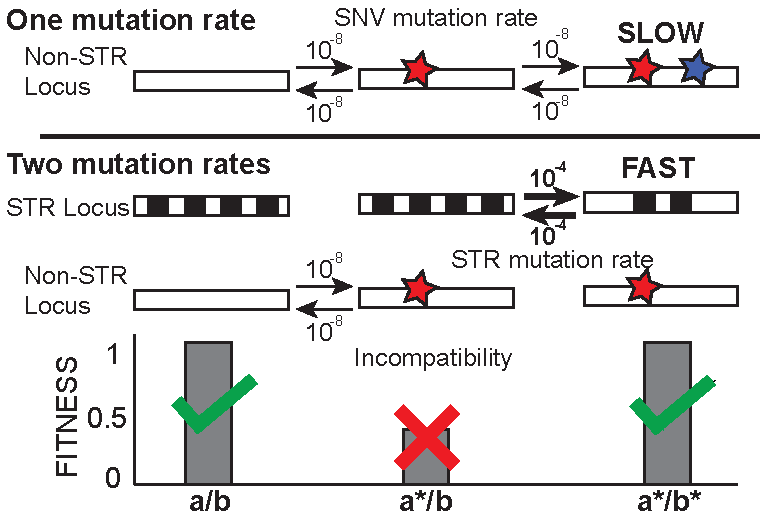
\includegraphics[width=6in]{tig_figs/repeatmumodel_051214.pdf}
\caption[A locus with higher mutation rates allows genetic modification of unfavorable genotypes at interacting loci.]{A locus with higher mutation rates allows genetic modification of unfavorable genotypes at interacting loci. Top, a model of evolution under epistasis with only one slow mutation rate. Middle, a model of evolution under epistasis with a slow and a fast mutation rate. Boxes represent loci, stars represent SNV-type mutations, black and white checkering indicates an STR locus (a/b, a*/b, and a*/b* signify different genotypes). Arrows with numbers represent possible mutations and their respective rates. Bottom, fitness of each genotype under both models. We expect that the model with two mutation rates will occupy the fully derived state (a*/b*) more quickly.
}
\label{fig:strfig2}
\end{figure}

\section{Modifier mutations leading to epistasis are expected in STRs.}
We have previously proposed that STRs might be more susceptible to genetic interactions \cite{Undurraga2012}, as we will briefly explicate here. Consider a simple two-locus haploid model under panmixis, in which loci A and B each start with a single allele ($ab$) and have the same probability $p$ per generation of mutating to a second allele ($a^*$ or $b^*$), with $p$ also as the probability per generation of reverting mutations (Figure ~\ref{fig:strfig2}). Let us further assume that A and B are in sign epistasis \cite{Weinreich2005} (that is, $a^*b$ and/or $ab^*$ have fitness less than $ab$ and $a^*b^*$). To escape the unfavorable $a^*b$ genotype, the organism may either revert to $ab$ or mutate forward to $a^*b^*$. When the A and B loci have equal mutation rates, we expect that the reversion of a single mutant is just as likely as a second mutation, and consequently that $a^*b^*$ individuals will appear only relatively rarely and slowly. However, consider a similar model, in which locus B has an elevated mutation rate $p_{b} > p_{a}$. In this case, the $a*b$ genotype has a higher probability of a second, modifying mutation to $a^*b^*$ than of a reversion to $ab$. Moreover, flux along the other mutational path ($ab \Rightarrow ab^* \Rightarrow a^*b^*$) will be increased. In sum, $a^*b^*$ genotypes will arise at higher rates, and will attain their equilibrium frequency much more rapidly, if either A or B has an elevated mutation rate \cite{Felsenstein2013} (p.131). This scenario can lead quickly to an equilibrium population in which incompatible epistatic alleles are frequent, even though recombinants have lower fitness. Relaxing the assumption of no population structure will further speed this process. Consequently, we would expect STRs and other loci with high mutation rates to be more likely to modify other alleles than loci with lower mutation rates, as long as we assume that all loci are equally capable of genetic interactions. This process may be referred to as 'coadaptation'. For a rigorous model of the evolution of hybrid incompatibility, see Orr \cite{Orr1995}.

\section{Analysis of selection on STR variation in \emph{A. thaliana}.}
If the predicted phenotypic effects of STR variation exist and are relevant, then we should be able to observe signatures of selection on STR variation. For SNV variation, measures such as $\omega$ (ratio of nonsynonymous to synonymous coding variants) and $\Pi$ (nucleotide diversity) can be used to assess this question, but for STRs no analogous measures exist. Consequently, we developed a heuristic method to estimate the ratio of observed to expected STR variation.

The unit number, unit length, and purity of a given STR locus in a high-quality reference genome predict its variation across individuals \cite{Legendre2007}. STRs with high unit number, short unit length, and high purity are typically highly variable. From population-scale STR genotype data \cite{Carlson2015}, we assessed the correlation of predicted variation of STRs (VARscore) and observed STR variation across A. thaliana strains.

\begin{figure}
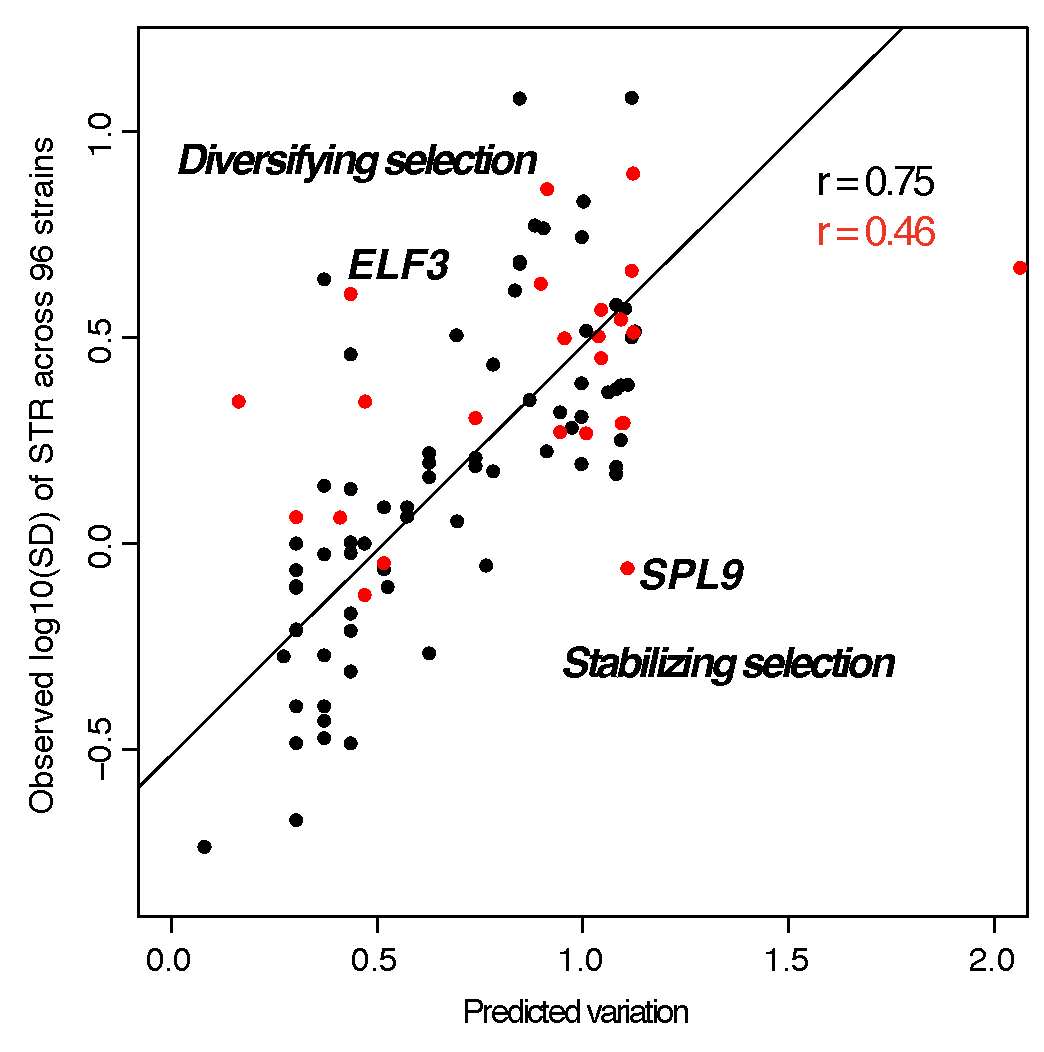
\includegraphics[width=4in]{tig_figs/logsd_varscore_011814.pdf}
\caption[Observed and predicted STR variation showed greater correlation for non-coding STRs than coding STRs. ]{Observed and predicted STR variation showed greater correlation for non-coding STRs than coding STRs. The correlation between the observed log10 of the standard deviation of STR unit number across strains (y-axis) and the VARscore (x-axis), which predicts STR variation from sequence characteristics. Black points are non-coding STRs, red points are coding STRs. Outliers may indicate functional importance (ELF3 STR is indicated).}
\label{fig:strfig3}
\end{figure}

In general, VARscore was well correlated with observed variation across STRs (r=0.68, Figure ~\ref{fig:strfig3}), a substantially better agreement than previously observed \cite{Duitama2014}. However, this correlation was substantially weaker among coding STRs (r=0.46) than among non-coding STRs (r=0.75). This discrepancy suggests that sequence characteristics alone do not suffice to predict whether coding STRs vary on a population scale. Coding STRs are more likely to be functionally important, and thus are less subject to the `neutral model' of the VARscore prediction. Deviation of predicted STR variation (i.e. VARscore) from observed variation may thus hold information about STR function and selective pressures acting upon it. Specifically, STRs that are observed to be more variable than predicted may be under diversifying selection, whereas those STRs that are observed to be less variable than predicted may be functionally constrained and under purifying selection. For example, the STR in the gene \emph{ELF3} is highly variable across strains, ranging from 7 units to as many as 29 units in a set of strains previously analyzed by Sanger sequencing \cite{Undurraga2012}. The phenotypes associated with variation in the \emph{ELF3}-STR change dramatically in different genetic backgrounds, suggesting co-evolution of the \emph{ELF3}-STR with epistatically interacting loci \cite{Undurraga2012}. Given this STR's strong background-dependent phenotypes, it is likely under diversifying selection and, correspondingly, it is much more variable than predicted. 

\section{Concluding remarks}
The study of STRs and other under-ascertained genomic elements has the potential to reshape our model of the heritability of complex diseases and traits, both in terms of the overall proportion of heritability explained, and in terms of the components of heritability themselves . Experimental studies in model organisms have taught us that the phenotypic effects of genome-wide STR variation are both dramatic and impossible to understand without taking epistasis into account. In the future, our understanding will be improved by 1) accurate STR population-scale genotyping, 2) more appropriate statistical methods for analyzing STR-phenotype associations, and 3) a broader description of epistasis between STR variation and other loci in determining phenotype.

% ========== MAX put in a chapter here
\chapter{The variable ELF3 polyglutamine hubs an epistatic network}

\footnotetext{
Supporting figures and tables can be found in Appendix D.
}

\section{Abstract}
Short tandem repeats are hypervariable genetic elements occurring frequently in coding regions. Their fast mutation rate has been recognized as a potent source of genetic variation contributing to adaptive evolution and the heritability of human disease. We recently proposed that such repeats are likely to mediate epistasis, by supplying compensatory mutations in certain genetic backgrounds. We have previously described one such case, in the \emph{A. thaliana} gene \emph{ELF3}, of a short tandem repeat that encodes a highly variable polyglutamine. In a twofold approach, we 1) dissected the genetic architecture of this incompatibility between two \emph{A. thaliana} ecotypes, and 2) used a yeast two-hybrid strategy to identify proteins whose physical interactions with ELF3 were modulated by polyglutamine status. Using these two orthogonal approaches, we identify specific genetic and physical mechanisms by which the \emph{ELF3} repeat may mediate the observed genetic incompatibilities. Our work elucidates a variety of mechanisms by which repeat variation, which is generally underascertained in population-scale sequencing, can control phenotypic variation. Furthermore, our work suggests that such highly variable loci contribute disproportionately to the epistatic component of heritability. 

\section{Introduction}
It is often commented that evolution is not a designer but a tinkerer \cite{Jacob1977,Alon2003}. That is, adaptations are generally short-term, incremental fixes rather than alterations in fundamental biological plans. This principle is believed to underlie many design properties of biological systems. One source of genetic variation for such tinkering lies in short tandem repeats (STRs), genetic elements with elevated mutation rates. From these mutation rates, it is believed that STRs are thus more likely than substitutional variants to contribute adaptive variants on a per-locus basis \cite{Kashi1997,Gemayel2010,Hannan2010}. It is also plausible that many (or most) adaptations are in fact compensations for other genetic variants \cite{Szamecz2014}. Consequently, it is expected that STRs are relatively likely to show epistasis with other loci, and this expectation is borne out in the handful of well-characterized STRs \cite{Press2014}. 

One such STR resides in the Arabidopsis thaliana gene \emph{ELF3}, where it encodes a polyglutamine that varies dramatically in length across different natural isolates \cite{Tajima2007,Undurraga2012}. We have previously shown that these \emph{ELF3}-STR variants have strong effects on phenotype, but these effects differ depending on the genetic background hosting the variant in question \cite{Undurraga2012}. These observations suggest variants in the background modifying the effect of STR alleles through epistasis. The high variability of the \emph{ELF3}-STR relative to expectations suggests that this STR may be compensating for variation in several genes across strains of \emph{A. thaliana} \cite{Carlson2015}, according to epistatic variants specific to each strain. Previously, ELF3 was found to serve as a QTL affecting levels of ``stochastic noise'' in the phenotypes of recombinant inbred lines of A. thaliana \cite{Jimenez-Gomez2011,Lachowiec2015}. These observations invite comparison to known ``robustness genes'' such as Hsp90 \cite{Sangster2007,Sangster2008,Sangster2008a}, which act by revealing or concealing genetic variants affecting phenotypes. One potential mechanism of this robustness phenomenon is that such genes are highly connected in genetic networks. These previous observations lead to an expectation that ELF3 lies at the center of epistatic networks determining phenotypic variation in \emph{A. thaliana} phenotypes. However, it is not clear to what degree variation in the ELF3 polyQ may contribute to this phenotypic variation. 

The ELF3 protein functions promiscuously as an adaptor protein in multiple protein complexes involved in a variety of developmental pathways \cite{Liu2001,Yu2008,Yoshida2009,Nusinow2011,Chow2012}. Consequently, a favorable hypothesis for why \emph{ELF3-STR} variation affects phenotypes is that the encoded polyglutamine affects ELF3's interactions with these other proteins. The ELF3 C-terminus, which contains the STR-encoded polyglutamine, is necessary for nuclear localization \cite{Herrero2012} and ELF3 homodimerization \cite{Liu2001}, but only one other protein (Phytochrome Interacting Factor 4, PIF4) has been shown to interact with this domain of ELF3 \cite{Nieto2014}. These observations suggest naively that any effect of the ELF3-polyQ is likely to be derived from ELF3 protein-protein interactions mediating ELF3 nuclear localization or regulation of the PIF4 developmental integrator. 

As an alternative hypothesis for how the \emph{ELF3-STR} affects phenotype, one study of an intronic STR in \emph{A. thaliana} demonstrated that certain hyperexpanded STR alleles led to dysregulation of the \emph{IIL1} gene \cite{Sureshkumar2009}, presumably due to the difficulty of processing this expanded STR in \emph{IIL1} transcripts. It is possible that, rather than modulating normal ELF3 function as an encoded polyglutamine, the \emph{ELF3-STR} affects \emph{ELF3} transcript or protein function. It has been previously argued that such 'informational' (as opposed to 'operational') genomic processes are more likely to have genetic or physical interactions \cite{Jain1999}. Therefore, it is not clear whether we should expect that the incompatibilities arise from altered ELF3-protein interactions, or whether they are the effect of altered processing of ELF3 transcripts or proteins in different backgrounds.

In this study we dissect the epistatic landscape modifying the function of the \emph{ELF3-STR} through both physical and genetic interactions, and present evidence that this STR forms the hub of a complex network of epistasis, likely due to its role as a compensatory modifier of many other loci. Furthermore, we present data suggesting that the altered protein-binding function of ELF3 is unlikely to fully explain the polyQ-mediated background effect. 

\section{Materials and Methods}
\subsection{Plant material and growth conditions}
Hypocotyl length was assayed in seedlings grown for 15d in incubators set to SD 22$\degree$ on vertical plates as described previously \cite{Undurraga2012}. The \emph{elf3-200} \cite{Undurraga2012} and \emph{elf3-4} \cite{Hicks1996} mutants have been previously described. T-DNA lines \cite{Alonso2003,Kleinboelting2012} were obtained from the Arabidopsis Biological Resource Center (Ohio State University), and are given in Table ~\ref{tab:app5tab2}. 

\subsection{Genotyping}
For genotyping the ELF3 STR and other loci across many $F_{2}$ segregants, 1-2 true leaves from each seedling were subjected to DNA extraction as previously described \cite{Undurraga2012}. Seedlings were stored on their growth plates at 4$\degree$ before genotyping but after phenotypic analysis. For the ELF3 STR, PCR was performed in 10 $\mu$L volume containing 0.5 $\mu$M primers (Table ~\ref{tab:app5tab1}), 0.2 $\mu$M each dNTP, 1 $\mu$L 10X ExTaq buffer, and 0.1 U ExTaq (Takara, Tokyo, Japan); with initial denaturation step of 95$\degree$ for 5', followed by 40 cycles of 95$\degree$ 30'', 49$\degree$ 20'', 72$\degree$ 10'', with a final extension step at 72$\degree$ for 5'. For other loci, PCR was performed in 20 $\mu$L volume containing 0.5 $\mu$M primers (Table ~\ref{tab:app5tab1}), 0.2 $\mu$M each dNTP, 2 �L 10X ExTaq buffer, and 0.25 U Taq polymerase (NEB, Ipswich, MA); with initial denaturation step of 95$\degree$ for 5', followed by 35 cycles of 95$\degree$ 30'', 55$\degree$ 30'', 72$\degree$ 1', with a final extension step at 72$\degree$ for 5'.

\subsection{Genome resequencing}
Plants selected for genotyping-by-sequencing were transplanted to soil and grown under LD for 2-3 weeks. They were then stored at 4$\degree$ until DNA extraction was performed. One late rosette-stage Ws individual was used for Ws whole-genome resequencing. DNA extraction was performed using the DNeasy Plant Mini kit (Qiagen, Valencia, CA) according to the kit protocol. This DNA was quantified using high-sensitivity Qubit fluorescence analysis (ThermoFisher Scientific, Waltham, MA) and re-genotyped with \emph{ELF3-STR} primers (Table ~\ref{tab:app5tab1}). We used 10 ng DNA from each $F_{2}$ segregant in NextEra transposase library preparations (Illumina, San Diego, CA), or a standard 50 ng preparation for the Ws library. Library quality was assessed on a BioAnalyzer (Agilent, Santa Clara, CA) or agarose gels. The Ws individual was sequenced in one 300-cycle MiSeq v2 run (300 bp single-end reads) to ~12X coverage. Ws sequence data will be deposited with the 1001 Genomes Project. The F2 segregant libraries were pooled and sequenced in one 200-cycle HiSeq v3 run to ~2X average coverage (100 bp paired-end reads, Table ~\ref{tab:app5tab3}). $F_{2}$ genotype data in VCF and QTL format are available on request.

\subsection{Sequence analysis}
Reads were aligned to the Col reference genome using BWA v0.7.5 MEM \cite{Li2013}, and variants were called using SAMtools v0.1.19 \cite{Li2009}. High-quality Ws variants (Q>=40) were thus identified from Ws parent data, and compared with variants in previously-sequenced related strains \cite{Gan2011}. $F_{2}$ segregant genotype calls were combined into a single variant call format (VCF) file and filtered for loci with such Ws variants. We used SNPtools (WANG et al. 2013) to perform haplotype and genotype imputation for each locus in $F_{2}$ segregants. For workflows employed in sequence analysis, see Appendix D. Genotype data are available on request. Following sequence analysis, one individual was found to be a heterozygote at the \emph{ELF3} locus. This individual was omitted from all following analyses requiring \emph{ELF3} homozygotes.

\subsection{Quantitative trait locus (QTL) analysis}
$F_{2}$ genotypes were reduced to a set of 500 loci randomly sampled from the imputed genotypes, plus a single nucleotide variant (SNV) marking the \emph{ELF3} locus. We used these genotypes to estimate a genetic map and perform QTL analysis using the R/qtl package \cite{Broman2003}. A nonparametric epistasis test was implemented in a custom R script using R/qtl functions. For a more detailed description of commands and the epistasis test, see  Appendix D. Follow-up genotyping of additional $F_{2}$s was performed using PCR markers (Table ~\ref{tab:app4tab1}), and these genotypes were included in subsequent QTL analyses. 

\subsection{Candidate gene analysis}
Homozygous T-DNA lines \cite{Alonso2003,Kleinboelting2012} with insertions in genes of interest were obtained from the Arabidopsis Biological Resource Center (Ohio State University) and phenotyped for hypocotyl length under SD at 15 days. All such experiments were repeated at least once. Double mutants were obtained by crossing relevant lines and genotyping (primers in ~\ref{tab:app4tab1}). Mutant lines are listed in Table ~\ref{tab:app5tab2}.
 
\subsection{Yeast two-hybrid}
 ELF3 variants with different STR lengths were PCR cloned out of cDNAs of previously described A. thaliana carrying \emph{ELF3} transgenes \cite{Undurraga2012} into the XmaI/BamHI sites of pGBKT7. Genes to be tested for ELF3 interactions were PCR cloned into the EcoRI/XhoI sites of pGADT7 from cDNAs of indicated strains (Table ~\ref{tab:app4tab1} for primers). Clones were confirmed by restriction digest and sequencing. The Y2H screen was performed against the Arabidopsis Mate and Plate cDNA library (Clontech, Madison, WI), essentially according to the manufacturer's instructions, except selections were performed on C-leu -trp -his plates incubated at 23$\degree$. Clones which also showed activation of the \emph{ADE2} reporter gene and did not autoactivate were subsequently tested against the various ELF3-polyQ constructs (see Appendix D for details, full details on clones available upon request).

LacZ activity was assayed through X-gal cleavage essentially as previously described, again in strains using PJ69-4$\alpha$ as Mat$\alpha$ parent \cite{Mockli2004}. For weakly activating constructs (GLDP1 and ELF4), 0.2 absorbance units of yeast were used in each assay to reduce background, and color development was assessed at points between 16 and 72 hours of incubation at room temperature. 

Quantitative PCR (qPCR): For measuring ELF3 and LSH9 transcript levels, pooled aerial tissue of ~30 mg short-day-grown seedlings of each relevant genotype were collected at ZT8 7d post germination. RNA preparation and qPCR was performed as described previously \cite{Undurraga2012}, using primers in Table ~\ref{tab:app5tab1}.

Statistical analysis: All statistical analyses and plotting was performed using R 2.15.3 or R 3.2.1 \cite{RCoreTeam2016}. Analysis scripts are available upon request.

\section{Results}
To investigate the genetic architecture of epistasis for the \emph{ELF3-STR}, we crossed two \emph{A. thaliana} strains with a previously reported mutual incompatibility of their respective \emph{ELF3-STR} variants (Col-0, Ws, \cite{Undurraga2012}). We generated an $F_{2}$ population from this cross, which we phenotyped for variation in hypocotyl length under short days (SD), a trait dramatically affected by ELF3 function. The Col and Ws backgrounds do not substantially differ in this trait (p = 0.16, Kolmogorov-Smirnov test, Figure ~\ref{fig:chap5fig1}A). We found that most $F_{2}$s showed phenotypes within the range of the two parental lines, except that the $F_{2}$ phenotypic distribution had a long upper tail of transgressive variation, and consequently a different distribution from either parent (p = 0.0039 against Ws, p = 0.055 against Col, Kolmogorov-Smirnov tests). Longer hypocotyls in light conditions indicate ELF3 dysfunction in the circadian clock \cite{Liu2001,Hicks2001}, consistent with the co-segregation of incompatible Col and Ws alleles. These observations indicated that the previously observed ELF3 background effect \cite{Undurraga2012} was present in this segregating population. We next replicated this observation in a much larger population (1106 seedlings), which was used for further genetic analysis. 
 
\begin{figure}
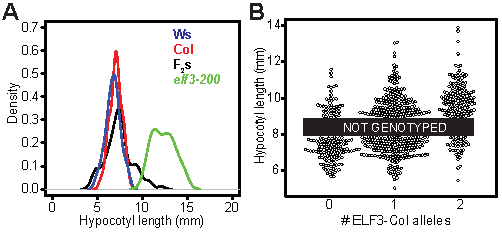
\includegraphics[width=6in]{elf3_epi/elf3_fig1_121615.pdf}
\caption[Phenotypic transgression for 15d hypocotyl length under short days in Col x Ws $F_{2}$ segregants.]{Phenotypic transgression for 15d hypocotyl length under short days in Col x Ws $F_{2}$ segregants. (A): $F_{2}$ segregant phenotypes compared to parents and an elf3 mutant; n $\approx$ 50 for each homozygous line and n $\approx$ 100 for $F_{2}$s. Colors indicate genotypes. (B): Phenotypic distributions of a large population of Col x Ws $F_{2}$ segregants, for 720 extreme individuals genotyped at the ELF3 locus. N = 1106 seedlings. 386 ungenotyped individuals fall into the region indicated by the black box.}
\label{fig:chap5fig1}
\end{figure}
 
\subsection{Genetic analysis of ELF3-STR effects on hypocotyl length}
We investigated the genetic basis of the phenotypic transgression in hypocotyl length by harvesting the 720 most phenotypically extreme seedlings (longest and shortest hypocotyls) for genotyping (Figure ~\ref{fig:app5fig1}). We genotyped each such individual at the \emph{ELF3} locus, using primers directly ascertaining the 27bp \emph{ELF3-STR} polymorphism between Col and Ws. Across these individuals, we observed a strong main effect of the ELF3 locus on the phenotype (Figure ~\ref{fig:chap5fig1}B), in which the Col allele of ELF3 is substantially more likely to show transgressive phenotypes implying incompatibility, though individuals homozygous for the Ws allele also show transgressive phenotypes. 

Among these seedlings, much of the information about genetic effects of ELF3 on hypocotyl length was contained in the individuals with extreme phenotypes, and individuals homozygous at the \emph{ELF3} locus. ELF3 genetic interactions are expected to be most apparent in \emph{ELF3} homozygotes. Consequently, we used a novel genetic approach to detect epistasis between ELF3 and other loci as follows. For each \emph{ELF3-STR} allele, we selected the 24 homozygotes of each sort (Ws/Ws and Col/Col) at each phenotypic extreme (the shortest and longest hypocotyls). The sampling of extremes is an effective and statistically justified method for genetic mapping (LANDER and BOTSTEIN 1989). These 96 individuals were analyzed in a genotyping-by-sequencing approach (Table ~\ref{tab:app5tab3}, Figure ~\ref{fig:app5fig1}). 

We also resequenced the genome of the Ws (Wassilewskija) parent to ~12X coverage, calling $3.2*10^5$ variants relative to Col, and used these variants as identifiers for Ws haplotype blocks. Comparisons of single nucleotide variants (SNVs) with related \emph{A. thaliana} strains Ws-2 and Ws-0 yielded substantial overlap but also significant variation (Figure ~\ref{fig:app5fig2}), indicating good SNV ascertainment. For each F2 individual, we mapped reads to the Col-0 reference and imputed haplotypes across each of the 96 individuals to identify chromosome blocks inherited from each parent Figure ~\ref{fig:app5fig3}. 

With this data, we performed a one-dimensional QTL scan to identify chromosomal regions contributing main effects to hypocotyl length (Figure ~\ref{fig:chap5fig2}A). This analysis indicated a peak on Chr2 corresponding to \emph{ELF3} as expected, but also larger peaks on Chr1, Chr4, Chr5, and potentially one or more additional peaks on Chr2 affecting the phenotype. Ten additional $F_2$s were genotyped by PCR around these peaks. A two-dimensional QTL scan suggested that at least some of these peaks interact epistatically with the ELF3 locus (Figure ~\ref{fig:app5fig4}). 

We binned $F_{2}$s homozygous at ELF3 according to their ELF3 genotype, and performed one-dimensional QTL analysis on each homozygote group separately (masking the genotypes of all other individuals). We observed that the same LOD peaks were replicated well in ELF3-Col homozygotes, but poorly in ELF3-Ws homozygotes (Figure ~\ref{fig:chap5fig2}B). Notably, Chr2 signal remained, indicating that the other loci on Chr2 are relevant to the phenotype (at least in ELF3-Col plants). This analysis suggested that the ELF3-STR genotype is epistatic to the other loci controlling this phenotype, with effects masked in ELF3-Ws plants. 

\begin{figure}
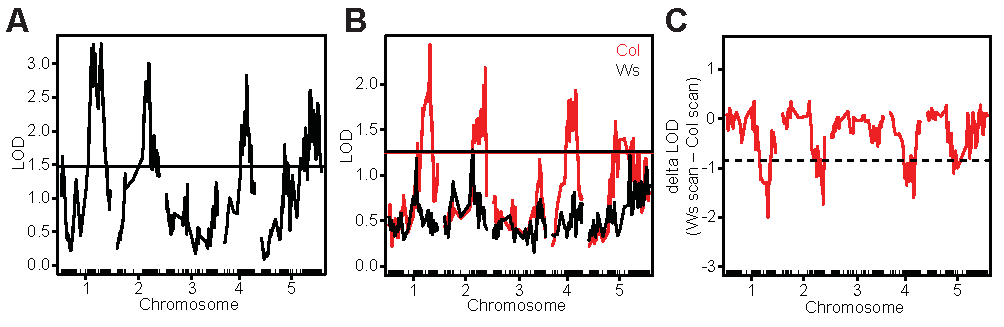
\includegraphics[width=6in]{elf3_epi/elf3_fig2_qtl_121615.pdf}
\caption[QTL analysis identifies interactions of ELF3 with multiple loci.]{QTL analysis identifies interactions of \emph{ELF3} with multiple loci. (A): one-dimensional QTL scan including all $F_{2}$s. Horizontal line indicates 99\% significance threshold based on permutations. (B): QTL scan stratified by \emph{ELF3} genotype (all genotypes but those of indicated $F_{2}$s masked in each analysis). Horizontal lines of each color indicate 99\% significance threshold based on permutations for each scan.  (C): A direct nonparametric test of epistasis between \emph{ELF3} and other loci, using the independent QTL scans shown in (B). \emph{ELF3} is located on chromosome 2. Dotted horizontal line indicates 99\% significance threshold based on simulations.}
\label{fig:chap5fig2}
\end{figure} 

To directly test for epistasis with \emph{ELF3}, we adapted a previously described method \cite{Sangster2008a}. Separating the ELF3 homozygotes again, we used permutations to define an empirical null distribution for the difference of likelihood (LOD) scores expected between the Ws and the Col scans. When comparing the difference in LOD scores between the two QTL scans at all loci, we found that the peaks on Chr1, Chr2, and Chr4 (and to a lesser extent Chr5) were all stronger in Col (Figure ~\ref{fig:chap5fig2}C). Consequently, these loci constitute background-specific ELF3 interactors.  

We considered the genetic contribution of these loci to the phenotype using a multiple QTL mapping approach, using both the independently estimated QTL locations and a refined model re-estimating QTL positions based on information from all QTLs (Table ~\ref{tab:app5tab4}). In each case, strong effects on Chr1, Chr2, and Chr4 were supported, along with interactions between Chr2 (\emph{ELF3}) and the other two loci. In the refined model, the Chr5 locus and a second Chr2 locus are also strongly supported. We conclude that while \emph{ELF3} interacts epistatically with a variety of other loci in determining hypocotyl elongation, the principal contributors to ELF3-mediated effects on the trait are on Chr1 and Chr4. Inspection of the phenotypes of genotype combinations between ELF3 and each locus supported the hypothesis of epistasis with \emph{ELF3} for most QTLs (Figure ~\ref{fig:app5fig5}). 

\subsection{Candidate gene analysis}
The chromosome intervals identified by our QTL analysis were fairly large, as we were limited in resolution by the recombination events occurring in the sequenced segregants. These large intervals include a large number of potential candidate genes, and overlapped with a 1.8 MB inversion between these backgrounds on Chr4 \cite{Rowan2015}. Previous analyses mapping variation in hypocotyl length have detected loci in these regions and screened candidate genes for hypocotyl phenotypes \cite{Khattak2014}. 
	
We attempted to both replicate several such observations and investigate novel loci in the Col background under the conditions of our intercross experiment (15d SD hypocotyl length). We were able to confirm small phenotypic effects of T-DNA insertion mutants \emph{lsh9} and \emph{nup98} (Figure ~\ref{fig:app5fig6}), but it is unlikely that these additive effects on their own explain the phenotypic variation in $F_{2}$s (Figure ~\ref{fig:chap5fig1}A). 

\begin{figure}
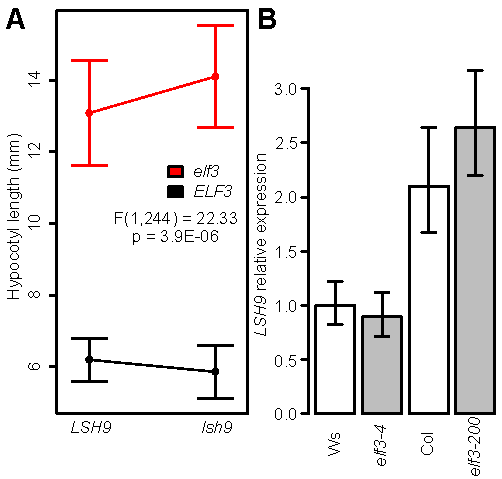
\includegraphics[width=3in]{elf3_epi/lsh9_elf3_fig3_030316.pdf}
\caption[\emph{ELF3} shows a genetic interaction with \emph{LSH9} and modulates its expression in a background-specific fashion.]{\emph{ELF3} shows a genetic interaction with \emph{LSH9} and modulates its expression in a background-specific fashion. (A): Double mutant analysis of \emph{elf3} and \emph{lsh9} seedlings grown 15d under SD. Statistics shown are from ANOVA analysis of the interaction between the mutant effects on phenotype. Error bars indicate standard deviation, n > 35 for each genotype. (B): Reverse-transcriptase PCR (RT-PCR) analysis of \emph{LSH9} expression across genotypes. Seedlings were grown short days and harvested for RNA at ZT8 (dusk). \emph{LSH9} expression is expressed as a proportion of Ws expression, normalized relative to \emph{UBC21}, error bars are standard error from three technical replicates. Experiments were repeated with similar results.}
\label{fig:chap5fig3}
\end{figure} 

We generated double mutants between mutants affecting hypocotyl length and \emph{elf3}, to establish whether these genes operated in the same pathway as ELF3. We found evidence for an interaction between \emph{ELF3} and \emph{LSH9}, in the form of reciprocal sign epistasis between the two null mutants affecting SD hypocotyl length (Figure ~\ref{fig:chap5fig3}A). While \emph{lsh9} single mutants had slightly shorter hypocotyls than WT, \emph{lsh9 elf3} double mutant hypocotyls were longer than in \emph{elf3} single mutants. We found no evidence for an interaction between nup98 and elf3 mutations (Figure ~\ref{fig:app5fig6}C). LSH9 (LIGHT SENSITIVE HYPOCOTYLS 9) is an uncharacterized protein from a family of paralogs named for LSH1, which acts in light regulation of hypocotyl elongation \cite{Zhao2004}. Like other members of its family, it contains a putative nuclear localization sequence but few other distinguishing features. We were unable to detect a physical interaction between the Col or Ws variants of LSH9 and ELF3 using yeast two-hybrid (Y2H, Figure S7), suggesting that \emph{ELF3-LSH9} epistasis is not based upon a physical interaction between the two proteins. Levels of \emph{LSH9} transcript were no different between WT and \emph{elf3} mutants in either the Col or the Ws backgrounds relative to WT, but were reduced overall in the Ws background relative to Col (Figure ~\ref{fig:chap5fig3}B). Furthermore, \emph{ELF3} expression levels were unchanged in \emph{lsh9} mutants relative to Col (Figure ~\ref{fig:app5fig8}). Consequently, \emph{ELF3-LSH9} epistasis between Col and Ws may be due to regulatory changes between these two backgrounds altering \emph{LSH9} transcript levels. This interpretation is consistent with the much stronger effect of this QTL in an \emph{ELF3-Col/ELF3-Col} background (Figure ~\ref{fig:app5fig5}). However, this epistasis is unlikely to be due to a direct physical or regulatory interaction. 

\begin{figure}
\includegraphics[width=5in]{elf3_epi/figure_y2helf4phyb_fig4_030316-01.png}
\caption[Y2H interaction of ELF3 with known protein interactors can be modulated by polyQ variation. ]{Y2H interaction of ELF3 with known protein interactors can be modulated by polyQ variation. Yeast carrying indicated vectors were spotted in five-fold dilutions onto C-leu-trp (C-LT) or C-leu-trp-his-ade (C-LTHA) media. PHYB-Cterm: previously-defined C-terminal truncations of PHYB sufficient for ELF3 interaction \cite{Liu2001} from the Col and Ws backgrounds. For each protein X, experiments were repeated with independent PJ69-4$\alpha$ + pGADT7-X transformants with similar results.}
\label{fig:chap5fig4}
\end{figure} 

\subsection{ELF3-polyQ variation's effect on known protein interactions}
In parallel with our genetic analysis, we also used Y2H analysis to directly identify proteins whose physical interactions with ELF3 are polyQ-modulated. We first attempted to confirm that synthetic ELF3s with 0Q (no polyQ), 7Q (variant in Col), 16Q (variant in Ws), and 23Q (endogenous to strains Br-0 and Bur-0) forms of ELF3 show Y2H interactions with well-described ELF3 interactors ELF4 \cite{Nusinow2011,Herrero2012} and PHYB \cite{Liu2001} (Figure ~\ref{fig:chap5fig4}). None of the ELF3 constructs showed auto-activation in yeast also carrying an empty vector (Figure ~\ref{fig:app5fig9}). The ELF3-interacting domain of PHYB has two coding variants between Col and Ws, and we thus tested both Ws and Col variants of this domain, and found that both forms showed apparently equal affinity with all polyQ variants of ELF3 (Figure ~\ref{fig:app5fig9}A). ELF4, which has no coding variants between Col and Ws, interacted with all polyglutamine variants of ELF3 (Figure ~\ref{fig:app5fig9}B), though rather weakly compared to PHYB. Under these conditions, a subtle apparent preference of ELF4 for longer polyQ variants (e.g. ELF3-16Q and ELF3-23Q) was repeatable. 
	
Recently, it was reported that ELF3 interacts with the transcription factor PIF4 both in Y2H and \emph{in planta} \cite{Nieto2014}. We were not able to replicate this finding for any ELF3-polyQ variant in our Y2H system (Figure ~\ref{fig:app5fig10}A, or using an alternate strain background, Y187, Figure ~\ref{fig:app5fig10}B), and were thus unable to evaluate effects of polyQ variation on ELF3-PIF4 interactions. Future work with alternate methods may reveal such effects. 
	
Collectively, these data suggest that the ELF3-polyQ's effect on ELF3 protein-protein interactions is more efficacious for marginal interactions, which are presumably more sensitive to structural variation in ELF3. However, to demonstrate that specific interaction differences play a role in previously described phenotypic effects of ELF3-polyQ variation, more work will be necessary.

\begin{figure}
\includegraphics[width=6in]{elf3_epi/elf3_fig5_y2hscreen-01.pdf}
\caption[Y2H screen identifies new interactors of ELF3.]{Y2H screen identifies new interactors of ELF3. (A): ELF3 Y2H screen design. (B): Yeast carrying indicated vectors were spotted in five-fold dilutions onto C-leu-trp (C-LT) or C-leu-trp-his-ade (C-LTHA) media. For each protein X, experiments were repeated with at least two independent PJ69-4$\alpha$ + pGADT7-X transformants with similar results.}
\label{fig:chap5fig5}
\end{figure} 

\subsection{Y2H screen for new interactors}
None of these known ELF3 interactors were encoded by genes located in the major (Chr1, Chr4) QTLs identified by our genetic screen. If the ELF3-polyQ mediates protein interactions, we would expect that these regions contain additional, previously-undescribed ELF3 interactors which vary between the Col and Ws backgrounds. We screened the ELF3-7Q for interactions with proteins from a commercially available library derived from Col, to detect ELF3-protein interactions within the Col background. 
	
We subjected positives in the Y2H screen to several rounds of confirmation (Appendix F), leaving a total of 3 robust, novel proteins interacting with ELF3: LUL4, AtGLDP1, and PLAC8-domain-containing protein AT4G23470 (Figure ~\ref{fig:chap5fig5}). AT4G23470 was recovered in two independent clones, and LUL4 was recovered in three independent clones. The PLAC8-domain protein is encoded by a gene within the QTL interval on chromosome 4, but this protein showed no evident preference for any polyQ variant of ELF3, and thus differential interaction with this protein is unlikely to underlie the observed epistasis. One protein, AtGLDP1, appeared to show a subtle preference for the ELF3-0Q construct over longer polyQs. While this screen is unlikely to exhaust hitherto-unknown ELF3 interactors, and all interactions require confirmation \emph{in planta}, these data support a model in which the ELF3-polyQ does not dramatically affect ELF3's interactions with other proteins. Other mechanisms for genetic interactions with any given loci are not informed by this Y2H analysis. 

\subsection{Subtle variation in ELF3 affinity for other proteins mediated by polyQ variation}
Two proteins, ELF4 and GLDP1, showed slight variation among polyQ variants of ELF3 in the Y2H growth assay. Both proteins showed relatively weak interactions with ELF3, and thus it was difficult to quantify the effect of the ELF3-polyQ on these interactions by yeast cell growth under selection. We therefore assayed LacZ expression by the Y2H constructs directly and quantitatively by measuring X-gal cleavage (Figure ~\ref{fig:app5fig11}). This assay supported subtle effects of the polyQ, with GLDP1 slightly preferring shorter polyQs (particularly the synthetic ELF3-0Q), and ELF4 slightly preferring longer polyQs (particularly ELF3-16Q). These results suggest that polyQ effects on interactions with other proteins, though small, may be important for metastable ELF3-protein interactions, although strong protein interactions (for example ELF3-LUL4, ELF3-PHYB) are apparently robust to polyQ variation. 

\section{Discussion}
The contribution of STR variation to complex traits has been speculated for some time to be considerable \cite{Kashi1997,Press2014}. Specifically, it is expected that STR variation may contribute disproportionately to the epistatic term of genetic variance, and the molecular mechanisms by which different STRs contribute are expected derive from their specific features. For instance, polyQ variation may be expected to affect the protein interactions \cite{Schaefer2012,Stott1995} and the transactivation activity of affected proteins \cite{Escher2000}. In this study, we considered these questions in the case of the previously-described \emph{ELF3-STR} \cite{Undurraga2012}. We found that the genetic architecture of ELF3-dependent phenotypes is highly epistatic between the Col and Ws strains, leading to substantial phenotypic transgression in the phenotype of hypocotyl length. We identified several candidates for loci underlying the observed ELF3 interaction, and confirmed that one gene (\emph{LSH9}) showed a genetic interaction with \emph{ELF3}. Next, we used Y2H screening of ELF3-protein interactions to investigate whether the molecular mechanism of ELF3 STR effects could be disrupted protein interactions. We found evidence that variation in the STR-encoded ELF3 polyQ was sufficient to subtly modulate weaker ELF3-protein interactions, notably with the proteins ELF4 and AtGLDP1. These findings support a model in which highly variable loci, in particular STRs, can contribute to the epistatic component of heritability through both direct and indirect functional interactions with other loci.

\subsection{Potential genetic interactors of \emph{ELF3}}
We identified at least 3 QTLs showing genetic interactions with the \emph{ELF3-STR} in a Col x Ws cross. These QTLs generally did not coincide with obvious candidates. Previous work has, however, found QTLs in similar regions for hypocotyl traits \cite{Khattak2014}. The confirmation of one genetic interaction (\emph{LSH9}) in the Col background suggests that these QTLs underlie variants truly affecting hypocotyl length in tandem with \emph{ELF3-STR} variation. Further work will be necessary to more precisely map these variants. 
	
\subsection{The ELF3-polyQ and physical protein interactions}
We applied an orthogonal method, Y2H, to study potential effects of polyQ variation on ELF3's interactions with other proteins. ELF3's promiscuous physical associations with other proteins are known to be essential to its functions in the circadian clock \cite{Nusinow2011,Herrero2012} and flowering repression \cite{Liu2001,Yu2008}. Disruption of these interactions suggested an attractive mechanism by which ELF3 polyQ variation might affect ELF3 function. Assaying several known and novel ELF3-interacting proteins yielded evidence for a small effect of polyQ variation on metastable protein interactions, but no generic requirement for ELF3 polyQ status across proteins. Indeed, the modest effects that we found were protein-specific and thus not likely to generalize. We have, of course, not exhausted all possibilities for polyQ-dependent protein interactions, and our data must be considered provisional pending \emph{in planta} analysis of interactions. 
	
We do find that the ELF3-ELF4 interaction, which is crucial for circadian function and thus hypocotyl length \cite{Nusinow2011,Herrero2012}, demonstrates a subtle preference for the Ws 16Q ELF3 variant. The lack of sequence variation in ELF4 between Col and Ws and our failure to map the \emph{ELF4} locus by QTL analysis suggest that this difference alone does not underlie the transgressive phenotypes revealed by \emph{ELF3-STR} variation (Figure ~\ref{fig:chap5fig1}A). However, the slight polyQ-dependence of the ELF3-ELF4 interaction could be important in higher-order interactions. 
	
An alternative hypothesis is that ELF3-polyQ length is related to activation of regulatory targets of the EC. One point in favor of this hypothesis as the mechanism of ELF3-polyQ function is that relatively few of ELF3's interactors have been shown to require the polyQ-residing C-terminus of ELF3. We do not address this hypothesis, though future experiments measuring EC occupancy at target promoters or target transcription under different polyQ regimes could provide some answers.

\subsection{ELF3 as a robustness gene}
An alternate hypothesis to direct, identifiable strong genetic interactions of ELF3 explaining polyQ-dependent genetic architectures is that there are many weak interactions that can be perturbed by hypomorphic ELF3 activity. In this interpretation, ELF3 is a ``robustness gene'' \cite{Lempe2013}. The best-described example of such is in the protein chaperone HSP90 \cite{Rutherford1998}, whose multiple interactions with proteins in a variety of signaling pathways \cite{Taipale2012} lead to pleiotropic effects upon HSP90 inhibition or dysregulation \cite{Sangster2007}. ELF3 has been previously proposed as a robustness gene \cite{Jimenez-Gomez2011}, based on its promiscuity in protein complexes and the pleiotropic nature of \emph{elf3} phenotypes. Our finding that functional modulation by polyQ variation reveals several genetic interactors supports this interpretation, though it is unclear whether the effects are strong enough to bear the comparison. 
	
A similar hypothesis is that ELF3 ``gates'' robustness effects from robustness genes with which it interacts. For instance, we have recently shown that ELF3 function is epistatic to some of HSP90's pleiotropic phenotypic effects (M. Zisong, M. Press, P. Rival, C. Queitsch, and S.J. Davis, unpublished data) and \emph{ELF4} has also been proposed as a robustness gene governing circadian rhythsms and flowering \cite{Lempe2013}. We suggest in this paper that polyQ variation affects ELF3-ELF4 binding, which would provide a mechanistic link between ELF3 polyQ effects and a known robustness gene. 

These hypotheses remain speculative in the absence of more explicit tests. Nonetheless, we suggest that the pleiotropic effects of polyQ variation in ELF3 may be better understood by using robustness variation as a model. 

\subsection{General implications for polyQ variation}
PolyQ variation is best-known for the role of certain polyQ hyperexpansions in human neurological disorders \cite{Orr2012}. For instance, the degree of huntingtin polyQ expansion is strongly correlated with Huntington's disease severity \cite{Andrew1993}. However, there are a variety of differences between the ELF3 polyQ and these cases. These hyperexpansions are often associated with protein aggregation or plaque formation, a phenomenon that requires a sufficiently long uninterrupted polyglutamine domain \cite{Stott1995,Sharma1999,Lu2015}. These previous \emph{in vitro} studies suggest that although the ELF3 polyQ variants in Col and Ws are sufficiently different to alter phenotype, neither is long enough to lead to aggregation by these mechanisms (though the 23Q variant may be within this range). Furthermore, no ELF3-polyQ-related phenotype has been shown to have a monotonic association to ELF3 polyQ length. Indeed, all indications are that the mapping between ELF3 polyQ length and phenotype is (1) complex and (2) strongly contingent on genetic background, unlike the classic polyQ disease models. Remaining mechanistic hypotheses for observed phenotypic variation consisted of (1) modulation of protein-protein interactions by polyQ variation \cite{Schaefer2012}, (2) variation in trans-activation \cite{Escher2000,Gemayel2015} between polyQ variants, or (3) polyQ variation leading to intrinsic variation in ELF3 protein or transcript instability. Our results suggest that hypothesis (1) may play a role, though its effects are not dramatic in our Y2H system. More work is needed to evaluate hypotheses (2) and (3) as mechanisms by which modest, sub-expansion polyQ variation affects phenotype generally.

\subsection{General implications for functional STR variation}
Efforts to appreciate the phenotypic effects of STR variation generally are as yet in their infancy, despite longstanding interest \cite{Kashi1997,Fondon2008,Hannan2010,Press2014}. The few large-scale association studies so far suggest that STR contributions to heritable variation are potentially massive \cite{Gymrek2015,Carlson2015}. These contributions come from coding variation, transcriptional regulatory variation, and post-transcriptional regulation, with other as-yet-unknown mechanisms likely also playing a role. We have previously proposed that STRs with such functions can be identified both by phenotype association analyses and by direct analysis of selection. Specifically, we expect that STRs under diversifying selection (more variable than expected), like \emph{ELF3}, are likely to contribute to heritability through genetic interactions rather than additive contributions. In this study, we provide data supporting this expectation, showing a variety of interactions between the \emph{ELF3-STR} polymorphism between Col and Ws and other loci. However, a single example is not enough support for such a broad hypothesis, and the exhaustive genetic analysis of more STR polymorphisms would be a welcome addition to our understanding. 

\section{Acknowledgments}
We thank Karla Schultz and Katie Uckele for technical assistance. We thank Choli Lee and Jay Shendure for assistance with high-throughput sequencing of the Col x Ws $F_2$ population and members of the Shendure laboratory for advice regarding library preparation. We thank Amy Lanctot for generating the pGBK-ELF3-0Q and pGBK-ELF3-23Q constructs. We thank Daniel Melamed and Stanley Fields for guidance in carrying out Y2H experiments and the generous gift of yeast strains. We thank Giang Ong and Maitreya Dunham for access to the MiSeq instrument for resequencing the Ws genome. We thank Stanley Fields and Evan Eichler for access to LightCycler instruments. We thank Elhanan Borenstein and members of the Queitsch and Borenstein laboratories for helpful conversations. 

% ========== MAX put in a chapter here
\chapter{ELF3 polyglutamine variation reveals a PIF4-independent role in thermoresponsive flowering}
\footnotetext{
A version of this chapter is under review, and is available at: 

\url{http://biorxiv.org/content/early/2016/01/29/038257}

Supporting figures and tables can be found in Appendix E. 

Amy Lanctot contributed experiments and writing.}

\section{Summary}
Plants have evolved elaborate mechanisms controlling developmental responses to environmental stimuli. A particularly important stimulus is temperature. Previous work has identified the interplay of PIF4 and ELF3 as a central circuit underlying thermal responses in \emph{Arabidopsis thaliana}. However, thermal responses vary widely among strains, possibly offering mechanistic insights into the wiring of this circuit. ELF3 contains a polyglutamine (polyQ) tract that is crucial for ELF3 function and varies in length across strains. Here, we use transgenic analysis to test the hypothesis that natural polyQ variation in ELF3 is associated with the observed natural variation in thermomorphogenesis. We found little evidence that the polyQ tract plays a specific role in thermal responses beyond modulating general ELF3 function. Instead, we made the serendipitous discovery that ELF3 plays a crucial, PIF4-independent role in thermoresponsive flowering under conditions more likely to reflect field conditions. We present evidence that ELF3 acts through the photoperiodic pathway, pointing to a previously unknown symmetry between low and high ambient temperature responses. Moreover, in analyzing two strain backgrounds with vastly different thermal responses, we demonstrate that responses may be shifted rather than fundamentally rewired across strains. Our findings tie together disparate observations into a coherent framework in which multiple pathways converge in accelerating flowering in response to temperature, with some such pathways modulated by photoperiod. 

\section{Introduction}
The responses of plants to temperature variation are of central importance to food security in a changing world \cite{Battisti2009}. Therefore, the elucidation of the genetic pathways underlying these responses has been a key mission of plant science \cite{Quint2016}. Many previous studies examined the phenomena of circadian temperature compensation \cite{Gould2006,Edwards2006,Thines2010}, thermoresponsive flowering \cite{Blazquez2003,Balasubramanian2006,Strasser2009,Kumar2012a,Song2013}, and temperature effects on plant morphology \cite{Koini2009,Johansson2014,Lee2014,Box2014,Mizuno2014,Raschke2015}. Several have converged on PIF4 as a master regulator of temperature responses, and ELF3 as an input to PIF4 integration, among many other genes and pathways \cite{Proveniers2013}. Given known regulatory interactions between ELF3 and PIF4 \cite{Nusinow2011,Nieto2014,Nozue2007}, it is reasonable to predict that both operate in the same pathway for thermal response phenotypes \cite{Lorenzo2016}. Recent reports focusing on one such phenotype, hypocotyl elongation, support this expectation \cite{Box2014,Mizuno2014,Raschke2015}.

ELF3 serves to repress hypocotyl elongation by reducing PIF4 levels. This repression of PIF4 occurs at both the transcriptional level, through the role of ELF3 in the Evening Complex (EC) \cite{Nusinow2011,Nozue2007}, and at the post-translational level, through PIF4 destabilization by phytochrome phyB \cite{Lorrain2008}. Light sensing enforces circadian oscillations of the EC and other components, leading to calibration of the circadian clock \cite{McWatters2000,Covington2001}, resulting in diurnal repression of hypocotyl elongation through repression of PIF4 and PIF5 \cite{Nusinow2011,Nozue2007}. ELF3 also plays a crucial role as a flowering repressor \cite{Zagotta1996}. Consequently, \emph{elf3} null mutants show elongated hypocotyls even in the light, and flower early.

PIF4 is one of a family of basic helix-loop-helix (bHLH) ``phytochrome-interacting factors'' (PIFs), transcription factors with overlapping functions promoting skotomorphogenesis. Under dark conditions, the PIFs act to target phyB for ubiquitin-mediated degradation by the E3 ubiquitin ligase COP1, thereby repressing photomorphogenesis \cite{Leivar2011}. Under light conditions, degradation of PIFs is mediated by direct interactions with photoactivated phyB \cite{Lorrain2008}. PIF4 is distinct from the other PIFs in having specific roles in temperature sensing and flowering \cite{Proveniers2013}. pif4 null mutants show short hypocotyls with photomorphogenic attributes even in the dark \cite{Bai2012}.

At elevated ambient temperatures (27\degree-29\degree) the wiring of these signaling pathways changes. Several independent studies have recently found that elevated temperatures, specifically during dark periods \cite{Thines2014}, inhibit the activity of the EC by an unknown mechanism \cite{Box2014,Mizuno2014,Raschke2015}, leading to increased expression of PIF4 and its targets \cite{Koini2009,Proveniers2013}. This increased PIF4 activity leads to several morphological temperature responses through various signaling pathways \cite{Lee2014,Proveniers2013}. PIF4 is also required for the acceleration of flowering at 27\degree C under short photoperiods \cite{Kumar2012a,Thines2014}, though these observations have been disputed \cite{Galvao2015}. In contrast, under continuous light, \emph{pif4} null mutants have an intact temperature-dependent acceleration of flowering \cite{Koini2009}. Lastly, \emph{pif4} null mutants lose the normal elongation of petioles under high temperatures \cite{Koini2009}. It is unclear why PIF4 does not affect thermoresponsive flowering under continuous light; yet, this phenomenon may reflect low PIF4 levels under these conditions due to inhibition by phyB. Under longer photoperiods and higher temperature a flowering acceleration still exists \cite{Balasubramanian2006,Koini2009}, which suggests a PIF4-independent thermoresponsive flowering pathway. Nonetheless, recent reviews of the literature tend to emphasize the primacy of PIF4 in this response \cite{Song2013,Wigge2013,Liu2015}, although the condition of elevated temperature with short photoperiods is probably rare in the field. 

Recent studies have identified ELF3 as a plausible upstream regulator of PIF4 in thermal responses \cite{Box2014,Mizuno2014,Raschke2015,Nieto2014}. However, others have implicated different candidates, such as FCA [13], and mathematical modeling has suggested that ELF3/EC complex regulation alone is insufficient to explain PIF4 thermal regulation \cite{Box2014,Seaton2015}. The exact mechanisms of this response have yet to be unraveled.
Specifically, the mechanism by which EC/ELF3 activity is reduced under elevated temperatures (``temperature sensing'') is not known. We recently used transgenic experiments to demonstrate that ELF3 function is dependent on the unit copy number of its C-terminal polyglutamine (polyQ) tract \cite{Undurraga2012}. This domain is likely disordered, and disordered domains evince structural changes in response to physical parameters such as temperature \cite{Uversky2009}. Thermal remodeling of this polyQ tract is a plausible mechanism by which ELF3 activity could be modulated through temperature. This polyQ tract also shows substantial natural variation \cite{Undurraga2012,Tajima2007}, potentially serving as a factor underlying natural variation in thermoresponsive phenotypes. For example, in flies, variable repeats are associated with local temperature compensation adaptations \cite{Sawyer1997}. In short, the ELF3-polyQ is an attractive candidate for adaptive variation in the ecologically relevant trait of temperature response \cite{Gemayel2010}.

In this study, we used transgenic polyQ variants of ELF3 in two \emph{A. thaliana} genetic backgrounds to dissect the contribution of the polyQ tract to temperature response. We show that polyQ repeat copy number modulates temperature sensing by affecting overall ELF3 function. Surprisingly, we found that ELF3's role in thermoresponsive flowering appears to be entirely independent of PIF4. We postulate that ELF3's primary role in thermoresponsive flowering is PIF4-independent and occurs through the photoperiodic pathway, and that this role is in turn dependent on the genetic background.

\section{Materials and Methods}
Plant materials and growth conditions. All mutant lines (except \emph{pif4-2 elf3-200}) were either described previously or obtained as T-DNA insertions from the Arabidopsis Biological Resources Center at Ohio State University \cite{Alonso2003,Kleinboelting2012}, and are described in Table ~\ref{tab:app6tab10}. \emph{pif4-2 elf3-200} was obtained via crossing and genotyping. T-DNA insertions were confirmed with primers described in Table ~\ref{tab:app6tab9}. For hypocotyl assays, seedlings were grown for 15d in incubators set to SD on vertical plates as described previously \cite{Undurraga2012}. All plates were incubated at 22\degree for one day, after which one replicate arm was transferred to an incubator set to 27\degree, with another replicate arm maintained at 22\degree. For flowering time assays, plants were stratified 3-5d at 4$\degree$ in 0.1\% agarose and seeded into Sunshine \#4 soil in 36-pot or 72-pot flats to germinate at 22\degree under LD. Replicate arms were subsequently transferred to 27\degree LD conditions as indicated, with others remaining at 22\degree. Different temperature treatments of the same experiment were identical with respect to randomization, setup, and format. At 25d, petiole length and whole leaf length (including petiole) of the third leaf were measured, and the ratio of these values was further analyzed. Flowering was defined as an inflorescence $\geq$1cm tall; at this point, date and rosette leaf number were recorded. 

Trait data analysis. All data analysis was performed using R v3.2.1 \cite{RCoreTeam2016}. Where indicated, temperature responses were modeled using multiple regression in the form:
\begin{eqnarray}
E[Phenotype] = \alpha + \beta_{G}G + \beta_{T}T + \beta_{GxT}(G x T) + \beta_{E}E + Error. 
\end{eqnarray}
Where $G$ indicates a genotype factor, $T$ indicates a temperature factor, $(G x T)$ indicates a genotype by environment factor, $E$ indicates a factor representing experiments. All experiments were included in models for transgenic experiments, and thus the $\beta_{E}$ term describes systematic variation between experiments, whereas line-specific effects among transgenics should be modeled in the error term. Where temperature responses are reported, they consist of the $\beta_{T}$ + $\beta_{GxT}$ terms and associated errors ($\sqrt{\sigma_{T}^{2}+\sigma_{GxT}^{2}}$ where $\sigma_{T}^{2}$ is the standard error for $\beta_{T}$ and $\sigma_{GxT}^{2}$ is the standard error for $\beta_{GxT}$), and thus are corrected for systematic experimental variation and temperature-independent genotype effects. Analysis scripts and data are provided at: \url{https://figshare.com/articles/elf3_pif4_project_data_code/2067360}.

Gene expression analyses. Seedlings were grown for 1d under LD at 22$\degree$, after which one replicate arm was transferred to LD at 27$\degree$, with another replicate arm remaining at 22$\degree$, and all seedlings were harvested 6d later at indicated times. At harvest, ~30mg aerial tissue of pooled seedlings was frozen immediately in liquid nitrogen and stored at -80$\degree$. RNA extraction, cDNA synthesis, and real-time quantitative PCR were performed as described previously \cite{Undurraga2012}, using primers in Table ~\ref{tab:app6tab9}. Transcript levels were quantified using the $\Delta\Delta C_{t}$ method \cite{Pfaffl2001}. 

\section{Results}
\subsection{The hypocotyl elongation temperature response is modulated by the ELF3 polyQ tract affecting overall gene function.}
Many recent studies noted the involvement of ELF3 in temperature-dependent hypocotyl elongation \cite{Box2014,Mizuno2014,Raschke2015,Mizuno2014a}, concluding that ELF3 protein activity is reduced under elevated temperatures, thereby relieving ELF3 repression of PIF4. PIF4 up-regulation then leads to the observed hypocotyl elongation. We examined whether polyQ tract variation in ELF3 in two backgrounds affects hypocotyl elongation at 27$\degree$ (Figure ~\ref{fig:chap6fig1}). We previously showed that ELF3 polyQ variation has pleiotropic background-dependent effects, with nonlinear associations between polyQ tract length and quantitative phenotypes (including hypocotyl elongation at 22$\degree$C; \cite{Undurraga2012}). Certain variants (16Q for Ws, >20Q for Col) generally complemented \emph{elf3} null mutant phenotypes in Col and Ws \emph{A. thaliana} strains, whereas other variants complemented only specific phenotypes or behaved as hypomorphs across all tested phenotypes. Here, we observed similar trends for thermoresponsive hypocotyl elongation (Figure ~\ref{fig:chap6fig1}). For example, in the Ws background (Figure ~\ref{fig:chap6fig1}A), the endogenous ELF3 variant (16Q) partially complements the \emph{elf3} null mutant; another variant (9Q) fully complements the hypocotyl temperature response. Other polyQ variants behaved as hypomorphs in Ws. In the Col background (Figure ~\ref{fig:chap6fig1}B), the endogenous 7Q variant, among other variants, failed to rescue the response, agreeing with our previous observation that these transgenic lines are hypomorphic in this background \cite{Undurraga2012}. Deleting the entire polyQ tract eliminated thermoresponsive hypocotyl elongation in both Col and Ws backgrounds. We next addressed whether the observed phenotypic variation among polyQ variants was due to variation in thermosensing or variation in general ELF3 function. 

\begin{figure}
\includegraphics[height=7in]{elf3temp_pgen_sub/Fig1.png}
\caption{}
\label{fig:chap6fig1}
\end{figure} 

\addtocounter{figure}{-1}
\captionsetup[figure]{list=no}
\caption[Response to elevated temperature (27$\degree$, relative to 22$\degree$) among transgenic lines expressing ELF3-polyQ variants.]{Response to elevated temperature (27$\degree$, relative to 22$\degree$) among transgenic lines expressing ELF3-polyQ variants. Mean response and error were estimated by regression, based on two independently-generated transgenic lines for each genotype, with n >= 30 seedlings of each genotype in each condition (Table ~\ref{tab:app6tab1}). WT = Ws, \emph{elf3} = \emph{elf3} mutant+vector control, 0Q = \emph{elf3} mutant+\emph{ELF3} transgene lacking polyQ, etc. Error bars indicate standard error of the mean. (A): Ws (Wassilewskija) strain background. Lines are generated in an \emph{elf3-4} background. (B): Response in the Col (Columbia) strain background, lines were generated in an \emph{elf3-200} background. (C): Temperature response is a function of ELF3 functionality (repression of hypocotyl elongation at 22$\degree$). Simple means of 22$\degree$ hypocotyl length, regression estimates of temperature response. PCC = Pearson correlation coefficient; p-value is from a Pearson correlation test. }
\captionsetup[figure]{list=yes}
\captionsetup[table]{list=yes}

We found that robust thermal responses were strongly correlated with the overall functionality of each ELF3 variant in hypocotyl elongation (Figure ~\ref{fig:chap6fig1}C), such that variants with intact thermal responses exhibited short hypocotyls at 22$\degree$C, whereas ELF3 variants with defective thermal responses exhibited elongated hypocotyls regardless of temperature. Together, these results suggest that the ELF3 polyQ tract controls repression of hypocotyl elongation regardless of temperature, rather than sensing temperature specifically. Nonetheless, our transgenic ELF3 polyQ lines remain informative as an allelic series of ELF3 function to understand the role of ELF3 in the de-repression of PIF4, which is thought to underlie thermomorphogenesis \cite{Box2014,Mizuno2014,Raschke2015,Mizuno2014a,Nomoto2012,Mizuno2015}.

\subsection{Expression of \emph{PIF4} and PIF4 targets as a function of temperature and ELF3.}
To evaluate the hypothesis that the thermal response defects in the transgenic lines was due to up-regulation of PIF4 and PIF4 targets, we measured transcript levels of \emph{PIF4} and its target \emph{AtHB2} in seedlings of selected lines from both backgrounds at 22$\degree$C and 27$\degree$C (Figure ~\ref{fig:app5fig1}). Like others \cite{Mizuno2014,Raschke2015}, we observed an inverse relationship between ELF3 functionality and transcript levels of \emph{PIF4} and \emph{AtHB2}, with larger effects on \emph{PIF4} expression. The ELF3 lines with the strongest thermal response (e.g. 16Q in the Ws background) showed the most robust de-repression of \emph{PIF4} at elevated temperature. However, \emph{elf3} null mutants retained some \emph{PIF4} up-regulation under these conditions, especially in the Ws background. We conclude that ELF3-mediated de-repression of \emph{PIF4} is involved in thermal responses as suggested by prior studies \cite{Mizuno2014,Raschke2015}; however, de-repression of \emph{PIF4} and its targets may not be sufficient to explain the entirety of thermal response defects in \emph{elf3} null mutants.

\subsection{ELF3 polyQ variation affects thermoresponsive adult morphology and flowering time.}
Following the expectation that ELF3's thermal response acts through PIF4, we reasoned that ELF3 should also play a role in other PIF4-dependent thermal responses. One well-known response to elevated temperature is adult petiole elongation. pif4 mutants fail to show this response when grown at elevated temperatures [11]. We measured petiole length in the ELF3 polyQ transgenic lines, expecting that, due to general PIF4 de-repression, poorly-functioning ELF3 polyQ lines would show no response (perhaps due to constitutively elongated petioles, similar to hypocotyls; Figure 2). In stark contrast to this expectation, we found that all lines had a robust petiole response to temperature (Figure ~\ref{fig:chap6fig2}A, B). This effect was apparent in both Ws (Figure ~\ref{fig:chap6fig2}A) and Col backgrounds (Figure ~\ref{fig:chap6fig2}B). Moreover, this response was actually accentuated in elf3 null mutants and in poorly-functioning ELF3 polyQ variants (Figure ~\ref{fig:chap6fig2}A, B). 

\begin{figure}
\includegraphics[height=4.5in]{elf3temp_pgen_sub/Fig2.png}
\caption[Adult plant responses to elevated temperature (27$\degree$, relative to 22$\degree$) in long days among transgenic lines expressing different ELF3-polyQ variants.]{Adult plant responses to elevated temperature (27$\degree$, relative to 22$\degree$) in long days among transgenic lines expressing different ELF3-polyQ variants. (A) and (C): Response in the Ws (Wassilewskija) strain background. Lines are in an \emph{elf3-4} background. (B) and (D): Response in the Col (Columbia) strain background, lines are in an \emph{elf3-200} background. (A) and (B) display PL:LL temperature response, (C) and (D) display RLN temperature response. Average responses and errors were estimated in a regression model accounting for variation between experiments (Table ~\ref{tab:app6tab2}), based on two to three independently-generated transgenic lines for each genotype. n >= 24 plants overall for each genotype in each condition. PL:LL = petiole to leaf length ratio at 25 days post germination, RLN = rosette leaf number at flowering, WT = wild type, \emph{elf3} = \emph{elf3} mutant+vector control, 0Q = elf3 mutant+\emph{ELF3} transgene with entire polyglutamine removed, etc. Error bars indicate standard error.}
\label{fig:chap6fig2}
\end{figure} 

Further, we measured flowering time in transgenic lines as the number of rosette leaves at flowering (Figure ~\ref{fig:chap6fig2}C, D). PIF4 is not required for the accelerated flowering temperature response under longer photoperiods \cite{Koini2009}. Hence, we expected that loss of ELF3 function should also not affect thermoresponsive flowering. In contrast to this expectation, in the Col background, \emph{elf3} mutants had an abrogated flowering response to elevated temperature (Figure ~\ref{fig:chap6fig2}D). Moreover, most variants in the Col background entirely failed to rescue this phenotype. 

Unlike Col, Ws is known to lack a robust flowering response to elevated temperature under these conditions \cite{Ibanez2015}, and indeed, variants in the Ws background generally showed no thermoresponsive flowering (Figure ~\ref{fig:chap6fig2}C). Thus, ELF3 polyQ variation does not suffice to enhance the negligible thermoresponsive flowering in the Ws background under these conditions. In light of this data, the roles of ELF3 and PIF4 in the elevated temperature response appear to be independent of one another under these experimental conditions and for these traits. These results are intriguing, given that the PIF4 pathway is the best-recognized mechanism for thermoresponsive flowering at high temperatures \cite{Kumar2012a,Song2013,Wigge2013,Liu2015}. Therefore, we suggest that ELF3 acts in a PIF4-independent pathway for thermoresponsive flowering at high temperatures. 

\subsection{ELF3 regulates thermoresponsive flowering under long days, and is not required for PIF4-dependent thermoresponsive adult morphologies.}
We directly addressed the relationship of ELF3 and PIF4 in adult thermoresponsive phenotypes by growing \emph{pif4} and \emph{elf3} mutants with various thermal treatments. Previous experiments with \emph{pif4} mutants used different conditions from ours, specifically a later transfer to elevated temperature \cite{Koini2009}. Hence, it was possible that the observed inconsistencies between \emph{elf3} and \emph{pif4} effects on adult thermoresponsive phenotypes were a trivial consequence of experimental conditions. Specifically, the effects of elevated temperature during the early seedling stages (the conditions we use) may induce pathways irrelevant to treatments at later, vegetative stages. Thus, we tested both transfer conditions under long days (Figure ~\ref{fig:chap6fig3}). We found that the effect of different experimental conditions is negligible, though the earlier 27$\degree$C treatment showed a slightly stronger morphological response (Figure ~\ref{fig:chap6fig3}A, B). Thus, the timing of the 27$\degree$C treatment (early seedling vs. vegetative stage) does not substantially affect adult thermoresponsive traits. Further, our results under long days were similar to previous observations under continuous light \cite{Koini2009}, showing that PIF4 is essential for petiole elongation (Figure ~\ref{fig:chap6fig3}B), but dispensable for thermoresponsive flowering (Figure ~\ref{fig:chap6fig3}C). Our PIF4 results were in direct contrast to ELF3, which was dispensable for petiole elongation (Figure ~\ref{fig:chap6fig3}B), but essential for thermoresponsive flowering (Figure ~\ref{fig:chap6fig3}C). These results confirm the apparent independence of ELF3 and PIF4 in these specific responses. 

\begin{figure}
\includegraphics[width=6in]{elf3temp_pgen_sub/Fig3.png}
\caption[\emph{elf3} and \emph{pif4} null mutant phenotypes are independent under LD treatments and robust to conditions.]{\emph{elf3} and \emph{pif4} null mutant phenotypes are independent under LD treatments and robust to conditions. (A), (B), and (C): 22$\degree$: constant 22$\degree$ LD growth; 27$\degree$ 14d: transfer from 22$\degree$ to 27$\degree$ at 14 days post-germination; 27$\degree$ 1d: transfer from 22$\degree$ to 27$\degree$ at 1 day post-germination. (A): Col (WT), \emph{elf3-200}, and \emph{pif4-2} plants grown under long days with three different temperature regimes were photographed at 20 days post germination. Experiment was repeated with similar results. (B and D): Petiole elongation responses of the indicated genotypes, measured by ratio of petiole to whole leaf length at 25 days post germination. Regression analysis of data in Table ~\ref{tab:app6tab3}.}
\label{fig:chap6fig3}
\end{figure} 
One open question was whether the dispensability of ELF3 for petiole elongation reflected increased importance of other inputs to PIF4, such as FCA, which is involved in PIF4-dependent thermoresponsive petiole elongation in 7-day-old seedlings \cite{Lee2014}. We therefore measured adult thermoresponsive petiole elongation in \emph{fca} mutants (Figure ~\ref{fig:app5fig2}A), and unexpectedly found no substantial difference between \emph{fca} mutants and WT Col. Regulatory rewiring across development may remove FCA and ELF3 as inputs to PIF4-dependent thermomorphogenesis in 25-day-old adult plants.

A second question was whether loss of ELF3 function can affect thermoresponsive flowering in the Ws strain under other temperature conditions. We therefore assayed flowering in Ws and the Ws null mutant \emph{elf3-4} at 16$\degree$C and 22$\degree$C (Figure ~\ref{fig:app5fig2}B). Under these conditions, Ws robustly accelerated flowering at 22$\degree$C, whereas \emph{elf3-4} showed no perceptible difference in flowering between the two temperatures. Thus, ELF3's role in thermoresponsive flowering is not restricted to the Col strain or a certain temperature, but rather is necessary for whatever thermoresponsive reaction norm a strain may have for flowering. 

\subsection{ELF3 and PIF4 regulate adult thermoresponsive phenotypes independently.}
If ELF3 and PIF4 were truly independent in controlling thermal responses of adult phenotypes under long days, then \emph{elf3 pif4} double mutants would show approximately additive phenotypes. We generated \emph{elf3 pif4} double mutants and subjected them to the same experiments as above. Our results indicated that flowering and petiole elongation constitute independent temperature responses, with PIF4 controlling the former and ELF3 controlling the latter in additive fashions (Figure ~\ref{fig:chap6fig4}). That is, \emph{elf3 pif4} double mutants showed negligible thermoresponsive flowering like \emph{elf3}, and a negligible petiole response like \emph{pif4}. Additionally, \emph{elf3 pif4} flowered slightly later than \emph{elf3} at 22$\degree$, while maintaining a negligible thermal response in flowering, indicating that \emph{elf3} mutants are not simply restricted by a physiological limit of early flowering. The additivity of these phenotypes establishes that, under these conditions, ELF3 and PIF4 must operate in separate thermal response pathways. 

\begin{figure}
\includegraphics[width=6in]{elf3temp_pgen_sub/Fig4.png}
\caption[Double mutant analysis confirms PIF4 and ELF3 independence in adult temperature responses and non-redundancy of PIF4 with PIF5.]{Double mutant analysis confirms PIF4 and ELF3 independence in adult temperature responses and non-redundancy of PIF4 with PIF5. (A): Col, \emph{elf3-200, pif4-2}, and \emph{elf3-200 pif4-2} plants grown under long days with two different temperature regimes were photographed at 25 days post germination. (B): Petiole elongation responses of the indicated genotypes, measured by ratio of petiole to whole leaf length at 25 days post germination. (C): Flowering temperature response of indicated genotypes, measured by rosette leaf number (RLN) at flowering. (B) and (C): n > 8 plants for each genotype in each treatment. All ``27$\degree$'' plants were seeded and incubated one day at 22$\degree$ before transfer to 27$\degree$. Experiments were repeated with similar results. Regression analysis of data reported in Tables ~\ref{tab:app6tab6} and ~\ref{tab:app6tab7}.}
\label{fig:chap6fig4}
\end{figure}

Previous studies have indicated that other members of the PIF family, such as PIF1, PIF3, and PIF5, have minimal roles in these same thermal response phenotypes \cite{Koini2009,Proveniers2013,Stavang2009}. \emph{pif4 pif5} double mutants show slightly abrogated thermoresponsive flowering even under 12 hour light : 12 hour dark photoperiods [28]. These previous findings suggest that our results are not explained by redundancy between PIFs. However, to further exclude this possibility, we evaluated thermoresponsive flowering in \emph{pif4 pif5} mutants (Figure ~\ref{fig:chap6fig4}D), because PIF5 is most often considered to act redundantly with PIF4 \cite{Thines2014,Filo2015,Sun2013}. As expected, both \emph{pif5} single mutants and \emph{pif4 pif5} double mutants demonstrate intact thermoresponsive flowering. These observations indicate that redundancy with other PIFs is not responsible for the apparent independence of PIF4 and ELF3. 

Overall, the strong photoperiod-dependence of PIF4-related thermoresponsive flowering necessitates the existence of some pathway or pathways independent of PIF4 under long days, given the persistence of the phenomenon under these conditions. Based on our data, ELF3 acts in one such pathway. 

\subsection{Thermoresponsive flowering under long days can operate through the photoperiodic pathway.}
 ELF3 operates in thermoresponsive flowering at low ambient temperatures via the photoperiodic pathway, through repressing GI expression, after which GI in turn directly activates \emph{FT} \cite{Sawa2011,Jang2015}. To evaluate whether this pathway might explain our results, we measured transcript levels of \emph{GI} and \emph{CO} in wild-type and \emph{elf3} mutants under 22$\degree$C and 27$\degree$C (Figure ~\ref{fig:chap6fig5}A). We found that \emph{GI} is strongly up-regulated in \emph{elf3} null mutants of Col and Ws backgrounds, confirming previous reports in Col \cite{Mizuno2014a,Jang2015}. Further, wild-type Ws showed approximately five-fold higher basal \emph{GI} levels compared to Col, which did not increase at higher temperatures. In contrast, Col showed very low basal \emph{GI} levels that increased at higher temperatures to approximately the same levels as Ws. \emph{CO} levels, however, were not substantially increased by either \emph{elf3} mutation or increased temperature, consistent with previous reports \cite{Strasser2009,Jang2015}. Thus, robust thermoresponsive flowering was correlated with low basal levels of \emph{GI}, and with temperature-dependent \emph{GI} up-regulation, as observed in Col. High basal \emph{GI} levels in Ws may be associated with other thermoresponsive deficiencies at high temperatures in this strain \cite{Ibanez2015,Edwards2005,Edwards2015}. These observations support the model under which ELF3 acts in the photoperiodic pathway to engender thermoresponsive flowering, just as it does in response to lower ambient temperatures \cite{Strasser2009,Jang2015}. 
\begin{figure}[H]
\includegraphics[width=6in]{elf3temp_pgen_sub/Fig5.png}
\caption{}
\label{fig:chap6fig5}
\end{figure}
\addtocounter{figure}{-1}
\captionsetup[figure]{list=no}
\caption[ELF3 and GI regulate thermoresponsive flowering.]{ELF3 and GI regulate thermoresponsive flowering. (A): Temperature-responsive expression of photoperiodic pathway components. Expression of each gene is quantified relative to levels in Ws at 22$\degree$ (Ws 22 = 1.0). This experiment was repeated with similar results. \emph{elf3-4: elf3} null in Ws background; \emph{elf3-200: elf3} null in Col background. (B): Thermoresponsive flowering in various flowering mutants. LD RLN = rosette leaf number at flowering under long days. * : interaction term for genotype by environment at p < 0.01; details of regression model in Table ~\ref{tab:app6tab8}. (C) Thermoresponsive petiole elongation in various flowering mutants. For (B) and (C), n >= 8 plants of each genotype in each condition; white boxes indicate measurements at 22$\degree$, red boxes indicate measurements at 27$\degree$. \emph{gi: gi-2}, \emph{co: co-101}, \emph{spy: spy-3}, \emph{soc1: soc1} T-DNA insertion, \emph{elf3: elf3-200}. This experiment was repeated with similar results. (D): Models of thermoresponsive flowering under long and short photoperiods. Dashed edges indicate speculated temperature sensing mechanisms. Edges with increased weight indicate relative increases of influence between conditions. Pathways are indicated, along with other important actors reported elsewhere.}
\captionsetup[figure]{list=yes}
\captionsetup[table]{list=yes}
If the photoperiodic pathway contributes to thermoresponsive flowering at elevated ambient temperatures in long days (LD), we would expect mutants in this pathway to show abrogated thermal responses, as they do under short days (SD), along with members of the autonomous pathway \cite{Balasubramanian2006}. These two pathways also contribute independently to thermoresponsive flowering at low temperatures (16$\degree$C vs. 23$\degree$C) \cite{Blazquez2003,Strasser2009}. Altogether, we would expect that a photoperiodic thermoresponsive flowering pathway would operate independently of both PIF4 and the autonomous pathways in long days. It is not clear whether the autonomous pathway would be independent of PIF4, given known interactions between FCA and PIF4 \cite{Lee2014}. 

To evaluate whether these past results under other conditions also apply to long days and elevated temperatures, we measured flowering time at 22$\degree$C and 27$\degree$C in mutants in the photoperiodic pathway (\emph{gi, co}, Figure ~\ref{fig:chap6fig5}B). We also tested mutants of the gibberellin pathway (\emph{spy}), and a terminal floral integrator (\emph{soc1}), which are not expected to be necessary for thermoresponsive flowering. We found robust thermal responses in all mutants except \emph{elf3} and \emph{gi}, similar to previous results under different conditions \cite{Balasubramanian2006,Strasser2009,Sawa2011,Jang2015}. These results implicate GI (but not CO) as an actor in thermoresponsive flowering at elevated temperatures. Collectively, these experiments suggest that the photoperiod pathway is necessary in promoting thermoresponsive flowering in long days, and expression data in this and other studies suggests that ELF3 is likely to act within this pathway. 

\section{Discussion}
\subsection{ELF3 and PIF4 are both crucial integrators of temperature and light signaling in controlling A. thaliana development.}
Recent literature has emphasized the centrality of PIF4-dependent thermoresponsive regulation in a variety of phenotypes, including in flowering \cite{Kumar2012a,Song2013,Wigge2013}. Here, we show that PIF4 is dispensable for thermoresponsive flowering under long photoperiod conditions \cite{Koini2009}, and that ELF3 is essential for thermoresponsive flowering under these conditions. Our results integrate previous knowledge about thermoresponsive flowering, and identify at least one pathway for this response that does not involve PIF4. Moreover, we show that while polyQ variation in ELF3 affects ELF3 function, the polyQ tract is unlikely a temperature-responsive component in itself. Our results allow us to integrate the many disparate findings of current studies into classic models of thermal responses in \emph{A. thaliana}, allowing a comprehensive view of the genetic underpinnings of this agronomically crucial plant trait.

\subsection{ELF3 polyglutamine variation appears to affect thermoresponsive traits by modulating overall ELF3 activity.}
In previous work, we demonstrated that polyQ variation in ELF3 is (i) common, (ii) affects many known ELF3-dependent phenotypes, and (iii) is dependent on the genetic background [33]. Following the recent discoveries that ELF3 is involved with thermal response \cite{Box2014,Mizuno2014,Raschke2015}, we confirmed that ELF3 polyQ variation also affects thermal response phenotypes in a background-dependent fashion. However, we found little support for the hypothesis that the polyQ tract has a special role in temperature sensing. Instead, as was the case for other ELF3-dependent phenotypes, ELF3 polyQ variation appeared to affect overall ELF3 functionality, with less functional ELF3 variants lacking robust temperature responses. However, a more exhaustive series of polyQ variants may be required for revealing polyQ-specific effects, in particular because the molecular mechanism(s) by which polyQ variation affects ELF3 functionality remain unknown.

\subsection{ELF3-PIF4 relationship in thermomorphogenesis.}
One question that remains unanswered is to what extent ELF3 participates in PIF4-dependent thermoresponsive morphologies. While our study and previous work \cite{Box2014,Raschke2015,Mizuno2014} support a PIF4-ELF3 link in thermoresponsive hypocotyl elongation, this relationship disappears in the analogous case of thermoresponsive petiole elongation. These results can be explained by many hypotheses. For instance, it is possible that ELF3 regulation of PIF4 is only relevant at the early seedling stage. Another possible hypothesis is that ELF3 regulation of PIF4 in some instances is sufficient but not necessary for thermal responses. More studies are needed to understand the mechanistic details of the ELF3 and PIF4 relationship in thermomorphogenesis.

\subsection{Natural variation in temperature response.}
Several studies have found that different \emph{A. thaliana} strains respond to temperature differently, either shifting or inverting the reaction norm of the phenotype in question \cite{Ibanez2015,Edwards2005,Edwards2015}. Ws has a shifted reaction norm with respect to temperature compared to Col for photoperiod-related phenotypes, including flowering. For instance, Ws displays accelerated flowering at 23\degree C vs. 16\degree C [40], but accelerates flowering no further at 27\degree C. Here, we show that this acceleration requires ELF3, like the elevated temperature acceleration in Col. Another example of differential mutational effects among strains is that \emph{gi} mutants in the L\emph{er} background display robust thermoresponsive flowering \cite{Blazquez2003,Balasubramanian2006}. It is unclear whether this finding is due to altered wiring of pathways between these backgrounds.

\subsection{Thermoresponsive flowering requires either PIF4 or ELF3, depending on photoperiod.}
Under various conditions, both ELF3 and PIF4 have been found to be crucial for thermoresponsive flowering. Other members of the autonomous and the photoperiodic pathways have also been implicated in thermoresponsive flowering \cite{Blazquez2003,Balasubramanian2006,Strasser2009} (besides other pathways, \cite{Lee2007}). Consequently, some combination of these pathways, modulated by experimental conditions, must require ELF3 and/or PIF4. We and others \cite{Koini2009,Thines2014} have observed that \emph{PIF4} and its paralogs are not required for proper thermoresponsive flowering under longer photoperiods. Furthermore, we and others \cite{Strasser2009,Jang2015} have shown that ELF3 and the photoperiod pathway (excluding CO) are essential for proper thermoresponsive flowering under long days. It has been previously shown that PIF4 and the photoperiodic pathway contribute to thermoresponsive flowering via independent pathways \cite{Kumar2012a}, suggesting that under longer photoperiods PIF4 activity is inhibited, allowing other mechanisms to dominate thermoresponsive flowering. 

We propose a model of thermoresponsive flowering, in which PIF4, ELF3, the photoperiodic pathway, and other pathways interact depending upon condition and genetic background (Figure ~\ref{fig:chap6fig5}D). Under short days or other short photoperiods, phyB activity is down-regulated, leading to up-regulation of PIF4 \cite{Lorrain2008,Duek2005,Huq2002,Luo2014}, which at high levels occupies the promoter of the flowering integrator FT and induces flowering \cite{Kumar2012a}. However, under longer photoperiods, phyB up-regulation leads to an attenuation of PIF4 activity, and consequently the role of PIF4 and other PIFs becomes negligible \cite{Koini2009}. This allows canonical ambient temperature responses (such as the photoperiodic pathway, including ELF3, \cite{Strasser2009,Jang2015}) to take a dominant role in thermoresponsive flowering. Constitutive overexpression of \emph{PIF4}, \emph{PIF5}, and \emph{PIF3} under long day conditions induces early flowering \cite{Galvao2015}, supporting the hypothesis that differences in PIF levels underlie the photoperiod-dependence of PIF4's role. Several reports have indicated that GI and COP1, but not CO, are involved in thermoresponsive flowering \cite{Balasubramanian2006,Strasser2009,Sawa2011,Jang2015}, with GI directly binding the \emph{FT} promoter \cite{Sawa2011,Jang2015}. Under each of these conditions, FT-induced flowering is activated by a different signaling cascade. This interpretation leads to a coherent view of how light and temperature responses are integrated in this important plant trait.

To summarize, at least three independent mechanisms have been described that promote thermoresponsive flowering in any context. These include the photoperiodic pathway (PHYB/ELF3/GI/COP1), the autonomous pathway (PHYA/FCA/FVE/TFL1/FLC), and the PIF4-dependent pathway (PIF4/H2A.Z/gibberellin), all of which converge by regulating FT (although the last pathway may also act through other integrators \cite{Thines2014,Galvao2015}). The collective results of our experiments and previous work suggest that the first two pathways are necessary but not sufficient for thermoresponsive flowering, and that the third (PIF4) is sufficient but not necessary for thermoresponsive flowering. Further study will be necessary in understanding the interdependencies of the three pathways. For instance, it has been suggested that PIF4 binding to the FT promoter is dependent on cooperativity with a second photoperiod-controlled actor \cite{Seaton2015}.

In conclusion, we observe that ELF3 is involved in the hypocotyl response to elevated temperature as reported previously, and that this response can be abrogated by poorly-functioning ELF3 polyQ variants. We further demonstrate that ELF3 has little effect on the petiole temperature response, and is necessary for the flowering temperature response, suggesting that it functions independently of PIF4, potentially in the photoperiodic pathway. These results reiterate the complexity of these crucial environmental responses in plants, and will serve as a basis for further development of our understanding of how plants respond to elevated temperatures. In the context of climatic changes, this understanding will serve those attempting to secure the global food supply.

\section{Acknowledgments}
We thank Philip Wigge and Jaehoon Jung for ideas, helpful conversations, sharing unpublished data, and comments on this manuscript. We thank Evan Eichler for use of the LightCycler instrument. We thank members of the Queitsch lab for helpful discussions. This work was supported by National Institutes of Health New Innovator Award DP2OD008371 to CQ. 

\chapter{Genome-scale Co-evolutionary Inference Identifies Functions and Clients of Bacterial Hsp90}
\footnotetext{
A version of this chapter was published under the following reference: 

Maximilian O. Press, Hui Li, Nicole Creanza, Guenter Kramer, Christine Queitsch, Victor Sourjik, and Elhanan Borenstein. Genome-scale co-evolutionary inference identifies functions and clients of bacterial Hsp90. \emph{PLoS Genetics}, 9(7):e1003631, 2013.

Hui Li, Guenter Kramer, and Victor Sourjik contributed \emph{E. coli} strains, experiments, and figures. Nicole Creanza and Aviv Regev contributed ideas and preliminary analyses at the initiation of this work.

Supporting figures and tables can be found in Appendix F.
}

\section{Abstract}
The molecular chaperone Hsp90 is essential in eukaryotes, in which it facilitates the folding of developmental regulators and signal transduction proteins known as Hsp90 clients. In contrast, Hsp90 is not essential in bacteria, and a broad characterization of its molecular and organismal function is lacking. To enable such characterization, we used a genome-scale phylogenetic analysis to identify genes that co-evolve with bacterial Hsp90. We find that genes whose gain and loss were coordinated with Hsp90 throughout bacterial evolution tended to function in flagellar assembly, chemotaxis, and bacterial secretion, suggesting that Hsp90 may aid assembly of protein complexes. To add to the limited set of known bacterial Hsp90 clients, we further developed a statistical method to predict putative clients. We validated our predictions by demonstrating that the flagellar protein FliN and the chemotaxis kinase CheA behaved as Hsp90 clients in\emph{E. coli}, confirming the predicted role of Hsp90 in chemotaxis and flagellar assembly. Furthermore, normal Hsp90 function is important for wild-type motility and/or chemotaxis in \emph{E. coli}. This novel function of bacterial Hsp90 agreed with our subsequent finding that Hsp90 is associated with a preference for multiple habitats and may therefore face a complex selection regime. Taken together, our results reveal previously unknown functions of bacterial Hsp90 and open avenues for future experimental exploration by implicating Hsp90 in the assembly of membrane protein complexes and adaptation to novel environments.

\section{Introduction}
In eukaryotes, the universally conserved and essential chaperone Hsp90 aids the folding of key proteins in development and responses to environmental stimuli \cite{Rutherford1994,Picard2002,Young2001}. In yeast, up to 10\% of all proteins are estimated to be Hsp90 clients under standard culture conditions \cite{Zhao2005}. Hsp90 function is even more important under stressful conditions that challenge protein folding, such as increased temperature \cite{Taipale2010}. The activity of eukaryotic Hsp90 is further modulated by various co-chaperones, which confer substrate specificity and alter protein folding kinetics \cite{Picard2002,Taipale2010}. Depletion of eukaryotic Hsp90 in vivo increases phenotypic variation, reveals 'cryptic' heritable variation, and increases penetrance of mutations \cite{Rutherford1998,Queitsch2002,Cowen2005,Yeyati2007}. Accordingly, eukaryotic Hsp90 enables organisms to maintain a stable phenotype in the face of environmental and genetic perturbation and to correctly interpret environmental stimuli. 

In stark contrast, in prokarya, Hsp90 is not essential \cite{Bardwell1988} and many bacterial genomes lack Hsp90 altogether \cite{Chen2006}. Among Archaea, only very few species contain Hsp90, and those are thought to have gained Hsp90 horizontally from bacteria \cite{Chen2006,Stechmann2004}. This fragmented phylogenetic pattern likely results from multiple independent gains and losses, though phylogenetic reconstructions are confused by ancient Hsp90 paralogy \cite{Chen2006,Stechmann2004}. At the amino acid level, the \emph{E. coli} Hsp90 (High-temperature protein G or HtpG) is 42\% identical to its human homolog, suggesting strong stabilizing selection consistent with functional conservation \cite{Bardwell1987}. Indeed, \emph{E. coli} Hsp90 appears to retain generic protein chaperone activity \cite{Genest2011} and homologous mutations cause chaperone defects in both the prokaryotic \emph{E. coli} and eukaryotic yeast Hsp90 \cite{Genest2013}. However, there are no identified obligate Hsp90 co-chaperones in bacteria, adding to the uncertainty regarding the extent of its client spectrum and specificity. 

To date, only three proteins have been implicated as Hsp90 clients in bacteria, which have non-overlapping functions in ribosome assembly, the assembly of light-harvesting complexes, and the CRISPR/Cas immunity system \cite{Yosef2011,Sato2010,Motojima-Miyazaki2010}. Several other proteins have been shown to physically interact with the chaperone \cite{Li2011,Peregrin-Alvarez2009}. These data, together with our knowledge on eukaryotic Hsp90 function, have given rise to the speculation that Hsp90 may facilitate the assembly of oligomeric protein complexes in bacteria, much like it does in eukaryotes \cite{Makhnevych2012}. Unlike in eukaryotes, however, further exploration of Hsp90's functional role in bacteria has proven challenging because there are no pleiotropic Hsp90-dependent phenotypes.

To address this challenge, we used a genome-scale co-evolutionary 'guilt-by-association' approach \cite{Hwang2011,Wang2012} to explore the spectrum of conserved Hsp90-associated genes, functions, and organismal traits. Hsp90-associated genes tended to function in flagellar assembly, chemotaxis, and secretion. Consistent with these functions, Hsp90-associated organismal traits included the ability to inhabit multiple environments. To add to the sparse list of known bacterial Hsp90 clients, we further developed a statistical method to predict putative Hsp90 clients, which included flagellar, ribosomal, and chaperone proteins. We validated our predictions experimentally, focusing on two candidates functioning in motility and chemotaxis. Indeed, both the flagellar protein FliN and the kinase CheA were found to be Hsp90 clients in vivo. Our findings demonstrate the power of co-evolutionary inference to correctly identify substrates and functions of conserved genes like bacterial Hsp90. 

\section{Methods}
\subsection{Prokaryotic Hsp90 paralogs}
We downloaded all Hsp90 amino acid sequences (including all paralogs) for bacteria with full KEGG genome annotations from the KEGG database \cite{Ogata1999,Tanabe2012}.  We aligned these sequences using ClustalO \cite{Sievers2011}, and used the PHYLIP package \cite{Felsenstein1989} to construct neighbor-joining trees and assess their phylogenetic support through bootstrapping. We assigned Hsp90 families to branches according to bootstrap support for the branch and previous classifications \cite{Chen2006,Stechmann2004}.  
\subsection{Genome data}
We acquired presence/absence patterns of genes across organisms from the KEGG database release 60.0 (in the form of KEGG Orthology/KO profiles) \cite{Tanabe2012}, and functional annotations from KEGG Class. Genes that were either present in fewer than five species or absent in fewer than five species in the tree of interest were dropped from our analysis, as these genes are unlikely to show meaningful signatures of co-evolution by this method. 
\subsection{Phylogenetic trees}
We obtained the tree constructed by Ciccarelli et al. (Ciccarelli tree) \cite{Ciccarelli2006} and pruned it to 148 bacterial species for which KEGG genome data was available. We also obtained the LTP104 version of the 16S/23S rRNA tree from the All-Species Living Tree Project (Yarza tree) \cite{Yarza2008,Munoz2011}. We used ARB \cite{Ludwig2004} to prune this tree to bacterial species for which KEGG genome data was available. We further pruned this tree to omit clades placed paraphyletically at the taxonomic levels of phylum, class, order, and family. This filtered tree included 797 bacterial species. As BayesTraits cannot process trees with zero-length branches, all branch lengths equal to zero were replaced with a negligible branch length (0.00001, approximately an order of magnitude smaller than the next smallest branch length in each tree). 
\subsection{Organismal trait data}
We acquired organismal trait data from the NCBI Entrez genome project, November 2011 [62]. We recoded all traits into presence/absence patterns for the trait in question. For instance, an organism found to be pathogenic towards any other organism was coded as `1' for the trait of pathogenicity, whereas an annotated organism that was never found to be pathogenic was coded as `0'. Similarly, we coded both thermophilic and hyperthermophilic organisms as `1' for the trait of thermophilicity, whereas all other annotated organisms were coded as `0'; anaerobic organisms were coded as '0' for the trait of aerobicity, whereas all other annotated organisms were recoded as `1'. We define as inhabiting multiple habitats any organism that inhabits more than one of NCBI's habitat categories. For BayesTraits analysis, the tree was pruned to include only species annotated for the trait in question (each trait analysis was accordingly performed on a slightly different set of species; see Table ~\ref{tab:app6tab5} for details on species number for each analysis). 
\subsection{Detecting evolutionary associations with BayesTraits}
A complete description of the BayesTraits (v1.0) framework can be found elsewhere \cite{Pagel1994}. Briefly, consider a character with 2 states, 0 and 1. If a species has 2 such distinct characters, it can occupy 4 possible states: 1:(0,0), 2:(0,1), 3:(1,0), and 4:(1,1). Specifically, if these 2 characters represent the presence or absence of two genes, \emph{hsp90A} and gene X, these four states correspond to (\emph{hsp90A}-, X-), (\emph{hsp90A}+, X-), (\emph{hsp90A}-, X+), and (\emph{hsp90A}+, X+). Evolution is then the process by which these genes are gained and lost over time. Consider accordingly an evolutionary process where only one character can change state at a time. Such a process can then be described by 8 parameters for the rates of transition per unit time between these 4 states: $Q = [q_{12}, q_{13}, q_{21}, q_{31}, q_{24}, q_{34}, q_{42}, q_{43}]$, where $q_{xy}$ is the rate of transition from state x to state y. BayesTraits implements this model of evolution as a continuous-time Markov process and estimates each of these rate parameters by maximum-likelihood (ML). We further validated that these ML-based rates are consistent with reversible-jump Markov chain Monte Carlo-derived estimates (Appendix F). This estimation is based on a phylogeny and on the states of the two characters at the tips of the phylogeny. Having estimated these rates, BayesTraits additionally calculates the likelihood of the model based on the character states at the tips of the phylogeny. 

We can further compare different models of evolution by forcing certain parameters to be equal. We specifically considered the following 4 models:
\begin{enumerate}
\item	\emph{hsp90A} and X are independent ($Q: q12 = q34, q21 = q43, q13 = q24, q31 = q42$; 4 parameters total)
\item \emph{hsp90A} and X are mutually dependent (No parameter restrictions; 8 parameters total)
\item X depends on \emph{hsp90A} but not vice versa ($Q: q12 = q34, q21 = q43$; 6 parameters total)
\item \emph{hsp90A} depends on X but not vice versa ($Q: q13 = q24, q31 = q42$; 6 parameters total)
\end{enumerate}
\subsection{Identifying \emph{hsp90A}-associated genes }
We used discrete from the BayesTraits package \cite{Pagel1994,Barker2005,Barker2007} to infer associations between \emph{hsp90A} and other bacterial genes and between \emph{hsp90A} and various organismal traits. We first tested for an evolutionary association with \emph{hsp90A} by comparing model 1 to model 2 above with a likelihood ratio test (LRT), as previously described \cite{Barker2005}. In our likelihood-ratio tests, the 2Log(LR) approximates a $\mathrm{X^2}$ test statistic for rejecting the independent model as a null hypothesis, and is calculated as twice the difference of the log-likelihoods of a co-evolutionary model and a model of evolutionary independence. The set of genes for which model 2 is preferred (i.e., model 1 is rejected as a null hypothesis) have an evolutionary association with \emph{hsp90A}. Since different runs of the BayesTraits maximum likelihood method can potentially produce different parameter values, we repeated this procedure 100 times, each potentially resulting in a different gene set. We validated that these sets are similar and the choice of gene set does not substantially affect downstream analysis (Appendix F). Any gene that was found to be associated with \emph{hsp90A} in at least 90 runs was defined as \emph{hsp90A}-associated gene. See Appendix F for more details.  

\subsection{Reversible-jump Markov chain Monte Carlo analysis}
We selected 10 genes at random from the \emph{hsp90A}-associated set and used the BayesTraits implementation of reversible-jump Markov chain Monte Carlo to estimate the rate parameters for their gain and loss in concert with \emph{hsp90A} \cite{Pagel2006}. For each of these 10 genes, we used an exponential rate prior with mean and variance equal to 30, and ran the chain for 150 million iterations while sampling every 100 iterations. We discarded the first 75 million iterations as burn-in and used the remaining iterations as a posterior distribution of rate parameter estimates. We used Tracer v1.5 \cite{Rambaut2008} and previously described criteria to evaluate chain convergence in this remaining sample \cite{Shultz2011}. For each rate, we used the median of its posterior distribution in this sample as a point estimate.
\subsection{Co-evolutionary model selection}
To provide an accurate description of the co-evolutionary dynamics of \emph{hsp90A}-associated genes, we further applied BayesTraits to these genes, estimating the likelihood of each of the four models described above. We identified the best fit model for each gene using the Akaike Information Criterion (AIC) \cite{Akaike1974}, taking into account both the likelihood score and the number of parameters in each model. We again repeated this procedure 100 times and classified a gene into a specific co-evolutionary model only if it fit this same model in at least 90 runs (see Appendix F for more details). This two stage scheme, first identifying associated genes and then selecting a model that best describes their evolutionary relationship with \emph{hsp90A}, provides a more stringent test of co-evolution and supports a simple approach for multiple testing correction. 
\subsection{Prediction of Hsp90A clients in bacteria}
We used BayesTraits-derived evolutionary transition rates under the fully unrestricted model to estimate residence times in specific states (for instance, the proportion of time spent by bacteria in a state where both \emph{hsp90A} and some other gene are present, vs. the time when only the other gene is present) under steady state dynamics. For a given gene, the probability of being in one of the four states, A: (\emph{hsp90A} absent, Gene absent), B: (\emph{hsp90A} present, Gene absent), C: (\emph{hsp90A} absent, Gene present), D: (\emph{hsp90A} present, Gene present) at a very small increment of time$\Delta t$ after time t is given by:
\begin{eqnarray*}
 A_{t+\Delta t} = A_{t} - (q12+q13)*A_{t}\Delta t  + (q21*B_{t})\Delta t + (q31*C_{t})\Delta t + (0*D_{t})\Delta t \\
 A_{t+\Delta t} = B_{t} + (q12*A_{t})\Delta t - (q21+ q24)*B_{t}\Delta t + (0*C_{t})\Delta t + (q42*D_{t})\Delta t \\
 A_{t+\Delta t} = C_{t}+ (q13*A_{t})\Delta t + (0*B_{t})\Delta t - (q31+q34)*C_{t}\Delta t + (q43*D_{t})\Delta t \\
 A_{t+\Delta t} = D_{t} + (0*A_{t})\Delta t + (q24*B_{t})\Delta t + (q34*C_{t})\Delta t - (q43+q42)*D_{t}\Delta t \\
\end{eqnarray*}
We can differentiate this to obtain the instantaneous change in each probability:
\begin{eqnarray*}
dA/dt = (q12+q13)*A_{0}  + (q21*B_{0}) + (q31*C_{0}) + (0*D_{0}) \\
dB/dt = (q12*A_{0}) - (q21+ q24)*B_{0} + (0*C_{0}) + (q42*D_{0}) \\
dC/dt = (q13*A_{0}) + (0*B_{0}) - (q31+q34)*C_{0} + (q43*D_{0}) \\
dD/dt = (0*A_{0}) + (q24*B_{0}) + (q34*C_{0}) - (q43+q42)*D_{0} \\
\end{eqnarray*}
At steady state $dA/dt = 0, dB/dt = 0$, etc., and therefore:
\begin{eqnarray*}
0 = -(q12+q13)A + q21B + q31C + 0 \\
0 = q12A - (q21+ q24)B + 0 + q42D \\ 
0 = q13A + 0 - (q31+q34)C + q43D \\
0 = 0 + q24B + q34C - (q42+q43)D \\
\end{eqnarray*}
This set of linear equations can be solved for A, B, C, and D, with the requirement that A+B+C+D=1. We replaced 0 rates with the smallest nonzero rate in the model multiplied by 0.001 to allow transitions between all states. The positive nonzero solution for A, B, C, and D can then be conceived as the expected residence times along some arbitrary bacterial lineage. We used these residence times to estimate a Putative Client Index, PCI, denoting the normalized residence time in state C:
\begin{equation*}
PCI(gene) = \frac{C}{(C+D)(A+C)} = \frac{Pr(gene=present \cap \emph{hsp90A}=absent)}{Pr(gene=present)*Pr(\emph{hsp90A}=absent)}
\end{equation*}
Notably, if Hsp90A and the gene's product have no client relationship, the proportion of time spent in state C is expected to be equal to $(C+D) * (A+C)$. Small values of PCI therefore indicate that a gene is observed less frequently than expected without \emph{hsp90A}. Since no obvious threshold value can be defined, we considered the 20 genes with the lowest PCI values as putative clients (Figure ~\ref{fig:chap7fig3} and Table ~\ref{tab:chap7tab2}; Methods). To account for variation in rates between BayesTraits runs we repeated this procedure 100 times and defined as putative clients those that were identified as clients in at least 90 of these runs (see Appendix F). PCI scores shown in Table 2 and Figure 3 are averages across all runs. 
\subsection{Functional enrichment analysis}
We used a hypergeometric test to assess whether each KEGG functional annotation is overrepresented in the various Hsp90-associated gene classes. As a background set in each case we used the entire set of genes analyzed. Any annotation present in less than 4 copies in the background set was not considered. We accepted enrichments at a 5\% FDR.
\subsection{E. coli strains and growth assays }
Escherichia coli K-12 strains and plasmids used in this study are listed in Table ~\ref{tab:app6tab2}. Cells were grown in tryptone broth (TB; 1\% tryptone and 0.5\% NaCl) and when necessary supplemented with ampicillin, chloramphenicol and/or kanamycin at final concentrations of 100, 35 and 50 $\mathrm{\mu}$g/ml, respectively. Overnight cultures, grown at 30$\degree$C, were diluted 1:100 and grown at 34$\degree$C for about 4 h, to an OD600 of 0.45-0.5. All expression constructs for YFP and CFP fusions were constructed as described previously [19,66,67] . Induction levels for protein expression were 1 $\mathrm{\mu}$M IPTG (pHL24, pHL35, pVS129 and pVS132), 20 $\mathrm{\mu}$M IPTG (pVS64 and pVS99), 25 $\mathrm{\mu}$M IPTG (pDK36, pDK90 and pDK91), 50 $\mathrm{\mu}$M IPTG (pDK19 and pVS18), 0.005\% arabinose (pHL13, pVS108 and pVS109) and 0.01\% arabinose (pHL52, pHL70, pDK14, pDK29, pDK30 and pDK49). Cells were harvested by centrifugation (4,000 rpm, 5 min), washed once with tethering buffer (10mM potassium phosphate, 0.1 mM EDTA, 1 mM L-methionine, 67 mM sodium chloride, 10 mM sodium lactate, pH 7) and resuspended in 10 mL tethering buffer prior to FRET measurements. 

TB soft agar plates were prepared by supplementing TB with 0.3\% agar (Applichem) and when necessary with 100 g/mL ampicillin and 1 $\mathrm{\mu}$M IPTG. Equal amounts of cells from different overnight cultures, adjusted depending on their optical density to the equivalent of 2.5 $\mathrm{\mu}$L of culture with OD600 of 2.0, were inoculated and allowed to spread at indicated temperatures for indicated times. Following incubation, photographs of plates were taken with a Canon EOS 300D (DS6041) camera. Images were analyzed with ImageJ (Wayne Rasband, NIH, \url{http://rsb.info.nih.gov/ij/}) to determine the diameter of the rings of spreading colonies.

For analysis of motility at different growth stages (indicated by OD600 value), percentages of motile cells were estimated from the microscopy movies of swimming cells. The experiment was performed with the RP437 strain, which is non-motile above 37$\degree$C. Cells were grown overnight in TB medium at 37$\degree$C to completely inhibit their motility. After dilution in fresh TB medium to OD600 0.01, cells were grown at 34$\degree$C for measurements.
\subsection{Fluorescence imaging}
For microscopy, cells were taken from the soft-agar plates and applied to a thin agarose pad (1\% agarose in tethering buffer). Fluorescence imaging was performed on a Zeiss AxioImager microscope equipped with an ORCA AG CCD camera (Hamamatsu), a 100X NA 1.45 objective, and HE YFP (Excitation BP 500/25; Emission BP 535/30) and HE CFP  (Excitation BP 436/25; Emission BP 480/40) filter sets. Each imaging experiment was performed in duplicate on independent cultures. All images were acquired under identical conditions. Images were subsequently analyzed using ImageJ software. 
\subsection{Acceptor photobleaching FRET measurement}
FRET measurements by acceptor photobleaching were performed on a custom-modified Zeiss Axiovert 200 microscope as described before [66]. Briefly, cells expressing YFP and CFP fusions of interest were concentrated about tenfold by centrifugation, resuspended in tethering buffer and applied to a thin agarose pad (1\% agarose in tethering buffer). Excitation light from a 75 XBO lamp, attenuated by a ND60 (0.2) neutral-density filter, passed through a band-pass (BP) 436/20 filter and a 495DCSP dichroic mirror and was reflected on the specimen by a Z440/532 dual-band beamsplitter (transmission 465-500 and 550-640 nm; reflection 425-445 and 532 nm). Bleaching of YFP was accomplished by a 20 sec illumination with a 532 nm diode laser (Rapp OptoElectronic), reflected by the 495DCSP dichroic mirror into the light path. Emission from the field of view, which was narrowed with a diaphragm to the area bleached by the laser, passed through a BP 485/40 filter onto a H7421-40 photon counter (Hamamatsu). For each measurement point, photons were counted over 0.5 s using a counter function of the PCI-6034E board, controlled by a custom-written LabView 7.1 program (both from National Instruments). CFP emission was recorded before and after bleaching of YFP, and FRET was calculated as the CFP signal increase divided by the total signal after bleaching. $\Delta flhC$ strains were used to define direct interactions between HtpG and flagellar and chemotaxis components. In this background expression of endogenous flagellar and chemotaxis genes is inhibited, thus eliminating indirect interactions that may result from concomitant binding of HtpG and tested protein to a third flagellar or chemotaxis protein. 

\section{Results}

\subsection{Hsp90 paralogs in bacteria }
Our method for inferring the function of bacterial Hsp90 is based on analysis of its distribution across the bacterial phylogeny. However, this analysis is complicated by the existence of multiple ancient Hsp90 paralogs in bacteria. These paralogs may be older than existing phyla in bacteria \cite{Stechmann2004,Chen2006}, and may have evolved distinct functions on this enormous time scale. To address this issue and to identify each paralog, we first clustered bacterial Hsp90s by sequence identity. We identified 897 bacterial Hsp90 protein sequences in the KEGG database \cite{Ogata1999} and built a neighbor-joining gene tree of bacterial Hsp90s (Figure ~\ref{fig:app6fig1}A-B). We observed two well-supported long-branching clades as well as several less confident divisions in the tree (Figure ~\ref{fig:app6fig1}B). These two long-branching clades contain sequences corresponding to the '\emph{hsp90B}' and '\emph{hsp90C}' paralogs that were described previously. All other branches correspond to '\emph{hsp90A}' \cite{Chen2006}, which is the largest of the Hsp90 families in bacteria (Figure ~\ref{fig:app6fig1}C, Appendix F). Notably, \emph{hsp90A} is the lineage out of which all eukaryotic Hsp90s (excluding mitochondrial and chloroplast Hsp90s) are derived. Moreover, the \emph{E. coli} gene \emph{htpG} belongs to the \emph{hsp90A} family, and its gene product is the best-studied bacterial Hsp90 protein. For these reasons, we restricted our analysis to \emph{hsp90A}.  

\subsection{Genome-wide detection of genes co-evolving with \emph{hsp90A}}
We set out to identify orthologous groups whose presence and absence profiles across bacterial species are associated with the presence and absence profile of \emph{hsp90A}. To avoid spurious associations, any such comparative analysis must go beyond a naive comparison of presence/absence patterns across genomes and incorporate phylogenetic information \cite{Felsenstein1985}. To this end, we used BayesTraits \cite{Pagel1994,Barker2005,Barker2007}, a computational framework for phylogenetic analysis of character evolution. Given the states (e.g., presence/absence) of two characters across some set of species and a phylogenetic tree relating these species, BayesTraits evaluates the likelihood of various evolutionary models throughout the tree. This approach can be utilized, for example, to determine whether these two characters evolve in a mutually dependent vs. an independent fashion. 

We used BayesTraits to detect associations between \emph{hsp90A} and 4646 other orthologous groups in bacteria (which hereafter we shall refer to as 'genes' for simplicity). We used the tree constructed by Ciccarelli et al. \cite{Ciccarelli2006} as a model phylogeny (Figure ~\ref{fig:chap7fig1}). In this initial analysis, we tested for any kind of dependency between \emph{hsp90A} and other genes, and did not make specific assumptions about the nature of the relationship between \emph{hsp90A} and the genes in question \cite{Barker2005}. Specifically, we compared a model in which the rate of gain and loss of a given gene is independent of the rate of gain and loss of \emph{hsp90A} (independent evolution) vs. a model in which the rate of gain and loss of this gene is affected by the presence or absence of \emph{hsp90A} or vice-versa (co-evolution). 

\begin{figure}
\graphicspath{{}}
\includegraphics[width=5in]{htpg/fig_1_020513.png}
\caption[The distribution of \emph{hsp90A} across a bacterial phylogeny.]{The distribution of \emph{hsp90A} across a bacterial phylogeny. Branches are colored according to phyla. Large taxonomic groups are labeled. Branch lengths are ignored for ease of display. The phylogeny constructed by Ciccarelli et al. \cite{Ciccarelli2006} is used (see Methods). For distribution of other bacterial Hsp90 paralogs, see Figure ~\ref{fig:app6fig1}C. \emph{hsp90B} and \emph{hsp90C} are not displayed, and are ignored throughout the analysis.}\label{fig:chap7fig1}
\end{figure}
	
	In total, we found 327 genes that co-evolve with \emph{hsp90A}. We will refer to this set as \emph{hsp90A}-associated genes. These \emph{hsp90A}-associated genes were significantly enriched for annotations related to the flagellum and to bacterial secretion systems (Table ~\ref{tab:chap7tab1}). Moreover, out of the 16 \emph{hsp90A}-associated bacterial secretion genes, 10 were part of the non-flagellar Type III secretion system, suggesting that \emph{hsp90A} is associated specifically with this system rather than with secretion systems in general. Using a different and markedly more extensive phylogeny \cite{Yarza2008} provided similar results (see Appendix F, Table ~\ref{tab:app6tab1}), as did a pruned Ciccarelli tree without the species containing the \emph{hsp90B} or \emph{hsp90C} (see Appendix F). 

\begin{table}[htdp]
\caption[Functional enrichments in the classes of \emph{hsp90A}-associated genes.]{Functional enrichments in the classes of \emph{hsp90A}-associated genes.\label{tab:chap7tab1}}
\begin{center}
\begin{tabular}{|c|c|c|}
\hline
Functional Class (KEGG) & P-Value & Number of genes* \\
\hline
All genes co-evolving with \emph{hsp90A} (327 genes) & & \\
Flagellar assembly [PATHko02040] & 9.6E-24 & 27/39 \\
Bacterial motility proteins [BRko02035] & 9.6E-14 & 35/111 \\
Bacterial chemotaxis [PATHko02030] & 8.9E-07 & 10/26 \\
Bacterial secretion system [PATHko03070] & 3.0E-06 & 16/65 \\
Genes upon which \emph{hsp90A} is dependent (70 genes) & & \\
Bacterial secretion system [PATHko03070] & 1.4E-05 & 6/65 \\
Secretion system [BRko02044] & 1.4E-05 & 11/217 \\
Genes dependent on \emph{hsp90A} (139 genes) & & \\
Flagellar assembly [PATHko02040]  & 2.8E-28 & 25/39 \\
Bacterial motility proteins [BRko02035] & 5.3E-20 & 31/111 \\
Bacterial chemotaxis [PATHko02030] & 2.6E-07 & 8/26 \\
Genes mutually dependent with \emph{hsp90A} & & (103 genes) \\
Bacterial secretion system [PATHko03070] & 9.1E-08 & 10/65 \\
Staphylococcus aureus infection [PATHko05150] & 4.5E-07 & 4/9 \\
\hline
* The number of genes with this functional annotation in \\
the \emph{hsp90A}-associated set and in the background set. \\
\hline
\end{tabular}
\end{center}
\label{default}
\end{table}%

\subsection{Characterization of co-evolutionary dynamics }
The associations of \emph{hsp90A} with other genes identified above are agnostic to the specific nature of the dependency between \emph{hsp90A} and the gene in question. For example, our initial analysis could not distinguish between a positive association (i.e. genes tend to be gained and lost together) and a negative association (i.e. genes tend not to co-occur in genomes). Similarly, this analysis did not distinguish between genes whose gains and losses are affected by the presence of \emph{hsp90A} (but that do not themselves affect \emph{hsp90A} evolution) and genes that exhibit mutually dependent dynamics with \emph{hsp90A}. Without a quantitative estimate of the effects that \emph{hsp90A} and its co-evolving partners have upon one another, inference of Hsp90A function and its relationship with other genes is challenging. 

\begin{figure}
\graphicspath{{}}
\includegraphics[width=4.5in]{htpg/fig_2_020813.png}
\caption[Flagellar genes and secretion system genes show distinct signatures of co-evolution with \emph{hsp90A}.]{Flagellar genes and secretion system genes show distinct signatures of co-evolution with \emph{hsp90A}. Schematic diagrams of the models describing the co-evolution of \emph{hsp90A} with the flagellar gene \emph{fliI} (A) and the non-flagellar Type III secretion gene \emph{yscN} (B). The four boxes represent the four possible states of presence and absence in each model, and arrows represent transitions between them (gain or loss events). Arrow widths in each diagram are scaled to represent the rate of each transition. The average transition rate and standard deviation across multiple BayesTraits runs are displayed (see Methods). Box plots of the rates of gain and loss of all \emph{hsp90A}-associated flagellar genes (n = 27; C) and all \emph{hsp90A}-associated Type III secretion genes (n = 10; D) further demonstrate consistent co-evolutionary dynamics of genes in these categories. A box plot of all \emph{hsp90A}-associated secretion genes (including all types) is available in the supporting information (Figure ~\ref{fig:app6fig4}). }\label{fig:chap7fig2}
\end{figure}

To characterize the specific nature of the dependency between \emph{hsp90A} and \emph{hsp90A}-associated genes, we therefore examined rates of gain and loss inferred by BayesTraits. We focused on the two major non-overlapping \emph{hsp90A}-associated functional categories, flagellar assembly and bacterial secretion. Considering, for example, \emph{fliI}, a representative flagellar gene, we found that its gain and loss was strongly affected by the presence of \emph{hsp90A}. Specifically, in the presence of \emph{hsp90A}, \emph{fliI} was often gained and rarely lost, whereas it was rarely gained and often lost when \emph{hsp90A} is absent (Figure~\ref{fig:chap7fig2}A). This pattern was common to all \emph{hsp90A}-associated flagellar genes (Figures ~\ref{fig:chap7fig2}C, ~\ref{fig:app6fig2}), suggesting a positive association between \emph{hsp90A} and flagellar genes throughout evolution. In contrast, the co-evolutionary relationship between \emph{hsp90A} and \emph{yscN}, a representative nonflagellar type III secretion system gene, was markedly different, with \emph{yscN} presence strongly affecting the gain and loss of \emph{hsp90A} (Figure ~\ref{fig:chap7fig2}B). Specifically, the presence of \emph{yscN} was associated with a large increase in the rates of gain and (even more dramatically) loss of \emph{hsp90A} relative to these rates in its absence. Again, this pattern was common to all \emph{hsp90A}-associated bacterial secretion genes (Figures ~\ref{fig:chap7fig2}D, S~\ref{fig:app6fig3}, S~\ref{fig:app6fig4}), suggesting a negative association between \emph{hsp90A} and nonflagellar secretion genes throughout evolution. 

To further validate the fundamentally distinct co-evolutionary dynamics of these two groups of genes, we considered four different co-evolutionary models: (1) \emph{hsp90A} and the gene in question are independent (null); (2) \emph{hsp90A} and the gene in question are mutually dependent; (3) \emph{hsp90A} is dependent on the gene in question but not vice versa, and (4) the gene in question is dependent upon \emph{hsp90A} but not vice versa (Methods). We used the Akaike Information Criterion (AIC \cite{Akaike1974}) to determine which of these 4 models best fit the co-evolutionary dynamics of each \emph{hsp90A}-associated gene. As expected, none of the \emph{hsp90A}-associated genes fit the independent model. Of the 27 \emph{hsp90A}-associated flagellar genes, 25 were classified as being dependent on \emph{hsp90A} but not vice-versa (model 4). Of the 16 \emph{hsp90A}-associated secretion system genes, 10 genes were classified as mutually dependent with \emph{hsp90A} (model 2; 6 of which were Type III secretion system genes), whereas 6 were classified as affecting the evolution of \emph{hsp90A} (model 3). Furthermore, considering all \emph{hsp90A}-associated genes, we found that genes that best fit each of the evolutionary dependency models above (models 2, 3, and 4) were enriched for different functions (Table ~\ref{tab:chap7tab1}). Specifically, among genes dependent on \emph{hsp90A}, flagellar motility was strongly enriched, whereas among genes mutually dependent on \emph{hsp90A}, secretion system components were enriched. Taken together, these patterns suggest that flagellar genes and secretion system genes had markedly different regimes of co-evolution with \emph{hsp90A}. 
\subsection{Prediction of Hsp90A clients}
Although many genes exhibited distinct patterns of co-evolution with \emph{hsp90A}, these patterns could be the result of indirect evolutionary relationships rather than the outcome of a direct interaction with Hsp90A. We therefore aimed to predict specific genes that encode putative \emph{hsp90A} clients. Our method is based on the assumption that strong, conserved clients should be heavily dependent on Hsp90A, and thus should be found only rarely in the absence of \emph{hsp90A} throughout evolution. To estimate the expected frequency of each \emph{hsp90A}-associated gene with and without \emph{hsp90A}, we used the inferred BayesTraits rates to calculate the steady-state probabilities of each of the 4 possible presence/absence states (Methods). These probabilities represent the proportion of the time that some arbitrary bacterial lineage will spend in each of the presence/absence states throughout evolution. From these probabilities we calculated a Putative Client Index (PCI) for each \emph{hsp90A}-associated gene to evaluate how often it was present without \emph{hsp90A} throughout evolution, compared to a null expectation (see Methods). This index is close to zero for genes that were infrequently present without \emph{hsp90A} and were hence likely to be Hsp90A clients. We defined the genes with the lowest PCI values as putative clients (Table ~\ref{tab:chap7tab2}; see also Appendix F). 

\begin{table}[htdp]
\caption[Putative Hsp90A clients among 327 \emph{hsp90A}-associated genes.]{Putative Hsp90A clients among 327 \emph{hsp90A}-associated genes.\label{tab:chap7tab2}}
\begin{center}
\begin{tabular}{|c|c|c|}
\hline
PCI & KO & Gene product function and KEGG common name \\
\hline
0.041 & K03628 & transcription termination factor, Rho \\
0.067 & K00074 & 3-hydroxybutyryl-CoA dehydrogenase, PaaH \\
0.102 & K02427 & 23S rRNA (uridine2552-2'-O)-methyltransferase, RlmE \\
0.178 & K03770 & peptidyl-prolyl cis-trans isomerase D, PpiD \\
0.203 & K06178 & 23S rRNA pseudouridine2605 synthase, RluB \\
0.257 & K03694 & ATP-dependent Clp protease ATP-binding subunit, ClpA \\
0.269 & K01525 & bis-nucleosyl tetraphosphate, ApaH \\
0.295 & K07082 & UPF0755 protein \\
0.298 & K05788 & Integration host factor beta subunit, IhfB \\
0.299 & K15270 & S-adenosylmethionine uptake transporter, Sam \\
0.311 & K02411 & flagellar assembly protein, FliH \\
0.341 & K02412 & flagellum-specific ATP synthase, FliI \\
0.347 & K02417 & flagellar motor switch protein, FliN/FliY \\
0.357 & K02419 & flagellar biosynthetic protein, FliP \\
0.358 & K02392 & flagellar basal-body rod protein, FlgG \\
0.358 & K02388 & flagellar basal-body rod protein, FlgC \\
0.362 & K02390 & flagellar hook protein, FlgE \\
0.374 & K00795 & farnesyl diphosphate synthase, IspA \\
\hline
\end{tabular}
\end{center}
\label{default}
\end{table}%

\subsection{Novel and known functions of putative Hsp90 clients}
Consistent with our prior analysis, several flagellar genes behaved as potential clients (Table ~\ref{tab:chap7tab2}). In particular, our set of putative clients included several genes (\emph{fliH, fliI, fliN}) whose products had been previously shown to physically interact with Hsp90A in\emph{E. coli} \emph{Li2011}. The products of these genes are cytoplasmic components of the flagellar rotor and export apparatuses. In contrast, nonflagellar type III secretion genes were all absent from the list of potential clients. In fact, nonflagellar type III secretion system components were rated as some of the least likely clients by our index (Figure ~\ref{fig:chap7fig3}). This disparity in predicted client status mirrors the different evolutionary relationships of these complexes with \emph{hsp90A} (Figure ~\ref{fig:chap7fig2}). 

\begin{figure}
\graphicspath{{}}
\includegraphics[width=4.5in]{htpg/fig_3_022713.png}
\caption[The distribution of the Putative Client Index, PCI, among \emph{hsp90A}-associated genes.]{The distribution of the Putative Client Index, PCI, among \emph{hsp90A}-associated genes. Lower values indicate behavior closer to that expected of a client. The 18 genes most likely to be clients are listed in Table ~\ref{tab:chap7tab2}. Prominent functional groups are highlighted, as well as two chaperone-encoding genes.}\label{fig:chap7fig3}
\end{figure}

Chaperone/proteases (e.g. ClpA and PpiD) also ranked high in our list of potential clients. Hsp90A is known to collaborate with other chaperone systems such as DnaK \cite{Genest2011,Kumar2012} but to date no obligate co-chaperones have been described. The identified chaperone/proteases may represent such co-chaperones or collaborating chaperone systems, since our index cannot discriminate between Hsp90 clients and Hsp90 co-chaperones (or other collaborating proteins). Alternatively, these observed associations could simply indicate that components of the cytoplasmic stress response are dependent upon Hsp90A.

We also found several unexpected putative clients, such as the 3-hydroxybutyryl-CoA dehydrogenase PaaH and the transcription termination factor Rho, which we predict to be the two strongest clients. Further study will be necessary to understand these associations and the underlying cause of the co-evolutionary association between these genes and \emph{hsp90A}.
\subsection{Swimming motility and chemotaxis assays of Hsp90A-defective\emph{E. coli}}
Our putative clients and the predicted chaperone role of Hsp90A in flagellar assembly are consistent with previous observations. Specifically, the deletion of\emph{E. coli} \emph{hsp90A}, also known as \emph{htpG}, resulted in reduced surface swarming movement \cite{Inoue2007}. We also previously observed physical interactions between the HtpG protein and certain flagellar proteins \cite{Li2011}. Yet, these observations lacked a clear demonstration of client status or mechanism, and\emph{E. coli} swarming is a complex behavior that depends on numerous factors in addition to flagellar function \cite{Partridge2013}. We therefore set out to test our hypothesis that Hsp90A is physiologically important for flagellar assembly and function and that flagellar components are indeed Hsp90A clients.

We examined the swimming motility phenotype of $\Delta htpG$ \emph{E. coli} strains on soft-agar plates (Methods). In contrast to surface swarming, swimming is a less complex behavior, in which bacteria use functional flagella and chemotaxis components to swim from an inoculation point through agar pores, following nutrient gradients that are created by nutrient depletion within the colony. The soft-agar assay is routinely used to assay bacterial swimming motility and chemotaxis. To enhance our ability to detect differences between wild-type and $\Delta htpG$ cells, the assays were performed competitively. Competitive assays emphasize small differences between strains and reduce experimental error, thereby increasing the sensitivity of the assay. After mixing equal amounts of YFP-labeled WT and CFP-labeled $\Delta htpG$ strains, this mixture was inoculated in the center of a soft-agar plate and incubated at 34$\degree$C for 8 hrs. We then counted cells of each strain in the plate center vs. the outer edge using fluorescence microscopy (Figure ~\ref{fig:chap7fig4}A). $\Delta htpG$ mutants migrated less efficiently to the plate's outer edge relative to WT, confirming that they are partially deficient in their motility and/or chemotaxis (Figure ~\ref{fig:chap7fig4}B). This defect is apparently subtle, since little difference between WT and $\Delta htpG$ cells was observed in a non-competitive assay (Figure ~\ref{fig:app6fig5}), but it could be revealed due to strong selection for cells with optimal motility and chemotaxis at the outer edge of the spreading bacterial population.  

\begin{figure}
\graphicspath{{}}
\includegraphics[width=4.5in]{htpg/fig_4_022713.png}
\caption[$\Delta htpG$ \emph{E. coli} cells spread less efficiently on soft-agar plates.]{$\Delta htpG$ \emph{E. coli} cells spread less efficiently on soft-agar plates. Upon equal mixing, WT and $\Delta htpG$ cells were competed for 8 hours at 34$\degree$ on the same soft-agar plates, where bacteria spread in a motility- and chemotaxis-dependent fashion. Samples from the outer edge of the plate are thus enriched in cells with optimal chemotaxis and motility, whereas cells from the center are less chemotactic and/or motile. (A) A representative image of assay plate. (B) Quantitation of different genotypes as determined by percentage of the YFP-labeled WT vs. CFP-labeled $\Delta htpG$ cells at the indicated locations. YFP and CFP expression was induced by 1 $\mu$M IPTG. An essentially identical result was obtained for the CFP-labeled WT vs. YFP-labeled $\Delta htpG$ cells (data not shown), confirming that it is label-independent. Error bars indicate standard errors from four replicates. Results were similar at 42$\degree$C (Table ~\ref{tab:app6tab3}).}\label{fig:chap7fig4}
\end{figure}

We also tested the phenotype of the HtpG(E34A) mutant, which has reduced rates of ATP hydrolysis and is deficient in substrate refolding \cite{Genest2011,Graf2009}. Since HtpG ATPase activity is necessary for release of clients, HtpG(E34A) is less efficient at releasing clients \cite{Panaretou1998,Street2011,Young2000}. Indeed, this mutant showed stronger motility/chemotaxis defects than the $\Delta htpG$ strain (Figure ~\ref{fig:app6fig5}), presumably due to sequestration of its client proteins. We therefore employed the HtpG(E34A) mutant in all subsequent assays as a more sensitive test of HtpG involvement. Taken together, our observations suggest that the motility defect may be due to the improper function or sequestration of HtpG clients. 
\subsection{FRET observation of HtpG interactions with flagellar motor components}
To further investigate the in vivo interaction of HtpG with flagellar components, we used \emph{htpG-yfp} and \emph{htpG(E34A)-yfp} constructs expressed in WT cells to perform acceptor photobleaching FRET between HtpG and FliN-CFP over an\emph{E. coli} growth curve. Motility of\emph{E. coli} is known to increase at the transition from the early exponential to post-exponential phase of growth \cite{Kalir2001}, and this experimental design enabled us to examine the HtpG-FliN interaction in the context of the flagellar assembly process. If HtpG is indeed involved in the assembly process of these structures, the interaction of HtpG with FliN should correspond temporally to the timing of flagellar assembly. Indeed, we found that the interaction with FliN peaked at $OD_{600}$ = 0.2 (Figure ~\ref{fig:chap7fig5}A) and correlated well with the onset of cell motility in wild-type cells (Figure ~\ref{fig:chap7fig5}B). Moreover, the interaction of HtpG(E34A) with FliN was stronger and delayed compared to the binding of wild-type HtpG. This is consistent with the delayed release of clients by HtpG(E34A). Correspondingly, the onset of motility was delayed in cells expressing HtpG(E34A) (Figure ~\ref{fig:chap7fig5}B). These findings suggest that HtpG's role in motility derives from a direct involvement in flagellar complex assembly. 

\begin{figure}
\graphicspath{{}}
\includegraphics[width=4.5in]{htpg/fig_5_032713.png}
\caption[Growth-stage-dependent interaction of HtpG with FliN and CheA.]{Growth-stage-dependent interaction of HtpG with FliN and CheA. (A) Efficiency of FRET between HtpG-YFP or HtpG(E34A)-YFP and FliN-CFP or CFP-CheA as a function of growth stage (indicated by OD600 value), measured by acceptor photobleaching in wild-type cells (Methods). Error bars indicate standard errors from three replicates. For these assays, a truncated form of CheA lacking the first 97 amino acids (CheAs) was used because this fusion was more stable against spontaneous proteolysis than the fusion to full-length CheA, but showed similar interaction with HtpG (Table ~\ref{tab:app6tab4}) (B) Growth-stage dependence of motility in cultures used for FRET measurements in (A), assayed as a percentage of motile cells The onset of cell motility is substantially delayed in cells expressing HtpG(E34A). Error bars indicate standard errors from three replicates.}\label{fig:chap7fig5}
\end{figure}


Given that both bacterial and eukaryotic Hsp90s are known to collaborate with Hsp70 in refolding proteins \cite{Genest2011,Schroder1993,Szabo1994,Herbst1998}, we considered the possibility that this was also the case for bacterial flagellar assembly. We previously showed that some flagellar motor components interact with DnaK, the\emph{E. coli} Hsp70 homolog \cite{Li2011}. Therefore, we repeated the FRET experiments testing for interactions between HtpG or HtpG(E34A) and FliN in a $\Delta cbpA\Delta dnaJ$ background. CbpA and DnaJ are DnaK co-chaperones and are essential for DnaK-dependent refolding activity \cite{Genest2011}. DnaK should not be able to pass substrates to HtpG in this mutant background. Indeed, we found that FRET interactions with FliN disappear for both HtpG proteins in this background (Figure ~\ref{fig:app6fig6}A), suggesting that DnaK-dependent remodeling precedes HtpG action in flagellar complex assembly. 

\subsection{FRET observation of HtpG interactions with chemoreceptor components}
Since a recent high-throughput assay showed kinases to be overrepresented among eukaryotic Hsp90 clients \cite{Taipale2012,Rohl2013}, we next examined whether the HtpG-dependent defects in chemotaxis may also be due to defective chemoreceptor kinase activity. Although no chemotaxis proteins were found in our list of the strongest putative clients, we did observe a significant enrichment of these components in the \emph{hsp90A}-associated set (Table ~\ref{tab:chap7tab1}). We thus tested interactions between six chemoreceptor cluster components and HtpG(E34A) using, as before, acceptor photobleaching FRET (Table ~\ref{tab:app6tab6}). We observed a strong interaction of HtpG(E34A) with the chemoreceptor kinase CheA. Our results suggest that the interactions between FliN and HtpG and CheA and HtpG are direct and do not depend on other flagellar or chemotaxis proteins, since these interactions are robust to deletion of \emph{flhC}, which ablates expression of all endogenous flagellar and chemotaxis genes (Table ~\ref{tab:app6tab4}) \cite{Li2011}. Moreover, the CheA dimerization domain was required for association with HtpG, supporting the hypothesis that HtpG aids oligomerization of its clients \cite{Sato2010,Buchner2010}. Testing HtpG interactions with other chemotaxis proteins of\emph{E. coli} revealed an additional strong interaction with the dimeric phosphatase CheZ but not with other proteins (Table ~\ref{tab:app6tab4}).  

We again examined the temporal dynamics of these interactions. Due to the hierarchical order of flagellar and chemotaxis gene expression \cite{Kalir2001,Chevance2008}, the assembly of chemoreceptor clusters is delayed compared to the assembly of flagellar motors as non-motile cells transition into motile cells. Indeed, the interaction of HtpG with CheA peaked at $OD_{600}$ = 0.3, after the FliN peak (Figure ~\ref{fig:chap7fig5}A). Just as for FliN, the interaction of HtpG(E34A) with CheA was stronger and delayed compared to wild-type HtpG, and the HtpG-CheA interaction disappeared in a $\Delta cbpA\Delta dnaJ$ background (Figure ~\ref{fig:app6fig6}B). Collectively, these findings suggest that HtpG plays an important role in the assembly of both the flagellar motor and chemoreceptor clusters through separate client interactions.
\subsection{Association of \emph{hsp90A} with life history traits in Bacteria}
Given the role of HtpG in chaperoning proteins that mediate interactions with the environment, and the known role of eukaryotic Hsp90 in phenotypic robustness, we finally examined whether \emph{hsp90A} directly co-evolved with certain bacterial organismal traits. We considered several organismal traits, including aerobism, thermophilicity, halophilicity, the ability to form endospores, pathogenicity, motility, and habitat preferences (see Methods). We used BayesTraits and the Ciccarelli tree to identify traits that co-evolve with \emph{hsp90A}. Out of the 11 analyzed traits, 4 exhibited significant associations with \emph{hsp90A} (p < 0.05; Table ~\ref{tab:app6tab5}), with the strongest association observed between \emph{hsp90A} and the capacity to inhabit multiple habitats. Moreover, examining the gain and loss rates obtained, we found that \emph{hsp90A} is gained and lost at significantly higher rates in organisms that inhabit multiple habitats (with no gains inferred in single habitat organisms), suggesting that a preference for multiple habitats imposes a different selection regime on \emph{hsp90A} (Figure ~\ref{fig:chap7fig6}). 

\begin{figure}
\graphicspath{{}}
\includegraphics[width=2in]{htpg/fig_6_022713.png}
\caption[Habitat preference affects the gain and loss of \emph{hsp90A} in bacteria.]{Habitat preference affects the gain and loss of \emph{hsp90A} in bacteria. Rates of gain and loss of \emph{hsp90A} throughout bacterial evolution with relation to multiple habitat preference. Standard deviation across 100 runs was smaller than 0.001 in all cases.}\label{fig:chap7fig6}
\end{figure}

We also tested whether the co-evolutionary dependency between \emph{hsp90A} and multiple-habitat preferences was unidirectional, as we observed for some \emph{hsp90A}-associated genes. Comparing the four co-evolutionary models described above and applying AIC to identify the best-fitting model, we found that \emph{hsp90A} gain and loss depended on habitat preference, but not vice versa. This observation suggests that in organisms inhabiting multiple environments \emph{hsp90A} is subjected to dynamically shifting selective pressures, potentially alternating between selection for and against \emph{hsp90A}. 
\section{Discussion}
We set out to discover Hsp90 functions conserved throughout the bacterial tree of life. We found that \emph{hsp90A}, the most common paralog of bacterial Hsp90, bore strong signatures of co-evolution with several hundred genes and with specific life history traits, shedding light on its function and impact on evolutionary history. Most notably, we found that \emph{hsp90A} co-evolved with membrane protein complexes such as flagella and other Type III secretion (T3S) systems. Our results suggest that Hsp90's role in sensing and responding to environmental stimuli is conserved between bacteria and eukaryotes.

Similar to verified eukaryotic Hsp90 clients \cite{Taipale2010}, our predicted putative Hsp90A clients were a diverse group of proteins (e.g. the flagellum protein FliN, the chaperone ClpA, and the ribosomal protein RluB; see Table ~\ref{tab:chap7tab2}) that tended to belong to specific functional categories (e.g. flagellar proteins, chaperones, and ribosomal components). As our methods can only infer associations between genes that are frequently gained and lost, we may substantially underestimate the number of \emph{hsp90A}-associated genes and clients. However, the non-essentiality and frequent loss of \emph{hsp90A} throughout bacterial diversity argues that genes not captured in our analysis (since they are not frequently gained and lost) are unlikely to be strongly dependent on the chaperone. 

The subtlety of the bacterial Hsp90 mutant phenotypes that we (and others) report implies that Hsp90's role in cellular physiology has diverged between eukaryotes and prokaryotes \cite{Sato2010,Buchner2010,Richter2011}. In other words, either essential pieces of cellular physiology changed, or Hsp90 function changed. We favor the first hypothesis, because Hsp90 is well-conserved among bacteria, archaea, and humans at the sequence level \cite{Bardwell1987}, and retains a similar quaternary structure \cite{Southworth2008} and biochemical activity \cite{Genest2013,Street2011,Rohl2013}. In contrast, bacterial and archaeal cells differ significantly from eukaryotic cells. Eukaryotic cells have higher cell compartmentalization, longer and multifunctional proteins with multiple domains \cite{Brocchieri2005}, and increased protein interactome complexity \cite{Fernandez2011}. Together with the existence of many eukaryotic Hsp90 co-chaperones, all these features may contribute to the greater essentiality of Hsp90 in eukaryotes.

The dependence of HtpG-client interactions upon the DnaK chaperone system, as observed by us and by others \cite{Genest2011,Genest2013}, argues that Hsp90A is well-integrated with other chaperone systems. Our putative clients included ClpA, the substrate adaptor for the ClpAP/ClpAXP chaperone/protease complexes, and PpiD, a periplasmic chaperone \cite{Dartigalongue1998}. Like HtpG, PpiD is necessary for optimal swarming motility \cite{Inoue2007}, suggesting that it may participate in flagellar assembly. We speculate that these proteins act as Hsp90A co-chaperones in some bacteria; alternatively, their dependence on Hsp90A may represent an example of collaborating chaperone systems. 

The best-characterized Hsp90 client in bacteria is the structural ribosomal protein L2 \cite{Genest2013,Motojima-Miyazaki2010}, which is near-universally conserved throughout life (and hence not detectable by our method). In addition to L2, other ribosomal proteins were found to interact with HtpG in large-scale proteomics analyses. In agreement with these observations, we found the ribosomal proteins RlmE and RluB among the predicted \emph{hsp90A} clients. 

Although these chaperone and ribosomal proteins were predicted to be stronger clients than flagellar proteins, our experimental validation focused on the latter as their client status was suggested by previous observations \cite{Li2011,Inoue2007}. We present four lines of evidence for HtpG client status for the flagellar protein FliN and the chemoreceptor kinase CheA, including direct interactions with HtpG, physiologically relevant timing of HtpG-FliN/CheA interactions, phenotypic consequences of reduced HtpG function in CheA/FliN-dependent traits, and dependence of CheA/FliN interactions with HtpG upon the Hsp40-Hsp70 pathway. The identification of FliN and CheA as HtpG clients is consistent with the hypothesis that bacterial Hsp90 facilitates the assembly of large membrane-associated protein complexes \cite{Sato2010,Buchner2010}. 

Curiously, whereas the flagellar T3S system contained Hsp90A clients, the nonflagellar T3S system is predicted to have an antagonistic relationship with Hsp90A. Nonflagellar T3S systems and the flagellar T3S systems are closely related (NF-T3SS and F-T3SS) \cite{Desvaux2006,Abby2012}. 9 NF-T3SS components are directly homologous to flagellar components, of which 8 were found to co-evolve with \emph{hsp90A} in our analysis. Yet, these 8 genes are predicted to co-evolve antagonistically with \emph{hsp90A} (Figure ~\ref{fig:chap7fig3}), whereas their flagellar homologs are mostly predicted to be clients (for instance, the \emph{fliI} and \emph{yscN} genes shown in Figure ~\ref{fig:chap7fig2} are homologous). This result suggests that some relationship with Hsp90A is conserved between the two T3S systems, but with apparently opposite effects in each system. This result may reflect the fact that each of these systems is an adaptation to different ecological challenges. Specifically, we have shown that Hsp90A is important for flagella-enabled motility and chemotaxis in\emph{E. coli}. This mode of motility is strongly adaptive in certain physical environments \cite{Partridge2013,Fraser1999,Wei2011}, and thus Hsp90A is likely to be associated with fitness in these environments through flagellar assembly. The presence of NF-T3SS is likewise an adaptation to certain biotic environments \cite{Wei2011,Jousset2012}. Our observation that organisms inhabiting multiple habitats experience fluctuating selection for \emph{hsp90A} is also consistent with competing selection pressures. Representative genes of these homologous T3S families were not significantly associated with habitat preferences, arguing that \emph{hsp90A}'s association with habitat preferences is not a byproduct of associations with T3S systems. We suggest that these two T3S systems constitute a link between Hsp90A and phenotypic robustness across different environments.

Inferring function from evolutionary associations has some caveats. For instance, F-T3S systems can be found in genomes that lack \emph{hsp90A}. If F-T3S systems include Hsp90A clients, then what may render Hsp90A-dependent stabilization dispensable in some bacteria? Experimental validation will be necessary to answer such questions, and to distinguish true client relationships from indirect co-evolutionary associations. As discussed before, our method is subject to gene set bias, in that only genes that are gained and/or lost frequently will have enough statistical power to reject the null hypothesis. Similarly, as our method assumes that relationships are maintained throughout the analyzed phylogeny, we cannot reliably detect genes that are associated with \emph{hsp90A} in some organisms but not in others.

Although much work remains to articulate the precise mechanistic relationships between \emph{hsp90A} and its co-evolving genes, our results highlight the tremendous potential of evolutionary inference for guiding experimental research. More generally, our study provides a successful example of how evolutionary perspectives and phylogenetic analyses can inform and advance the study of complex biological systems and the inference of elusive biological functions. 


\section{Acknowledgments}
We thank Joe Felsenstein for extensive methodological guidance. We thank Aviv Regev for valuable discussions and advice at the initiation of this work. We thank Matthias Mayer for providing strains and for valuable discussions. We thank Evgeni Sokurenko, Willie Swanson, Olivier Genest, and members of the Queitsch, Sourjik, and Borenstein laboratories for helpful discussions. We thank Andrew Meade and Mark Pagel for help with the BayesTraits software.

\chapter{Evolutionary assembly patterns of prokaryotic genomes}
\footnotetext{
A version of this chapter is in press for publication at Genome Research, and is available at:

\url{http://biorxiv.org/content/early/2015/09/27/027649 org} or
\url{http://genome.cshlp.org/content/early/2016/04/14/gr.200097.115.abstract}

Supporting figures and tables can be found in Appendix G.
}
\section{Abstract}
Evolutionary innovation must occur in the context of some genomic background, which limits available evolutionary paths. For example, protein evolution by sequence substitution is constrained by epistasis between residues. In prokaryotes, evolutionary innovation frequently happens by macrogenomic events such as horizontal gene transfer (HGT). Previous work has suggested that HGT can be influenced by ancestral genomic content, yet the extent of such gene-level constraints has not yet been systematically characterized. Here, we evaluated the evolutionary impact of such constraints in prokaryotes, using probabilistic ancestral reconstructions from 634 extant prokaryotic genomes and a novel framework for detecting evolutionary constraints on HGT events. We identified 8,228 directional dependencies between genes, and demonstrated that many such dependencies reflect known functional relationships, including, for example, evolutionary dependencies of the photosynthetic enzyme RuBisCO. Modeling all dependencies as a network, we adapted an approach from graph theory to establish chronological precedence in the acquisition of different genomic functions. Specifically, we demonstrated that specific functions tend to be gained sequentially, suggesting that evolution in prokaryotes is governed by functional assembly patterns. Finally, we showed that these dependencies are universal rather than clade-specific and are often sufficient for predicting whether or not a given ancestral genome will acquire specific genes. Combined, our results indicate that evolutionary innovation via HGT is profoundly constrained by epistasis and historical contingency, similar to the evolution of proteins and phenotypic characters, and suggest that the emergence of specific metabolic and pathological phenotypes in prokaryotes can be predictable from current genomes.

\section{Introduction}
A fundamental question in evolutionary biology is how present circumstances affect future adaptation and phenotypic change \cite{Gould1979}. Studies of specific proteins, for example, indicate that epistasis between sequence residues limits accessible evolutionary trajectories and thereby renders certain adaptive paths more likely than others  \cite{Weinreich2006,Gong2013,DeVisser2014,Harms2014}. Similarly, both phenotypic characters \cite{Ord2015} and specific genetic adaptations \cite{Christin2015,Conte2012} show strong evidence of parallel evolution rather than convergent evolution. That is, a given adaptation is more likely to repeat in closely related organisms than in distantly related ones. This inverse relationship between the repeatability of evolution and taxonomic distance implies a strong effect of lineage-specific contingency on evolution, also potentially mediated by epistasis \cite{Orr2005}.
Such observations suggest that genetic adaptation is often highly constrained and that the present state of an evolving system can impact future evolution. Yet, the studies above are limited to small datasets and specific genetic pathways, and a more principled understanding of the rules by which future evolutionary trajectories are governed by the present state of the system is still lacking. For example, it is not known whether such adaptive constraints are a feature of genome-scale evolution or whether they are limited to finer scales. Moreover, the mechanisms that underlie observed constraints are often completely unknown. Addressing these questions is clearly valuable for obtaining a more complete theory of evolutionary biology, but more pressingly, is essential for tackling a variety of practical concerns including our ability to combat evolving infectious diseases or engineer complex biological systems.
Here, we address this challenge by analyzing horizontal gene transfer (HGT) in prokaryotes. HGT is an ideal system to systematically study genome-wide evolutionary constraints because it involves gene-level innovation, occurs at very high rates relative to sequence substitution \cite{Nowell2014, Puigbo2014}, and is a principal source of evolutionary novelty in prokaryotes \cite{Gogarten2002,Jain2003,Lerat2005,Puigbo2014}. Clearly, many or most acquired genes are rapidly lost due to fitness costs \cite{VanPassel2008,Baltrus2013,Soucy2015}, indicating that genes retained in the long term are likely to provide a selective advantage. Moreover, not all genes are equally transferrable \cite{Jain1999,Sorek2007,Cohen2011}, and not all species are equally receptive to the same genes \cite{Smillie2011,Soucy2015}. However, differences in HGT among species have been attributed not only to ecology \cite{Smillie2011} or to phylogenetic constraints \cite{Nowell2014,Popa2011}, but also to interactions with the host genome \cite{Jain1999,Cohen2011,Popa2011}. Indeed, studies involving single genes or single species support the influence of genome content on the acquisition and retention of transferred genes \cite{Pal2005,Iwasaki2009,Chen2011,Press2013,Sorek2007,Johnson2014}. For example, it has been demonstrated that the presence of specific genes facilitates integration of others into genetic networks \cite{Chen2011}, and that genes are more commonly gained in genomes already containing metabolic genes in the same pathway \cite{Pal2005,Iwasaki2009}. However, to date, a systematic, large-scale analysis of such dependencies has not been presented. In this paper, we therefore set out to characterize a comprehensive collection of genome-wide HGT-based dependencies among prokaryotic genes, analyze the obtained set of epistatic interactions, and identify patterns in the evolution of prokaryote genomes. 

\section{Methods}
All mathematical operations and statistical analyses were performed in R 2.15.3 \cite{RCoreTeam2016}. Probabilistic ancestral reconstructions were obtained using the gainLoss program \cite{Cohen2010}. Phylogenetic simulations and plots were performed with the APE library \cite{Paradis2004}. Network analyses and algorithms were implemented using either the igraph \cite{Csardi2006} or NetworkX \cite{Hagberg2013} libraries, and visualized using Cytoscape v3.1.1 \cite{Shannon2003}. 

\subsection{Phylogenies}
We used a pre-computed phylogenetic tree \cite{Dehal2010} as a model of bacterial evolution. We mapped all extant organisms in this tree to organisms in the KEGG database by their NCBI genome identifiers, and pruned all tips that did not directly and uniquely map to KEGG. This yielded a phylogenetic tree connecting 634 prokaryotic species. For analyses involving subtrees of this phylogenetic tree, we used iTOL \cite{Letunic2011} to extract subtrees.

\subsection{Inferring phylogenetic histories for genes}
We used the gainLoss v1.266 software \cite{Cohen2010}, a set of presence/absence patterns of orthologous genes from KEGG \cite{Kanehisa2012}, and the phylogenetic tree described above to infer 1) the probabilities of presence and absence of genes at internal nodes of the tree, 2) gain and loss rates of each gene, and 3) tree branch lengths within a single model. Specifically, in running gainLoss, we assumed a stationary evolutionary process, with gene gain and loss rates for each gene modeled as a mixture of three rates drawn from gamma distributions defined based on overall initial presence/absence patterns. A complete list of parameters used for gainLoss runs is given in the Appendix G and as Supplemental File S2. The gainLoss log file for the principal run on the full tree is also included as Supplemental File S3. Supporting files are available at \url{http://genome.cshlp.org/content/early/2016/04/14/gr.200097.115.abstract}. Based on these models, we obtained a probabilistic ancestral reconstruction based on stochastic mapping for each of 5801 genes that were present in at least one species and absent in at least one species, and filtered out genes that were found to be gained less than twice throughout the tree, yielding 5031 genes which we further analyzed. 

\subsection{Inferring gains and presence of genes on branches.}
To focus on gain events with strong support and where the gained gene is retained (rather than gain events where the gene is subsequently lost along the same branch), we used a simple model for computing the probability of different evolutionary gain/loss scenarios based on gainLoss ancestral reconstructions rather than directly using gainLoss gain inferences (Appendix G). Specifically, we assumed that unobserved gains and losses are not relevant, and that evolutionary scenarios are defined by the states at the ancestor and descendant nodes of each branch (regardless of branch length). With these assumptions, we used the probabilities of presence and absence of each of 5031 genes at each node and tip on the tree to compute the probability of each branch undergoing each scenario: 1) gain (absent in ancestor and present in descendant), 2) presence (present in both ancestor and descendant), and 3) loss (present in ancestor and absent in descendant; Appendix G). For a gene X on a branch with ancestor A and descendant B, we assume: 
\begin{eqnarray*}
Pr(X \space present \space on\space  branch) = Pr(X\space  present\space  in\space  A \space \cap\space  X \space present\space  in \space B) = \\
Pr(X \space present\space  in \space A) * Pr(X\space  present\space  in \space B) \\
Pr(X\space  gained\space  on \space branch) = Pr(X\space  absent \space in \space A \space \cap\space  X \space present\space  in\space  B) = \\
Pr(X\space  absent \space in \space A) * Pr(X\space present\space  in \space B) \\
Pr(X \space lost \space on \space branch) = Pr(X\space  present\space  in\space  A \space \cap\space  X\space  absent\space  in\space  B) = \\
Pr(X present in A) * Pr(X absent in B) \\
\end{eqnarray*}
Note again that these probability estimates are distinct from those obtained by using the gainLoss continuous-time Markov chain on the same ancestral reconstruction, which consider also hypothetical gains that are not retained and are thus not relevant to our analysis (Appendix G). 
	
\subsection{Robustness analysis of reconstruction method}
We used a maximum-parsimony reconstruction as inferred by gainLoss to benchmark the accuracy of the gainLoss reconstruction by stochastic mapping. In this analysis, only internal node reconstructions were considered, as tip reconstructions (for which the states are known) are not informative about algorithm performance. Since the maximum-parsimony reconstruction is binary (presence/absence) and the stochastic mapping reconstruction is probabilistic, for purposes of comparison we rounded the probabilities of the stochastic mapping reconstruction to obtain a presence/absence reconstruction (i.e., a probability >0.5 denotes presence and $\leq$ 0.5 denotes absence). We computed the agreement between the two reconstructions as the percentage of internal node reconstructions that agree on the state of the gene.

\subsection{Comparison of analyzed gains to reconciliation-based HGT inference.}
We compared gains inferred by our method for several genes central to the PGCE network to gain events reported in a searchable database of horizontally acquired genes inferred by a sequence-based reconciliation method \cite{Jeong2015}. To this end, we classified all branches supporting a gain event for each of these genes with >50\% probability by our method as 'true' gains. We next searched the reconciliation database (all queries performed between January 15th and February 20th, 2016) for each gene, identifying orthologous genes across 2,472 genomes that exhibit HGT according to reconciliation (excluding events that occurred on branches without descendants). We manually compared descendants of the remaining events from our method with the genomes experiencing gene acquisition in the reconciliation dataset to assess overlap between these two methods (see Appendix G). 

\subsection{Quantifying PGCEs}
We defined a `pair of genes with conjugated evolution' (PGCE) as a gene pair $(i, j)$ for which the presence of one gene $i$ encourages the gain of the other, $j$. Considering these genes as phylogenetic characters, we therefore aim to detect pairs for which ``gain'' state transitions for character $j$ are enriched on branches where character $i$ remains in the ``present'' state. This problem is related to previous methods for detecting coevolution or correlation between phylogenetic characters \cite{Maddison1990,Huelsenbeck2003,Cohen2012}. Given $N$ branches and $k$ genes, there are 2 $N$ X $k$ matrices, $P$ and $G$, describing the probabilities, respectively, of presence and gain of each gene along each branch (using our model for estimating gains described above). The test statistic for a dependency between each gene pair $(i, j)$ is the expected number of branches where the gain of gene $j$ occurs, while conditioning on the presence of gene $i$ (cell $C_{ij}$ in a $k$ x $k$ matrix $C$). Counting transitions of one character (gene $j$ gain) given some state of another character (gene i presence) yields a standard test statistic for testing correlated evolution of binary characters on phylogenies \cite{Maddison1990}. To compute $C$ across $N$ branches, we sum the conditional probabilities of the gain of gene j in the presence of gene $i$ across the tree, i.e. the products of the two $N$ x $k$ matrices, $P$ (presence) and $G$ (gain), for each gene pair:
\begin{equation*}
C_{ij} = \sum\limits_{n=1}^{N} G_{nj} P_{ni} 
\end{equation*}

Entries in C which are significantly larger than a null expectation of gains represent PGCEs between the row and column genes of C. 

\subsection{Null distribution for PGCEs}
For two independently evolving genes $i$ and $j$, the counted gains of $j$ in the presence of $i$, $C_{ij}$, will be distributed under the null hypothesis (independent evolution) as some function of the prevalence of $i$ (the sum of $P_i$, the vector of probabilities of presence of $i$ across branches of the tree), the expected number of branches where $j$ is gained (the sum of $G_j$, the vector of probabilities of gains of $j$ across nodes of the tree), and the topology and branch lengths of the tree ($\tau$):
\begin{equation*}
C_{ij} \sim f(P_i,G_j, \tau )
\end{equation*}
We followed previous studies \cite{Cohen2012,Huelsenbeck2003,Maddison1990} by approximating this null distribution via parametric bootstrapping. Specifically, we simulated the evolution of $10^5$ genes along the tree using the APE library function rTraitDisc() \cite{Paradis2004}. For the gain and loss rates used in these simulations, we used gainLoss gain and loss rates estimated for the 5801 empirical genes. We fit gamma distributions to these values by maximum likelihood using the function fitdistr() from the MASS library \cite{Venables2002}. For both gains and losses, we increased the shape parameter of the gamma distribution (by a factor of 3 for gains, 1.5 for losses), to ensure that simulated genes showed sufficiently large numbers of gains. This was necessary because parametric bootstrapping with the rates inferred by gainLoss resulted in left skewed distributions of gene gains (compare  Figures ~\ref{fig:app8fig2}A, C, E), which were likely to confound null models. For our null models to be applicable, the distribution of simulated gene gains should be roughly similar to the distribution of gains among empirical genes (see Figure ~\ref{fig:app8fig2}, Appendix G). 

These simulated genes should evolve independently and thus represent a null model for PGCEs. As above, we constructed matrices representing the probabilities of presence and gain of these $10^5$ genes across all of the branches of the phylogeny ($P_{null}$ and $G_{null}$). We then multiplied these matrices of simulated genes to compute a $10^5$ x $10^5$ matrix $C_{null}$ of expected branch counts under a model of independence. We excluded gene pairs with $C_{ij} \leq 1$ from further analysis, as it may be difficult to distinguish between no association and a lack of statistical power for such pairs (Figure ~\ref{fig:app8fig3}A), reducing overall power in computing false discovery rates \cite{Bourgon2010}. As a null distribution for each pair of genes i and j with $C_{ij} > 1$, we used the 1000 simulated genes with prevalence closest to gene $i$ (rows of $C_{null}$), and the 1000 simulated genes with a number of gains closest to gene $j$ (columns of $C_{null}$). We used the $10^6$ simulated observations in the resulting submatrix of $C_{null}$ as a null distribution for $C_{ij}$. Notably, $C_{ij}$ includes non-integer count expectations, whereas $C_{null}$ represents integer counts (because the true reconstruction is known). Consequently, we floored values in $C_{ij}$, such that all counts were truncated at the decimal point. The comparison of $C_{ij}$ to this null distribution yields an empirical p-value; we rejected the null hypothesis of independence between genes $i$ and $j$ for the $C_{ij}$ observation at a 1\% false discovery rate \cite{Benjamini1995} ($P < 7 * 10^{-6}$). 

\subsection{Constructing a PGCE network.}
For each entry in $C_{ij}$ for which we observed a significant association, we recorded an edge from gene $i$ to gene $j$ in a network of PGCEs. To focus purely on direct interactions, we subjected this network to a transitive reduction \cite{Hsu1975}. This reduction requires a directed acyclic graph (DAG). To identify the largest possible DAG in our PGCE network, we identified and removed the minimal set of edges inducing cycles (Appendix G). We performed a transitive reduction of the resulting DAG using Hsu's algorithm \cite{Hsu1975} (Appendix G). 

\subsection{Mapping biological information to the network.}
We used network rewiring (as implemented in the rewire() function of the igraph library \cite{Csardi2006}) to generate null distributions of the PGCE network by randomly exchanging edges between pairs of connected nodes, while excluding self-edges. In each permutation, we performed 5N rewiring operations, where there are N edges in the network, to ensure sufficient randomization. To estimate the relationship between the PGCE network and biological information we calculated the number of edges shared between the PGCE network and a metabolic network of all bacterial metabolism obtained from KEGG \cite{Kanehisa2012,Levy2013}, and the number of edges shared between members of the same functional pathway as defined by KEGG, in both the original and randomized networks. 
To determine whether genes with certain functional annotations were more likely to associate with one another in the PGCE network, we examined the KEGG Pathway annotations of each pair of genes in the network. We counted the number of edges leading from each pathway to each other pathway, and obtained an empirical p-value for this count by comparing it to a null distribution of the expected counts obtained by random rewiring as above. 

\subsection{Topological sorting of PGCE networks}
To identify global patterns in our PGCE network, we performed topological sorting \cite{Kahn1962} with grouping. Topological sorting finds an absolute ordering of nodes in a directed acyclic graph (DAG), such that no node later in the ordering has an edge directed towards a node earlier in the ordering. Grouping the sort allows nodes to have the same rank in the ordering if precedence cannot be established between them, giving a unique solution. For a description of the algorithm used, see Appendix G.

\subsection{Prediction of HGT events on branches.}
We used the PGCE network to predict the occurrence of specific HGT events (gene acquisitions) on the tree in the following fashion. We used two test/training set partitions, with the clades of Firmicutes and the Alpha/Betaproteobacteria as independent test sets, and the training sets as the rest of the tree without these clades. To ``train'' PGCE networks, we performed ancestral reconstruction of gene presence, PGCE inference, and network processing just as for the entire tree. We only attempted to predict genes with at least one PGCE dependency (``predictable'' genes). We then considered each branch in the test set independently, attempting to predict whether each predictable gene was gained on that branch based on the reconstructed genome at the ancestor node. For each predictable gene-branch combination, our prediction score was the proportion of the predictable gene's PGCE dependencies that are present in the ancestor. This is the dot product of the gene presence/absence pattern of the ancestor node (Ai across i potentially present genes) and a binary vector denoting which genes in the PGCE network the predictable gene depends on ($P_i$ across i genes in potential PGCEs), scaled by $P_i$:
$score=  \frac{\sum A_i P_i}{\sum P_i} $
Note that this value ranges between 0 and 1 for each predicted gene. As true gains, we used our reconstructed gene acquisition events for each branch in the test set. We arbitrarily called any predictable gene-branch pair with a $Pr(gain) > 0.5$ as a gain, and any predictable gene-branch pair with $Pr(gain) \leq 0.5$ as no gain. We filtered out any gene-branch pair where the gene was known to be present with $Pr > 0.4$, as in these cases the gene is probably already present. We analyzed the accuracy of our prediction scores using receiver operating characteristic (ROC) analysis and by comparing scores of the gain branches to those of the no-gain branches.

\subsection{Data Access}
Parameter and log files for principal analyses are provided as Supplemental Files S2 and S3. Data and code are provided as Supplemental File S4. These files are available at the paper site either at the journal (\url{http://genome.cshlp.org/content/early/2016/04/14/gr.200097.115.abstract}) or on bioRXiv (\url{http://biorxiv.org/content/early/2015/09/27/027649}).

\section{Results}
\subsection{PGCE Inference}
We first set out to detect pairs of genes for which the presence of one gene in the genome promotes the gain of the other gene (though not necessarily vice versa) (Figure ~\ref{fig:hgtfig1}). Such ``pairs of genes with conjugated evolution'' (PGCEs) represent putative epistatic interactions at the gene level and may guide genome evolution. To this end, we obtained a collection of 634 prokaryotic genomes annotated by KEGG \cite{Kanehisa2012} and linked through a curated phylogeny \cite{Dehal2010}. For each of the 5801 genes that varied in presence across these genomes, we reconstructed the probability of this gene's presence or absence on each branch of the phylogenetic tree using a previously introduced method \cite{Cohen2010}, as well as the probability that it was gained or lost along these branches using a simple heuristic (Methods). We confirmed that genes' presence/absence was robust to the reconstruction method employed (99.5\% agreement between reconstruction methods used; Methods). As expected \cite{Mira2001}, gene loss was more common than gene gain for most genes  (Figure ~\ref{fig:app8fig1}, Appendix G). We additionally confirmed that inferred gains of several genes of interest were consistent with gains inferred by an alternative HGT inference method (Methods; Appendix G, Table ~\ref{tab:app8tab1}). From the reconstructions, we estimated the frequency with which each gene was gained in the presence of each other gene, and followed previous studies \cite{Maddison1990,Cohen2012} in using parametric bootstrapping (Figure ~\ref{fig:app8fig2}) to detect PGCEs: gene pairs for which one gene is gained significantly more often in the presence of the other (Figure ~\ref{fig:app8fig3}, Appendix G). In total, we identified 8,415 PGCEs. We finally applied a transitive reduction procedure to discard potentially spurious PGCEs, resulting in a final network containing 8,228 PGCEs connecting a total of 2,260 genes (Figure ~\ref{fig:app8fig4}, ~\ref{fig:app8fig4}, Appendix G). A detailed description of the procedures used can be found in Methods. 

\begin{figure}
\graphicspath{{}}
\includegraphics[width=4.5in]{HGT_REVISION_2016/figures/Press_Fig1.png}
\caption[Workflow for deriving the PGCE network.]{Workflow for deriving the PGCE network. (A): a model phylogeny and a set of gene presence/absence patterns at the tips are used to generate an ancestral reconstruction, from which gains are inferred. Filled circles represent the presence of a gene (distinguished by color), empty circles represent absence of that gene. Inverted triangles represent points on the phylogeny where the gene of the indicated color is inferred to be gained. (B): Based on inferred gain and loss rates, many evolutionary scenarios are independently simulated and used as a null expectation for evolutionary independence. Filled circles indicate presence of the simulated gene and empty circles indicate absence, inverted triangles represent gains of the simulated gene on the phylogeny. (C): A null distribution derived from simulated gene evolution is used to identify dependencies between real genes. (D): These dependencies are modeled as a network. Filled circles indicate genes (nodes), arrows indicate dependencies (edges).}\label{fig:hgtfig1}
\end{figure}

\subsection{PGCEs represent biologically relevant dependencies}
Comparing this final set of PGCEs to known biological interactions, we confirmed that the obtained PGCEs represent plausible biological dependencies. For example, genes sharing the same KEGG Pathway annotations were more likely to form a PGCE (Figure ~\ref{fig:hgtfig2}A), as were genes linked in an independently-derived network of bacterial metabolism \cite{Levy2013} (Figure ~\ref{fig:hgtfig2}B). Moreover, PGCEs often linked genes in functionally related pathways (Figure ~\ref{fig:app8fig6}, Appendix G). We similarly identified specific examples in which PGCEs connected pairs of genes with well-described functional relationships. One such example is the PGCE connecting \emph{rbsL} and \emph{rbsS} (sometimes written \emph{rbcL/rbcS}), two genes that encode the large and small subunits of the well-described photosynthetic enzyme ribulose-1-5-bisphosphate carboxylase-oxygenase (RuBisCO), respectively. The rbsL subunit alone has carboxylation activity in some bacteria, but the addition of rbsS increases enzymatic efficiency, consistent with its PGCE dependency on \emph{rbsL} (Figure ~\ref{fig:hgtfig3}A) \cite{Andersson2008}. Moreover, these genes are known to undergo substantial horizontal transfer \cite{Delwiche1996}. 

\begin{figure}
\graphicspath{{}}
\includegraphics[width=5in]{HGT_REVISION_2016/figures/Press_Fig2.png}
\caption[PGCEs are enriched for biologically meaningful interactions.]{PGCEs are enriched for biologically meaningful interactions. (A): The observed number of PGCE edges connecting genes in the same pathway (dotted line), compared to the expected distribution obtained from 1000 rewired networks with identical degree distributions. (B): The observed number of PGCE edges that also appear in a bacteria-wide metabolic network, compared to the expected distribution.}\label{fig:hgtfig2}
\end{figure}

Multiple additional genes were found to promote \emph{rbsS} gain (88 PGCEs in total, Table ~\ref{tab:app8tab2}), many of which, as expected, are associated with carbon metabolism. Other genes in this set, however, unexpectedly implicated nitrogen acquisition, as well as other pathways (Table ~\ref{tab:app8tab3}), in promoting \emph{rbsS} gain. For example, all components of the urt urea transport complex had a PGCE link with \emph{rbsS}, as shown by the reconstructed phylogenetic history of \emph{urtA} and rbsS (Figure ~\ref{fig:hgtfig3}B). This strict dependency could reflect nitrogen's role as a rate-limiting resource for primary production in phytoplankton and other photosynthetic organisms \cite{Eppley1979,Sohm2011}. In comparing the reconstructions from which \emph{urtA-rbsS} and \emph{rbsL-rbsS} dependencies were inferred, we further observed that \emph{rbsS} is gained only in lineages where both \emph{urtA} and \emph{rbsL} were previously present. This indicates that while both \emph{rbsL} and \emph{urtA} may be necessary for the acquisition of \emph{rbsS}, neither \emph{rbsL} nor \emph{urtA} are independently sufficient for the acquisition of \emph{rbsS}. Other PGCEs may interact in similarly complex fashions in controlling the acquisition of genes, and thus such relationships may be gene-specific and involve a variety of biological mechanisms that may be difficult to generalize. For further analyses, we therefore focused on analyzing large-scale patterns of PGCE connectivity and on exploring how the dependencies between various genes structure the relationships between functional pathways.

\begin{figure}
\graphicspath{{}}
\includegraphics[width=6in]{HGT_REVISION_2016/figures/Press_Fig3.png}
\caption[The phylogenetic history of \emph{rbsL, urtA} and \emph{rbsS}.]{The phylogenetic history of \emph{rbsL, urtA} and \emph{rbsS}. The presence of each gene in each branch in the phylogenetic tree is illustrated with a colored circle, with the circle's diameter scaled to denote the probability of presence. (A): \emph{rbsL} and \emph{rbsS} evolutionary histories; (B): \emph{urtA} and \emph{rbsS} evolutionary histories. The long branch leading to Archaea (bottom-most clade) was reduced in size for graphical purposes.}\label{fig:hgtfig3}
\end{figure}

\subsection{PGCE network analyses reveal evolutionary assembly patterns}
The rbsS-associated PGCEs described above show how PGCEs captured an assembly pattern involving multiple pathways. Therefore, we next set out to infer global evolutionary assembly patterns based on the complete set of PGCEs identified. Specifically, we used a network-based topological sorting approach (Appendix G) to rank all genes in the PGCE network. According to this procedure, genes without dependencies occupy the first rank, genes in the second rank have PGCE dependencies only on first rank genes, genes in the third rank have dependencies only on first and second rank genes, and so on until all genes are associated with some rank. In other words, the obtained ranking represents general patterns in the order by which genes are gained throughout evolution, with the gain of higher-ranked genes succeeding the presence of the lower-ranked genes on which they depend. Using this approach, we found that genes could be fully classified into five ranks (Figure ~\ref{fig:hgtfig4}A). The first rank was by far the largest at 1,593 genes (most genes do not have detectable dependencies), the second rank had 498 genes, and successive ranks showed declining membership until the last (fifth) rank, with only 5 genes (Table ~\ref{tab:app8tab4}). 

%% table 1
\begin{table}[H]
\caption[Functional groups are enriched in different ranks of the topological sort.]{Functional groups are enriched in different ranks of the topological sort.\label{tab:hgttab1}}
\begin{center}
\begin{tabular}{|c|c|c|}
\hline
Annotation label & P-value$^1$ & Enrichment Ratio$^2$ \\
\hline
Rank 1 Enrichments & & \\
Cell motility & 1.94E-07 & 1.40 \\
Bacterial motility proteins  & 1.85E-11 & 1.41 \\
Type II secretion system & 2.61E-05 & 1.33 \\
Two-component system  & 3.65E-04 & 1.25 \\
Flagellar system & 1.01E-09 & 1.43 \\
Pilus system & 2.11E-04 & 1.38 \\
Metabolism & 3.37E-05 & 0.91 \\
Xenobiotics biodegradation and metabolism & 1.07E-06 & 0.69 \\
Carbohydrate metabolism & 0.00012 & 0.84 \\
Type IV secretion system & 1.26E-09 & 0.20 \\
Rank 2 Enrichments & & \\
Metabolism & 1.47E-04 & 1.23 \\
Carbohydrate metabolism & 3.08E-06 & 1.58 \\
Rank 4 Enrichments & & \\
Pathogenicity & 1.88E-06 & 21.6 \\
Conjugal transfer pilus assembly protein & 1.08E-04 & 15.0 \\
Type III protein secretion pathway protein & 1.88E-06 & 21.6 \\
ABC-2 type and other transporters & 2.31E-04 & 12.5 \\
Type IV secretion system & 1.30E-03 & 8.04 \\
\hline
\end{tabular}
\end{center}
\label{default}
\end{table}%
\small
Table ~\ref{tab:hgttab1} footnotes

1: from a hypergeometric test. All annotations displayed are significant at a 1\% false discovery rate.

2: The ratio of the observed proportion of genes with this label in the indicated rank to the expected proportion based on all genes in the network.
\normalsize

To identify evolutionary assembly patterns from these ranks, we examined the set of genes in each rank and identified overrepresented functional categories (Table ~\ref{tab:hgttab1}). These enriched functional categories indicate that certain functional groups of genes consistently occupy specific positions in these evolutionary assembly patterns, whether in controlling other genes' gain or in being controlled by other genes. For example, we found that the first rank was enriched for flagellar and pillar genes involved in motility, in addition to Type II secretion genes (many of which are homologous to or overlap with genes encoding pillar proteins) and certain two-component genes. The second rank was enriched for various metabolic processes, whereas later ranks were enriched for Type III and Type IV secretion systems and conjugation genes. This finding suggests that habitat commitments are made early in evolution, mediated by motility genes that could underlie the choice and establishment of physical environments. This environmental choice is followed by a metabolic commitment to exploiting the new habitat. Last, genes for interaction with the biotic complement of these habitats are gained, and replaced frequently in response to evolving challenges. Considering two distinct but highly homologous pilus assembly pathways, one (fimbrial) was enriched in a low rank and one (conjugal) was enriched in a high rank, suggesting that the specific function of the gene rather than other sequence-level gene properties drove the ranking (Figure ~\ref{fig:app8fig7}A). We additionally confirmed that the observed rank distribution for these functions is not explained by variation in the frequency of gene gain (Figure ~\ref{fig:app8fig7}B). Furthermore, as expected, we observed that the gains of genes appearing late in the sort were overrepresented in later branches of the tree compared to the gains of lower-ranked genes (Figure ~\ref{fig:hgtfig4}, Figure ~\ref{fig:app8fig5}8), suggesting that the chronology of gene acquisition reflects the overall assembly patterns in gain order. 

\begin{figure}
\graphicspath{{}}
\includegraphics[height =5in]{HGT_REVISION_2016/figures/Press_Fig4.png}
\caption[Topological sorting of the PGCE dependency network reveals assembly patterns that govern the evolutionary process. ]{Topological sorting of the PGCE dependency network reveals assembly patterns that govern the evolutionary process. (A): Binned dependencies among the six ranks of genes in the topological sort (left to right). Node size represents the number of genes in each rank (using natural logarithm-scale). Edge width represents the number of PGCEs between genes in different rank (natural logarithm-scale), all edges are directed to the right. (B) The gain of genes from each rank in each branch of the phylogenetic tree is illustrated (circles). The different colors represent different ranks. Circle sizes correspond to the proportion of gains on a branch attributed to genes of that rank (e.g. a large red circle indicates that most gains on a branch correspond to rank 1). The branch to Archaea (lower clade) has been reduced in size for graphical purposes. See also Figure ~\ref{fig:app8fig7}. }\label{fig:hgtfig4}
\end{figure}

\subsection{Evolution by HGT is predictable}
The chronological ordering of ranks was relatively consistent across the tree (Figure ~\ref{fig:hgtfig4}B), indicating that PGCE dependencies are universal across prokaryotes. Notably, this universality also implies that gene acquisition is predictable from genome content. Put differently, if PGCEs are universal, then PGCEs inferred in one clade of the tree are informative in making predictions about gene acquisition in a different clade. Indeed, studies of epistasis-mediated protein evolution indicate that the constriction of possible mutational paths should lead to predictability in evolution, if epistasis is sufficiently strong (Weinreich et al. 2006). To explore this hypothesis explicitly, we partitioned the tree into training and test sets (Figure ~\ref{fig:hgtfig5}A). As test sets, we selected the Firmicutes phylum, and the Alphaproteobacteria/Betaproteobacteria subphyla. Choosing whole clades as test sets (rather than randomly sampling species from throughout the tree) guarantees that true predictions are based on universal PGCEs, rather than clade-specific PGCEs. For each test set, we used a model phylogeny that excluded the test subtree as a training set, and inferred PGCEs based on this pruned tree (Table ~\ref{tab:app8tab5}, Figure ~\ref{fig:app8fig9}A). We then used these inferred PGCEs to score the relative likelihood of the gain of dependent genes on each branch in the test set, based on the genome content of the branch's ancestor (Figure ~\ref{fig:hgtfig5}A, Table ~\ref{tab:app8tab5}, Appendix G). We used a naive and simplistic score: the proportion of genes upon which the gained gene depends that are present in the reconstructed ancestor of each branch. In both test sets, we found that prediction quality was surprisingly high (Figure ~\ref{fig:hgtfig5}B, Figure ~\ref{fig:app8fig9}B-C), suggesting that PGCEs are taxonomically universal and statistically robust in describing relationships between genes. This predictability is consistent with the hypothesis that gene-gene dependencies constrain the evolution of genomes by HGT. More broadly, this analysis and our finding that PGCEs predictably can determine future evolutionary gains provide substantial evidence that the preponderance of parallel evolution over convergent evolution \cite{Ord2015,Conte2012} may be the result of specific, identifiable genetic dependencies entraining the evolutionary trajectory taken by similar genomes. 

\begin{figure}
\graphicspath{{}}
\includegraphics[width=5in]{HGT_REVISION_2016/figures/Press_Fig5.png}
\caption[PGCE dependencies lead to taxonomically robust predictability of gene acquisition.]{PGCE dependencies lead to taxonomically robust predictability of gene acquisition. (A): Workflow for predicting gene acquisition between clades of the tree. A training set is used to build a PGCE dependency model, which is then used to predict on which specific branches genes are likely to be gained (green circles), based on dependencies inferred from the training set (red and blue circles). (B): performance of PGCEs in predicting gene acquisitions in two test sets (indicated clades of the prokaryotic tree). Areas under each curve: Firmicutes, 0.73; Alpha/Beta-proteobacteria, 0.68. The diagonal dotted line represents the performance of a purely random prediction. See also Figure ~\ref{fig:app8fig9}.}\label{fig:hgtfig5}
\end{figure}

\section{Discussion}
Combined, our findings provide substantial evidence to suggest that gene acquisitions in bacteria are governed by genome content through numerous gene-level dependencies. Our ability to detect these underlying dependencies is clearly imperfect, owing to various data and methodological limitations (Appendix G, Figure ~\ref{app8fig3}). Therefore, in reality the complete dependency network is likely much denser than that described above and includes numerous dependencies and constraints that our approach may not be able to detect. Consequently, our estimates should be considered as a lower bound on the extent of gene-gene interactions, and accordingly, the predictability of HGT.
Notably, even considering such caveats, our observations dramatically expand our knowledge of the constraints on HGT. Previous studies of such constraints demonstrated that genes frequently acquired by HGT tend to occupy peripheral positions in biological networks, are often associated with specific cellular functions, and are phylogenetically clustered \cite{Jain1999,Cohen2011}. These observations suggested that properties of transferred genes are also important determinants of HGT regardless of recipient genome content  \cite{Jain1999,Cohen2011,Gophna2011} and that the acquisition of certain genes is clade-specific \cite{Popa2011,Andam2011}. In contrast, our analysis demonstrates the importance of recipient genome content in influencing the propensity of a new gene to be acquired. In fact, to some extent, properties previously reported as determining the general ``acquirability'' of genes across all species may reflect an average constraint across genomes. By considering also variation in genomes acquiring genes, our analysis focused on specific biological effects, whose strengths may vary from genome to genome.

Importantly, our model that gene acquisition is affected by recipient genome content is consistent with the observed enrichment of HGT among close relatives, which presumably have similar genome content \cite{Gogarten2002,Andam2011,Popa2011,Popa2011a}. This taxonomic clustering of innovation by HGT is also in agreement with previous studies that demonstrated that phenotypic and genetic parallel evolution is more common than convergent evolution, potentially due to the effects of historical contingency \cite{Gould1979,Conte2012,Christin2015,Ord2015}. However, in contrast to other studies, we present direct evidence that the mechanism by which contingency controls evolution is epistasis. Furthermore the universality of PGCEs shows that the constraints underlying the effect of contingency operate outside the context of parallel evolution. 

Put differently, since each phylum-level clade is subject to an independent evolutionary trajectory, it is unlikely that the same dependency patterns would repeat solely due to parallel evolution. Moreover, our ability to predict where exactly along the tree gains of a specific gene are likely to occur (Figure ~\ref{fig:hgtfig5}B) suggests that PGCEs successfully capture how variation in the genomic content (even among closely related species) affects future gain events. Such PGCE specificity therefore indicates that observed dependencies are not a trivial byproduct of prevalent gene transfer events among taxonomically closely related genomes (e.g., due to homologous recombination constraints; \cite{Popa2011}). Nonetheless, the relative contribution of each of these various processes governing the assembly of prokaryotic genomes (and the evolution of complex systems in general) clearly deserves future study.

It should also be noted that while our analysis revealed several intriguing patterns, the precise interpretation of some of these patterns remains unclear. For instance, the observed correspondence of topological ranks of genes to chronology suggests that evolutionary age is a potential contributor to such ranking, especially considering that our reconstructions likely lack many genes that have not been retained in any extant genomes. However, the biological plausibility and statistical robustness of PGCEs demonstrated above strongly argue that the observed evolutionary patterns are the result of constraint-inducing dependencies. Future work may therefore aim to quantify the trade-off between functional and chronological determinants in apparent evolutionary constraints.  

Finally, we demonstrate the predictability of genomic evolution by horizontal transfer from current genomic content. As stated above, this finding also suggests that such dependencies are fairly universal across the prokaryotic tree. It should be noted that our approach was designed specifically to understand the PGCE network's significance and universality, rather than predict gene acquisition. It is likely that an approach specifically engineered for gene acquisition prediction would substantially outperform our approach. The estimates of predictability of genomic evolution presented here are accordingly quite conservative.

The determinism and predictability of evolutionary patterns therefore appear to be an outcome not only of intramolecular epistasis in proteins or phylogenetic constraints, but also of genome-wide interactions between genes. This suggests that the evolution of medically, economically, and ecologically important traits in prokaryotes depends on ancestral genome content and is hence at least partly predictable, potentially informing research in the epidemiology of infectious diseases, bioengineering, and biotechnology.

\section{Acknowledgements}
We are obliged to members of the Borenstein and Queitsch laboratories, and to Evgeny Sokurenko, Joe Felsenstein, and Willie Swanson for helpful discussions. We thank Ofir Cohen for help with the gainLoss program. We thank Hyeon Soo Jeong for help with the HGTree database. MOP was supported in part by National Human Genome Research Institute Interdisciplinary Training in Genome Sciences Grant 2T32HG35-16. CQ is supported by National Institute of Health New Innovator Award DP2OD008371. EB is supported by National Institute of Health New Innovator Award DP2AT00780201. We thank UW Genome Sciences Information Technology Services for high-performance computing resources. 

\chapter{Conclusions and future work}
This thesis begins with a survey of the foundations of quantitative genetics and evolutionary theory in the twentieth century. Ideally, the results of my work presented in this document would directly extend or otherwise complement these classic ideas. They do not. At best, they present some cases that I feel the classic theories do not currently handle well. Their importance to the field will be in the eye of the beholder. 

Specifically, my thesis work consists of various ways of looking at the same problem: how the connectivity of genetic networks affects phenotypes in both the short and the long term, and whether or not we can make generalizations from these data. I use certain non-substitutional classes of mutations as examples that lead to interesting evolutionary dynamics, specifically when considering certain familiar models of genetic interactions (e.g. metabolic coupling). I offer some conclusions below regarding the significance of each line of inquiry.

\section{STRs, Waddington, and the shifting-balance theory}
In the first part of this thesis, I focus on a series of anecdotes regarding phenotypic effects of variation in specific STRs. In Chapter 4 I make a case why I expect other STRs to show qualitatively similar behavior The reasoning behind this case stands to be re-emphasized: we should expect evolution to work differently when there is large among-locus variation in mutation rates. In Chapter 4, I argue that, all else being equal, we expect to observe that STRs and functional elements with high mutation rates have above-average epistatic connectivity relative to other loci. This is for evolutionary rather than mechanistic reasons. Specifically, if it is possible to cross a fitness valley due to a relatively fast STR mutation, then we expect that the fast mutation will be the path taken (Figure ~\ref{fig:chap9fig1}A). I have not treated this intuition with the attention I believe it deserves, but I hope that these STR anecdotes provide a justification for why the problem is interesting. In the summer of 2015, I shared some of these ideas with Christoph Adami, who expressed interest in applying multiple mutation rates in his evolutionary algorithm research program. Hopefully this work will lead to new insights.

One question which I have not discussed is why STRs are located in functional regions in the first place; theory predicts, after all, that selection should minimize the mutation rate at non-neutral loci \cite{Lynch2010}. This is not entirely inconsistent with what we know; for instance, the \emph{ELF3} STR is not even conserved among the Brassicas, for all its phenotypic relevance in \emph{A. thaliana}, and Figure ~\ref{fig:chap9fig1}A shows a lower equilibrium fitness with a fast mutation rate. Also, in simple models of sign epistasis with two loci, such as are generally used for studying compensatory evolution \cite{Stephan1996}, the convergence to peak fitness is actually slowed down if the two loci have different mutation rates (while maintaining the same overall average rate across loci, Figure ~\ref{fig:chap9fig1}B). Thus, at equilibrium, we would expect generally low mutation rates (e.g. removing STRs from functional regions), and convergence of mutation rates across loci, to maximize fitness and adaptability. If on the other hand equilibrium situations are rare, then perhaps diverse mutation rates would be maintained. Some recent work has suggested that equilibria may be the exception rather than the rule at the level of populations \cite{Bergland2014}. How to reconcile these dynamics, the dominant theory, and the observed prevalence of STRs remains a question open for speculation. 
\begin{figure}
\graphicspath{{}}
\includegraphics[width=6in]{elf3_epi/musim_041716_both-01.png}
\caption[Effects of mutation rate variation on simple evolutionary dynamics.]{Effects of mutation rate variation on simple evolutionary dynamics. (A): Simulations illustrating the scheme in Figure ~\ref{fig:strfig2}. Five representative simulations each for two schemes: one with two slow-mutating loci and one with one slow and one fast-mutating locus. In all cases Mu1 = 0.001 (slow). (B): A similar scheme, holding overall average mutation rate constant. A single representative simulation of evolution in a population with two loci with distinct mutation rates, Mu1 and Mu2, which together sum to 0.05 in all cases. All simulations converge to the same fitness value in (B). (A and B): All individuals start with genotype (0,0). Relative to this starting genotype's fitness of 1.0, genotypes (0,1) and (1,0) have fitness 0.5, and genotype (1,1) has fitness 1.1, representing sign epistasis. Population size = 5000 for all simulations.}\label{fig:chap9fig1}
\end{figure}

Chapters 2, 4, 5, and 6 lay out a specific example of the genetics of STRs, the polyQ-encoding \emph{ELF3} STR, as a case with interesting behavior. This STR seems to follow no particular expectation: its genotype-phenotype function is nonlinear and does not generalize across backgrounds, and its genotype is highly variable. Local adaptation appears to act strongly upon this locus, potentially due to its gene product's promiscuous interactions in genetic networks. In chapter 5, I go so far as to suggest that \emph{ELF3} is an epistatic hub, similar in its pleiotropic effects to the well-known molecular chaperone Hsp90 \cite{Sangster2007,Sangster2008}. Indeed, in as-yet-unpublished experiments in collaboration with the Davis lab, I was able to show that ELF3 is epistatic to Hsp90 in the expressivity of a particular phenotype (Figure ~\ref{fig:chap9fig2}). This observation suggests that ELF3's pleiotropy could in some cases actually be acting through Hsp90-dependent pathways, or vice versa. In the verbiage of the Hsp90 field, this would place ELF3 in an ideal position to cause stochastic decanalization of phenotypes through mutation \cite{Queitsch2002,Sangster2004}, allowing \emph{A. thaliana} to explore greater regions of phenotypic space in a heritable fashion. In Chapter 6, we explore a further similarity noted by others \cite{Box2014,Mizuno2014,Raschke2015}, under which the activity of ELF3 is (like Hsp90) condition-dependent, being repressed at elevated temperatures. Judging by the remarkable diversity of \emph{ELF3} STR alleles relative to expectations (Chapters 2 and 4), this style of adaptation may be relatively common. 

\begin{figure}
\graphicspath{{}}
\includegraphics[height=2.5in]{elf3_epi/elf3_hsp90_interxn_011816-01}
\caption[\emph{elf3} null mutation is epistatic to Hsp90 inhibition phenotypes.]{\emph{elf3} null mutation is epistatic to Hsp90 inhibition phenotypes. Seedlings were grown for 7d in the dark under various temperatures. 22/27: 22$\degree$/27$\degree$ growth conditions; as shown in Chapter 6, 27$\degree$ growth conditions represses ELF3 activity and is thus analogous to a \emph{ELF3} knockdown. Hsp90A1 and Hsp90C1 are RNAi lines partially reducing Hsp90 levels \cite{Sangster2007}. N > 40 for each genotype in each condition. This experiment was repeated with similar results. To be included in a forthcoming publication in collaboration with Ma Zisong and Seth J. Davis.}\label{fig:chap9fig2}
\end{figure}

These ruminations do connect back to Wright, albeit indirectly. Wright believed that a stochastic exploration of gene combinations by subdivided populations would be the most efficient way to explore a fitness surface \cite{Wright1931,Wright1932}. C.H. Waddington \cite{Waddington1942} took this idea further, even transgressing against the dogma of Mendelism, and was curious whether phenotypes could explore even greater spaces through Lamarck-like patterns outside of traditional heritability. Very briefly, he reasoned that phenotypic variability or adaptability may itself be a heritable trait. He was able to show that, in cases where variable phenotypes were subject to selection, a specific phenotypic range could be heritably determined (`canalized') when favorable \cite{Waddington1953}. It would indeed be intriguing if STR variation could be fit into a similar paradigm; it is notable that favorable STR alleles may be stabilized by the acquisition or accumulation of impurity-inducing mutations (Chapter 3, \cite{Ananda2014}). This series of mutational events may function as one mechanism for Waddington's observations. 

The principal question, following this extensive analysis of the \emph{ELF3} STR, is whether or not other STRs will show similar behavior. The answer is not clear. What we can say, from Chapter 4, is that other STRs appear to show a similar excess of observed variation relative to sequence-based expectations. This would lead us to believe that they, like ELF3, show signatures of positive selection. Our model to date for this positive selection is the compensation for other alleles in the background, similar to ELF3, but only experimental tests will show this convincingly. 

\subsection*{Next steps}
One obvious deficiency of the work presented here is that high-quality STR genotype data are scarce. In Chapter 4, I analyzed a pilot experiment representing some of the first trustworthy high-throughput data generated on STRs. Clearly, if we had data on a more exhaustive sample of STRs, we could come to a better understanding of both the neutral expectation and the effect of selection on STRs. In principle, we could repeat both the association analysis and the selection analysis presented in Chapter 4 with this data, and thereby come to a much better understanding of STR natural variation. We are actively engaged in generating such a dataset.

A further feature of such data would be to generate hypotheses regarding which STRs show potentially interesting evolutionary dynamics and phenotypic associations. Such cases are the best ones for evaluating whether we can generalize our \emph{ELF3} STR results, using genetic and transgenic analysis such as I present in Chapters 2, 3, 5, and 6. 

\section{Gene gain, gene loss, and whole-genome evolutionary trajectories}
In the second part of this thesis, I consider genomic evolution at a very high level. Specifically, I mean that I consider only presence and absence of purportedly orthologous sequences within genomes, in the hope that this level of abstraction makes it simple to define acquisition and loss of identical-by-descent sequences across large evolutionary timescales. If we can reliably cluster sequences thus, and the clusters are functionally meaningful, then we can speak of the loss or acquisition of such genes as occurring `convergently' or `in parallel' in multiple sequences. For instance, the independent acquisition of the same plasmid by two different bacterial cells can be said to be a such an adaptation. We may approach this problem with the hypothesis that some genetic or environmental precondition underlies the adaptation; I shall slightly simplify the terminology by saying that parallel evolution describes the case where there is a genetic precondition, and convergent evolution describes the case where there is an environmental precondition to the adaptation\footnote{This is a non-canonical definition, but it seems more sensible than others I have read, or than lumping the two \cite{Storz2016}. These are of course not mutually exclusive, and all instances are necessarily some mixture of the two. Interestingly, in molecular evolution we may exactly discriminate the two, as convergent evolution denotes changes of the same position to the same residue from different residues, whereas parallel evolution means that the same amino acid transition occurs twice independently from the same starting point \cite{Zhang1997}. Unfortunately, it is difficult to make the same well-defined determination with analog data. In all cases, we must trust statistical inference to differentiate any type of causality from randomness.} \cite{Ord2015}. 

When parallel evolution is in effect, then the effects of historical contingency are dominant in the form of genetic constraints. This is obviously an instance of epistasis. On the other hand, convergence would seem to indicate the dominance of natural selection in adapting diverse organisms to an environment. This distinction has the nice feature of also corresponding to a traditional ideological divide in evolutionary biology over the relative importance of selection vs. constraint (Chapters 5 and 10 in \cite{Gould2002}). 

Considering again the gain and loss of orthologous sequences, we may then ask whether there are apparent determinants of such events. If parallel evolution is a meaningful force, then we would expect that we may detect it by examining whether there are dependencies between the gain and loss of a certain sequence and the presence or absence of some other sequence. This we do, using prokaryotic evolution as a case study (where the horizontal acquisition of genetic material is both massive and routine \cite{Koonin2015}, unlike most eukaryotes). 

In Chapter 7, I implicitly use the presumption of parallel evolution to detect non-independent evolution between the bacterial \emph{hsp90} gene and other genes with which it has functional links. In this manner, I was able to show that non-independent evolution gives rise to interpretable patterns of gene gain and loss, and collaborators were able to validate some instances of proteins predicted to be substrates of Hsp90 in \emph{E. coli}. This analysis was far from exhaustive, considering only the coevolution of \emph{hsp90} with all genes, and not the coevolution of all genes with all genes. In this sense, it was limited; I made predictions based on observed evolutionary patterns without having any idea of the prior distribution of such patterns. Nonetheless, predictions were at least somewhat successful, indicating that this sort of ad hoc analysis may be useful for detecting functional correlations. 

The problem of generality remained. It was possible that the true \emph{hsp90} associations were the outcome of chance, and that any particular gene would have shown some similar distribution of meaningless coevolutionary patterns. The technique used for the coevolution analysis in Chapter 7 is an explicit test of non-independent evolution. Unfortunately, evolution between genes can be non-independent for many reasons; for instance, it is well-known at this point that larger genomes are more likely to acquire and retain genes by HGT (\cite{Cordero2009}, Figure ~\ref{fig:chap9fig3}). In this case, genes may be correlated in their acquisition or loss simply as an artifact of genome size, rather than because of epistasis per se.\footnote{Note that this still could be viewed as parallel evolution of the acquisition of genes, in that larger genomes tend to be the ones that gain genes. However, this does not necessarily relate to specific gene-gene interactions such as we describe for \emph{hsp90}.}

\begin{figure}
\graphicspath{{}}
\includegraphics[width=4in]{HGT_REVISION_2016/failhgt-01.png}
\caption[Prevalence of recently horizontally acquired genes is weakly correlated with genome size in bacteria.]{Prevalence of recently horizontally acquired genes is weakly correlated with genome size in bacteria. HGT data from \cite{Smillie2011}, sequences were filtered to contain only those genes likely to be inherited horizontally ($\geq$99\% identity between sequences from genomes with <97\% 16S rRNA identity), and then counted within genomes. Spearman's $\rho = 0.17$ ($p < 10^{-15}$); when correcting for higher gene content of large genomes (HGT/bp), Spearman's $\rho = 0.11$ ($p<10^{-10}$).}\label{fig:chap9fig3}
\end{figure}

Having shown some success in the small case of \emph{hsp90} interactions with other genes, I considered that we might be able to test this more general hypothesis of genetic historical contingency constraining evolution, while accounting for various confounders. This is Chapter 8. I engineered a relatively crude heuristic for detecting dependencies within genes; this heuristic, however, had the advantage of being relatively conservative, and being compared directly to a null distribution of genes evolving independently. Notably, I did not directly correct for the genome size bias. Even in this relatively conservative case, I found evidence for widespread influence of genome content on gene acquisition by HGT. Furthermore, these individual dependencies led to high overall predictability of gene acquisition, highlighting the role of historical contingency in subsequent evolution. Moreover, from my direct ascertainment of genetic dependencies, I was able to show that acquisitions are associated with those specific dependencies, rather than a monolithic effect of taxonomy. This is notable because previous studies have emphasized the tendency of HGT to occur between close relatives \cite{Andam2011,Soucy2015,Koonin2015}. These previous studies suggested that there are higher-order taxonomic determinants constraining gene acquisition, rather than specific genes. My results suggested that at least some of this taxonomic effect can be decomposed and attributed to individual genetic determinants.

\subsection*{Next steps.}
I showed in Chapters 7 and 8 that both functional relationships and evolutionary outcomes can be predicted from the coordinated evolution of genes through gains and losses. The prediction methods used in these cases were, however, extremely conservative and rather crude. With more development, and the application of more sophisticated methods from statistical learning, it is likely that the quality of predictions could improve substantially. 

However, a larger issue is that in the cases presented so far the outcomes refer largely to gene presence/absence evolution, rather than in phenotypic characters. However, it is the phenotypic characters that are most interesting; thus, it would be very interesting to determine whether phenotypic outcomes (particularly those of medical or technological relevance) can be meaningfully predicted using similar methods. Such predictions could be very valuable in application, beyond simply explicating the genetic basis of phenotypic parallel evolution. 

\section{Some final observations}
I once read that mathematics, at its best, is simply `thinking about things the right way'. I dislike the prescriptive implication of this statement, but I think that it contains a kernel of truth. Science is a dialectical process by which ideas are found wanting and reformulated. It is through this process that we have decided that we can best know the world. Accordingly, we can know many things about genetics without lifting a finger, provided we are willing to spend some time in rigorous thought considering the data we already have. It is in this light that I have included two quotes at the beginning of this document. The first of these is one of my least favorite witticisms in biology (in a tight race with `what is true for \emph{E. coli} is true for the elephant'), and the second is a commentary upon the first. 

There is an understandable tendency among people (scientists and otherwise) to seize upon simplicity, because we need shorthands to understand the world around us, no matter how poorly they reflect reality. One such shorthand is the idea of additive genetic variance, as discussed in the introduction. Another is the idea of a phylogeny as a bifurcating graph describing the history of life in terms of mitoses. Another is the statement: `there are two kinds of people in the world: those who divide people into two categories, and those who do not'. Each of these has something to tell us about the world, through its perspective on observed phenomena. Nonetheless, when it is clear from available data that the model is thinking about things the \emph{wrong} way, we might start looking for another model for understanding the world. 

Let us consider the case of the heritability of human traits. Much ink has been devoted to discussing the observation that heritability estimates from locus-free estimates such as twin studies consistently estimate that the heritability of traits is much larger than that found by summing the effects of loci discovered by genome-wide association (GWA) analysis (see \cite{Manolio2009,Eichler2010} for examples). There are many competing hypotheses for explaining this observation. Among other explanations these include genetic interactions \cite{Zuk2012,Nelson2013}, failure to ascertain and/or tag causal variants \cite{Eichler2010}, rarity of variants \cite{Cirulli2010,Eichler2010}, and environmental contributors \cite{Eichler2010}. One additional explanation is simply that that we have not sampled enough human genetic variation to detect all the causal variants at the relevant statistical thresholds, and that an expansion of the existing research program will be sufficient to predict relevant phenotypic variation \cite{Robinson2014,Visscher2016}. As yet, it is premature to judge the relative importance of these hypotheses. 

There is some evidence that, by switching to overall summary statistics rather than attributing specific effect sizes to specific loci, the `missing' heritability is suddenly accounted for by common polymorphisms \cite{Yang2011,Yang2015}. These findings have in turn been challenged on various methodological points \cite{KrishnaKumar2015,Kruijer2016}, and debate is ongoing \cite{Yang2016}. In essence, these models (using GCTA \cite{Yang2011} as an example) assume that contributing loci are additive and population structure is negligible, and evince bias under other conditions. A strong belief in these assumptions will necessarily run into issues discussed in the Introduction. From this difficulty, I would submit that the question is then not whether causal loci are additive and individuals are unrelated, but rather whether their deviance from additivity and unrelatedness is small enough to be acceptable to GCTA's assumptions. It seems there are often reasons to be skeptical that this is so.

Firstly, we know that the replicability of GWA studies is relatively poor, specifically between ethnicities \cite{Carlson2013}. There are many explanations of this phenomenon, from different allele frequencies to epistasis to study design. However, the balance of evidence indicates that a GWA study in a given population lacks generality \cite{Carlson2013}. Second, we know that many effects may be contingent not only on genetic background but also environment; specifically, one recent study indicated that the trait of fertility (for which $h^2 \approx 0.5$) has very little consistent heritability explained by common genetic variation across global populations, but that by stratifying by time and geography, different strong genetic effects became detectable in each population by GCTA \cite{Tropf2016} (fertility is of course a non-canonical trait in current human quantitative genetics). Third, several very recent high-profile studies reported that, among large cohorts of healthy individuals, dozens were found who had homozygous recessive or dominant alleles judged to cause severe or lethal Mendelian disease \cite{ExAc2015,Chen2016,Narasimhan2016}. In some cases, these mutations were confirmed in healthy individuals in targeted tests (including a homozygous \emph{PRDM9} knockout) \cite{ExAc2015,Narasimhan2016}. These observations were ascribed to low penetrance of mutations, for which an obvious hypothesis is epistatic masking, a common observation in model organisms \cite{Queitsch2012}. One prominent geneticist was drawn to comment on one of the (much-hyped) papers on Twitter: ```Superheroes' in human genetics! In flies we call them CPDs, be less self-congratulatory.'' 

If the effects of even such mutations are context-dependent, then it is difficult to support the model of predominant additivity, and moreover it is difficult to trust results based on sophisticated algorithms making such assumptions. It is notable that, in the second case \cite{Tropf2016}, the genotype-by-environment interactions were uncovered using relatively crude ad hoc procedures to separate individuals into `treatments' before analysis. It is remarkable how the GCTA software \cite{Yang2011}, a major technical advance in genetics, could in this instance only be applied in this context by an adaptable user who subverts it by creating a new model, using their intuition of one of the oldest ideas in genetics, the reaction norm \cite{Woltereck1909}. 

My own experience in science has been similar. I found it more viable where possible to develop ad hoc methods which more faithfully represent a given problem, rather than to attempt to fit my problems into the context of a pre-existing method rich in biologically implausible assumptions. Examples of both types of study are readily available in this dissertation. I will let the reader judge the result, and simply submit that Brenner's hierarchy, as quoted, should probably be inverted. 

\printendnotes

%
% ==========   Bibliography
%
%\nocite{*}   % include everything in the uwthesis.bib file
\bibliographystyle{plain}
\bibliography{all}	% points to file all.bib
%
% ==========   Appendices
%
\appendix
\raggedbottom\sloppy
 
% ========== Appendix A
 
\chapter{Supporting Chapter 2}

\section{Supporting Figures}
\begin{figure}
\graphicspath{{}}
\includegraphics[width=6in]{undurraga2012_figures/SupplText/SuppFig1.png}
\caption[\emph{ELF3-TR variation is not correlated with \emph{ELF3} expression.}]{} \label{fig:app1fig1}
\end{figure}
\addtocounter{figure}{-1}
\captionsetup[figure]{list=no}
\captionof{figure}{\emph{ELF3-TR} variation is not correlated with \emph{ELF3} expression. (A) Histogram of \emph{ELF3-TR} copy number across 181 accessions. TR copy number was determined by Sanger sequencing. (B) \emph{ELF3} expression levels in selected natural accessions were measured by quantitative RT-PCR. Expression values are given relative to the Col-0 wild-type reference. Three biological replicates with three technical replicates each were used to obtain expression values. Bars indicate $\pm$ SEM. (C and D) \emph{ELF3-TR} transgenic lines are expression-matched in both genetic backgrounds. (C) \emph{elf3-4}, Ws; (D) \emph{elf3-200}, Col. \emph{ELF3} mRNA levels were measured by quantitative PCR (for primers see Table ~\ref{tab:app1tab4}) in pooled 10-d-old seedlings that were grown under LD and collected at ZT 20 for each independently generated \emph{ELF3-TR} transgenic line. \emph{ELF3} expression levels are shown relative to either Ws (C) or Col-0 (D) wild-types. Because ELF3 expression levels are known to substantially affect ELF3-dependent phenotypes \cite{Kim2005}, ELF3 expression is an important variable to consider in our assessment of polyQ tract-length effects. We made efforts to consider only lines within a certain range of \emph{ELF3} expression and to test multiple independent lines per \emph{ELF3-TR} allele (Tables ~\ref{tab:app1tab2,tab:app1tab3,tab:app1tab4}), but because of the technical constraints of transgenic plant construction, we cannot entirely exclude the possibility that \emph{ELF3} expression partially explains our observations. Although the effects of both \emph{ELF3} expression level and \emph{ELF3-TR} copy number were highly significant, they appear to be largely independent. For example, the ELF3-23Q and ELF3-16Q alleles, which were among the most distinct \emph{ELF3-TR} alleles in both backgrounds, had very similar ranges of \emph{ELF3} expression. In Ws, the alleles ELF3-7Q, ELF3-23Q, and ELF3-10Q phenocopied an \emph{elf3} loss-of-function mutant for some phenotypes. Their \emph{ELF3} expression levels, however, were very similar to the ELF3-16Q allele, which complemented many ELF3 functions in \emph{elf3-4}. As observed with individual \emph{ELF3-TR} alleles, the phenotypic effects of ELF3 expression levels appear to be largely independent of \emph{ELF3-TR} copy number, which consistently explained a larger portion of phenotypic variation. }

\captionsetup[figure]{list=yes}
\begin{figure}
\graphicspath{{}}
\includegraphics[height=8in]{undurraga2012_figures/SupplText/SuppFig2.png}
\caption[\emph{ELF3-TR} variation has nonlinear phenotypic effects in the Ws background]{}\label{fig:app1fig2}
\end{figure}
\addtocounter{figure}{-1}
\captionsetup[figure]{list=no}
\captionof{figure}[]{\emph{ELF3-TR} variation has nonlinear phenotypic effects in the \emph{elf3-4} background (Ws accession). (A) Days to flower (DTF) under SD (n = 6 plants per line). (B) Final number of rosette leaves (FLN) under SD (n = 6 plants per line). (C) DTF under LD (n = 15 plants per line). (D) FLN under LD (n = 15 plants per line). (E) Hypocotyl length under SD (n = 20-30 seedlings per line). (F) Hypocotyl length under LD (n = 20-30 seedlings per line). (G) PL/LL ratio under SD (n = 6 plants per line). Data are from the same plants as in B. \emph{ELF3-TR} alleles are indicated with the number of Qs encoded, Ws is wild-type, VC is the \emph{elf3-4} vector control. Blue and red asterisks indicate alleles that are significantly different from the wild-type and from the VC, respectively, by Tukey-HSD test ($\mathrm{\alpha = 0.05}$). We used this analysis rather than the one presented in Figure 1B to preserve clarity. Bars indicate $\pm$ SEM. These experiments were repeated at least once with similar results. (H and I) PCA of phenotypic data for all ELF3-TR alleles in the elf3-4 background (Ws accession). (H) Biplot of PC1 and PC2, graphically showing the contribution of phenotypes to PCs as red arrows. Note that for the biplot representation, PC1 and PC2 are transformed to the same scale (bottom and left axes), whereas phenotype contributions (in red) are allowed to differ in scale (top and right axes). Phenotypes are hypocotyl length in short and long days (SD hylen and LD hylen), DTF in short and long days (SD DTF and LD DTF), and FLN in long days (LD rosette). Wild-type plants are characterized by late flowering (large SD and LD DTF, many rosette leaves) and short hypocotyls (small SD and LD hylen), relative to elf3 loss-of-function mutants. (I) PC1 and PC2. (J) PCA loadings for Ws background. hylen, hypocotyl length (mm). PCA loadings describe the composition/loading of each principal component . For PC1, flowering-time phenotypes and circadian clock phenotypes have opposite loading signs.}
\captionsetup[figure]{list=yes}


\begin{figure}
\graphicspath{{}}
\includegraphics[width=6in]{undurraga2012_figures/SupplText/S3.png}
\caption[\emph{ELF3-TR} modulates expression of PIF5 and PRR9.]{} \label{fig:app1fig3}
\end{figure}
\addtocounter{figure}{-1}
\captionsetup[figure]{list=no}
\captionof{figure}{\emph{ELF3-TR} modulates expression of \emph{PIF5} and \emph{PRR9}. Plants were grown under LD and RNA was collected at times showing the largest expression difference between wild-type and \emph{elf3-4} mutant ZT8 for PIF5 \cite{Nusinow2011} (A) and ZT5 for PRR9 \cite{Kolmos2011, Dixon2011} (B and C). RNA levels were normalized relative to Ws wild-type. (C) Temporal variation in PRR9 expression across ELF3-TR transgenic lines. \emph{PRR9} expression levels were measured in 10-d-old plants grown under LD. RNA was collected at times demonstrating the diurnal oscillation of \emph{PRR9} expression in wild-type, as determined previously. RNA levels were normalized relative to wild-type (Ws) at ZT8. Gene expression was measured in triplicate for each biological replicate, with multiple independent transgenic lines as biological replicates for each \emph{ELF3-TR} allele. Error bars indicate SE of expression across biological replicates. Our expression patterns of \emph{PRR9} for wild-type and the \emph{elf3-4} mutant are similar to previous observations \cite{Kolmos2011, Dixon2011}. \emph{ELF3-TR} alleles are indicated with the number of Qs encoded, Ws is wild-type, VC is the elf3-4 vector control. Error bars are SEs of means. Data are from multiple independently generated expression-matched (Figure ~\ref{fig:app1fig1}C) T3 and T4 lines for each TR copy number allele (Table ~\ref{tab:app1tab2}).}
\captionsetup[figure]{list=yes}

\begin{figure}
\graphicspath{{}}
\includegraphics[width=5.5in]{undurraga2012_figures/SupplText/S4.png}
\caption[Circadian parameters estimated for different TR alleles in \emph{elf3-4 CCR2::Luc} reporter lines.]{Circadian parameters estimated for different TR alleles in \emph{elf3-4 CCR2::Luc} reporter lines. (A) Measured circadian period of \emph{CCR::LUC} expression oscillation for each \emph{ELF3-TR} allele. Bars correspond to 99\% confidence intervals for this proportion. (B) Measured RAE of \emph{CCR::LUC} expression oscillation for each \emph{ELF3-TR} allele. Bars correspond to 99\% confidence intervals for this proportion. Plants with RAE <0.4 are considered to have a robust circadian clock. (C) Estimated RAE and circadian period for each \emph{ELF3-TR} allele. Points are means, dotted ellipses represent SEMs, and genotype labels indicate \emph{ELF3-TR} copy number. Bioluminescence of the \emph{CCR2::LUC} reporter present in \emph{ELF3-TR} transgenic lines was used to measure circadian parameters (period and RAE). Seedlings were entrained in 12-h light:12-h dark cycles for 5 d and released to LL on the sixth day. Note that plants with high RAE have by definition unreliable estimates of circadian period. Number of seedlings for each genotype: Ws, 274; 0Q, 249; 7Q, 122; 10Q, 222; 11Q, 339; 14Q, 214; 15Q, 284; 16Q, 534; 20Q, 161; 21Q, 243; 22Q, 271; 23Q, 196; 29Q, 257; \emph{elf3-4} vector control, 102.} \label{fig:app1fig4}
\end{figure}

\begin{figure}
\graphicspath{{}}
\includegraphics[width=5.5in]{undurraga2012_figures/SupplText/S5.png}
\caption[\emph{ELF3-TR} variation has nonlinear phenotypic effects in the elf3-200 background (Col-0 accession).]{} \label{fig:app1fig5}
\end{figure}
\addtocounter{figure}{-1}
\captionsetup[figure]{list=no}
\captionof{figure}{\emph{ELF3-TR} variation has nonlinear phenotypic effects in the \emph{elf3-200} background (Col-0 accession). (A) DTF under SD (n = 9 plants/line). (B) FLN under SD (n = 9 plants per line). (C) DTF under LD (n = 15 plants per line). (D) FLN under LD (n = 15 plants per line). (E) Hypocotyl length under SD (n = 20�30 seedlings per line). (F) Hypocotyl length under LD (n = 20�30 seedlings per line). (G) PL/LL ratio under SD (n = 9 plants per line). Data are from the same plants as in B. \emph{ELF3-TR} alleles are indicated with the number of Qs encoded, Col is wild-type, VC is the \emph{elf3-200} vector control (VC). Blue and red asterisks indicate alleles that are significantly different from the wild-type and from the vector control, respectively, by Tukey-HSD test ($\alpha$ = 0.05). Bars indicate $\pm$ SEM. These experiments were repeated at least once with similar results. (H and I) PCA of phenotypic data for all \emph{ELF3-TR} alleles in the elf3-200 (Col accession) background. (H) Biplot of PC1 and PC2, graphically showing the contribution of phenotypes to PCs as red arrows. Note that for the biplot representation, PC1 and PC2 are transformed to the same scale (bottom and left axes), whereas phenotype contributions (in red) are allowed to differ in scale (top and right axes). Phenotypes are hypocotyl length in short and long days (SD hylen and SD hylen), DTF in short and long days (SD DTF and SD DTF), and FLN in long days (SD FLN). Wild-type type plants are characterized by late flowering (large SD and SD DTF, many rosette leaves) and short hypocotyls (small SD and SD hylen), relative to \emph{elf3} loss-of-function mutants. (I) PC1 and PC2. Note that PC1's orientation is inverted relative to PCAs including Ws-background plants (A and B: i.e., \emph{elf3-200} is to the negative end of the axis, and Col is at the positive end); this does not affect interpretation. In contrast to PCAs including Ws data, PC2 of Col data alone represents the differential response of LD and SD phenotypes to ELF3-polyQ copy number variation. (J) PCA loadings for Col background. hylen = hypocotyl length (mm). }
\captionsetup[figure]{list=yes}

\begin{figure}
\graphicspath{{}}
\includegraphics[width=5.5in]{undurraga2012_figures/SupplText/S6.png}
\caption[The phenotypic effects of \emph{ELF3-TR} copy number variation are strongly background-dependent.]{The phenotypic effects of \emph{ELF3-TR} copy number variation are strongly background-dependent. PCA of phenotypic data from all ELF3-TR alleles in both \emph{elf3-4} (Ws accession) and \emph{elf3-200} (Col accession) backgrounds. (A) Biplot of PC1 and PC2, graphically showing the contribution of phenotypes to PCs as black arrows. Note that for the biplot representation, PC1 and PC2 are transformed to the same scale (bottom and left axes), whereas phenotype contributions (in red) are allowed to differ in scale (top and right axes). Phenotypes are hypocotyl length in short and long days (SD hylen and LD hylen), DTF in short and long days (SD DTF and LD DTF), and FLN in long days (LD FLN). Wild-type plants are characterized by late flowering (large SD and LD DTF, many rosette leaves) and short hypocotyls (small SD and LD hylen), relative to elf3 loss-of-function mutants. Text in red represents a given allele in the Ws background (transgenics in \emph{elf3-4}), and text in blue represents alleles in the Col background (transgenics in \emph{elf3-200}). (B) PC1 and PC2. (C) PCA loadings for both back- grounds. hylen = hypocotyl length (mm).} \label{fig:app1fig6}
\end{figure}

\begin{figure}
\graphicspath{{}}
\includegraphics[width=6in]{f2_batches_badvsgood_111915.pdf} \label{tab:app1fig7}\\
\caption[elf3 mutants are not haploinsufficient between the Ws and Col backgrounds.]{We measured 8d hypocotyl length under short days in a series of $\mathrm{F_2}$ seedlings generated by various crosses. ``2012'' batches all involve a single Col individual as a parent (either male or female), which may be a spontaneous mutant. ``2013'' batches were generated subsequently and represent a variety of Col individuals as parents. "\emph{elf3-ws}" is the \emph{elf3-4} mutant in the Ws background, ``\emph{elf3-col}'' is the \emph{elf3-200} mutant in the Col background. Hypocotyls $\geq$10 mm are similar to \emph{elf3} null mutants, whereas WT hypocotyls are approximately 5-8 mm.} \label{fig:app1fig7}
\end{figure}
%%%% TABLES!!!!
%\begin{table}[htdp]
%\caption{default}
%\begin{center}
%\begin{tabular}{|c|c|}
%fail
%\end{tabular}
%\end{center}
%\label{default}
%\end{table}%

\section{Supporting Tables}
%\begin{multicols}{2}
\begingroup
\twocolumn
\scriptsize
%\begin{longtable}{|c|c|}
%\captionof{table}{}
\captionof{table}{ELF3-TR variation in diverse A. thaliana strains (ecotypes)\label{tab:app1tab1}}
\begin{supertabular}{|c c|}
%\caption{ELF3-TR variation in diverse A. thaliana strains (ecotypes)} \\
\hline
Ecotype  & ELF3 TR copy number \\
\hline 
%\topcaption{}
Ag-0 & 16 \\
Alc-0 & 17 \\
Algutsrum & 22 \\
An-1 & 19 \\
Ang-0 & 12 \\
Ba-1-2 & 19 \\
Ba-3-3 & 13 \\
Ba-4-1 & 17 \\
Bay-0 & 22 \\
Bg-2 & 19 \\
Bil-5 & 16 \\
Bil-7 & 16 \\
Blh-1 & 16 \\
Boo-2-1 & 14 \\
Bor-1 & 13 \\
Bor-4 & 13 \\
Br-0 & 23 \\
Bro-1-6 & 9 \\
Bs-1 & 12 \\
Bu-0 & 19 \\
Bur-0 & 23 \\
C24 & 9 \\
Can-0 & 20 \\
Cen-0 & 18 \\
CIBC-17 & 17 \\
CIBC-5 & 19 \\
Co & 13 \\
Co-1 & 9 \\
Col-0 & 7 \\
Cvi-0 & 9 \\
Dem-4 & 16 \\
Di-0 & 17 \\
Dra-3-1 & 16 \\
Drall-1 & 11 \\
Dralll-1 & 13 \\
Eden-1 & 11 \\
Eden-2 & 11 \\
Edi-0 & 16 \\
Eds-1 & 14 \\
Ei-2 & 15 \\
En-1 & 11 \\
Es-0 & 9 \\
Est-0 & 19 \\
Est-1 & 19 \\
Fab-2 & 14 \\
Fab-4 & 14 \\
Fei-0 & 19 \\
Ga-0 & 9 \\
Gd-1 & 14 \\
Ge-0 & 18 \\
GOT-22 & 16 \\
GOT-7 & 16 \\
Gr-1 & 21 \\
Gu-0 (=Gue-0) & 19 \\
Gul-1-2 & 11 \\
Gy-0 & 19 \\
H55 & 7 \\
Hi-0 & 16 \\
Hod & 12 \\
Hov-4-1 & 16 \\
Hovdala-2 & 16 \\
HR-10 & 14 \\
HR-5 & 19 \\
Hs-0 & 16 \\
Hsm & 11 \\
In-0 & 16 \\
Is-0 & 17 \\
Jm-0 & 11 \\
Ka-0 & 19 \\
Kas-1 & 16 \\
Kas-2 & 29 \\
Kavlinge-1 & 9 \\
Kent & 11 \\
Kin-0 & 19 \\
Kni-1 & 19 \\
Knox-10 & 16 \\
Knox-18 & 14 \\
Koln & 12 \\
Konchezero (N13) & 16 \\
Kondara & 14 \\
KZ-1 & 21 \\
Kz-13 & 14 \\
Kz-9 & 14 \\
Lc-0 & 19 \\
Ler-1 & 17 \\
Liarum & 16 \\
Lillo-1 & 21 \\
Lip-0 & 15 \\
Lis-1 & 15 \\
Lis-2 & 13 \\
LL-0 & 13 \\
Lm-2 & 19 \\
Lom-1-1 & 11 \\
Lov-1 & 16 \\
Lov-5 & 16 \\
LP2-2 & 26 \\
LP2-6 & 21 \\
Lu-1 & 13 \\
Lz-0 & 9 \\
Mr-0 & 24 \\
Mrk-0 & 13 \\
MS-0 & 15 \\
Mt-0 & 21 \\
Mz-0 & 14 \\
N6034 & 14 \\
N6187 & 19 \\
Na-1 & 22 \\
NC-6 & 14 \\
Nd-1 & 16 \\
NFA-10 & 18 \\
NFA-8 & 14 \\
Nok-3 & 16 \\
Nw-0 & 14 \\
Nyl-2 & 14 \\
Omo-2-1 & 22 \\
Omo-2-3 & 21 \\
Or-1 & 9 \\
Ost-0 & 11 \\
Oy-0 & 16 \\
Pa-1 & 9 \\
Per-1 & 11 \\
Petergof & 14 \\
Pi-0 & 12 \\
Pla-0 & 9 \\
PNA-10 & 16 \\
Pro-0 & 13 \\
Pu2-23 & 12 \\
Pu2-7 & 16 \\
Pu2-8 & 11 \\
Ra-0 & 12 \\
Rd-0 & 19 \\
REN-1 & 19 \\
Rev-1 & 19 \\
RMX-A02 & 16 \\
RMX-A180 & 18 \\
RRS-10 & 13 \\
RRS-7 & 21 \\
Rsch-4 & 11 \\
Rubezhnoe-1 & 14 \\
San-2 & 20 \\
Sanna-2 & 16 \\
Santa Clara & 8 \\
Sap-0 & 16 \\
Se-0 & 14 \\
Sf-1 & 9 \\
Shakdara & 14 \\
Sorbo & 14 \\
Spr-1-2 & 16 \\
Spr-1-6 & 11 \\
SQ-1 & 14 \\
SQ-8 & 15 \\
St-0 & 15 \\
Stu-1-1 & 16 \\
Stw-0 & 14 \\
Ta-0 & 21 \\
TAMM-2 & 9 \\
TAMM-27 & 9 \\
Te-0 & 10 \\
Tottarp-2 & 16 \\
Ts-1 & 13 \\
Ts-5 & 13 \\
Tsu-0 & 16 \\
Tsu-1 & 16 \\
Tu-0 & 16 \\
Ull-2-3 & 15 \\
Ull-2-5 & 11 \\
Uod-1 & 12 \\
Uod-7 & 21 \\
Van-0 & 13 \\
Var-2-1 & 9 \\
Var-2-6 & 9 \\
Vimmerby & 16 \\
Wa-1 & 16 \\
Wei-0 & 12 \\
Wil-2 & 14 \\
Ws-0 & 21 \\
Ws-2 & 16 \\
Wt-5 & 14 \\
Yo-0 & 16 \\
Zdr-1 & 13 \\
Zdr-6 & 17 \\
\hline
\end{supertabular}
\endgroup

\captionsetup[table]{list=yes}
\begingroup
\onecolumn
\footnotesize
\begin{table}
\caption{Expression of ELF3 in transgenic lines (Ws background)\label{tab:app1tab2}} 
\begin{tabular}{|c c c c|}
\hline 
TR copy number & Line & Relative expression & CV(expression) \\	
\hline
Vector & V1-1 & 0.45 & 0.04 \\
0 & 0R1-3 & 4.18 & 0.01 \\
0 & 0R4-3 & 3.08 & 0.02 \\
0 & 0R5-3 & 1.58 & 0.01 \\
7 & 7R3-1 & 2.38 & 0.02 \\
7 & 7R5-2 & 0.86 & 0.01 \\
10 & 10R1-1 & 2.41 & 0.01 \\
10 & 10R2-2 & 1.49 & 0.01 \\
10 & 10R4-2 & 2.13 & 0.01 \\
11 & 11R1-3 & 2.17 & 0.03 \\
11 & 11R2-3 & 1.65 & 0.01 \\
11 & 11R8-1 & 0.81 & 0.02 \\
11 & 11R9-1 & 2.35 & 0.03 \\
14 & 14R1-1 & 0.99 & 0.01 \\
14 & 14R4-2 & 1.81 & 0.01 \\
15 & 15R1-2 & 2.68 & 0.01 \\
15 & 15R2-1 & 2.31 & 0.02 \\
15 & 15R3-1 & 3.40 & 0.01 \\
16 & 16R1-2 & 1.86 & 0.01 \\
\end{tabular}
\end{table}
\begin{table}
\begin{tabular}{|c c c c|}
16 & 16R4-2 & 2.14 & 0.01 \\
16 & 16R6-2 & 3.82 & 0.02 \\
16 & 16R7-2 & 2.35 & 0.02 \\
16 & 16R8-1 & 0.97 & 0.02 \\
16 & 16R10-3 & 0.89 & 0.01 \\
20 & 20R1-2 & 1.20 & 0.02 \\
20 & 20R2-1 & 0.95 & 0.02 \\
20 & 20R3-2 & 1.28 & 0.02 \\
21 & 21R2-2 & 0.97 & 0.01 \\
21 & 21R3-2 & 3.81 & 0.01 \\
21 & 21R5-3 & 3.69 & 0.01 \\
22 & 22R3-3 & 4.53 & 0.01 \\
22 & 22R6-1 & 1.35 & 0.01 \\
22 & 22R8-1 & 3.29 & 0.01 \\
23 & 23R2-1 & 3.30 & 0.02 \\
23 & 23R5-1 & 0.98 & 0.00 \\
29 & 29R3-2 & 1.29 & 0.00 \\
29 & 29R4-1 & 2.01 & 0.02 \\
29 & 29R5-2 & 1.21 & 0.02 \\
\hline
\end{tabular}
\end{table}

\captionsetup[table]{list=yes}
\begin{table}
\caption{Expression of ELF3 in transgenic lines (Col background)\label{tab:app1tab3}} 
\begin{tabular}{|c c c c|}
\hline 
TR copy number & Line & Relative expression & CV(expression) \\	
\hline
Vector & V1-1 & 0.05 & 0.00 \\
Vector & V1-1 & 0.05 & 0.00 \\
0 & 0R1-1 & 3.48 & 0.12 \\
0 & 0R3-1 & 2.54 & 0.32 \\
0 & 0R5-1 & 3.42 & 0.42 \\
7 & 7R3-1 & 2.33 & 0.20 \\
7 & 7R4-3 & 2.21 & 0.33 \\
7 & 7R5-1 & 1.44 & 0.03 \\
9 & 9R2-1 & 0.27 & 0.02 \\
9 & 9R4-1 & 0.73 & 0.10 \\
9 & 9R5-1 & 1.63 & 0.21 \\
10 & 10R1-2  & 1.74 & 0.01 \\
10 & 10R3-3  & 2.74 & 0.09 \\
10 & 10R7-3  & 2.04 & 0.25 \\
11 & 11R3-1 & 1.38 & 0.09 \\
11 & 11R5-4 & 1.52 & 0.16 \\
11 & 11R6-1 & 1.63 & 0.21 \\
11 & 11R7-1 & 0.61 & 0.03 \\
14 & 14R3-4 & 2.10 & 0.13 \\
14 & 14R5-4 & 2.24 & 0.00 \\
14 & 14R10-3  & 1.59 & 0.49 \\
\end{tabular}
\end{table} 
\begin{table}
\begin{tabular}{|c c c c|}
15 & 15R2-2  & 1.59 & 0.27 \\
15 & 15R4-2 & 1.81 & 0.08 \\
15 & 15R8-1  & 0.53 & 0.34 \\
16 & 16R1-1 & 0.49 & 0.00 \\
16 & 16R2-4 & 2.01 & 0.12 \\
16 & 16R3-2 & 1.37 & 0.36 \\
16 & 16R4-2  & 1.97 & 0.17 \\
20 & 20R1-2 & 4.27 & 0.39 \\
20 & 20R2-3 & 0.81 & 0.02 \\
20 & 20R3-3 & 3.07 & 0.17 \\
20 & 20R5-3 & 3.49 & 0.57 \\
21 & 21R1-2 & 3.05 & 0.13 \\
21 & 21R3-2 & 1.25 & 0.04 \\
22 & 22R3-3 & 3.34 & 0.26 \\
22 & 22R4-2 & 1.37 & 0.35 \\
22 & 22R6-1 & 2.69 & 0.10 \\
22 & 22R7-2 & 2.59 & 0.54 \\
23 & 23R2-4 & 0.39 & 0.12 \\
23 & 23R4-3 & 1.79 & 0.03 \\
29 & 29R4-2 & 0.81 & 0.21 \\
29 & 29R11-1 & 3.75 & 0.60 \\
\hline
\end{tabular}
\end{table} 

\begin{table}
\footnotesize
\caption{Primer sequences used in this study.\label{tab:app1tab4}}
\begin{tabular}{|c c|}
\hline
a: Cloning primers. \\
\hline
Primer Name/target & Sequence \\
\hline
Nar1 Sense & GAGATCTGATAATGAACCGGCGCCACAGCAACAGCAACAG \\
Nar1 Antisense & TGTTGCTGTTGCTGTGGCGCCGGTTCATTATCAGATCTC \\
Nco1 Sense & CTCAATATCACCCCGCCATGGGATTCCCACC \\
Nco1 Antisense & GGTGGGAATCCCATGGCGGGGTGATATTGAG \\
PolyQ Sense & CCCTTCCCATGGGATTCCCACCTCCTGGTAAT \\
PolyQ Antisense & TTTTGGGGCGCCGGTTCATTATCAGATCTCTG \\
0Q Sense & ACCATAATGAACCCATATTGTTCAAGCCC \\
 & CAATGAGCAAATGAACCAGTTTGGA \\
0Q Antisense & TCCAAACTGGTTCATTTGCTCATTGGG \\
 & GCTTGAACAATATGGGTTCATTATGGT \\
ELF3 Construct S & CAATAATGGTTTCTGACGTA \\
ELF3 Construct A & ACCAATGGTACTCAAAATAGTTTGGTCATACGG \\
%\end{tabular}
%\end{table}
%\begin{table}
%\footnotesize
%\begin{tabular}{|c c|}
 \hline
b: Real-Time PCR primers. \\
\hline
Target Gene/orientation & Primer \\
ELF3F & GACATTGATAATGATCGTGAATACAG \\
ELF3R & CTAATATACCCACAACATCATCGG \\
PIF5F & AGTCGGACCGAGTCATT \\
PIF5R & TCTTTGTTGTTCCTTCCATAGC \\
PRR9F & ATAAGCTGATGGAGAATGGC \\
PRR9R & TCCAAGCTCAGGACCAACA \\
UBC21F & GACCAAGATATTCCATCCTA \\
UBC21R & GTTAAGAGGACTGTCCG \\
 \hline
c: TAIL-PCR primers. \\
\hline
Name & Sequence \\
LB-0a & GCTGGACTTCAGCCTGCCGGTGCCGCCC \\
LB-1a & ACGATGGACTCCAGTCCGGCCCCCGTCAC \\
 & CGAAATCTGATGACCCCTAGAGTC \\
LB-2a & CGCGCGCGGTGTCATCTACTATGTTACTAGATC \\
\hline
\end{tabular}
\end{table}
\endgroup

\chapter{Supporting Chapter 3}
\begin{figure}
\graphicspath{{}}
\includegraphics[width=5.5in]{pft1_resubmit_2014/pft1_figs1-01.png}
\caption[Structure of the PFT1 protein.]{Structure of the PFT1 protein. Important features and domains are indicated. vWFA: van Willebrand Factor A domain, FH1: Formin homology 1 domain, VP16: VP16-like interaction domain, POLYQ: glutamine-rich domain including the polyglutamine encoded by the \emph{PFT1} STR. Also indicated is the difference between the two splice forms of PFT1 (minor splice form, PFT1.2, lacks a small exon), and the site of the T-DNA insertion in the \emph{pft1-2} mutant.}
\label{fig:app2fig1}
\end{figure}

\begin{table}
\caption{Number of repeat units in two polyglutamine regions encoded by trinucleotide repeats across eight \emph{A. thaliana} strains.\label{tab:app2tab1}} 
\begin{tabular}{| c c c |}
\hline
Strain & Number of PFT1 repeat units & Number of ELF3  repeat units \\
\hline
C24 & 90 & 9 \\
Can-0 & 90 & 20 \\
Col-0 & 88 & 7 \\
Cvi-0 & 89 & 9 \\
Ler-1 & 90 & 17 \\
Mt-0 & 88 & 21 \\
Tamm-2 & 88 & 9 \\
Ws-2 & 88 & 16 \\
\hline
\end{tabular}
\end{table}


\begin{table}
\caption{Encoded amino acid sequence of the repeat regions across \emph{PFT1} constructs used in this study, named for their approximate proportion of the length of the endogenous repeat. 1R is the endogenous sequence.\label{tab:app2tab2}} 
\footnotesize
\begin{tabular}{| c c |}
\hline
Allele name & Protein sequence in repeat region \\
\hline
0R & NLQ \\
0.34R & NLQQQQQQQQQQQQQQHQLTQLQHHHQQQQQ \\
0.5R & NQQQQQQQQLHQQQQQQQQIQQQQQQQQHLQQ \\
&QQMPQLQHHHQQQQQ \\
0.75R & NQQQQQQQQLHQQQQQQQQIQQQQQQQQHLQ \\
& QQQMPQLQQQQQQHQQQQQQQHQLTQLQHHHQQQQQ \\
1R & NQQQQQQQQLHQQQQQQQQIQQQQQQQQHLQQQQ \\
& MPQLQQQQQQHQQQQQQQHQLSQLQHHQQQQQQQQQ \\
& QQQQHQLTQLQHHHQQQQQ \\
1.27R & NQQQQQQQQLHQQQQQQQQIQQQQQQQQHLQQQ \\
& QMPQLQQQQQQHQQQQQQQHQLTQLQHHHQQQQQQQQ \\
& QQQQQHQLTQLQHHHQQQQQQQQQQQQQHQLTQLQHHH \\
& QQQQQ \\
1.5R & NLQHHHQQQLQQQQQQQLHQQQQQQQQIQQQQQQ \\
& QQHLQQQQMPQLQQQQQQQLHQQQQQQQQIQQQQQQQ \\
& QHLQQQQMPQLQQQQQQHQQQQQQQHQLSQLQHHQQQ \\
& QQQQQQQQQQHQLTQLQHHHQQQQQ \\
\hline
\end{tabular}
\end{table}


\begin{table}
\caption{Transgenic T\textsubscript{3} and T\textsubscript{4} \emph{A. thaliana} lines used in this study. 3 biological replicates used to estimate expression.\label{tab:app2tab3}}  
\begin{tabular}{| c c c c c |}
% & & &  \\
\hline
Repeat Unit & Line Name & Repeat Region & Expression & Standard Error \\
 & & PCR Confirmed & Relative to Col-0 &  \\
\hline
1.5 & 1.5R3-3 & Yes & 0.96 & 0.12 \\
1.5 & 1.5R4-4 & Yes & 3.21 & 0.07 \\
1.5 & 1.5R8-1 & Yes & 2.32 & 0.19 \\
1.27 & 1.27R6-2 & Yes & 1.78 & 0.10 \\
1.27 & 1.27R13-2 & Yes & 0.89 & 0.05 \\
1.27 & 1.27R14-2 & Yes & 1.49 & 0.46 \\
1  & 1R1-2 & Yes & 0.90 & 0.05 \\
1  & 1R8-3 & Yes & 1.10 & 0.22 \\
0.75 & 0.75R1-4 & Yes & 1.92 & 0.19 \\
0.75 & 0.75R2-1 & Yes & 0.69 & 0.21 \\
0.75 & 0.75R10-2 & Yes & 0.92 & 0.27 \\
0.5 & 0.5R5-1 & Yes & 2.70 & 0.09 \\
0.5 & 0.5R6-4 & Yes & 0.66 & 0.29 \\
0.5 & 0.5R7-3 & Yes & 0.98 & 0.13 \\
0.34 & 0.34R1-2 & Yes & 0.63 & 0.05 \\
0.34 & 0.34R2-2 & Yes & 0.82 & 0.02 \\
0.34 & 0.34R9-1 & Yes & 2.85 & 0.49 \\
0 & 0R4-2 & Yes & 1.33 & 0.01 \\
0 & 0R8-2 & Yes & 0.94 & 0.06 \\
V & V3-1 & NA & 0.36 & 0.04 \\
\hline
\end{tabular}
\end{table}

\begin{table}
\caption{Primers used in this study.\label{tab:app2tab4}}  
\begin{tabular}{| c c |}
% & & &  \\
\hline
Target & Primer \\
\hline
pft1-2 allele F & ATTATTTGGGTGCTTTCTCATGGCC \\
pft1-2 allele R & TGGGCTTTCCCTGCATTTAAAACAG \\ 
UBC F & GACCAAGATATTCCATCCTA \\
UBC R & GTTAAGAGGACTGTCCG \\
PFT1 (cloning) F  & ATCAACAGGAATGGCTACATC \\
PFT1(cloning) R & TTGTTTGAGGACTAAAGGCATTAT \\
PFT1 (both splice forms) & GCAAACCATCGTCTCCGACTATC \\
PFT1 (both splice forms) & ccactccgttgtaccaagcaa \\
PFT1.1 (large splice form only) F & CAGGTCTTTCTGTGGCAGTGA \\
PFT1.1 (large splice form only) R & ccactccgttgtaccaagcaa \\
PFT1.2 (small splice form only) F & CAGAGGAACCCTGTTTCTACT \\
PFT1.2 (small splice form only) R & ccactccgttgtaccaagcaa \\
\hline
\end{tabular}
\end{table}

\chapter{Supporting Chapter 4}
\section{Supporting Tables}
\begin{table}[H]
\scriptsize
\caption{Associations detected between STR variation and quantitative phenotypes by two different association methods. STR genotype data from \cite{Carlson2015}, Phenotype data from \cite{Atwell2010}.\label{tab:app3tab1}}  
\begin{tabular}{| c c c c |}
\hline
STR ID & Phenotype & ANOVA p-value & LRT p-value (mixed-model)* \\
\hline
CD\_102 & 47\_0W.GH.FT & 1.85E-07 & 4.96E-05 \\
CD\_102 & 6\_FT16 & 4.90E-05 & ns \\
CD\_102 & 7\_FT22 & 5.19E-07 & ns \\
CD\_102 & 81\_LN16 & 4.71E-05 & ns \\
CD\_102 & 82\_LN22 & 8.25E-06 & ns \\
CD\_112 & 78\_YEL & 2.51E-07 & 2.24E-07 \\
CD\_163 & 164\_Width.10 & 4.15E-05 & 2.88E-05 \\
CD\_163 & 78\_YEL & 1.23E-08 & ns \\
CD\_174 & 1\_LD & 6.42E-10 & 2.31E-05 \\
CD\_174 & 176\_Leaf.roll.10 & 5.86E-05 & 2.73E-05 \\
CD\_174 & 2\_LDV & 3.05E-05 & ns \\
CD\_174 & 3\_SD & 3.10E-05 & ns \\
CD\_174 & 40\_2W & 2.03E-07 & ns \\
CD\_174 & 41\_4W & 9.66E-07 & ns \\
CD\_174 & 45\_8W.GH.FT & 1.41E-05 & 2.05E-05 \\
CD\_174 & 46\_8W.GH.LN & 1.94E-05 & 1.26E-05 \\
CD\_174 & 47\_0W.GH.FT & 2.95E-13 & 5.43E-08 \\
CD\_174 & 58\_FT.Diameter.Field & 8.52E-05 & 5.66E-05 \\
CD\_174 & 59\_FT.GH & 1.12E-08 & 6.20E-07 \\
CD\_174 & 6\_FT16 & 4.91E-10 & ns \\
CD\_174 & 7\_FT22 & 3.67E-14 & 2.52E-07 \\
CD\_174 & 82\_LN22 & 1.92E-09 & ns \\
CD\_184 & 4\_SDV & 7.78E-07 & 7.48E-07 \\
CD\_184 & 5\_FT10 & 5.33E-06 & 1.40E-05 \\
CD\_184 & 80\_LN10 & 1.77E-05 & 3.99E-05 \\
CD\_184 & 81\_LN16 & 1.41E-05 & 1.58E-05 \\
CD\_215 & 78\_YEL & 4.41E-12 & 5.24E-09 \\
CD\_225 & 173\_Leaf.serr.10 & ns & 4.83E-05 \\
CD\_62 & 39\_0W & ns & 1.35E-05 \\
\end{tabular}
\end{table}
\begin{table}[H]
\scriptsize
\begin{tabular}{| c c c c |}
CD\_72 & 80\_LN10 & 7.74E-06 & 4.52E-05 \\
CD\_72 & 81\_LN16 & 5.15E-06 & 3.68E-05 \\
HS\_261 & 1\_LD & 1.32E-07 & ns \\
HS\_261 & 17\_Mg25 & 7.52E-05 & ns \\
HS\_261 & 23\_Fe56 & 0.000128874 & ns \\
HS\_261 & 4\_SDV & 4.25E-06 & 2.04E-05 \\
HS\_261 & 40\_2W & 7.44E-06 & ns \\
HS\_261 & 41\_4W & 4.10E-06 & ns \\
HS\_261 & 47\_0W.GH.FT & 1.74E-12 & 1.87E-07 \\
HS\_261 & 5\_FT10 & 1.07E-07 & 6.71E-05 \\
HS\_261 & 59\_FT.GH & 4.01E-06 & ns \\
HS\_261 & 6\_FT16 & 9.35E-08 & ns \\
HS\_261 & 7\_FT22 & 7.65E-09 & ns \\
HS\_261 & 80\_LN10 & 1.92E-08 & 3.50E-05 \\
HS\_261 & 81\_LN16 & 3.19E-07 & ns \\
HS\_261 & 82\_LN22 & 5.61E-06 & ns \\
HS\_271 & 1\_LD & 1.39E-05 & ns \\
HS\_271 & 2\_LDV & 3.80E-05 & ns \\
HS\_271 & 281\_Storage.7.days & 8.30E-10 & 3.99E-07 \\
HS\_271 & 282\_Storage.28.days & 1.45E-05 & ns \\
HS\_271 & 41\_4W & 4.63E-06 & ns \\
HS\_271 & 47\_0W.GH.FT & 1.72E-09 & ns \\
HS\_271 & 5\_FT10 & 7.28E-05 & ns \\
HS\_271 & 59\_FT.GH & 5.04E-05 & ns \\
HS\_271 & 6\_FT16 & 1.15E-08 & ns \\
HS\_271 & 7\_FT22 & 6.39E-08 & ns \\
HS\_271 & 80\_LN10 & 1.16E-08 & ns \\
HS\_271 & 81\_LN16 & 3.73E-08 & ns \\
HS\_271 & 82\_LN22 & 6.16E-06 & ns \\
HS\_281 & 171\_Anthocyanin.16 & 0.00014519 & ns \\
HS\_281 & 3\_SD & 1.06E-05 & 3.44E-05 \\
HS\_281 & 41\_4W & ns & 4.92E-05 \\
HS\_281 & 42\_8W & 2.16E-06 & 1.00E-06 \\
HS\_281 & 45\_8W.GH.FT & 2.14E-05 & 2.08E-05 \\
HS\_281 & 46\_8W.GH.LN & 5.02E-05 & 3.94E-05 \\
HS\_281 & 62\_LFS.GH & 9.10E-05 & 6.48E-05 \\
HS\_281 & 5\_FT10 & ns & 1.33E-05 \\
HS\_281 & 81\_LN16 & ns & 6.33E-05 \\
HS\_332 & 176\_Leaf.roll.10 & 8.85E-06 & 5.42E-06 \\
HS\_353 & 3\_SD & 2.02E-08 & 3.12E-07 \\
HS\_353 & 42\_8W & 0.00011521 & ns \\
\end{tabular}
\end{table}
\begin{table}[H]
\scriptsize
\begin{tabular}{| c c c c |}
HS\_353 & 45\_8W.GH.FT & 4.66E-06 & 8.90E-06 \\
HS\_353 & 46\_8W.GH.LN & 1.28E-06 & 1.08E-06 \\
HS\_353 & 48\_0W.GH.LN & 7.24E-07 & 4.13E-07 \\
HS\_353 & 61\_LC.Duration.GH & 3.59E-11 & 5.68E-12 \\
HS\_353 & 62\_LFS.GH & 1.95E-11 & 5.66E-12 \\
HS\_353 & 63\_MT.GH & 1.40E-06 & 1.09E-06 \\
HS\_363 & 1\_LD & ns & 2.41E-06 \\
HS\_363 & 47\_0W.GH.FT & ns & 3.76E-08 \\
HS\_363 & 59\_FT.GH & ns & 3.81E-05 \\
HS\_363 & 7\_FT22 & ns & 4.26E-06 \\
HS\_395 & 78\_YEL & 0.000100267 & 4.03E-05 \\
IN\_441 & 279\_DSDS50 & ns & 6.64E-05 \\
IN\_462 & 183\_Trichome.avg.C & 8.19E-05 & ns \\
IN\_462 & 61\_LC.Duration.GH & 6.90E-05 & 3.89E-05 \\
IN\_462 & 62\_LFS.GH & 0.000113522 & 6.61E-05 \\
IN\_462 & 1\_LD & ns & 3.48E-06 \\
IN\_473 & 277\_Secondary.Dormancy & 7.42E-05 & ns \\
IN\_473 & 281\_Storage.7.days & 2.23E-05 & ns \\
IN\_473 & 5\_FT10 & 3.55E-05 & ns \\
IN\_473 & 6\_FT16 & 9.00E-05 & ns \\
IN\_473 & 80\_LN10 & 4.59E-05 & ns \\
IN\_494 & 175\_Leaf.serr.22 & 2.61E-05 & 5.52E-06 \\
IN\_504 & 39\_0W & ns & 3.18E-05 \\
IN\_545 & 71\_At2 & 3.75E-05 & 2.09E-05 \\
NC\_551 & 1\_LD & 0.00011426 & ns \\
NC\_551 & 2\_LDV & 2.58E-09 & 3.92E-08 \\
NC\_551 & 59\_FT.GH & 7.17E-06 & ns \\
NC\_551 & 77\_LES & 4.88E-05 & ns \\
NC\_551 & 80\_LN10 & 6.72E-07 & ns \\
NC\_551 & 81\_LN16 & 7.74E-06 & ns \\
NC\_551 & 82\_LN22 & 0.000104044 & ns \\
NC\_561 & 1\_LD & 0.000147632 & 6.14E-05 \\
NC\_561 & 3\_SD & 0.000108344 & ns \\
NC\_561 & 5\_FT10 & 6.58E-05 & 4.74E-05 \\
NC\_672 & 30\_Mo98 & ns & 7.55E-05 \\
NC\_682 & 78\_YEL & 1.82E-05 & ns \\
NC\_692 & 44\_FRI & 7.63E-05 & 2.02E-05 \\
NC\_702 & 1\_LD & 1.30E-06 & 8.53E-06 \\
NC\_702 & 176\_Leaf.roll.10 & 9.98E-05 & 5.07E-05 \\
NC\_702 & 279\_DSDS50 & 3.38E-05 & ns \\
NC\_702 & 47\_0W.GH.FT & 1.26E-05 & ns \\
NC\_702 & 6\_FT16 & 6.34E-05 & ns \\
\end{tabular}
\end{table}
\begin{table}[H]
\scriptsize
\begin{tabular}{| c c c c |}
NC\_702 & 7\_FT22 & 7.14E-07 & 4.49E-05 \\
NC\_702 & 82\_LN22 & 6.16E-05 & ns \\
NC\_743 & 162\_Germ.16 & ns & 3.72E-05 \\
NC\_743 & 5\_FT10 & ns & 6.20E-05 \\
NC\_813 & 24\_Co59 & 0.000130847 & ns \\
NC\_813 & 47\_0W.GH.FT & 2.21E-05 & ns \\
NC\_813 & 7\_FT22 & 1.51E-05 & ns \\
NC\_894 & 18\_P31 & 6.43E-05 & 4.80E-05 \\
NC\_894 & 183\_Trichome.avg.C & 6.67E-05 & ns \\
NC\_915 & 1\_LD & 1.04E-07 & ns \\
NC\_915 & 281\_Storage.7.days & 9.76E-05 & ns \\
NC\_915 & 40\_2W & 1.27E-05 & ns \\
NC\_915 & 41\_4W & 4.26E-05 & ns \\
NC\_915 & 44\_FRI & 1.72E-05 & ns \\
NC\_915 & 47\_0W.GH.FT & 2.79E-08 & 2.39E-05 \\
NC\_915 & 5\_FT10 & 9.63E-06 & ns \\
NC\_915 & 59\_FT.GH & 1.06E-05 & 3.24E-05 \\
NC\_915 & 6\_FT16 & 1.22E-08 & ns \\
NC\_915 & 66\_At1.CFU2 & 6.09E-06 & 4.46E-06 \\
NC\_915 & 7\_FT22 & 1.84E-08 & ns \\
NC\_915 & 80\_LN10 & 4.17E-06 & ns \\
NC\_915 & 81\_LN16 & 4.98E-07 & ns \\
NC\_915 & 82\_LN22 & 4.51E-06 & ns \\
NC\_925 & 1\_LD & 0.000135342 & ns \\
NC\_925 & 2\_LDV & 1.47E-06 & 2.14E-06 \\
NC\_935 & 19\_S34 & ns & 6.26E-05 \\
NC\_975 & 159\_Silique.22 & 9.98E-06 & 6.82E-06 \\
NC\_975 & 80\_LN10 & 0.000117964 & ns \\
\hline
\end{tabular}
\end{table}
*: p-value from a likelihood-ratio test for the fit of a model including a factorial fixed effect for STR allele, compared to a model in which population structure alone is modeled as a random effect. For this purpose, strains were assigned to the population to which they showed the greatest affinity in a $k=7$ STRUCTURE \cite{Pritchard2000} analysis from \cite{Nordborg2005}. 

\chapter{Supporting Chapter 5}

\section{Supporting Text}
\subsection{Resequencing data processing}
Where appropriate, FASTQ files were demultiplexed according to barcodes (Table ~\ref{tab:app4tab3}) using the illumina\_demultiplexer.py script from the University of Idaho (\url{https://github.com/ibest/GRC_Scripts/blob/master/Illumina_demultiplexer.py}). Following alignment, duplicate removal, BAM conversion, and indexing, the following command was used to generate VCF files:
\begin{verbatim}
\$ samtools mpileup -uf TAIR10.fas.masked [.bam file list] \\
 bcftools view -vcg - >  [output.vcf]
\end{verbatim}
Where TAIR10.fas.masked is the repeat-masked TAIR10 reference genome build in FASTA format. 
	For SNVs tagging differences between Col and Ws, SNVs from F2s were filtered for membership in the Ws SNV call set, >1.5X average depth across libraries, and overall allele frequency 0.3-0.7 across libraries. This yielded approximately 230,000 variants. VCFs were then split by chromosome for SNPtools analysis. For each chromosome, commands were run according to SNPtools documentation (\url{https://www.hgsc.bcm.edu/sites/default/files/software/SNPTools/V1_0/SNPTools-documentation-v1.1.pdf}). 
	SNPtools imputation was used to assign genotypes across this large set of variants to the various $F_2$s, resulting in a final VCF file with genotype probabilities across each. This file was parsed into a simple genotype table, accepting the most probable genotype in each case. This table was used for QTL analysis and updated with selected PCR genotyping loci as indicated. 

\subsection{QTL analysis}
These genotypes were used for QTL analysis mapping the genetic basis of variation in hypocotyl length of segregants. Four loci were found to have strongly discordant genotypes (requiring many implausible recombinations), and were discarded before map re-estimation. Additional individuals were genotyped by PCR at informative markers and added to the analysis. One- and two-dimensional QTL analyses were performed using the commands scanone() and scantwo() using expectation-maximization to estimate effects (EM). Notably, for EM, it was necessary to include phenotypes of all phenotyped F\textsubscript{2}s (not just the extremes), with genotypes marked as missing, to avoid effect size overestimation. Interval mapping was performed with the bayesint() function. Multiple QTL mapping was performed with the mapqtl() function and refinement with the refineqtl() function. 
	The direct test for epistasis with ELF3 was implemented in the following fashion. We computed the difference in LOD profiles across all loci between segregants homozygous for the Col vs. Ws alleles of ELF3 (effectively, the difference between the two curves in Figure ~\ref{chap5fig2}B). This ``delta LOD'' profile captures the difference in apparent contributions of loci between segregants homozygous for each allele of ELF3. However, there is no obvious null distribution for this difference in profiles. Previously, this has been addressed by refitting QTLs to permuted phenotype data to estimate parameters of this null distribution \cite{Sangster2008a}. We chose a similar approach, though we elected to more conservatively use the permutation QTL differences directly to define a null distribution, which we used to set a nonparametric 1\% confidence threshold across the entire profile (Figure ~\ref{chap5fig2}C).

\subsection{Y2H screen}
pGBKT7-ELF3-7Q, pGBKT7-ELF3-16Q, pGBKT7-ELF3-0Q, and pGBKT7-ELF3-23Q were transformed into yeast strain AH109, and pGADT7-ELF4 was transformed into yeast strain Y187 \cite{Gietz2006}, along with their respective empty vectors. These transformants were mated, and positive yeast two-hybrid (Y2H) interaction was confirmed on C-leu-trp-his (C-LTH) plates incubated for 4-7d at 23\degree before continuing with the Y2H screen. >200 positive colonies from the screen were patched to C-LTH and C-Ade to confirm reporter activation, and true activating colonies were analyzed by insert PCR and sequencing. Transformants for each clone were mated to AH109 carrying pGBKT7 as an empty vector or with various \emph{ELF3} inserts to test ELF3-prey interactions. We then tested each clone for independent activation of the ADE2 reporter, which reduced this pool to 67 clones (tabulated in detail in File S2). Removing duplicates and clones carrying multiple plasmids, these represented 36 unique coding DNA sequences. Several clones expressed cDNAs corresponding to known ELF3 interactor ELF4. Prey plasmid inserts were isolated from yeast using the Zymo Research Yeast Plasmid Prep kit (Irvine, CA) and re-transformed into the Y187 strain. Clones showing positive activation with ELF3-7Q were further transformed into chemically competent TOP10\emph{E. coli}, prepared with the ProMega plasmid prep kit (Fitchburg, WI), and re-tested in Y187 and PJ69-4$\alpha$. We were able to confirm interactions for 3 of these clones.
	Each of these clones thus went through 5 rounds of confirmation. Results shown are from PJ69-4$\alpha$ as MAT$\alpha$ parent, which showed more robust activation (grew on C-LTHA, which Y187 did not). 

\section{Supporting Figures}
\begin{figure}[H]
\graphicspath{{}}
\includegraphics[width=5in]{elf3_epi/colwsf2_intercross_schematic_022416-01.pdf}
\caption[Workflow for genetic analysis of the Col x Ws $F_2$s.]{Workflow for genetic analysis of the Col x Ws $F_2$s. Seedling plate image indicates hypocotyl length phenotype variation among Col x Ws segregants in red. Histogram shows phenotype distribution for Col x Ws segregants. Gel indicates different sizes of the \emph{ELF3} STR between Col and Ws and in $F_2$s. } \label{fig:app5fig1}
\end{figure}

\begin{figure}[H]
\graphicspath{{}}
\includegraphics[width=5.5in]{elf3_epi/ws_strains_venndiag_010714-01.pdf}
\caption[Overlap of high-confidence (Q>=40) single nucleotide variants (SNVs) observed in the Ws strain with two related strains.]{Overlap of high-confidence (Q>=40) single nucleotide variants (SNVs) observed in the Ws strain with two related strains.  } \label{fig:app5fig2}
\end{figure}

\begin{figure}[H]
\graphicspath{{}}
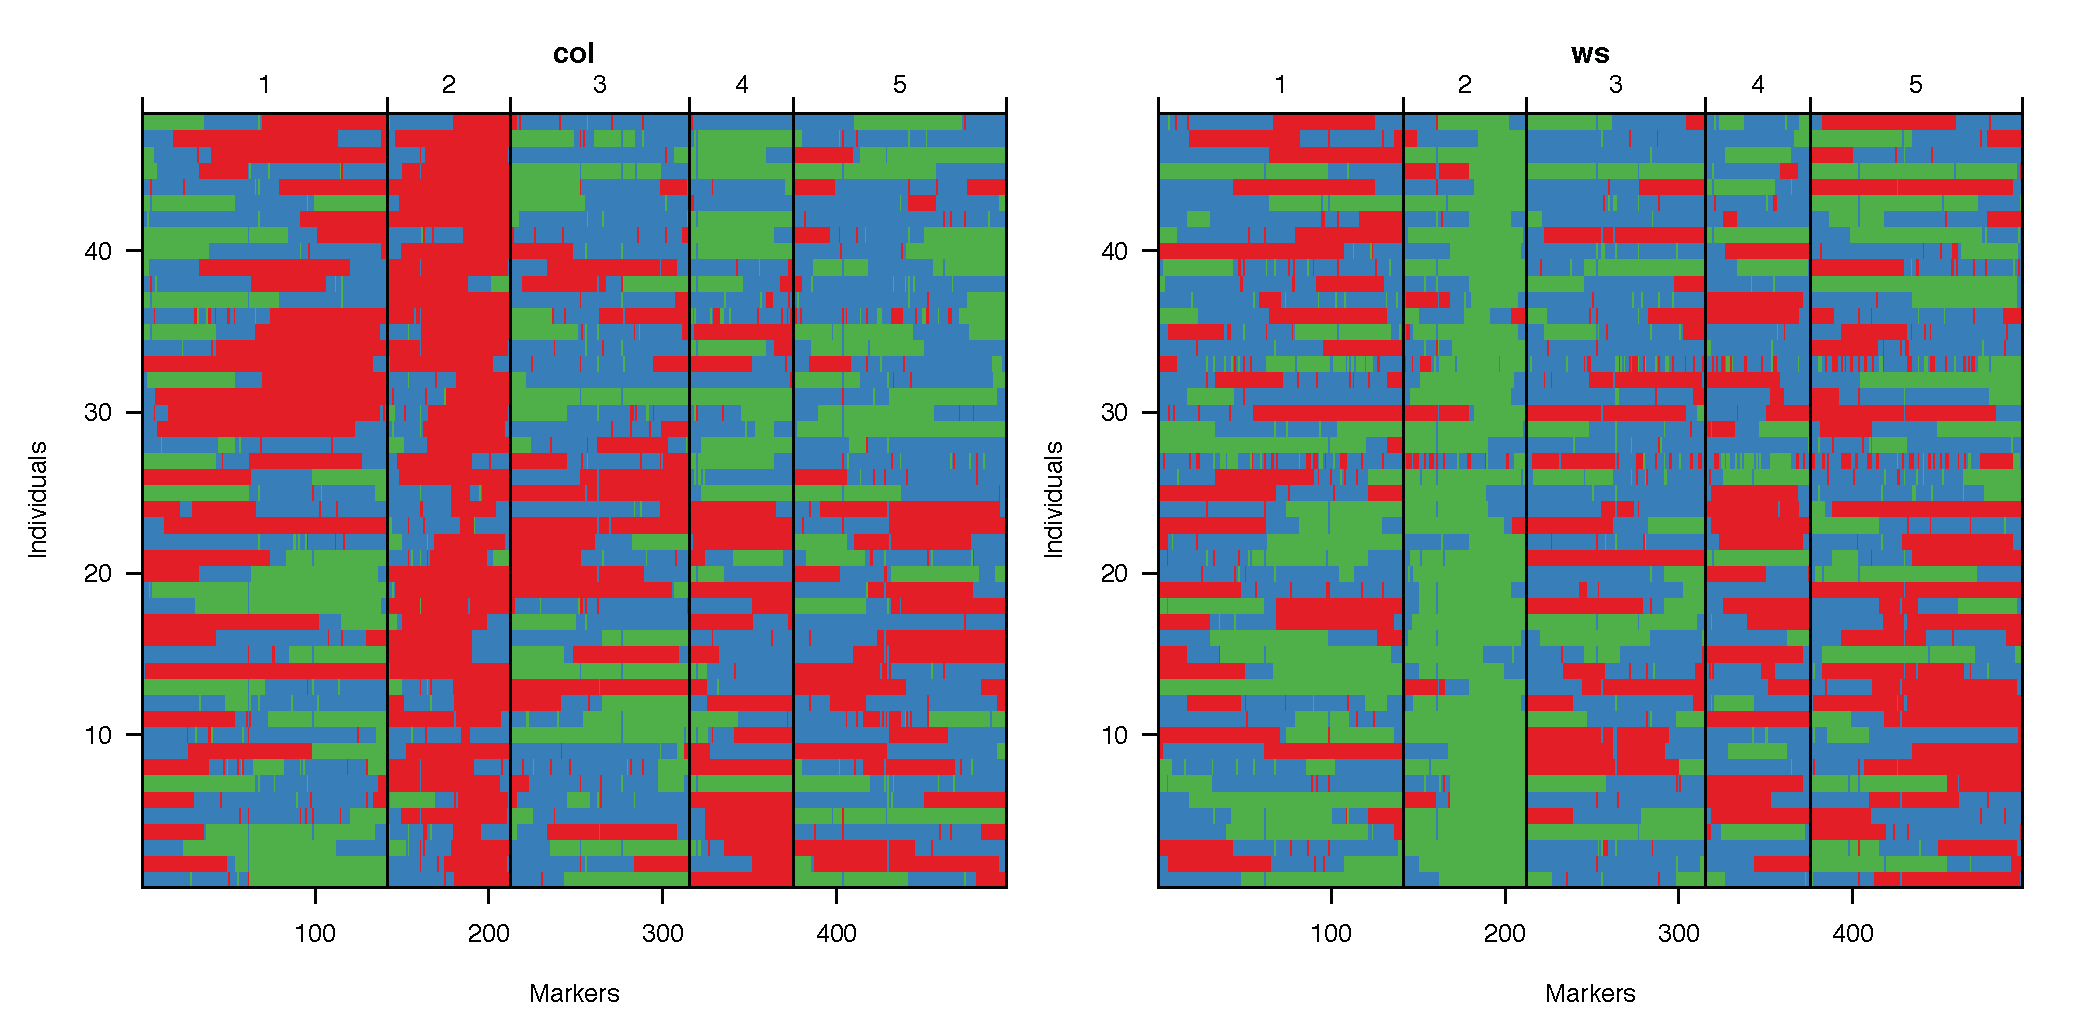
\includegraphics[width=6in]{elf3_epi/elf3_figs3_genoimage.pdf}
\caption[Genotypes of the 96 extreme $F_2$s used for sequencing.]{Genotypes of the 96 extreme $F_2$s used for sequencing. Sorted vertically by descending phenotype (longer hypocotyls above, shorter hypocotyls at bottom), chromosomes are displayed along the X axis. \emph{ELF3-Col} homozygotes at left, \emph{ELF3-Ws} homozygotes at right. Red indicates homozygosity for Col allele, blue indicates heterozygosity, and green indicates homozygosity for Ws allele.} \label{fig:app5fig3}
\end{figure}

\begin{figure}[H]
\graphicspath{{}}
\includegraphics[width=5.5in]{elf3_epi/stwo_qtl_022815.pdf}
\caption[2-locus QTL scan indicates potential genetic interactions between ELF3 and other loci.]{2-locus QTL scan indicates potential genetic interactions between ELF3 and other loci. Lower triangle indicates LOD for full model, upper triangle indicates LOD for interaction terms alone. \emph{ELF3} corresponds to the locus on chromosome 2.} \label{fig:app5fig4}
\end{figure}

\begin{figure}[H]
\graphicspath{{}}
\includegraphics[width=5in]{elf3_epi/elf3_interactionplots_031715-01.png}
\caption[Effect on hypocotyl length of various QTLs interacting with the ELF3 locus. ]{Effect on hypocotyl length of various QTLs interacting with the ELF3 locus. X-axis is non-ELF3 locus, different lines indicate effects of other locus in different ELF3 backgrounds. Error bars represent standard error of the mean.} \label{fig:app5fig5}
\end{figure}

\begin{figure}[H]
\graphicspath{{}}
\includegraphics[width=4in]{elf3_epi/elf3_figs6_candidates-01.pdf}
\caption[Analysis of 15d hypocotyl length under SD of candidate gene mutants.]{Analysis of 15d hypocotyl length under SD of candidate gene mutants. N ~ 50 for each line, each panel represents an independently conducted experiment, each repeated at least once with similar results. (A): 1 = Col WT, 2 = \emph{lsh9}, 3 = \emph{tsf}, 4 = \emph{elf3}, 5 = \emph{svl2}. Experiment was repeated with similar results. \emph{lsh9} is ~0.5 mm shorter (p = 0.03, t-test), \emph{elf3-200} is very elongated relative to WT (p < 2.2e-16, t-test). All others p > 0.1. N > 45 for each genotype. (B): Same as (A), but testing other candidates: 1 = \emph{soc1}, 2 = \emph{nup98}, 3 = \emph{cyct1;4}, 4 = Col WT, 5 = \emph{saur38}, \emph{arf1}, \emph{pif4-2}, \emph{elf3-200}. T-tests for differences vs. Col WT: p < 2.2e-16 for \emph{pif4} and \emph{elf3}; p = 0.009 for \emph{cyct1;4}, p = 0.033 for \emph{nup98}, p > 0.1 for all others. The \emph{cyct1;4} T-DNA insertion could not be confirmed by PCR and was thus omitted from further analysis. (C): Double mutant analysis of \emph{nup98} and \emph{elf3} does not indicate a genetic interaction. Error bars indicate standard deviation; N > 40 for each group; F-statistic and p-value are displayed for testing the hypothesis of an interaction between the two genes in controlling phenotype. } \label{fig:app5fig6}
\end{figure}

\begin{figure}[H]
\graphicspath{{}}
\includegraphics[width=3in]{elf3_epi/elf3_figsA_121515-01}
\caption[GAL4 DBD-ELF3 fusions do not lead to Y2H activation in combination with GAL4 AD-LSH9 vectors carrying either the Col or Ws variant of \emph{LSH9}.]{GAL4 DBD-ELF3 fusions do not lead to Y2H activation in combination with GAL4 AD-LSH9 fusions carrying either the Col or Ws variant of LSH9. Yeast carrying indicated vectors were spotted in five-fold dilutions onto C-leu-trp (C-LT) or C-leu-trp-his-ade (C-LTHA) media. For each protein X, experiments were repeated with independent PJ69-4$\alpha$ + pGADT7-X transformants with similar results.} \label{fig:app5fig7}
\end{figure}

\begin{figure}[H]
\graphicspath{{}}
\includegraphics[width=1.5in]{elf3_epi/elf3_figself3expr_lsh9_022516-01}
\caption[\emph{ELF3} expression is not substantially affected by \emph{lsh9} T-DNA insertion.]{\emph{ELF3} expression is not substantially affected by \emph{lsh9} T-DNA insertion. ELF3 expression was measured by PCR and normalized to \emph{UBC21} expression (Col set to 1.0). Error bars are standard error of the mean from three technical replicates. This experiment was repeated with similar results.} \label{fig:app5fig8}
\end{figure}


\begin{figure}[H]
\graphicspath{{}}
\includegraphics[width=4in]{elf3_epi/elf3_supp_emptyy2h_121015-01}
\caption[The GAL4 DBD-ELF3 fusion does not autoactivate in combination with a GAL4 AD-empty vector (pGADT7).]{The GAL4 DBD-ELF3 fusion does not autoactivate in combination with a GAL4 AD-empty vector (pGADT7). Yeast carrying indicated vectors were spotted in five-fold dilutions onto C-leu-trp (C-LT) or C-leu-trp-his-ade (C-LTHA) media. This experiment was repeated with an independent PJ69-4$\alpha$ + pGADT7 transformant with similar results.} \label{fig:app5fig9}
\end{figure}

\begin{figure}[H]
\graphicspath{{}}
\includegraphics[width=5.5in]{elf3_epi/elf3_figsZZZ_pif4fail_121415-01}
\caption[ELF3-PIF4 interaction not detectable in our assay.]{ELF3-PIF4 interaction not detectable in our assay. Row labels of strains correspond to contents of pGBK vector expressing GAL4 DBD fusions. Label at right indicates GAL4 AD fusion expressed in strains. (A): Assays in PJ69-4? strain background, (B): Assays in Y187 strain background. C-LT: YC-leu-trp media, C-LTH: YC-leu-trp-his media, YC-leu-trp-his-ade media. Y187 background showed activation with BD-ELF3 and AD-ELF4 and AD-PHYB (data not shown), but only on C-LTH. For each protein X, experiments were repeated with independent PJ69-4?/Y187 + pGADT7-PIF4 transformants with similar results.} \label{fig:app5fig10}
\end{figure}

\begin{figure}[H]
\graphicspath{{}}
\includegraphics[width=5in]{elf3_epi/lacz_assay_results_22hr_012216.pdf}
\caption[X-gal cleavage assay confirms modest differences in affinity between ELF3-polyQ variants for various proteins in Y2H.]{X-gal cleavage assay confirms modest differences in affinity between ELF3-polyQ variants for various proteins in Y2H. Bar labels indicate the GAL4 DNA binding domain construct, either empty or containing \emph{ELF3} with various polyQ-expressing lengths. In each assay, all observations are expressed relative to the activity of the empty vector, whose mean is set to 0. Error bars indicate standard deviation across three technical replicates. This experiment was repeated with similar results.} \label{fig:app5fig11}
\end{figure}

\section{Supporting Tables}

\begin{table}
\scriptsize
\caption{Primers employed in this study.\label{tab:app5tab1}} 
\begin{tabular}{|c c c|}
\hline
Primer name & target & sequence \\
\hline
nga111\_F & chr1 mapping & TGTTTTTTAGGACAAATGGCG \\
nga111\_R & chr1 mapping & CTCCAGTTGGAAGCTAAAGGG \\
nga280\_F & chr1 mapping & GGCTCCATAAAAAGTGCACC \\
nga280\_R & chr1 mapping & CTGATCTCACGGACAATAGTGC \\
nga168\_f & chr2 mapping & GAGGACATGTATAGGAGCCTCG \\
nga168\_R & chr2 mapping & TCGTCTACTGCACTGCCG \\
1H1L-1.6\_F & chr4 mapping & CTAGAGCTTGAAAGTTGATG \\
1H1L-1.6\_R & chr4 mapping & TTGAGTCCTTCTTGTCTG \\
g3883-1.4\_F & chr4 mapping & TGTTTCAGAGTAGCCAATTC \\
g3883-1.4\_R & chr4 mapping & CATCCATCAAACAAACTCC \\
nga129\_F & chr5 mapping & CACACTGAAGATGGTCTTGAGG \\
nga129\_R & chr5 mapping & TCAGGAGGAACTAAAGTGAGGG \\
rps4\_NT\_R & chr5 mapping & GGTACCTTTTCTTGTCAATG \\
rps4-NT\_F & chr5 mapping & TCATCAATTTCCGTGGGGCA \\
cyct1;4 tdna F & cyct1;4 & CTTTCCATTTTTCTCTTCCGG \\
cyct1;4 tdna R & cyct1;4 & TGGAATTTTGTTAACGATGGG \\
ELF3 STR F & ELF3 & CCCTTC CCATGG GATTCCCACCTCCTGGTAAT \\
ELF3 STR R & ELF3 & TTTTGGGGCGCC GGTTCATTATCAGATCTCTG \\
ELF3 clone F & ELF3 & AG GCC GAA TTC CCG GGG ATG AAG AGA GGG AAA GA \\
ELF3 clone R & ELF3 & G CAG GTC GAC GGATCC TTA AGG CTT AGA GGA GTC ATA GCG \\
ELF4 clone f & ELF4 & G GAG GCC AGT GAATTC ATG AAG AGG AAC GGC GAG ACG AAA \\
ELF4 clone r & ELF4 & C ATC TGC AG CAT ATG C TTA AGC TCT AGT TCC GGC AGC ACC \\
lsh9 clone f & lsh9 & G GAG GCC AGT GAATTC ATGTCTTCGGATCGTCACACACC \\
lsh9 clone r & lsh9 & C ATC TGC AG C TCG AGC TCAAGTGAACGACTGATTAGGAG \\
lsh9\_expr\_f & LSH9 & CGGGTTCACTTGAGGGAAGTG \\
lsh9-1 genotype\_r & LSH9 & CAAGTGAACGACTGATTAGGAGT \\
lsh9-1 genotype\_f & LSH9 & TTTTCGTGAATAATTCTCTCTCCC \\
nup98 tdna f & nup98 & TTTTCTGAATTTTGGCTTTGTCTT \\
nup98 tdna r & nup98 & AGTCTACACACATCCGTCTCTCCT/AGTCTACACACATCCGTCTCT \\
matchmaker insert F & plasmid insert & TCA TCG GAA GAG AGT AG  \\
matchmaker insert R & plasmid insert &  GTCACTTTAAAATTTGTATAC \\
\end{tabular}
\end{table}
\begin{table}
\scriptsize
\begin{tabular}{|c c c|}
phyb\_ clone f & phyb & GGAGGCCAGTCATATGATTGATGAGTTAGGTGCAGTTG \\
phyb\_ clone r & phyb & CATCTGCAGGGATCCCCTAATATGGCATCATCAGCATCAT \\
pif4  clone f & pif4 & GGAGGCCAGTGAATTCATGGAACACCAAGGTTGGAGTTTT \\
pif4  clone r & pif4 & C ATC TGC AG C TCG AGC CTAGTGGTCCAAACGAGAACCGTC \\
pif4-2 genotyping f & pif4 & ACCTCCTCAAGTCATGGTTAAGCCTAAGCC \\
pif4-2 genotyping r & pif4 & TCCAAACGAGAACCGTCGGT \\
saur38 tdna f & saur38 & GATGGTTAGATCAATGGGCTG \\
saur38 tdna r & saur38 & CCCCGATTCTCAATATTCACC \\
soc1 tdna f & soc1 & AAGGATGAGGTTTCAAGCGTC \\
soc1 tdna r & soc1 & TGGCGAATTCATAAAGTTTGC \\
svl2-1 T-DNA & svl2 & GAGTGTGCATTTGTGTGAAG \\
svl2-1 T-DNA & svl2 & ACGATGCGTTCTATGAGCAA \\
pif4-2 & T-DNA & TAGCATCTGAATTTCATAACCAATCTCGATACAC \\
lsh9-1 & T-DNA & ATAATAACGCTGCGGACATCTACATTTT \\
tsf-1 lp & TSF & CGGTTAACTTGATTTTGTTTC \\
tsf-1 rp & TSF & ACGTGGACTCTCGTAGCACA \\
UBC21 expression f & UBC21 & GACCAAGATATTCCATCCTA \\
UBC21 expression r & UBC21 & GTTAAGAGGACTGTCCG \\
\hline
\end{tabular}
\end{table}

\begin{table}
\caption{Mutant lines employed in this study.\label{tab:app5tab2}} 
\begin{tabular}{|c c|}
\hline
mutant & identifier \\
\hline
soc1 (Col-0): & SALK\_138131C \\
nup98 (Col-0): &  CS2103568 = GK-288A08-015346  \\
arf1-3 (Col-0): & CS24599 \\
pif4-2 (Col-0): & CS66043 \\
saur38 (Col-0): &  SALK\_001155 \\
cyct1;4 (Col-0): & SALK\_139322 \\
lsh9 (Col-0) & CS328437 \\
tsf (Col-0) & SALK\_087522C \\
elf3-200 (Col) & GABI750E02 \\
elf3-4 (Ws) & CS3790 \\
svl2 (Col) & SALK\_057865 \\
\hline
\end{tabular}
\end{table}

\begin{table}
\scriptsize
\caption{Col x Ws segregants analyzed by genotyping-by-sequencing.\label{tab:app5tab3}} 
\begin{tabular}{|c c c c c c c c c|}
\hline
Barcode & genome & plate & plate & d15 hypocotyl & transplant & row & column & ELF3 Col \\
 & coverage & number &  position & length & tray &(A-F) & (1-12) & alleles \\
\hline
GACTTCGTA & 1.93 & 5 & 1 & 5.669 & BOTTOM1 & A & 7 & 0 \\
AATCTCGTC & 2.15 & 5 & 2 & 6.127 & BOTTOM1 & A & 8 & 0 \\
TCTTACGGT & 2.8 & 5 & 4 & 11.236 & TOP1 & B & 2 & 2 \\
TTGCCACTA & 1.98 & 5 & 5 & 9.591 & TOP1 & B & 3 & 0 \\
GCGTTAATG & 2.99 & 5 & 10 & 11.24 & TOP1 & B & 4 & 2 \\
CTTCAACGA & 1.13 & 6 & 9 & 7.457 & BOTTOM4 & A & 6 & 2 \\
AGCGTACTA & 1.72 & 7 & 5 & 11.136 & TOP1 & B & 7 & 2 \\
TGATCTGAG & 5.22 & 8 & 4 & 9.95 & TOP1 & B & 8 & 0 \\
TACGGTGAA & 2.02 & 10 & 6 & 9.611 & TOP1 & B & 11 & 0 \\
ATGCATGAC & 2.22 & 10 & 9 & 9.539 & TOP1 & B & 12 & 0 \\
AACTGTCCT & 2.31 & 11 & 3 & 6.543 & BOTTOM1 & B & 11 & 0 \\
AGACACCAT & 2.82 & 11 & 5 & 6.15 & BOTTOM1 & B & 12 & 2 \\
AGAACATCC & 1.58 & 14 & 5 & 6.347 & BOTTOM1 & C & 8 & 0 \\
CTGGATAAG & 1.69 & 16 & 4 & 6.33 & BOTTOM1 & D & 3 & 0 \\
GTGACTTAC & 3.22 & 17 & 7 & 6.014 & BOTTOM1 & D & 6 & 0 \\
CTCACTGAA & 0.89 & 18 & 7 & 10.985 & TOP1 & C & 9 & 2 \\
TGAGACATG & 1.88 & 19 & 2 & 7.147 & BOTTOM1 & D & 10 & 2 \\
TCCACGATT & 2.96 & 19 & 3 & 11.082 & TOP1 & C & 10 & 2 \\
GACTGATAC & 1.38 & 20 & 1 & 6.238 & BOTTOM1 & D & 11 & 0 \\
ACATCTGCT & 2.27 & 22 & 5 & 11.093 & TOP1 & D & 2 & 2 \\
ACGTTAGGA & 2.81 & 25 & 1 & 6.038 & BOTTOM1 & E & 9 & 0 \\
TGGACTGTT & 2.56 & 25 & 2 & 7.366 & BOTTOM1 & E & 10 & 2 \\
TTCTCAAGG & 3.43 & 26 & 2 & 10.628 & TOP1 & D & 9 & 0 \\
CAGGCTTAA & 1.99 & 26 & 8 & 5.687 & BOTTOM1 & E & 11 & 0 \\
GTGGTCTAA & 1.65 & 27 & 5 & 6.623 & BOTTOM1 & F & 2 & 2 \\
CACTAGACA & 1.44 & 27 & 7 & 6.099 & BOTTOM1 & F & 3 & 0 \\
CTCGATCTA & 1.97 & 27 & 8 & 5.841 & BOTTOM1 & F & 4 & 0 \\
TGGCATTCA & 2.45 & 28 & 8 & 7.356 & BOTTOM1 & F & 7 & 2 \\
ACATTGCAC & 0.13 & 29 & 10 & 10.164 & TOP1 & E & 3 & 0 \\
TATGCCACT & 1.66 & 30 & 9 & 9.948 & TOP1 & E & 7 & 0 \\
ACCGATCAT & 1.36 & 34 & 4 & 6.036 & BOTTOM2 & A & 2 & 0 \\
AGGTAGACT & 2.83 & 34 & 8 & 7.093 & BOTTOM2 & A & 3 & 2 \\
\end{tabular}
\end{table}
\begin{table}
\scriptsize
\begin{tabular}{|c c c c c c c c c|}
CAGTTGATC & 3.27 & 35 & 8 & 13.69 & TOP1 & E & 11 & 2 \\
ACTACCGAT & 0.33 & 36 & 7 & 6.536 & BOTTOM2 & A & 8 & 0 \\
CATCATACG & 0.38 & 36 & 8 & 6.947 & BOTTOM2 & A & 9 & 2 \\
CGTCAGTAA & 2.22 & 37 & 5 & 6.455 & BOTTOM2 & A & 10 & 0 \\
TTACGACAG & 3.85 & 37 & 6 & 11.178 & TOP1 & F & 6 & 2 \\
ACCAGTTGA & 2.2 & 38 & 2 & 11.28 & TOP1 & F & 7 & 2 \\
GAGATCGAT & 2.5 & 38 & 5 & 10.384 & TOP1 & F & 8 & 0 \\
CATAGTTGC & 1.49 & 39 & 8 & 9.551 & TOP1 & F & 11 & 0 \\
GAAGTCATC & 1.04 & 41 & 3 & 7.123 & BOTTOM2 & B & 4 & 2 \\
TGTAACGTC & 0.34 & 42 & 3 & 9.333 & TOP4 & D & 12 & 0 \\
TAGCAGATG & 0.52 & 43 & 2 & 11.533 & TOP2 & A & 5 & 2 \\
CCGACTAAT & 1.89 & 44 & 4 & 7.572 & BOTTOM4 & E & 7 & 2 \\
AGTACGCTA & 5.31 & 47 & 5 & 7.401 & BOTTOM4 & F & 1 & 2 \\
ATTGCTTGG & 1.25 & 52 & 3 & 11.307 & TOP2 & B & 10 & 2 \\
CAATTACGG & 3.12 & 52 & 6 & 11.585 & TOP2 & B & 11 & 0 \\
GGCAATTCT & 2.86 & 53 & 9 & 11.33 & TOP2 & C & 4 & 2 \\
GTTACAGGT & 2.43 & 54 & 4 & 7.08 & BOTTOM2 & C & 11 & 2 \\
ACACTGATG & 1.65 & 54 & 10 & 7.558 & BOTTOM4 & F & 11 & 2 \\
TGAGGATTC & 0.06 & 55 & 3 & 11.25 & TOP2 & C & 7 & 2 \\
GTATACAGC & 1.64 & 55 & 6 & 11.276 & TOP2 & C & 8 & 2 \\
ATAGCCTTC & 1.28 & 56 & 9 & 13.121 & TOP2 & C & 11 & 2 \\
ATCGATTCC & 0.3 & 57 & 8 & 11.378 & TOP2 & D & 2 & 0 \\
ACCATAAGC & 1.08 & 60 & 10 & 11.106 & TOP2 & D & 8 & 2 \\
AATGCGTCA & 1.84 & 62 & 3 & 5.465 & BOTTOM2 & D & 9 & 2 \\
AGAATCGTG & 3.76 & 63 & 1 & 11.802 & TOP2 & D & 12 & 2 \\
GAGGCAATA & 5.49 & 63 & 2 & 6.727 & BOTTOM2 & D & 10 & 2 \\
CTCTGACTT & 2.38 & 63 & 7 & 7.325 & BOTTOM2 & D & 12 & 2 \\
CTCAGCTAT & 1.82 & 64 & 10 & 7.492 & BOTTOM5 & B & 1 & 2 \\
TTGTGAGCA & 0.67 & 66 & 1 & 11.79 & TOP2 & E & 6 & 2 \\
TCAGAAGAC & 2.59 & 66 & 8 & 9.554 & TOP2 & E & 10 & 0 \\
\end{tabular}
\end{table}
\begin{table}
\scriptsize
\begin{tabular}{|c c c c c c c c c|}
AATCGGCAA & 2.85 & 68 & 1 & 6.247 & BOTTOM2 & F & 1 & 0 \\
GTATTCGAG & 2.04 & 71 & 2 & 7.447 & BOTTOM5 & B & 5 & 2 \\
TAGAAGCCA & 0.96 & 72 & 2 & 5.903 & BOTTOM2 & F & 10 & 0 \\
AATGGCCTT & 0.06 & 72 & 4 & 7.5 & BOTTOM5 & B & 7 & 2 \\
GGTCAACTT & 1.28 & 72 & 7 & 9.469 & TOP5 & B & 7 & 0 \\
TCAGTTCAG & 1.65 & 74 & 6 & 6.274 & BOTTOM3 & A & 1 & 0 \\
TACACCTAG & 3.86 & 75 & 5 & 11.728 & TOP3 & A & 3 & 2 \\
CTAAGATGG & 2.43 & 76 & 7 & 6.275 & BOTTOM3 & A & 4 & 0 \\
ATGTCGTAG & 2.72 & 79 & 1 & 11.183 & TOP3 & A & 11 & 0 \\
CATGTTGGA & 2.37 & 83 & 10 & 10.927 & TOP3 & B & 12 & 2 \\
GATGATAGC & 1.34 & 84 & 10 & 7.129 & BOTTOM3 & B & 6 & 2 \\
TGAAGCTGT & 0.41 & 85 & 3 & 9.945 & TOP3 & C & 3 & 0 \\
GCAATGACT & 2.41 & 86 & 7 & 7.122 & BOTTOM3 & B & 8 & 2 \\
TCGAGATCT & 0.07 & 88 & 1 & 6.308 & BOTTOM3 & B & 10 & 2 \\
CAAGAGCAT & 4.01 & 89 & 6 & 9.568 & TOP3 & C & 8 & 0 \\
ACGCACTAA & 1.97 & 91 & 6 & 11.414 & TOP3 & C & 9 & 2 \\
GAACTAGGA & 1.12 & 92 & 9 & 10.626 & TOP3 & D & 2 & 0 \\
TAATGCACC & 1.74 & 92 & 10 & 9.545 & TOP3 & D & 3 & 0 \\
ATCCTCAGT & 0.48 & 93 & 5 & 9.986 & TOP3 & D & 4 & 0 \\
TGACTGCTA & 2.89 & 93 & 8 & 9.61 & TOP3 & D & 5 & 0 \\
TTCGAGTGA & 0.57 & 94 & 4 & 12.438 & TOP3 & D & 8 & 2 \\
CTGATTGGT & 2.16 & 94 & 5 & 9.509 & TOP3 & D & 9 & 0 \\
GTCCATATC & 2.36 & 94 & 7 & 5.843 & BOTTOM3 & C & 6 & 0 \\
GATCTCTCA & 1.59 & 95 & 1 & 6.764 & BOTTOM3 & C & 7 & 2 \\
CTAATGGCA & 0.14 & 103 & 5 & 6.028 & BOTTOM3 & D & 8 & 0 \\
TGCGTTAGT & 1.13 & 103 & 7 & 9.381 & TOP5 & F & 1 & 0 \\
ATATCGACC & 0.98 & 105 & 3 & 13.88 & TOP3 & E & 12 & 2 \\
ATAACTCGC & 1.14 & 107 & 7 & 6.881 & BOTTOM3 & E & 7 & 2 \\
TACTCAGTC & 3.62 & 108 & 5 & 6.35 & BOTTOM3 & E & 9 & 0 \\
GGAGTATCT & 2.28 & 109 & 1 & 6.465 & BOTTOM3 & E & 10 & 0 \\
AACTCTAGC & 2.9 & 109 & 10 & 9.839 & TOP3 & F & 9 & 0 \\
CGCTACATT & 3.27 & 110 & 5 & 10.838 & TOP3 & F & 10 & 2 \\
CATTACGAG & 2.16 & 111 & 1 & 5.796 & BOTTOM3 & F & 4 & 0 \\
GTGCTACAT & 1.39 & 113 & 2 & 6.032 & BOTTOM3 & F & 12 & 0 \\
\hline
\end{tabular}
\end{table}

\begin{table}
\caption{Multiple QTL mapping results.\label{tab:app5tab4}} 
\begin{tabular}{|c c c c|}
\hline
Chromosome & Position & 90\% credible interval & LOD \\
\hline
Raw model &   &   &   \\
\hline
1 & 23265613 & (18260614 : 25453225) & 3.3 \\
2 & 9920153 & (5758889 : 18882167) & 3.01 \\
4 & 10199204 & (6295201 : 15296654) & 2.83 \\
5 & 18703510 & (9072000 : 26544677) & 2.61 \\
\hline
Refined model (from MQM) &   &   &   \\
\hline
1 & 1,589,277 & (292344 : ~30,000,000) & 14.5 \\
2 & 10,906,049 & (10906049 : 11063324) & 17.03 \\
2 & 13,973,428 & (11822190: ~17,000,000) & 5.12 \\
4 & ~10,000,000 & (8873411 : 11578413) & 8.27 \\
5 & 18,184,159 & (~17,600,000 : 19470953) & 7.05 \\
\hline
\end{tabular}
\end{table}

\chapter{Supporting Chapter 6}
\section{Supporting Figures}
\begin{figure}[H]
\graphicspath{{}}
\includegraphics[width=5in]{elf3temp_pgen_sub/FigS1.png}
\caption[Expression analysis of \emph{PIF4} and \emph{AtHB2} depends on temperature, genetic background, and ELF3 functionality.]{Expression analysis of \emph{PIF4} and \emph{AtHB2} depends on temperature, genetic background, and ELF3 functionality. Error bars represent the standard error of the mean across 3 technical replicates. White bars represent 22$\degree$ expression, red bars 27$\degree$ expression for each line. Tissue was collected from 7d seedlings at ZT0. This experiment was repeated with similar results.} \label{fig:app6fig1}
\end{figure}
\begin{figure}[H]
\graphicspath{{}}
\includegraphics[width=5in]{elf3temp_pgen_sub/FigS2.png}
\caption[Regulation of adult thermoresponsive traits by ELF3 and FCA is independent of PIF4 and modulated by genetic background.]{Regulation of adult thermoresponsive traits by ELF3 and FCA is independent of PIF4 and modulated by genetic background. Flowering temperature response of indicated genotypes under indicated conditions, measured by rosette leaf number (RLN) at flowering. For each experiment, n > 10 plants for each genotype in each treatment. Regression analysis of data in Tables ~\ref{tab:app6tab4}, ~\ref{tab:app6tab5}.} \label{fig:app6fig2}
\end{figure}
\section{Supporting Tables}
\begin{table}[H]
\caption[Regression analysis of hypocotyl elongation temperature response among Col and Ws transgenic lines.]{Regression analysis of hypocotyl elongation temperature response among Col and Ws transgenic lines. \label{tab:app6tab1}}
\begin{tabular}{| c c c c c |}
\hline
Group & Estimate & Std. Error & t value & Pr(>|t|) \\
\hline
Col model & & & & \\
\hline
Col, 22d (Intercept) & 6.93 & 0.29 & 24.14 & 2.04E-97 \\
elf3 & 5.81 & 0.36 & 16.29 & 7.97E-52 \\
Col\_0R & 5.59 & 0.35 & 15.75 & 5.67E-49 \\
Col\_16R & 6.24 & 0.35 & 17.58 & 7.76E-59 \\
Col\_20R & 3.51 & 0.41 & 8.63 & 3.18E-17 \\
Col\_23R & 4.8 & 0.37 & 13.14 & 6.86E-36 \\
Col\_7R & 3.22 & 0.41 & 7.86 & 1.20E-14 \\
Col\_9R & 3.85 & 0.39 & 9.82 & 1.37E-21 \\
27 degree treatment & 2.78 & 0.38 & 7.28 & 7.91E-13 \\
Experiment 2 & 0.61 & 0.12 & 5.01 & 6.74E-07 \\
27d : elf3 & -2.93 & 0.47 & -6.2 & 9.01E-10 \\
27d : Col\_0R & -2.63 & 0.48 & -5.53 & 4.32E-08 \\
27d : Col\_7R & -2.63 & 0.47 & -5.59 & 3.14E-08 \\
27d : Col\_9R & -0.79 & 0.55 & -1.42 & 0.16 \\
27d : Col\_16R & -2.02 & 0.48 & -4.19 & 3.05E-05 \\
27d : Col\_20R & -1.49 & 0.54 & -2.74 & 0.0062 \\
27d : Col\_23R & -2.44 & 0.52 & -4.72 & 2.79E-06 \\
\hline
\end{tabular}
\end{table}
\begin{table}
\begin{tabular}{| c c c c c |}
Ws model & & & & \\
\hline
Ws 22degree (Intercept) & 5.99 & 0.31 & 19.64 & 5.76E-70 \\
elf3 & 9.27 & 0.37 & 24.75 & 4.56E-100 \\
Ws\_0R & 6.48 & 0.41 & 15.71 & 1.81E-48 \\
Ws\_7R & 5.57 & 0.39 & 14.3 & 2.52E-41 \\
Ws\_9R & -0.31 & 0.52 & -0.59 & 0.55 \\
Ws\_16R & 3.93 & 0.43 & 9.17 & 4.34E-19 \\
Ws\_20R & 4.83 & 0.38 & 12.64 & 2.06E-33 \\
Ws\_23R & 6.97 & 0.4 & 17.52 & 3.78E-58 \\
27 degree treatment & 3.27 & 0.41 & 7.9 & 9.26E-15 \\
Experiment 2 & 0.46 & 0.14 & 3.37 & 0.00079 \\
27d : elf3 & -4.38 & 0.51 & -8.67 & 2.55E-17 \\
27d : Ws\_0R & -3.56 & 0.55 & -6.51 & 1.39E-10 \\
27d : Ws\_7R & -3.4 & 0.52 & -6.53 & 1.20E-10 \\
27d : Ws\_9R & 0.23 & 0.67 & 0.35 & 0.73 \\
27d : Ws\_16R & -1.5 & 0.6 & -2.51 & 0.012 \\
27d : Ws\_20R & -3 & 0.52 & -5.78 & 1.06E-08 \\
27d : Ws\_23R & -2.52 & 0.53 & -4.74 & 2.54E-06 \\
\hline
\end{tabular}
\end{table}

\begin{table}[H]
\caption[Regression analysis of petiole : leaf length ratio and rosette leaf number at flowering temperature response among Col and Ws transgenic lines.]{Regression analysis of petiole : leaf length ratio and rosette leaf number at flowering temperature response among Col and Ws transgenic lines. \label{tab:app6tab2}}
\begin{tabular}{| c c c c c |}
\hline
Variable & Estimate & Std. Error & t value & Pr(>|t|) \\
\hline
Col model, PL:LL & & & & \\
Col, 22d (Intercept) & 0.47 & 0.01 & 58.2 & 7.72E-274 \\
27d treatment & 0.24 & 0.01 & 22.86 & 2.66E-87 \\
Col\_0R & 0.01 & 0.01 & 0.68 & 0.49 \\
Col\_16R & 0 & 0.01 & -0.19 & 0.85 \\
Col\_20R & 0 & 0.01 & 0.32 & 0.75 \\
Col\_23R & 0.01 & 0.01 & 0.6 & 0.55 \\
Col\_7R & 0 & 0.01 & -0.11 & 0.91 \\
Col\_9R & 0.01 & 0.01 & 0.52 & 0.6 \\
elf3 & 0 & 0.01 & -0.2 & 0.84 \\
Experiment 2 & -0.02 & 0.01 & -3.73 & 0.0002 \\
Experiment 3 & -0.08 & 0.01 & -11.95 & 3.86E-30 \\
27d : Col\_0R & 0.05 & 0.02 & 2.92 & 0.0037 \\
27d : Col\_16R & 0.06 & 0.02 & 2.99 & 0.0029 \\
27d : Col\_20R & 0.04 & 0.02 & 2.74 & 0.0064 \\
27d : Col\_23R & 0.02 & 0.02 & 1.17 & 0.24 \\
27d : Col\_7R & 0.05 & 0.02 & 2.95 & 0.0033 \\
27d : Col\_9R & 0.06 & 0.02 & 3.61 & 0.00033 \\
27d : elf3 & 0.08 & 0.02 & 5.11 & 4.17E-07 \\
\hline
\end{tabular}
\end{table}
\begin{table}
\begin{tabular}{| c c c c c |}
\hline
Ws model, PL:LL & & & & \\
\hline
Ws 22d (Intercept) & 0.47 & 0.01 & 54.96 & 3.68E-258 \\
27d treatment & 0.21 & 0.01 & 18.82 & 1.97E-64 \\
elf3 & -0.02 & 0.01 & -1.68 & 0.093 \\
Ws\_0R & -0.01 & 0.01 & -0.97 & 0.33 \\
Ws\_7R & -0.06 & 0.01 & -5.21 & 2.45E-07 \\
Ws\_9R & -0.01 & 0.01 & -0.88 & 0.38 \\
Ws\_16R & -0.01 & 0.01 & -1.1 & 0.27 \\
Ws\_20R & 0.02 & 0.01 & 1.46 & 0.14 \\
Ws\_23R & 0.01 & 0.01 & 0.6 & 0.55 \\
Experiment 2 & -0.04 & 0.01 & -5.88 & 6.35E-09 \\
Experiment 3 & -0.08 & 0 & -16.48 & 6.09E-52 \\
27d : elf3 & 0.1 & 0.02 & 6.28 & 5.83E-10 \\
27d : Ws\_0R & 0.04 & 0.02 & 2.79 & 0.0053 \\
27d : Ws\_7R & 0.09 & 0.02 & 5.6 & 3.12E-08 \\
27d : Ws\_9R & -0.01 & 0.02 & -0.37 & 0.71 \\
27d : Ws\_16R & 0.05 & 0.01 & 3.29 & 0.001 \\
27d : Ws\_20R & 0.09 & 0.02 & 5.31 & 1.47E-07 \\
27d : Ws\_23R & 0.06 & 0.02 & 3.72 & 0.00022 \\
\hline
\end{tabular}
\end{table}
\begin{table}
\begin{tabular}{| c c c c c |}
\hline
Col model, RLN at flowering & & & & \\
\hline
Col 22d (Intercept) & 14.31 & 0.22 & 63.71 & 3.08E-297 \\
27d treatment & -3.08 & 0.3 & -10.33 & 2.08E-23 \\
Col\_0R & -3.6 & 0.32 & -11.25 & 3.88E-27 \\
Col\_16R & -5.83 & 0.39 & -14.82 & 1.52E-43 \\
Col\_20R & -4.31 & 0.31 & -14 & 1.60E-39 \\
Col\_23R & -5.26 & 0.34 & -15.52 & 4.78E-47 \\
Col\_7R & -3.2 & 0.34 & -9.45 & 4.89E-20 \\
Col\_9R & -4.64 & 0.35 & -13.39 & 1.24E-36 \\
elf3 & -5.57 & 0.29 & -18.94 & 3.85E-65 \\
Experiment 2 & -1.66 & 0.14 & -11.71 & 4.36E-29 \\
Experiment 3 & -2.26 & 0.17 & -12.94 & 1.47E-34 \\
27d : Col\_0R & 2.32 & 0.45 & 5.2 & 2.62E-07 \\
27d : Col\_16R & 2.95 & 0.56 & 5.29 & 1.61E-07 \\
27d : Col\_20R & 2.53 & 0.45 & 5.57 & 3.66E-08 \\
27d : Col\_23R & 2.65 & 0.48 & 5.56 & 3.76E-08 \\
27d : Col\_7R & 1.68 & 0.48 & 3.51 & 0.00047 \\
27d : Col\_9R & 2.73 & 0.48 & 5.67 & 2.08E-08 \\
27d : elf3 & 2.79 & 0.42 & 6.63 & 6.58E-11 \\
\hline
\end{tabular}
\end{table}
\begin{table}
\begin{tabular}{| c c c c c |}
\hline
Ws model, RLN at flowering & & & & \\
\hline
Ws 22d (Intercept) & 6.87 & 0.18 & 38.09 & 5.77E-174 \\
27d treatment & 0.4 & 0.23 & 1.73 & 0.083 \\
elf3 & -1.23 & 0.23 & -5.29 & 1.63E-07 \\
Ws\_0R & -0.98 & 0.23 & -4.17 & 3.37E-05 \\
Ws\_7R & -1.35 & 0.25 & -5.36 & 1.14E-07 \\
Ws\_9R & 1.1 & 0.29 & 3.81 & 0.00015 \\
Ws\_16R & -0.24 & 0.23 & -1.05 & 0.29 \\
Ws\_20R & 2.19 & 0.26 & 8.46 & 1.47E-16 \\
Ws\_23R & -1.72 & 0.24 & -7.27 & 9.57E-13 \\
Experiment 2 & -0.38 & 0.13 & -2.89 & 0.0039 \\
Experiment 3 & -1.4 & 0.1 & -13.7 & 4.32E-38 \\
27d : elf3 & 0.43 & 0.33 & 1.31 & 0.19 \\
27d : Ws\_0R & 0.33 & 0.33 & 1 & 0.32 \\
27d : Ws\_7R & 0.12 & 0.34 & 0.34 & 0.74 \\
27d : Ws\_9R & -0.33 & 0.4 & -0.82 & 0.41 \\
27d : Ws\_16R & 0.41 & 0.32 & 1.3 & 0.2 \\
27d : Ws\_20R & -1.97 & 0.35 & -5.6 & 3.09E-08 \\
27d : Ws\_23R & 0.22 & 0.34 & 0.65 & 0.52 \\
\hline
\end{tabular}
\end{table}

\begin{table}[H]
\caption[Regression analysis of rosette leaf number at flowering and petiole : leaf length ratio temperature responses in \emph{elf3} and \emph{pif4}.]{Regression analysis of rosette leaf number at flowering and petiole : leaf length ratio temperature responses in \emph{elf3} and \emph{pif4}. \label{tab:app6tab3}}
\begin{tabular}{| c c c c c |}
\hline
Variable & Estimate & Std. Error & t value & Pr(>|t|) \\
\hline
RLN at flowering & & & & \\
Col 22d (Intercept) & 18.17 & 0.5 & 36.66 & 1.21E-58 \\
elf3 & -9.33 & 0.7 & -13.32 & 1.25E-23 \\
pif4 & -0.17 & 0.7 & -0.24 & 8.13E-01 \\
27\_14d & -6.17 & 0.7 & -8.8 & 5.21E-14 \\
27\_1d & -6.17 & 0.7 & -8.8 & 5.21E-14 \\
elf3:27d\_14d & 5.24 & 1 & 5.23 & 9.73E-07 \\
pif4:27d\_14d & 1.92 & 0.99 & 1.93 & 5.60E-02 \\
elf3:27d\_1d & 4.17 & 0.99 & 4.2 & 5.83E-05 \\
pif4:27d\_1d & 1.35 & 1 & 1.35 & 1.82E-01 \\
\hline
%\end{tabular}
%\end{table}
%\begin{table}
%\begin{tabular}{| c c c c c |}
\hline
25 DAY PL:LL & & & & \\
\hline
Col 22d (Intercept) & 0.48 & 0.01 & 46.17 & 7.79E-68 \\
elf3 & -0.02 & 0.01 & -1.43 & 0.16 \\
pif4 & -0.08 & 0.01 & -5.52 & 2.82E-07 \\
27d\_14day & 0.17 & 0.01 & 11.26 & 2.62E-19 \\
27d\_1day & 0.21 & 0.01 & 14.26 & 1.53E-25 \\
elf3:27d\_14day & 0.06 & 0.02 & 3 & 0.0034 \\
pif4:27d\_14day & -0.1 & 0.02 & -4.76 & 6.67E-06 \\
elf3:27d\_1day & 0.08 & 0.02 & 4.08 & 9.29E-05 \\
pif4:27d\_1day & -0.13 & 0.02 & -6.3 & 8.69E-09 \\
\hline
\end{tabular}
\end{table}

\begin{table}[H]
\caption[Regression analysis of rosette leaf number at flowering temperature response in Ws and \emph{elf3-4}.]{Regression analysis of rosette leaf number at flowering temperature response in Ws and \emph{elf3-4}. \label{tab:app6tab3}}
\begin{tabular}{| c c c c c |}
\hline
Variable & Estimate & Std. Error & t value & Pr(>|t|) \\
\hline
Ws 16d (Intercept) & 12.35 & 0.23 & 52.58 & 1.97E-45 \\
22d & -3.07 & 0.35 & -8.77 & 1.09E-11 \\
elf3-4 & -6.35 & 0.37 & -17.39 & 7.52E-23 \\
22d : elf3-4 & 2.79 & 0.53 & 5.23 & 3.37E-06 \\
\hline
\end{tabular}
\end{table}

\begin{table}[H]
\caption[Regression analysis of petiole : leaf length ratio temperature response in Col and \emph{fca} mutants.]{Regression analysis of petiole : leaf length ratio temperature response in Col and \emph{fca} mutants. \label{tab:app6tab4}}
\begin{tabular}{| c c c c c |}
\hline
Variable & Estimate & Std. Error & t value & Pr(>|t|) \\
\hline
Col 22d (Intercept) & 0.46 & 0.01 & 35.74 & 6.57E-45 \\
27d & 0.23 & 0.02 & 12.71 & 2.09E-19 \\
fca T-DNA & 0.01 & 0.02 & 0.3 & 0.77 \\
fca-9 & -0.03 & 0.02 & -1.68 & 0.098 \\
27d : fca T-DNA & -0.03 & 0.03 & -1.36 & 0.18 \\
27d : fca-9 & -0.02 & 0.03 & -0.82 & 0.41 \\
\hline
\end{tabular}
\end{table}

\begin{table}[H]
\caption[Regression analysis of rosette leaf number at flowering and petiole length temperature responses in \emph{elf3} and \emph{pif4} mutants under various treatments.]{Regression analysis of rosette leaf number at flowering and petiole length temperature responses in \emph{elf3} and \emph{pif4} mutants under various treatments. \label{tab:app6tab5}}
\begin{tabular}{| c c c c c |}
\hline
Variable & Estimate & Std. Error & t value & Pr(>|t|) \\
\hline
RLN at FLOWERING  & & & &\\
\hline
elf3-200 22d (Intercept) & 8.06 & 0.44 & 18.33 & 4.18E-37 \\
pif4-2 & 8.61 & 0.61 & 14.04 & 2.16E-27 \\
elf3-200 pif4-2 & 1.41 & 0.62 & 2.27 & 2.49E-02 \\
Col & 7.27 & 0.61 & 11.87 & 3.62E-22 \\
27d (in elf3-200) & -1.17 & 0.61 & -1.91 & 5.86E-02 \\
pif4-2:27d & -3.44 & 0.86 & -4 & 1.09E-04 \\
elf3-200 pif4-2:27d & 0.99 & 0.9 & 1.1 & 2.74E-01 \\
Col:27d & -3.83 & 0.91 & -4.2 & 5.08E-05 \\
\hline
25 DAY PL:LL  & & & &\\
\hline
elf3-200 22d (Intercept) & 0.45 & 0.01 & 39.16 & 2.65E-71 \\
pif4-2 & -0.06 & 0.02 & -3.93 & 0.00014 \\
elf3-200 pif4-2 & -0.07 & 0.02 & -4.33 & 3.10E-05 \\
Col & -0.03 & 0.02 & -2.19 & 3.05E-02 \\
27d (in elf3-200) & 0.26 & 0.02 & 16.06 & 5.46E-32 \\
pif4-2:27d & -0.17 & 0.02 & -7.55 & 8.68E-12 \\
elf3-200 pif4-2:27d & -0.11 & 0.02 & -4.85 & 3.64E-06 \\
Col:27d & -0.04 & 0.02 & -1.58 & 1.18E-01 \\
\hline
\end{tabular}
\end{table}


\begin{table}[H]
\caption[Regression analysis of rosette leaf number at flowering temperature response in \emph{elf3 pif4} double mutants.]{Regression analysis of rosette leaf number at flowering temperature response in \emph{elf3 pif4} double mutants. \label{tab:app6tab6}}
\begin{tabular}{| c c c c c |}
\hline
Variable & Estimate & Std. Error & t value & Pr(>|t|) \\
\hline
RLN at FLOWERING & & & & \\
elf3-200 22d (Intercept) & 8.06 & 0.44 & 18.33 & 4.18E-37 \\
pif4-2 & 8.61 & 0.61 & 14.04 & 2.16E-27 \\
elf3-200 pif4-2 & 1.41 & 0.62 & 2.27 & 2.49E-02 \\
Col & 7.27 & 0.61 & 11.87 & 3.62E-22 \\
27d (in elf3-200) & -1.17 & 0.61 & -1.91 & 5.86E-02 \\
pif4-2:27d & -3.44 & 0.86 & -4 & 1.09E-04 \\
elf3-200 pif4-2:27d & 0.99 & 0.9 & 1.1 & 2.74E-01 \\
Col:27d & -3.83 & 0.91 & -4.2 & 5.08E-05 \\
\hline
25 DAY PL:LL & & & & \\
\hline
elf3-200 22d (Intercept) & 0.45 & 0.01 & 39.16 & 2.65E-71 \\
pif4-2 & -0.06 & 0.02 & -3.93 & 0.00014 \\
elf3-200 pif4-2 & -0.07 & 0.02 & -4.33 & 3.10E-05 \\
Col & -0.03 & 0.02 & -2.19 & 3.05E-02 \\
27d (in elf3-200) & 0.26 & 0.02 & 16.06 & 5.46E-32 \\
pif4-2:27d & -0.17 & 0.02 & -7.55 & 8.68E-12 \\
elf3-200 pif4-2:27d & -0.11 & 0.02 & -4.85 & 3.64E-06 \\
Col:27d & -0.04 & 0.02 & -1.58 & 1.18E-01 \\
\hline
\end{tabular}
\end{table}

\begin{table}[H]
\caption[Regression analysis of rosette leaf number at flowering temperature response in \emph{pif4 pif5} double mutants.]{Regression analysis of rosette leaf number at flowering temperature response in \emph{pif4 pif5} double mutants. \label{tab:app6tab7}}
\begin{tabular}{| c c c c c |}
\hline
Variable & Estimate & Std. Error & t value & Pr(>|t|) \\
\hline
Col 22d (Intercept) & 14.28 & 0.41 & 34.74 & 1.93E-60 \\
27d & -5.06 & 0.62 & -8.15 & 7.03E-13 \\
pif4 & 2.9 & 0.67 & 4.35 & 3.07E-05 \\
pif5 & 2.35 & 0.6 & 3.92 & 0.00016 \\
pif4pif5 & 1.85 & 0.6 & 3.08 & 0.0026 \\
27d : pif4 & 0.55 & 0.96 & 0.57 & 0.57 \\
27d : pif5 & 0.09 & 0.87 & 0.1 & 0.92 \\
27d : pif4pif5 & 1.27 & 0.91 & 1.4 & 0.17 \\
\hline
\end{tabular}
\end{table}

\begin{table}[H]
\caption[Regression analysis of rosette leaf number at flowering and petiole : leaf length ratio temperature responses in flowering pathway mutants.]{Regression analysis of rosette leaf number at flowering and petiole : leaf length ratio temperature responses in flowering pathway mutants. \label{tab:app6tab8}}
\begin{tabular}{| c c c c c |}
\hline
Variable & Estimate & Std. Error & t value & Pr(>|t|) \\
\hline
log(RLN at flowering) & & & &\\
Col (Intercept) & 2.59 & 0.06 & 42.71 & 7.96E-75 \\
elf3-200 & -0.72 & 0.08 & -9.13 & 1.86E-15 \\
spy-3 & -0.38 & 0.08 & -4.76 & 5.50E-06 \\
gi-2 & 1.22 & 0.08 & 15.64 & 7.90E-31 \\
co & 1.1 & 0.08 & 14.03 & 3.78E-27 \\
soc1 & 0.73 & 0.08 & 9.32 & 6.87E-16 \\
27d & -0.47 & 0.08 & -5.94 & 2.87E-08 \\
27d:elf3-200 & 0.28 & 0.11 & 2.62 & 0.0099 \\
27d:spy-3 & 0.05 & 0.11 & 0.5 & 0.62 \\
27d:gi-2 & 0.32 & 0.11 & 2.97 & 0.0036 \\
27d:co & 0.09 & 0.11 & 0.82 & 0.41 \\
27d:soc1 & 0.07 & 0.11 & 0.68 & 0.5 \\
\hline
\end{tabular}
\end{table}
\begin{table}[H]
\begin{tabular}{| c c c c c |}
25 DAY PL:LL & & & &\\
\hline
Col (Intercept) & 0.47 & 0.01 & 44.67 & 4.76E-77 \\
elf3-200 & 0.01 & 0.01 & 0.84 & 0.4 \\
spy-3 & 0 & 0.01 & -0.11 & 0.91 \\
gi-2 & 0.03 & 0.01 & 2.2 & 0.03 \\
co & -0.01 & 0.01 & -0.83 & 0.41 \\
soc1 & 0 & 0.01 & -0.01 & 0.99 \\
27d & 0.21 & 0.01 & 15.48 & 1.76E-30 \\
27d:elf3-200 & 0.04 & 0.02 & 2.34 & 0.021 \\
27d:spy-3 & -0.01 & 0.02 & -0.28 & 0.78 \\
27d:gi-2 & 0.04 & 0.02 & 1.91 & 0.059 \\
27d:co & 0.02 & 0.02 & 0.92 & 0.36 \\
27d:soc1 & 0 & 0.02 & -0.06 & 0.95 \\
\hline
\end{tabular}
\end{table}

\begin{table}[H]
\caption[Primers used in this study.]{Primers used in this study.\label{tab:app6tab9}}
\begin{tabular}{| c c |}
\hline
Target & Sequence \\
\hline
soc1 T-DNA & AAGGATGAGGTTTCAAGCGTC \\
soc1 T-DNA & TGGCGAATTCATAAAGTTTGC \\
pif4-2 T-DNA & ACCTCCTCAAGTCATGGTTAAGCCTAAGCC \\
pif4-2 T-DNA & TCCAAACGAGAACCGTCGGT \\
LBb1.3 T-DNA & ATTTTGCCGATTTCGGAAC \\
PIF4 expression & GCCTAAGGCCTGTCCTGA \\
PIF4 expression & GACATCGAGATCGTTCTGTG \\
gi-2 CAPS  & TTTGATACAGCGGTGACATCCGC \\
gi-2 CAPS & ACTTGGGTGTGAAAGGCACCGTATTGT \\
GI expression & TGAATCTTCCAGGGAACTAACC \\
GI expression & AAAGTAGGCGTGAAGCTAAT \\
CO expression & TGCAGCGTACCACAGAC \\
CO expression & ATGAAATGTATGCGTTATGGTTAAT \\
UBC21 expression & GACCAAGATATTCCATCCTA \\
UBC21 expression & GTTAAGAGGACTGTCCG \\
co T-DNA & CTCCTGCAGGTCAGAATGAAGGAACAATCC \\
co T-DNA & GGACTAGTCATGTTGAAACAAGAGAGTAACG \\
fca T-DNA & AAGTGGAGGCTGTCAGACATG \\
fca T-DNA & TTCATCCCGCATGAGATAGAC \\
T-DNA primer (co-101) & TAGCATCTGAATTTCATAACCAATCTCGATACAC \\
\hline
\end{tabular}
\end{table}

\begin{table}[H]
\caption[Mutant lines used in this study.]{Mutant lines used in this study. \label{tab:app6tab10}}
\begin{tabular}{| c c |}
\hline
Mutant & reference / ABRC accession number \\ 
\hline
spy-3 & Jacobsen and Olszewski 1993, The Plant Cell \\ 
pif4-2 & CS66043, Huq and Quail 2002, EMBO J \\ 
gi-2 & Redei 1962, Genetics \\ 
co-101 & Takada and Goto 2003, Plant Cell \\ 
soc1 & SALK\_138131C \\ 
fca-9 & Chou and Yang 1999, Plant and Cell Physiology \\ 
pif5-3 & CS66044 \\ 
pif4-2 pif5-3 & CS68096 \\ 
elf3-200 & Undurraga et al. 2012, PNAS \\ 
elf3-200 pif4-2 & this study \\ 
elf3-4 & Hicks et al. 1996, Science \\ 
\hline
\end{tabular}
\end{table}

\chapter{Supporting Chapter 7}
\section{Supporting Text}
\label{app6:suptext}
\subsection{Hsp90 paralog distribution}
All bacterial Hsp90 paralogs were spread across multiple taxa, with gaps in their distribution (Figure ~\ref{fig:app6fig1}C). \emph{hsp90A} was widespread but particularly abundant in Proteobacteria, Clostridia, Actinobacteria, Chlorobi, and Chloroflexi. \emph{hsp90B} was less common but dominant in Cyanobacteria and Bacteroidetes. \emph{hsp90C} was relatively widespread but did not seem to be particularly enriched in any clade. While multiple Hsp90 paralogs could be observed in various species, \emph{hsp90A} and \emph{hsp90B} never co-occurred in the same species in our classification. This co-occurrence pattern and the distribution of \emph{hsp90C} throughout the phylogeny suggest mostly vertical inheritance of \emph{hsp90A} and \emph{hsp90B} within clades and frequent horizontal transfers (and a potentially distinct functional role) of \emph{hsp90C}. There are also a few instances of multiple copies of a single Hsp90 paralog within the same species (these are not displayed in Figure ~\ref{fig:app6fig1}C). 
\subsection{Consistency of BayesTraits runs }
The stochastic nature of the BayesTraits maximum-likelihood algorithm allows for variation in rate parameter estimates from run to run. We accordingly confirmed that the results presented in the main text are robust to such variation. Specifically, we ran BayesTraits on the full set of 4645 genes 100 times, applying a 10\% FDR threshold separately to each run, obtaining 100 sets of genes found to co-evolve with \emph{hsp90A}. Examining these gene sets and their functional annotations, we found the results to be robust across runs. Specifically, the size of these sets ranged from 327 to 348 genes, with the vast majority of these genes (317) included in all sets. Functional enrichment was similarly consistent between the sets, with KEGG functional classes of flagellar assembly, bacterial motility proteins, and bacterial chemotaxis significantly enriched in all 100 runs. The bacterial secretion systems class was significantly enriched in 97 runs (and was just above the significance cutoff in the other 3). Considering this strong reproducibility between runs, in the main text we focused on the 327 genes that were found to co-evolve with \emph{hsp90A} in at least 90\% of runs. These genes are referred to throughout the text as '\emph{hsp90A}-associated genes'. 

We additionally evaluated the level of variation in estimated rate parameters. Overall, we found that rates are largely similar qualitatively between runs, with higher rates varying more from run to run than lower rates (see for example Figures ~\ref{fig:chap7fig2}C,D). Increasing the number of maximum-likelihood optimization attempts above the default did not appreciably affect this variability. Throughout the text we present the mean rates and standard deviations to communicate our estimated rates. To evaluate the accuracy of our ML-dependent approach, we also used BayesTraits' Markov chain Monte Carlo (MCMC) mode with the reversible-jump option \cite{Pagel2006}, which allows for parameter reduction, to estimate our gain and loss rate parameters for a small subset of genes (see Methods). We found that ML-based predictions of rates are highly consistent with MCMC estimates (Spearman's rho = 0.91; p < 2.2 * 10-16).
We similarly examined the effect of BayesTrait variation on our ability to consistently classify genes into specific co-evolutionary models. We again ran BayesTraits 100 times, generating each of the four distinct evolutionary models for all 327 \emph{hsp90A}-associated genes (see Methods). We independently applied AIC for each gene and for each of these 100 replicates to determine which model fit each gene best in each run. Genes for which at least 90 of the 100 runs agreed on one of these four models were classified with this model. This scheme was able to classify 312 of the 327 \emph{hsp90A}-associated genes into either the mutual dependence model (model 2; Methods) or one of the unidirectional dependence models (models 3 and 4). Specifically, all bacterial secretion genes and all flagellar genes were successfully classified (see main text and Table ~\ref{tab:chap7tab1} for a detailed discussion of these genes). 

We used a similar approach to estimate the impact of run-to-run variation on the study of \emph{hsp90A} co-evolution with organismal traits. The traits of host-association, multiple habitat preference, and pathogenicity were all found to co-evolve with \emph{hsp90A} in all 100 runs, and the trait of terrestriality was found to co-evolve with \emph{hsp90A} 99 times of 100. \emph{hsp90A} was always found to be dependent on multiple habitat preference and pathogenicity, whereas both terrestriality and host-association had a mutually dependent relationship with \emph{hsp90A}.
Finally, since our client prediction method is based on estimated rates (see Methods), we evaluated the sensitivity of our method to variation in rate estimation. To this end, we recalculated putative client index (PCI) values independently for each of the 100 runs above. For each run we recorded the 20 genes with the lowest PCI values and examined the variation observed from run to run in this set of potential clients. Overall, only 26 unique genes were identified as potential clients by any run, with 12 genes identified as clients in all 100 runs and 18 genes identified as clients in at least 90 of the runs, indicating high reproducibility. In the main text, we define these 18 genes found in at least 90 runs as putative clients and report their mean PCI values (see Table 2). Figure 3 illustrates the distribution of mean PCI values across all 327 \emph{hsp90A}-associated genes.  

\subsection{Robustness of co-evolutionary associations to choice of phylogeny}
One potential caveat of our analysis is its strong dependency upon a specific phylogeny. Accordingly, while the Ciccarelli tree used throughout our analysis is well-established, commonly used, and believed to be robust, we examined whether our results hold with a different phylogenetic tree. To this end, we repeated the analysis described in the main text using a significantly larger tree (including 797 species) that was constructed by a fundamentally different method \cite{Munoz2011} (termed here `Yarza tree'). We find that the p-values obtained using this larger tree are correlated with those reported in the main text using the Ciccarelli tree (p < 2.2E-16; Spearman correlation test), but are generally much smaller (requiring the use of a smaller FDR threshold). While, the set of \emph{hsp90A}-associated genes found in the Yarza tree is generally larger than the set of genes found in the Ciccarelli tree, there is a significant overlap between the sets (Table ~\ref{tab:app6tab1}). Moreover, examining functional enrichment in the Yarza-derived \emph{hsp90A}-associated gene set, we find the same set of functional categories as those found in the Ciccarelli tree across a variety of FDR thresholds (Table ~\ref{tab:app6tab1}). 

\subsection{Effect of alternate hsp90 paralogs on co-evolution}
There are 20 species in the Ciccarelli tree which contain either \emph{hsp90B}, \emph{hsp90C}, or both. It is possible that these species exert a confounding effect upon our attempts to detect co-evolution with \emph{hsp90A}. To address this possible confounding effect, we performed the following analysis. We first pruned the Ciccarelli tree to remove the 20 species (leaving a total of 128 species), and repeated our analysis looking for genes that co-evolve with \emph{hsp90A} in this pruned tree among the 4399 genes that passed our filters in this reduced tree. Reducing the number of species reduced the statistical power of our analysis (a phenomenon that we also observed in using a larger tree, see above), so it was necessary to reduce the stringency of our FDR threshold to 25\% to obtain a co-evolving gene set of similar size (301 genes vs. 327 genes with the full set). This gene set showed almost exactly the same functional enrichments as the set obtained using the full tree (Flagellar assembly: 19/39 genes, bacterial motility proteins: 27/108 genes, and bacterial secretion: 16/64 genes; compare to Table ~\ref{chap7tab1}), with very similar levels of enrichment. At our stringent 5\% FDR cutoff for detecting enrichment among all possible functions, chemotaxis was not significantly enriched, but nonetheless the result was very similar to that with the full set (7/26 genes, p = 0.00037). We conclude that inclusion or exclusion of species containing the alternate \emph{hsp90} paralogs did not meaningfully bias our analysis, though reduction of the phylogeny sample size reduces our power to detect associations in a genome-wide fashion.
\section{Supporting Figures}
\begin{figure}[H]
\graphicspath{{}}
\includegraphics[width=5in]{htpg/fig_s1_020713.png}
\caption[Phylogenetic clustering of bacterial hsp90 paralogs.]{Phylogenetic clustering of bacterial hsp90 paralogs. (A) Neighbor-joining phylogeny of 897 bacterial Hsp90 amino acid sequences. Groups Hsp90A, Hsp90B, and Hsp90C as defined by Chen et al. \cite{Chen2006} are illustrated. (B) Consensus neighbor-joining tree for 100 bootstraps with clades collapsed to highlight deep branch structure. Bootstrap support for each branch is displayed and is also reflected by the branch lengths. One species (ZIN, representing Hsp90 from the organism Candidatus Zinderia insecticola CARI), never grouped within the other divisions shown, and was excluded from our analysis. The branch separating Hsp90B and Hsp90C from the Hsp90A clades is present in 99/100 bootstrap trees. (C) Hsp90A, B, and C presence/absence patterns mapped onto a 16S/23S rRNA phylogeny of 797 bacterial species \cite{Munoz2011} (see Appendix F Text). Branch lengths are ignored for ease of display.}
\label{fig:app6fig1}
\end{figure}

\begin{figure}[H]
\graphicspath{{}}
\includegraphics[width=5.5in]{htpg/fig_s2.png}
\caption[Co-evolutionary gain and loss rates of all \emph{hsp90A}- associated flagellar genes.]{Co-evolutionary gain and loss rates of all \emph{hsp90A}- associated flagellar genes. The layout of each diagram is similar to that used in Figure ~\ref{fig:chap7fig2}.}	% need a ref
\label{fig:app6fig2}
\end{figure}

\begin{figure}[H]
\graphicspath{{}}
\includegraphics[width=5.5in]{htpg/fig_s3.png}
\caption[Co-evolutionary gain and loss rates of all \emph{hsp90A}- associated secretion genes.]{Co-evolutionary gain and loss rates of all \emph{hsp90A}- associated secretion genes. The layout of each diagram is similar to that used in Figure ~\ref{fig:chap7fig2}.}	% need a ref
\label{fig:app6fig3}
\end{figure}

\begin{figure}[H]
\graphicspath{{}}
\includegraphics[width=5.5in]{htpg/fig_s4.png}
\caption[Box plots of the rates of gain and loss of all \emph{hsp90A}- associated secretion genes.]{Box plots of the rates of gain and loss of all \emph{hsp90A}- associated secretion genes (n = 16). See also Figure ~\ref{fig:chap7fig2}D.}	% need a ref
\label{fig:app6fig4}
\end{figure}

\begin{figure}[H]
\graphicspath{{}}
\includegraphics[width=5.5in]{htpg/fig_s5.png}
\caption[The \emph{htpG(E34A)} mutant strain shows decreased motility/chemotaxis. ]{The \emph{htpG(E34A)} mutant strain shows decreased motility/chemotaxis. (A) Plates were inoculated with the same amount of wild-type MG1655 (top), the $\Delta$\emph{htpG} mutant (bottom left) and the \emph{htpG(E34A)} mutant (bottom right) cells and incubated at indicated temperatures for 6 hr. (B) Relative motility of $\Delta$\emph{htpG} and \emph{htpG(E34A)} mutants, compared to wild type, at indicated temperatures, quantified by the diameter of the outer rings of spreading colonies. Error bars indicate standard errors from two replicates.}	% need a ref
\label{fig:app6fig5}
\end{figure}

\begin{figure}[H]
\graphicspath{{}}
\includegraphics[height=5.5in]{htpg/fig_s6.png}
\caption[HtpG interactions with FliN and CheA are dependent on the DnaJ/CbpA/DnaK chaperone system.]{HtpG interactions with FliN and CheA are dependent on the DnaJ/CbpA/DnaK chaperone system. Acceptor photobleaching FRET was measured between HtpG and FliN (A) or CheA (B). In each panel, HtpG(E34A) (top row) and wild- type HtpG (bottom row) were assayed, and experiments were performed in both WT (left column) and $\Delta$\emph{dnaJ}$\Delta$\emph{cbpA} (right column) backgrounds. Y-axes are normalized in each case to the mean CFP signal before bleaching (first 45 s). Photobleaching begins at, 50 s and lasts for 20 s (indicated by black bar). FRET interaction is indicated by a post-photobleaching increase in CFP signal above pre-photobleaching CFP signal (as observed in all experiments in the WT background).}	
\label{fig:app6fig6}
\end{figure}

\section{Supporting Tables}
\begin{table}[H]
\small
\caption[Comparable results in Ciccarelli and Yarza trees across FDR thresholds.]{Comparable results in Ciccarelli and Yarza trees across FDR thresholds.}\label{tab:app6tab1}
\begin{tabular}{| c c c c |}
\hline
Yarza FDR threshold & FDR=0.1\% & FDR=0.05\% & FDR=0.01\% \\
\hline
Genes passing threshold in Yarza tree & 966 & 783 & 441 \\
\hline
Enriched function [KEGG Class] with & & \\
p-values across FDR thresholds & & \\
\hline
Bacterial secretion system [PATHko03070] & 3.20E-13* & 1.30E-14* & 3.42E-16* \\
Secretion System [BRko02044] & 2.44E-07* & 2.42E-08* & 1.03E-06* \\
Bacterial motility proteins [BRko02035] & 1.46E-06* & 3.38E-06* & 0.0096 \\
Flagellar assembly [PATHko02040] & 2.73E-10* & 1.17E-08* & 0.37 \\
\hline
Gene overlap with Ciccarelli tree & & \\
\hline
Genes in common & 172 & 153 & 92 \\
Hypergeometric p-value for overlap & 6.67E-48* & 1.13E-48* & 1.38E-31* \\
\hline
\end{tabular}
\end{table}

\begin{table}[H]
\caption[\emph{E. coli} strains and plasmids used in this study.]{\emph{E. coli} strains and plasmids used in this study.} \label{tab:app6tab2}
\begin{tabular}{| c c c c |}
\hline
Strain & Relevant genotype & Background & Reference or source \\
\hline
RP437 & wild type & - & Parkinson and Houts 1982 \\
VS116 & $\Delta$ flhC & RP437 & Sourjik and Berg 2000 \\
MG1655 & wild type & - & Blattner et al. 1997 \\
HL23 & $\Delta$ htpG & MG1655 & This study  \\
HL24 & htpG::htpG(E34A) & MG1655 & This study \\
MC4100 & wild type & - & Matthias Mayer, personal gift \\
HL25 & $\Delta$ dnaJ $\Delta$ cbpA & MC4100 & Matthias Mayer, personal gift \\
\hline
\end{tabular}
\end{table}

%\addtocounter{table}{-1}
%\captionsetup[table]{list=no}

\begin{table}[H]
\begin{tabular}{| c c c c |}
\hline
Plasmid & Relevant genotype & Background & Reference or source \\
\hline
pHL13 & FliN-CFP expression & pDK79 & Li \& Sourjik, 2011 \\
pHL24 & HtpG-YFP expression & pTrc99a & Li \& Sourjik, 2011 \\
pHL35 & HtpG(E34A)-YFP expression & pTrc99a & This study \\
pHL52 & HtpG(E34A)-CFP expression & pDK79 & This study \\
pHL70 & HtpG-CFP expression & pDK79 & Li \& Sourjik, 2011 \\
pDK14 & CFP-CheW expression & pDK79 & Kentner et al, 2006 \\
pDK19 & CheR-YFP expression & pTrc99a & Kentner \& Sourjik, 2009 \\
pDK29 & CheA-CFP expression & pDK79 & This study \\
pDK30 & CFP-CheA expression & pDK79 & This study \\
pDK36 & YFP-CheA98-655 & pTrc99a & Kentner \& Sourjik, 2009 \\
 & (YFP-CheAS) expression & & \\
pDK49 & CheW-CFP expression & pDK79 & Kentner \& Sourjik, 2009 \\
pDK90 & YFP-CheA509-655 expression & pTrc99a & Kentner et al, 2006 \\
pVS18 & CheY-YFP expression & pTrc99a & Sourjik and Berg, 2002 \\
pVS64 & CheZ-YFP expression & pTrc99a & Liberman et al, 2004 \\
pVS99 & CheB-YFP expression & pTrc99a & This study \\
pVS108 & CFP-CheA156-655 expression & pBAD33 & This study \\
pVS109 & CFP-CheA259-655 expression & pBAD33 & This study \\
pVS129 & CFP expression & pTrc99a & This study \\
pVS132 & YFP expression & pTrc99a & This study \\
\hline
\end{tabular}
\end{table}

\begin{table}[H]
\caption[Swarming assay results at 34\degree C and 42\degree C.]{Swarming assay results at 34\degree C and 42\degree C.}\label{tab:app6tab3}

\begin{tabular}{| c c c c |}
\hline
Temperature & Strains & Center (\%) & Outer edge (\%) \\
\hline
34\degree C & MG1655 & 35�3 & 64�2 \\
 & MG1655$\Delta$htpG & 65�3 & 36�2 \\
42\degree C & MG1655 & 41�3 & 63�2 \\
 & MG1655$\Delta$htpG & 59�3 & 37�2 \\
\hline
\end{tabular}
\end{table}

\begin{table}[H]
\caption{Acceptor photobleaching FRET interactions of chemotaxis components with HtpG(E34A). ++: strong interaction, +:weak interaction, -:no interaction, ND:not done.}
\label{tab:app6tab4}

\begin{tabular}{| c c c |}
\hline
Chemotaxis component & HtpG(E34A) FRET in WT & HtpG(E34A) FRET in $\Delta$flhC \\
\hline
CheW-FP & ++ & - \\
FP-CheW & ++ & + \\
CheZ-FP & ND & ++ \\
CheY-FP & ND & + \\
CheR-FP & ND & + \\
CheB-FP & ND & + \\
CheA-FP & ++ & ++ \\
FP-CheA & + & ++ \\
FP-CheA98-655 (CheAs ) & ++ & ++ \\
FP-CheA156-655 & ++ & ++ \\
FP-CheA259-655 & ND & ++ \\
FP-CheA509-655 & ND & - \\
\hline
\end{tabular}
\end{table}


\begin{table}[H] 
\caption{\emph{hsp90A} presence and absence is associated with organismal traits in bacteria.}
\label{tab:app6tab5}

\begin{tabular}{| c c c |}
\hline
Trait & p-value & Number of species with annotations for trait \\
\hline
Pathogenicity & 0.036 & 140 \\
Host-associated & 0.046 & 146 \\
Multiple habitats & 0.0057 & 146 \\
Terrestrial & 0.045 & 146 \\
\hline
\end{tabular}
\end{table}


\chapter{Supporting Chapter 8}
\section{Supporting Text}
\subsection{Inference of gains and presence of genes on branches of the tree.}
To estimate the probability that specific genes were gained or present on each branch of the tree, we chose a simple heuristic, based on the joint probability of the states of the ancestor and descendant nodes (Methods). We chose this approach because we are not concerned with any gain, but rather with gains that are retained until the end of a branch. For example, any gain at all is to be expected at some rate more or less without regard to genome content of the host, due to phage infection or DNA in the environment. However, given that the vast majority of these gains are followed closely by losses \cite{Baltrus2013}, they are not as biologically interesting as genes gained and retained adaptively, and they are also mostly unobserved. Additionally, our approach allows us to consider the probability of steady presence across a branch. We considered the average reconstruction at each node to compute the probability of gain or presence of genes on branches, rather than summing across each possible reconstructed scenario in the stochastic mapping procedure (for instance weighted by the likelihood of each possible scenario). While using all possible mappings could, in principle, reduce the numerical error of our probability estimates, it would entail an onerous and potentially intractable computation. Moreover, the biological (Figure ~\ref{fig:hgtfig2}) and statistical (Figure ~\ref{fig:hgtfig5}, ~\ref{fig:app8fig9}) validations we have performed suggest that our results are robust. 
Our method of inferring gains is also different from the probabilities of gains (or, similarly, the expected number of gains) that are computed by the gainLoss software \cite{Cohen2010}, using a previously-developed continuous-time Markov chain (CTMC) model to count the number of gains on each branch \cite{Minin2008}.  These models solve the problem of counting the number of one-way transitions between two states (say, presence and absence) given transition rates, states at the start and end of the interval, and a set amount of time in the interval. Thus, the CTMC implemented in gainLoss is capable of estimating the expected number of gains of a given gene on a given branch, with knowledge of gain and loss rates. However, this approach can lead to problematic cases in which a gene can be absent in ancestor and descendant nodes, and yet, given a very long branch, is inferred to be gained on this branch. While such scenarios may have statistical support, in practice they are very hard to interpret and compare to other events that more obviously support a gain. Given the presence of Archaea in our phylogeny, which are a dramatically divergent outgroup, this was a cause for concern. Indeed, the CTMC estimated that the median gene was gained more than twice along the long branch connecting Archaea to Bacteria, with some genes gained more than 10 times on this branch alone (data not shown). This result is almost certainly artefactual, but has the potential to substantially skew the overall appraisal of gains for a given gene. For these reasons and those stated above, we chose to ignore the gainLoss CTMC estimates in favor of the less sophisticated but more interpretable gain/presence inference method described above and in Methods.

\subsection{Gain/loss ratio analysis.}
A consistent feature of prokaryotic genome evolution is the predominance of DNA loss over gain, or ``deletional bias'' \cite{Mira2001,Kuo2009}. One previous study, for example, found that the gain to loss ratio in prokaryotes varied widely across genomes, ranging approximately from 0.07 to 0.9, with most genomes exhibiting a ratio between 0.2 and 0.5. Accordingly, a reliable ancestral reconstruction and gain/loss inferences should exhibit an excess of gene losses relative to gene gains. The gainLoss program used in our study addresses this problem in part by setting prior distributions on gain and loss rates based on the average prevalence of genes in genomes at the tips of the tree, such that losses tend to dominate \cite{Cohen2010}. For our data, the mean of the rate prior distribution was 0.36 for gains and 1.38 for losses, corresponding to a 0.26 ratio, which is in line with previous estimates. These rates were then used in an iterative expectation-maximization model to infer ancestral genome reconstructions on the tree while optimizing these rates and other parameters. Following optimization, the corresponding rates for gains and losses were found to be 0.80 and 3.86, corresponding to an even stronger deletional bias of 0.20. After ancestral reconstruction and gain/loss inference by the heuristic outlined in Methods, we found that the mean number of gains for a gene along the tree was 13.9, whereas the corresponding mean number for losses was 24.9, suggesting a ratio of 0.56. The distribution of losses is also substantially right-shifted relative to gains (Figure ~\ref{fig:app8fig1}). Furthermore, gain and loss counts were significantly correlated ($\rho = 0.75$, p < 10-15; Pearson correlation test), indicating that frequently gained genes are also frequently lost. Combined, these finding suggest that our model indeed strongly penalizes losses, and that the actual gain to loss ratio reflects the expected excess of losses.

\subsection{Simulation of gene gain/loss evolution.}
Previous attempts to use the gainLoss software to make inferences about horizontal gene transfer and detect coevolution used a parametric bootstrapping approach, simulating the evolution of genes to obtain null expectations for testing hypotheses \cite{Cohen2011,Cohen2012}. While the use of exact parametric methods to estimate this null distribution is possible in principle \cite{Maddison1990}, these methods rely upon a single binary reconstruction of ancestral states. Clearly, our probabilistic reconstruction is unsuited for such an analysis. Again, one could in principle enumerate all possible reconstructions, and estimate the null distribution exactly as a weighted sum across each reconstructions, but developing this method for large trees lies outside the scope of this paper. 
In our simulations, we therefore followed the example of others with certain modifications. The simulation procedure implemented in the gainLoss program was too memory-intensive to be feasible for a sufficiently large number of genes. Consequently, we took the gain and loss rates inferred by gainLoss for the real genes and used their distribution to simulate the evolution of genes using the function rTraitDisc() in the APE library. Briefly, we fit gamma distributions to the rates of gain and the rates of loss across all genes, and used the resulting parameters to define sampling distributions for gain and loss rates of simulated genes (see Methods). We then used the approach described in Methods to infer the probability of gain on each branch. We found that using these distributions inferred relatively few gains compared to the gains of observed genes (compare Figures ~\ref{fig:app8fig2}A and ~\ref{fig:app8fig2}C). We speculated that the rate mixture model employed by gainLoss has difficulties accommodating the upper tail of the distribution of gain rates (roughly, those genes gained >50 times in this tree), given that the vast majority of genes are gained relatively few times (Figure ~\ref{fig:app8fig2}A). Consequently, we adjusted the shape parameters of the gain and loss rate distributions heuristically to find values that gave distributions of simulated gains that included genes that are gained sufficiently many times. We found that multiplying the shape parameter of the gain rate by 3 and the shape parameter of the loss rate by 1.5 gave reasonably wide distributions of gains among simulated genes (Figure ~\ref{fig:app8fig2}E). It is important to note that the shape of the distribution from which rates are drawn does not affect the simulated evolution of a given gene with single sampled gain and loss rates. Furthermore, because we are not using the entire distribution of simulated genes but only those most appropriate to each gene as a null distribution, any differences in the distributions of gain counts between simulated and real genes are unlikely to affect results.

\subsection{Robustness of gain events inference to analytic method.}
To assess the robustness of our gain inference approach, we set out to compare the gain events inferred by our stochastic mapping-based method to horizontally transferred genes inferred by a reconciliation-based method \cite{Jeong2015}. While these two methods are likely to yield somewhat different results, we wished to confirm that they still agree on a substantial fraction of the inferred gain events \cite{Ravenhall2015}. To this end, we used a recently published database of horizontally transferred genes inferred by a well-established sequence-based reconciliation tool\cite{Jeong2015}. Since this database provides information on horizontally transferred genes detected in extant species, we specifically examined whether the genomes of extant species that are descendants of a branch on which a specific gene was inferred to be gained by our method were indeed more likely to be identified as having acquired this gene by HGT according to reconciliation. Notably, since data in the HGT database was not readily accessible, we limited our comparison to a small number of key genes (including, for example, \emph{rbsS}, the RuBisCO small subunit discussed in our paper; and see Table ~\ref{tab:app8tab1}). Indeed, we found that extant species that are descendants of the 8 \emph{rbsS} gain events inferred by our method were significantly more likely to have this gene identified as horizontally transferred compared to other species (24 out of 31 vs. 30 out of 2441 for descendants vs. not descendants respectively; odds ratio = 275.5, p < 10-32, Fisher's exact test). Moreover, of the 8 \emph{rbsS} gain events, in 6 cases at least one descendant had this gene identified as horizontally transferred by reconciliation, suggesting that the high odds-ratio above is not simply the outcome of just one or two gain events with numerous descendants (and in fact, in these 6 cases all descendants had the gene identified by reconciliation). This extremely strong association between gains inferred by the two methods points to a high level of agreement between the two approaches. Analyzing several additional genes with many associated PGCEs revealed overall high levels of agreement between the two methods (Table ~\ref{tab:app8tab1}). One apparent exception was the \emph{kpsT} gene, which showed relatively low agreement between our method and reconciliation. Interestingly, however, we found substantial evidence of acquisition of other components of the \emph{kps} operon for most \emph{kpsT} gains predicted by stochastic mapping (in particular \emph{kpsM}, which is immediately adjacent to \emph{kpsT} in the \emph{kps} operon). This operon has been gained by HGT in various pathogenic \emph{E. coli} (Schneider et al. 2004), as found also by stochastic mapping.   

\subsection{Power of the PGCE detection method.}
One of our observations is that there are weak relationships between the prevalence of a gene, how often it is gained, and its in- and out-degrees in the PGCE network (Figure ~\ref{fig:app8fig5}). Given that these values define the null distributions that we use to infer PGCEs, it was possible that our analyses are less sensitive for certain values of these parameters. We considered to what extent a lack of power was affecting our results with a simple power analysis. For genes i and j, the maximum observable value $C_{ij}$ counting the gains of j in the presence of i is $min(p_i, g_j)$, representing respectively the prevalence of gene i and the number of gains of gene j. For a range of values of these parameters $(p_i, g_j)$, we compared this maximum potential observation to the null distribution from parametric bootstrapping appropriate to these parameter values. This represents the most extreme possible test statistic between the two genes for these parameter values, so in each case the null hypothesis should be rejected if there is sufficient power. We found that power varied substantially across various values of $(p_i, g_j)$ (Figure ~\ref{fig:app8fig3}A). Specifically, we were incapable of detecting associations for any combination involving the most-prevalent genes or the least-gained genes. This is unsurprising, given that noise is expected to be high for the former, and signal to be low for the latter. Considering our observed distribution of p-values (Figure ~\ref{fig:app8fig3}B), we find the expected spike in frequency near p = 0 (indicating true positive dependencies), but also an unexpected spike in frequency near p = 1, indicating that our parametric bootstrapping test is underpowered due to the sparsity of gains, as suggested by power analysis (Figure ~\ref{fig:app8fig3}A). Consequently, there are likely to be many more PGCEs than we detect in this study. Notably, if we relax our FDR threshold from 1\% to 5\% in inferring PGCEs, we increase the raw number of edges in our network more than ten-fold (from 8,415 to 86,719). We chose to proceed with the more stringent threshold to focus on the most confident PGCEs, but we use this example to highlight the very large potential for PGCEs structuring genome evolution in prokaryotes. 

\subsection{Processing and analysis of the PGCE network.}
After inferring a PGCE network, we post-processed this network to both ease further analysis and to remove potentially spurious edges. First, we removed edges such that the network became a directed acyclic graph (DAG). DAGs are relatively easy to analyze and interpret topologically. We found only one cycle-inducing edge: an obviously spurious self-edge (for gene K07218). The absence of non-spurious cycles may be initially surprising, but can be explained by the relatively small number of genes with in-edges (less than one-third of genes in the network) and the anti-correlation of in-degree and out-degree across genes (Figure ~\ref{fig:app8fig5}E). To evaluate whether the lack of cycles is attributable to degree distribution, we randomly rewired the DAG five times while preserving degree distribution, and in each of these five cases the result was still a DAG. This analysis indicates that this acyclic topology is a simple consequence of degree distribution, rather than a biological property of specific PGCE relationships. Together, these results indicate that few cycles are expected for a network with such properties. However, one might still expect some number of true cycles from a biological point of view, even if the network itself is biased against them. We believe that such cycles likely exist, but we do not detect them because of our relatively low power, and the stringency of our threshold for assigning edges (Figure ~\ref{fig:app8fig3}, see above section). 
Next, we removed potentially spurious edges in the network that might have been introduced by indirect transitive effects. For example, if gene A encourages the gain of gene B, and gene B encourages the gain of gene C ($A\rightarrow B\rightarrow C$), we might also infer that there is a direct $A \rightarrow C$ PGCE, even if such a PGCE does not actually exist. Consequently, we performed a transitive reduction of our DAG to obtain a ``minimal equivalent graph'' \cite{Hsu1975}, or a DAG with all potentially indirect interactions (such as the $A \rightarrow C$ example above) removed. While potentially removing true PGCEs, we thus enrich our PGCE network for the most confident interactions. This procedure removed 186 potentially indirect PGCEs. It is this DAG, with all cycles and indirect edges removed, that we used for all downstream analyses.
The degree distributions for this network indicated that a slight majority of genes (nodes) are disconnected, and we omitted these genes from further analyses. Furthermore, the distribution of in-degrees was more unequal than that of out-degrees across nodes (Figure ~\ref{fig:app8fig5}A, B). The degree distributions showed weak relationships with the prevalence and gain count of genes, but these do not appear to be primary determinants of network structure (Figure ~\ref{fig:app8fig5}C, D). 
\subsection{Dependencies among pathways.}
The \emph{urtA-rbsL} PGCE (Figure ~\ref{fig:hgtfig3}) highlighted the potential importance of inter-pathway PGCE dependencies. To understand the structure of such pathway-pathway dependencies, we tested for associations between genetic pathways within the PGCE network, compared to a null distribution of rewired networks. We detected 93 pathway-pathway dependencies (each p < 0.001, compared to the rewired null distribution), which we modeled as a directed network among 65 pathways (Figure ~\ref{fig:app8fig6}). Unlike the PGCE network, the pathway-pathway dependency network has many cycles. Related pathways showed many dependencies and clustered with each other, most strikingly for the metabolism of aromatic compounds. Consequently, we expect that PGCE dependencies, rather than only representing one-to-one interactions between genes, also reflect functional relationships between whole genetic pathways.

\subsection{Algorithms.}
\paragraph{Feedback arc set (FAS) identification algorithm} \cite{Hausmann1978,Hassin1994}.
\begin{enumerate}
\item Start with an empty DAG and an empty FAS; 
\item Select a random edge E from our PGCE network, add it to the DAG; 
\item If adding E to the graph adds a cycle, remove E again and add it to the FAS, else accept E in the DAG; 
\item If there are more edges that are neither in the DAG nor in the FAS, go to 2
\end{enumerate}

\paragraph{Transitive reduction of a DAG algorithm \cite{Hsu1975}.}
\begin{enumerate}
\item Convert the network into an adjacency matrix representation; 
\item Convert the adjacency matrix into a path matrix; 
\item Remove all edges in the path matrix that can be explained by other paths, by iterating over all groups of 3 nodes.
\end{enumerate}

\paragraph{Topological sort with grouping algorithm} \cite{Knuth1973}.
We used the following procedure to perform a topological sort of a DAG: 
\begin{enumerate}
\item Initialize the rank count with ``rank'' = 1; 
\item Identify the set of nodes in the DAG with in-degree = 0 (these occupy the first position in a sort); 
\item Label these nodes with the current ``rank'' (1 in the first step); 
\item Remove these nodes and their edges from the DAG (some new nodes will now have in-degree = 0; 
\item if there are still nodes in the DAG, increment ``rank'' by 1 and go to step 2. 
\end{enumerate}
The resulting labeled groups constitute the ordered ranks of the topological sort. 


\subsection{gainLoss program parameters}
The following are the gainLoss parameters used to generate the principal data reported in the paper. We omitted several parameters (e.g., paths to files) to reduce confusion, but the complete parameter file can be found as Supplemental File S2.
\begin{table*}[h]
\begin{tabular}{ c c c }
\_printPij\_t & 1 & \\
\_printL\_of\_Pos & 1 & \\
\_calculateAncestralReconstruct & 1 & \\
\_printAncestralReconstructFullData & 1 & \\
\_printExpPerPosPerBranchMatrix & 1 & \\
\_printTree & 1 & \\
\_optimizationLevel & mid & \\
\_rateDistributionType & GAMMA & \\
\_performOptimizationsBBL & 1 & \\
\_performOptimizations & 1 & \\
\_numberOfGainCategories & 3 & \\
\_numberOfLossCategories & 3 & \\
\_numberOfRateCategories & 3 & \\
\_maxNumOfIterationsManyStarts & 3 & \\
\_calculateRate4site & 1 & \\
\_calculeGainLoss4site & 1 & \\
\_gainLossDist & 1 & \\ 
\_calculeGainLoss4site & 1 & \\
\_printLikelihoodLandscapeGainLoss & 1 & \\
\_printPij\_t & 1 & \\
\end{tabular}
\end{table*}
\newpage
\section{Supporting Figures}

\begin{figure}[H]
\graphicspath{{}}
\includegraphics[width=5.5in]{HGT_REVISION_2016/figures/gainvsloss_022016.png} 
\caption[Gene losses outnumber gene gains.]{Gene losses outnumber gene gains. Each of the 5801 genes in the ancestral reconstruction is plotted according to its number of losses and gains. Dashed line indicates expected values if gains and losses were equally frequent. ``Gain'' and ``loss'' counts represent the expected number of branches experiencing gain and loss, respectively, for the gene in question. PCC: Pearson correlation coefficient.}	
\label{fig:app8fig1}
\end{figure}
%\newpage

\begin{figure}[H]
\graphicspath{{}}
\includegraphics[height=7in]{HGT_REVISION_2016/figures/hgt_figs2_022016-01.png} 
\caption[Comparison of evolution of real genes with genes with simulated evolution under various models. ]{}	
\label{fig:app8fig2}
\end{figure}

\addtocounter{figure}{-1}
\captionsetup[figure]{list=no}
\captionof{figure}{Distributions of total gains (A) and prevalence (B) estimated for  real genes by the gainLoss program. gainLoss rate estimates lead to underestimation of gains (C) and prevalence (D) in the tree: gene gain counts across 104 genes simulated according to gain/loss rates directly estimated by gainLoss for empirical genes. Gene gain (E) and prevalence (F) counts across genes simulated for use in null distributions. Red (gain) and blue (prevalence) line plots indicate, for each value of gain count or prevalence, the absolute difference of the least similar gene in its null distribution from that value (maximum deviance). For instance, in (E), a gene with 40 gains will be compared to a null distribution of simulated genes with as few as 39 gains and as many as 41 gains (deviance of one). Relative to (A) and (B), parameters of the underlying distributions of gain and loss rates were heuristically adjusted to provide acceptable coverage of the gain/prevalence values observed for empirical genes in (E) and (F). }
\captionsetup[figure]{list=yes}
\newpage

\begin{figure}[H]
\graphicspath{{}}
\includegraphics[width=6in]{HGT_REVISION_2016/figures/figure_s3_092215-01.pdf} 
\caption[Some regions of the parameter space are underpowered to detect PGCEs.]{Some regions of the parameter space are underpowered to detect PGCEs. (A) Power analysis of the parametric bootstrapping hypothesis test for detecting PGCEs. X and Y axes represent, respectively, total prevalence and total gains for a hypothetical pair of genes with a strong PGCE (maximum observable test statistic). Colors represent the (log10-scaled) minimum possible p-value that can be attained for such a gene pair using the relevant null distribution of simulated genes. Areas that are not white/pale yellow are underpowered for detecting PGCEs. (B) The distribution of empirical p-values observed for testing hypotheses of no PGCE in the evolution of pairs of genes, according to parametric bootstrapping. The spike at p = 1.0 in (B) indicates that sparsity in the data detracts from power, as predicted in (A), even after filtering pairs of genes with $C_{ij}$ <= 1.}	% need a ref
\label{fig:app8fig3}
\end{figure}
\newpage

\begin{figure}[H]
\graphicspath{{}}
\includegraphics[width=6in]{HGT_REVISION_2016/figures/figs4_092215-01.pdf} 
\caption[A global network of directional dependencies between prokaryotic genes (PGCEs)]{A global network of directional dependencies between prokaryotic genes (PGCEs). Node size is scaled to total edge count for each node (see also Figure ~\ref{fig:app8fig5}).}	
\label{fig:app8fig4}
\end{figure}
\newpage

\begin{figure}[H]
\graphicspath{{}}
\includegraphics[width=6in]{HGT_REVISION_2016/figures/figs5_092215-01.png} 
\caption[Topological characteristics of the PGCE network.]{Topological characteristics of the PGCE network. (A) Out-degree distributions of the final PGCE network (nodes with out-degree equal to zero are omitted). (B) In-degree distributions of the final PGCE network (nodes with in-degree equal to zero are omitted). (C-E): Prevalence and gain counts of genes only weakly affect their PGCEs. The degrees of each gene (node) in the PGCE network are plotted against its prevalence (C) and counted gains (D) throughout the tree, and the degrees are plotted against each other (E). Pearson correlations between the plotted variables are indicated above each plot. PCC = Pearson correlation coefficient, p-value is from a correlation test.}	
\label{fig:app8fig5}
\end{figure}
\newpage

\begin{figure}[H]
\graphicspath{{}}
\includegraphics[width=5in]{HGT_REVISION_2016/figures/figs6_092315.pdf} 
\caption[A network of evolutionary dependencies between functional pathways.]{A network of evolutionary dependencies between functional pathways. Overall structure of the evolutionary pathway-pathway dependency network. Directed edges indicate that the source pathway and the sink pathway are connected by more PGCEs between individual genes in those pathways than expected from a rewired null distribution (p < 0.001). Colors indicate selected pathway clusters of similar functions (green: aromatic compound secondary metabolism; red: pathogenesis; purple: carbohydrate metabolism; yellow: DNA metabolism). }	
\label{fig:app8fig6}
\end{figure}
\newpage

\begin{figure}[H]
\graphicspath{{}}
\includegraphics[width=4in]{HGT_REVISION_2016/figures/figs7_020916.pdf} 
\caption[Differences in gain counts do not explain differential sorting of genes in different functional groups.]{Differences in gain counts do not explain differential sorting of genes in different functional groups. (A): Variation in ranks of the sort across functional categories. (B): Total branches in which gains have occurred (``gains in tree'') across genes in various functional categories that are differentially ranked in a topological sort of the PGCE network. Note that the categories with the highest average gain (Carbohydrate and Xenobiotics metabolism) are ranked in the middle of the sort. See Table ~\ref{tab:hgttab1}. }	 % need ref!!
\label{fig:app8fig7}
\end{figure}
\newpage

\begin{figure}[H]
\graphicspath{{}}
\includegraphics[width=5in]{HGT_REVISION_2016/figures/figs8_092215.pdf} 
\caption[Phylogenetic depth of gene gains in bacteria decreases with rank in the topological sort.]{Phylogenetic depth of gene gains in bacteria decreases with rank in the topological sort. Phylogenetic depth of the gains of genes are weakly negatively correlated with their ranks in the sort (Spearman's r = -0.24, p < 10-15). For each rank, we plot the distribution of the phylogenetic depths (distance of gain branch from root) of the average depth of confident gains (Pr(gain) > 0.6)  of each gene in that rank. The mean of each distribution is plotted as a red point. Branches leading to Archaea and archaeal genomes are omitted from the analysis. Boxplot widths are scaled to the number of genes in each rank of the sort. The tree was converted to an ultrametric tree for the purpose of this analysis (the root is separated from all tips by a total branch length of 1.0). }
\label{fig:app8fig8}
\end{figure}
%\newpage

\begin{figure}[H]
\graphicspath{{}}
\includegraphics[width=4.5in]{HGT_REVISION_2016/figures/figs9_013016.pdf} 
\caption[Performance of models predicting the acquisition of genes between clades.]{Performance of models predicting the acquisition of genes between clades. (A) Overlap of edges in PGCE networks inferred from different subsets of the data. See also Table ~\ref{tab:app8tab4}. All overlaps are highly statistically significant (p < 10-15, hypergeometric test). (B) Distribution of prediction scores for gene acquisition on each branch in the test set clades. Branches with a gain (Pr(gain) > 0.5)) have a higher score than branches without a gain (Pr(gain) < 0.5) for predictable genes (p < 10-15 for each, U-test). Predictable genes are the affected genes in at least one PGCE, i.e. they have at least one in-edge in the trained PGCE model. Violin plots show density of each distribution. Each violin plot shows the distribution of prediction scores for branches in one test set for one category (gene gained/gene not gained). (C) Precision/recall plot of PGCE predictions. Notably, the precision by which any particular gain event is predicted is relatively low due to the rarity of true gain events for any particular gene, yet, as demonstrated in Figure ~\ref{fig:hgtfig5}B and in panel B here, ancestral genome content was overall informative about where along the tree such true gain events occur.}
\label{fig:app8fig9}
\end{figure}
\newpage

\newpage
\section{Supporting Tables}
%\begin{minipage}{\linewidth}
\begin{table}[H]
\small
\caption[Reconciliation analysis supports gene acquisitions inferred by stochastic mapping.]{Reconciliation analysis supports gene acquisitions inferred by stochastic mapping. \label{tab:app8tab1}}
\begin{tabular}{| c c c |}
\hline
Gene (KEGG Orthology) & Predicted gains\footnote{Number of branches where a gain event was inferred for this gene by our stochastic mapping-based approach.} & Supported gains\footnote{Number of gain events predicted by our stochastic mapping-based approach for which at least one descendant had this gene identified as horizontally transferred by reconciliation.}\\
\hline
rbsS (K01602) & 8 & 6\\ 
napE (K02571)	 & 4 & 3\\
parA (K12055) & 10 & 8\\ 
sctD (K03200) & 8 & 4\\ 
kpsT (K09689) & 16 & 2\\
\hline
\end{tabular}
\begin{tabular}{| c c c c c c c |}
\hline
Gene & Descendants & Descendants & Not  & Not & Odds & P- \\
(KEGG & with HGT$^3$ & w/o HGT$^4$ & descendants & descendants & ratio & value \\
Orthology) & & & with HGT$^5$ & w/o HGT$^6$ & &  \\
\hline
rbsS & 24 & 7 & 30 & 2411 & 275.5 & < 10-32 \\
(K01602) & & & & & &  \\
napE & 4 & 2 & 102 & 2364 & 46.4 & < 10-4 \\
K02571 & & & & & &  \\
parA & 21 & 4 & 570 & 1877 & 17.3 & < 10-6 \\
K12055 & & & & & &  \\
sctD & 9 & 7 & 90 & 2366 & 33.8 & < 10-11 \\
(K03200) & & & & & &  \\
kpsT & 2 & 30 & 174 & 2266 & 0.87 & 1 \\
K09689 & & & & & &  \\
\hline
\end{tabular}
\end{table}

Table ~\ref{tab:app8tab1} Footnotes \small

 %hacking to get footnotes
1:Number of branches where a gain event was inferred for this gene by our stochastic mapping-based approach.

2:Number of gain events predicted by our stochastic mapping-based approach for which at least one descendant had this gene identified as horizontally transferred by reconciliation.

3:Number of genomes (out of 2472) that are descendants of a stochastic mapping-based gain event and have this gene identified as horizontally transferred by reconciliation.

4:Number of genomes (out of 2472) that are descendants of a stochastic mapping-based gain event but do not have this gene identified as horizontally transferred by reconciliation.

5:Number of genomes (out of 2472) that are not descendants of a stochastic mapping-based gain event but have this gene identified as horizontally transferred by reconciliation.

6:Number of genomes (out of 2472) that are not descendants of a stochastic mapping-based gain event and do not have this gene identified as horizontally transferred by reconciliation.
%\end{minipage}

\captionof{table}{Genes which influence the gain of \emph{rbsS}, gene encoding the RuBisCO small chain.\label{tab:app8tab2}}
\begin{supertabular}{|c c|}
%\scriptsize \\
%\caption[Genes which influence the gain of \emph{rbsS}, gene encoding the RuBisCO small chain.]{Genes which influence the gain of \emph{rbsS}, gene encoding the RuBisCO small chain.\label{tab:app8tab2}} 
\hline
KEGG Orthology (KO) & Description \\
\hline
K02584 & Nif-specific regulatory protein \\
K06139 & pyrroloquinoline quinone biosynthesis protein E \\
K06138 & pyrroloquinoline quinone biosynthesis protein D \\
K06137 & pyrroloquinoline-quinone synthase [EC:1.3.3.11] \\
K06136 & pyrroloquinoline quinone biosynthesis protein B \\
K09165 & hypothetical protein \\
K03809 & Trp repressor binding protein \\
K13483 & xanthine dehydrogenase YagT iron-sulfur-binding subunit \\
K13481 & xanthine dehydrogenase small subunit [EC:1.17.1.4] \\
K02448 & nitric oxide reductase NorD protein \\
K02597 & nitrogen fixation protein NifZ \\
K02596 & nitrogen fixation protein NifX \\
K02595 & nitrogenase-stabilizing/protective protein \\
K02593 & nitrogen fixation protein NifT \\
K02592 & nitrogenase molybdenum-iron protein NifN \\
K02022 & HlyD family secretion protein \\
K11811 & arsenical resistance protein ArsH \\
K08973 & putative membrane protein \\
K12511 & tight adherence protein C \\
K08995 & putative membrane protein \\
K07506 & AraC family transcriptional regulator \\
K10778 & AraC family transcriptional regulator,\\
 & regulatory protein of adaptative response \\
 & / methylated-DNA-[protein]-cysteine \\
 & methyltransferase [EC:2.1.1.63] \\
K07165 & transmembrane sensor \\
K07161 & NA \\
K00830 & alanine-glyoxylate transaminase / \\
 & serine-glyoxylate transaminase \\
 & / serine-pyruvate transaminase \\
 & [EC:2.6.1.44 2.6.1.45 2.6.1.51] \\
K01266 & D-aminopeptidase [EC:3.4.11.19] \\
K05559 & multicomponent K+:H+ antiporter subunit A \\
K02278 & prepilin peptidase CpaA [EC:3.4.23.43] \\
K02279 & pilus assembly protein CpaB \\
K02276 & cytochrome c oxidase subunit III [EC:1.9.3.1] \\
K02274 & cytochrome c oxidase subunit I [EC:1.9.3.1] \\
K02275 & cytochrome c oxidase subunit II [EC:1.9.3.1] \\
K02305 & nitric oxide reductase subunit C \\
K13924 & two-component system, chemotaxis family, \\
 & CheB/CheR fusion protein [EC:2.1.1.80 3.1.1.61] \\
K13926 & ribosome-dependent ATPase \\
K09924 & hypothetical protein \\
K10764 & O-succinylhomoserine sulfhydrylase [EC:2.5.1.-] \\
K07157 & NA \\
K03188 & urease accessory protein \\
K01067 & acetyl-CoA hydrolase [EC:3.1.2.1] \\
K01797 & NA \\
K00824 & D-alanine transaminase [EC:2.6.1.21] \\
K00685 & arginine-tRNA-protein transferase [EC:2.3.2.8] \\
K09796 & hypothetical protein \\
K11177 & xanthine dehydrogenase YagR \\
& molybdenum-binding subunit [EC:1.17.1.4] \\
K11178 & xanthine dehydrogenase YagS \\
& FAD-binding subunit [EC:1.17.1.4] \\
K00329 & NADH dehydrogenase [EC:1.6.5.3] \\
K09008 & hypothetical protein \\
K09005 & hypothetical protein \\
K05563 & multicomponent K+:H+ antiporter subunit F \\
K01800 & maleylacetoacetate isomerase [EC:5.2.1.2] \\
K00253 & isovaleryl-CoA dehydrogenase [EC:1.3.8.4] \\
K02258 & cytochrome c oxidase assembly protein subunit 11 \\
K11962 & urea transport system ATP-binding protein \\
K11963 & urea transport system ATP-binding protein \\
K11960 & urea transport system permease protein \\
K11961 & urea transport system permease protein \\
K05973 & poly(3-hydroxybutyrate) depolymerase [EC:3.1.1.75] \\
K07102 & NA \\
K00023 & acetoacetyl-CoA reductase [EC:1.1.1.36] \\
K15866 & 2-(1,2-epoxy-1,2-dihydrophenyl)acetyl-CoA \\
 & isomerase [EC:5.3.3.18] \\
K04561 & nitric oxide reductase subunit B [EC:1.7.2.5] \\
K05564 & multicomponent K+:H+ antiporter subunit G \\
K05562 & multicomponent K+:H+ antiporter subunit E \\
K05561 & multicomponent K+:H+ antiporter subunit D \\
K05560 & multicomponent K+:H+ antiporter subunit C \\
K02533 & tRNA/rRNA methyltransferase [EC:2.1.1.-] \\
K15011 & two-component system, sensor histidine \\
& kinase RegB [EC:2.7.13.3] \\
K03200 & type IV secretion system protein VirB5 \\
K07303 & isoquinoline 1-oxidoreductase, \\
& beta subunit [EC:1.3.99.16] \\
K07302 & isoquinoline 1-oxidoreductase, \\
& alpha subunit [EC:1.3.99.16] \\
K07234 & uncharacterized protein involved in response to NO \\
K00303 & sarcosine oxidase, subunit beta [EC:1.5.3.1] \\
K02651 & pilus assembly protein Flp/PilA \\
K01055 & 3-oxoadipate enol-lactonase [EC:3.1.1.24] \\
K02502 & ATP phosphoribosyltransferase regulatory subunit \\
K03325 & arsenite transporter, ACR3 family \\
K02225 & cobalamin biosynthetic protein CobC \\
K01991 & polysaccharide export outer membrane protein \\
K04748 & nitric oxide reductase NorQ protein \\
K00304 & sarcosine oxidase, subunit delta [EC:1.5.3.1] \\
K00305 & sarcosine oxidase, subunit gamma [EC:1.5.3.1] \\
K01429 & urease subunit beta [EC:3.5.1.5] \\
K05343 & maltose alpha-D-glucosyltransferase/ \\
 & alpha-amylase [EC:5.4.99.16 3.2.1.1] \\
K06044 & (1->4)-alpha-D-glucan 1-alpha-D-glucosylmutase \\
& [EC:5.4.99.15] \\
K13766 & methylglutaconyl-CoA hydratase [EC:4.2.1.18] \\
K01430 & urease subunit gamma [EC:3.5.1.5] \\
K11959 & urea transport system substrate-binding protein \\
K15012 & two-component system, response regulator RegA \\
K00457 & 4-hydroxyphenylpyruvate dioxygenase [EC:1.13.11.27] \\
K00104 & glycolate oxidase [EC:1.1.3.15] \\
K04756 & alkyl hydroperoxide reductase subunit D \\
K03519 & carbon-monoxide dehydrogenase \\
& medium subunit [EC:1.2.99.2] \\
K09983 & hypothetical protein \\
K06995 & NA \\
K00119 & NA \\
K00449 & protocatechuate 3,4-dioxygenase, \\
& beta subunit [EC:1.13.11.3] \\
K00114 & alcohol dehydrogenase (cytochrome c) [EC:1.1.2.8] \\
K05524 & ferredoxin \\
K02282 & pilus assembly protein CpaE \\
K02280 & pilus assembly protein CpaC \\
K03153 & glycine oxidase [EC:1.4.3.19] \\
K09959 & hypothetical protein \\
K00050 & hydroxypyruvate reductase [EC:1.1.1.81] \\
K08738 & cytochrome c \\
K07018 & NA \\
K00126 & formate dehydrogenase, delta subunit [EC:1.2.1.2] \\
K14161 & protein ImuB \\
K11902 & type VI secretion system protein ImpA \\
K07246 & tartrate dehydrogenase/decarboxylase / \\
 & D-malate dehydrogenase [EC:1.1.1.93 4.1.1.73 1.1.1.83] \\
K03198 & type IV secretion system protein VirB3 \\
K11472 & glycolate oxidase FAD binding subunit \\
K11473 & glycolate oxidase iron-sulfur subunit \\
K11475 & GntR family transcriptional regulator, \\
& vanillate catabolism transcriptional regulator \\
K07649 & two-component system, OmpR family, \\
& sensor histidine kinase TctE [EC:2.7.13.3] \\
K07395 & putative proteasome-type protease \\
K07028 & NA \\
K02391 & flagellar basal-body rod protein FlgF \\
K01601 & ribulose-bisphosphate carboxylase \\
& large chain [EC:4.1.1.39] \\
K03821 & polyhydroxyalkanoate synthase [EC:2.3.1.-] \\
K07168 & CBS domain-containing membrane protein \\
K06923 & NA \\
K00411 & ubiquinol-cytochrome c reductase \\
& iron-sulfur subunit [EC:1.10.2.2] \\
K01941 & urea carboxylase [EC:6.3.4.6] \\
K17226 & sulfur-oxidizing protein SoxY \\
K11897 & type VI secretion system protein ImpF \\
K10125 & two-component system, NtrC family, \\
 & C4-dicarboxylate transport sensor \\
 & histidine kinase DctB [EC:2.7.13.3] \\
K10126 & two-component system, NtrC family, \\
 & C4-dicarboxylate transport response regulator DctD \\
K04090 & indolepyruvate ferredoxin oxidoreductase [EC:1.2.7.8] \\
\hline
\end{supertabular}

\begin{table}[H]
\small
\caption[Enrichment analysis of genes influencing the gain of \emph{rbsS}.]{Enrichment analysis of genes influencing the gain of \emph{rbsS}.\label{tab:app8tab3}}  
\begin{tabular}{|c c c c c|}
\hline
Annotation label & p-value$^1$ & test set$^2$ & background set$^3$ & Enrichment$^4$ \\
\hline
Nitric oxide reductase (Nor) complex & 6.73E-05 & 4 & 5 & 12.83 \\
Urea transport system (Urt) & 8.62E-07 & 5 & 5 & 16.04 \\
Purine degradation, xanthine=>urea & 0.00042 & 4 & 7 & 9.16 \\
Photorespiration & 8.49E-05 & 5 & 9 & 8.91 \\
Type IV secretion system & 0.0031 & 4 & 11 & 5.83 \\
\hline
\end{tabular}
\end{table}
Table ~\ref{tab:app8tab3} footnotes:

\small
1: from a hypergeometric test.

2: the number of genes with this annotation appearing in Table ~\ref{tab:app8tab1} (out of 88 genes).

3: the number of genes with this annotation appearing in the set of all genes in the PGCE network (out of 2472 genes).

4: The ratio of the observed proportion of genes with this label to the expected proportion.

5: The annotation of these genes to the same pathway is not present in KEGG, so this enrichment is derived from our manual annotation.

\begin{table}[H]
\small
\caption[Summary of nodes (genes) ranked by their order in a topological sort.]{Summary of nodes (genes) ranked by their order in a topological sort.\label{tab:app8tab4}} 
\begin{tabular}{|c c c c|}
\hline
Rank & Number of genes & Total out-degree & Total in-degree \\
\hline
1 & 1593 & 7792 & 0 \\
2 & 498 & 357 & 2512 \\
3 & 118 & 73 & 2348 \\
4 & 46 & 6 & 2992 \\
5 & 5 & 0 & 376 \\
\hline
\end{tabular}
\end{table}

\begin{table}[H]
\small
\caption[Characteristics of PGCE network models inferred from data subsets.]{Characteristics of PGCE network models inferred from data subsets.\label{tab:app8tab5} } 
\begin{tabular}{|c c c c|}
\hline
Dataset$^1$ & \# PGCEs & ROC AUC$^2$ & Predictable / Total$^3$ \\
\hline
All (predicting Firmicutes)c & 8,228 & 0.80 & 667 / 3281 \\
Lacking Firmicutes & 3,703 & 0.73 & 394 / 3281 \\
Lacking A/B-proteobacteria & 1,726 & 0.68 & 204 / 3505 \\
\hline
\end{tabular}
\end{table}
Table ~\ref{tab:app8tab5} footnotes: 

\small
1: The dataset used to train the PGCE model in question. Predictions are made concerning the test set (dataset lacking Firmicutes predicts Firmicutes).

2: Area under the curve of the receiver operating characteristic curve; a random prediction is 0.5, a perfect prediction is 1.0.

3: The number of genes that are predictable using each dataset to train PGCE models, compared to the total number of genes that are actually gained at least once (defined as Pr(gain) > 0.5) in the test set clade. 

\chapter*{Vita}
\noindent Maximilian Press was born in Seattle. He received a BA in Biology from Reed College. 

\noindent He studied to be a Doctor of Philosophy in Genome Sciences at the University of Washington with Christine Queitsch and Elhanan Borenstein.

\end{document}
